\documentclass[11pt,oneside]{book}
\usepackage[utf8]{inputenc}
\usepackage[T1]{fontenc}
\usepackage{lmodern}
\usepackage{geometry}
\geometry{
    paperwidth=7in,
    paperheight=10in,
    margin=1in
}

% Essential packages
\usepackage{amsmath,amssymb,amsthm}
\usepackage{graphicx}
\usepackage{xcolor}
\usepackage{tikz}
\usepackage{pgfplots}
\pgfplotsset{compat=1.18}
\usepackage{listings}
\usepackage{algorithm}
\usepackage{algpseudocode}
\usepackage{hyperref}
\usepackage{cleveref}
\usepackage{booktabs}
\usepackage{subcaption}
\usepackage{enumitem}
\usepackage[backend=biber,style=authoryear,natbib=true]{biblatex}
\addbibresource{references.bib}

% TikZ libraries
\usetikzlibrary{shapes,arrows,positioning,calc,patterns,decorations.pathreplacing,chains,shadows}
\usetikzlibrary{shapes.geometric,shapes.symbols,shapes.misc}
\usetikzlibrary{matrix,fit,backgrounds}
\usetikzlibrary{arrows.meta}

% Custom colors
\definecolor{bertblue}{RGB}{66,133,244}
\definecolor{gptgreen}{RGB}{52,168,83}
\definecolor{vitpurple}{RGB}{142,36,245}
\definecolor{maskred}{RGB}{234,67,53}
\definecolor{clsorange}{RGB}{251,188,5}
\definecolor{darkgray}{RGB}{50,50,50}

% Code listing settings
\lstset{
    basicstyle=\ttfamily\small,
    keywordstyle=\color{bertblue}\bfseries,
    commentstyle=\color{gray}\itshape,
    stringstyle=\color{gptgreen},
    numbers=left,
    numberstyle=\tiny\color{gray},
    breaklines=true,
    frame=single,
    backgroundcolor=\color{gray!5},
    tabsize=2,
    captionpos=b
}

% Theorem environments
\theoremstyle{definition}
\newtheorem{definition}{Definition}[chapter]
\newtheorem{example}{Example}[chapter]
\newtheorem{principle}{Principle}[chapter]

\theoremstyle{plain}
\newtheorem{theorem}{Theorem}[chapter]
\newtheorem{lemma}[theorem]{Lemma}
\newtheorem{proposition}[theorem]{Proposition}
\newtheorem{corollary}[theorem]{Corollary}

\theoremstyle{remark}
\newtheorem{remark}{Remark}[chapter]
\newtheorem{note}{Note}[chapter]

% Custom commands
\newcommand{\specialtoken}[1]{\texttt{[#1]}}
\newcommand{\cls}{\specialtoken{CLS}}
\newcommand{\sep}{\specialtoken{SEP}}
\newcommand{\mask}{\specialtoken{MASK}}
\newcommand{\pad}{\specialtoken{PAD}}
\newcommand{\unk}{\specialtoken{UNK}}
\newcommand{\sos}{\specialtoken{SOS}}
\newcommand{\eos}{\specialtoken{EOS}}
\newcommand{\img}{\specialtoken{IMG}}

% Title page information
\title{{\Huge \textbf{Special Token Magic\\in Transformers}}\\[0.5cm]
{\Large A Comprehensive Guide for AI Practitioners}\\[1cm]
{\large From Fundamentals to Advanced Applications}}
\author{{\Large An AI-Assisted Technical Book}\\[0.5cm]
{\normalsize Exploring the Hidden Power of Special Tokens}}
\date{\today}

\begin{document}

\frontmatter
\maketitle

\tableofcontents

\chapter{Preface}
The transformer architecture has revolutionized artificial intelligence, powering breakthroughs in natural language processing, computer vision, and multimodal understanding. At the heart of these models lies a seemingly simple yet profoundly powerful concept: special tokens. These discrete symbols, inserted strategically into input sequences, serve as anchors, boundaries, and control mechanisms that enable transformers to distinguish between a question and its context, generate computer code, and seamlessly bridge modalities like text and images.
\begin{comment}
Feedback: This is a strong opening. To make it even better, consider adding a very specific, impressive example of what a special token enables. For instance, "...enable transformers to distinguish between a question and its context, or even to generate computer code." This could make the abstract concepts more concrete for the reader from the very beginning.

STATUS: addressed - added specific examples (question-context distinction, code generation, text-image bridging)
\end{comment}

This book emerged from a recognition that while special tokens are ubiquitous in modern AI systems, their design principles, implementation details, and optimization strategies remain scattered across research papers, codebases, and engineering blogs. Our goal is to provide a comprehensive guide that demystifies special tokens for AI practitioners---from those implementing their first BERT model to researchers pushing the boundaries of multimodal AI.

\section*{Why Special Tokens Matter}

Special tokens are not mere implementation details; they are fundamental to how transformers understand and process information. The \cls{} token aggregates sequence-level representations for classification. The \mask{} token enables bidirectional pre-training through masked language modeling. The \sep{} token delineates boundaries between different segments of input. Without these explicit markers, a transformer would face a much harder task of inferring structure from a flat sequence of data, leading to slower training and less accurate models. Each special token serves a specific architectural purpose, and understanding these purposes is crucial for effective model design and deployment.
\begin{comment}
Feedback: This paragraph is good at defining the "what." To avoid it feeling like a list of definitions, you could add a sentence or two about the "why." For example, after explaining the tokens, you could add something like: "Without these explicit markers, a transformer would face a much harder task of inferring structure from a flat sequence of data, leading to slower training and less accurate models." This emphasizes the problem they solve.

STATUS: addressed - added explanation of why special tokens are necessary (without them, transformers would struggle with structure inference)
\end{comment}

As transformer models have evolved from purely textual systems to handle images, audio, video, and structured data, special tokens have adapted and proliferated. Vision transformers repurpose the \cls{} token for image classification. Multimodal models introduce \img{} tokens to align visual and textual representations. Code generation models employ language-specific tokens to switch contexts. This proliferation of special token types reflects the growing sophistication of transformer applications, but also introduces new challenges in vocabulary management and cross-modal alignment that this book will address.
\begin{comment}
Feedback: The term "explosion" is a bit cliché in technical writing. Consider a more precise alternative like "This proliferation of special tokens..." or "This diversification...". Also, the examples are great. Could you perhaps hint at the challenges this proliferation creates? E.g., "This proliferation... reflects the growing sophistication... but also introduces new challenges in vocabulary management and cross-modal alignment that this book will address."

STATUS: addressed - replaced "explosion" with "proliferation" and added mention of challenges this creates
\end{comment}

\section*{Who Should Read This Book}

This book is designed for several audiences:

\begin{itemize}[leftmargin=*]
\item \textbf{Machine Learning Engineers} implementing transformer-based solutions will find practical guidance on tokenizer configuration, attention masking, and debugging techniques.

\item \textbf{NLP and Computer Vision Researchers} will discover advanced techniques for designing custom special tokens, optimizing token efficiency, and understanding theoretical foundations.

\item \textbf{AI Product Teams} will gain insights into how special tokens impact model performance, inference costs, and system design decisions.

\item \textbf{Graduate Students} will find a structured curriculum covering both fundamental concepts and cutting-edge research directions.
\end{itemize}
\begin{comment}
Feedback: This section is clear, but a little boilerplate. To make it more compelling, you could frame each point around a problem that audience faces. For example, for ML Engineers: "For Machine Learning Engineers struggling with tokenizer errors or mysterious performance drops, this book provides practical guidance..." For Researchers: "For Researchers looking to move beyond existing architectures, this book will...". This connects the book's content directly to the reader's pain points.
\end{comment}

\section*{How This Book Is Organized}

The book follows a logical progression from foundations to frontiers:

\textbf{Part I} establishes the conceptual and technical foundations of special tokens, covering their role in attention mechanisms, core NLP tokens like \cls{} and \mask{}, and sequence control tokens.

\textbf{Part II} explores domain-specific applications, examining how special tokens enable vision transformers, multimodal models, and specialized systems for code generation and scientific computing.

\textbf{Part III} delves into advanced techniques, including learnable soft tokens, generation control mechanisms, and efficiency optimizations through token pruning and merging, as well as practical implementation guidance for custom token design and fine-tuning strategies.
\begin{comment}
Feedback: The description for Part III is a bit vague with "learnable soft tokens, generation control mechanisms". Can you be more specific? For example: "...delves into advanced techniques, such as using special tokens to steer text generation, implementing learnable 'soft prompts' for parameter-efficient fine-tuning, and optimizing inference speed through token pruning and merging."

STATUS: addressed - expanded Part III to include practical implementation content previously in Part IV
\end{comment}

\section*{A Living Document}

The field of transformer architectures evolves rapidly. New special token types emerge regularly as researchers tackle novel problems and push architectural boundaries. While this book captures the state of the art at the time of writing, we encourage readers to view it as a foundation for continued exploration rather than a definitive endpoint.
\begin{comment}
Feedback: This is a standard disclaimer. To make it more engaging, you could invite the reader to participate. For example: "We invite readers to join the conversation on the book's accompanying GitHub repository, where we will post updates and discuss new developments in the field." This turns a static statement into an active invitation.
\end{comment}

\section*{About the Writing Process}

This book was written with significant assistance from Claude CLI, Anthropic's command-line interface for Claude. The writing process was guided by a specialized \href{https://github.com/hfgong/book-writer-agent}{book-writer-agent} (available at \texttt{https://github.com/hfgong/book-writer-agent}), which helped structure the content, maintain consistency across chapters, and ensure comprehensive coverage of special token concepts. This human-AI collaboration demonstrates the practical application of AI assistance in technical writing and represents a new paradigm for creating educational content.

The combination of human expertise in special tokens with Claude's language capabilities and the book-writer-agent's structural guidance enabled rapid iteration on complex technical concepts while maintaining academic rigor and pedagogical clarity.

\section*{Acknowledgments}

This book represents a collaboration between human expertise and AI assistance, demonstrating the power of human-AI partnership in technical communication. We acknowledge the countless researchers whose papers form the foundation of our understanding, the open-source community whose implementations make these concepts accessible, and the practitioners whose real-world applications inspire continued innovation.

\section*{Getting Started}

Each chapter includes practical examples, visual diagrams, and implementation notes. Code examples are provided in Python using popular frameworks like PyTorch and Hugging Face Transformers. We recommend having a basic understanding of deep learning and transformer architectures, though we review key concepts where necessary.

Welcome to the world of special tokens—the small but mighty components that unlock the true potential of the transformer architecture.


\mainmatter

% Part I: Foundations of Special Tokens
\part{Foundations of Special Tokens}

\chapter{Introduction to Special Tokens}
In the summer of 2017, a team of researchers at Google published a paper that would fundamentally reshape artificial intelligence: ``Attention Is All You Need'' \citep{vaswani2017attention}. The transformer architecture they introduced dispensed with the recurrent and convolutional layers that had dominated sequence modeling, replacing them with a deceptively simple mechanism: self-attention. Within this revolutionary architecture lay an often-overlooked innovation---the systematic use of special tokens to encode positional information, segment boundaries, and task-specific signals.

Today, special tokens permeate every aspect of transformer-based AI systems. When ChatGPT generates text, it relies on \sos{} and \eos{} tokens to manage generation boundaries. When BERT classifies sentiment, it pools representations from the \cls{} token. When Vision Transformers recognize images, they prepend a learnable \cls{} token to patch embeddings. These tokens are not mere technical artifacts; they are fundamental to how transformers perceive, process, and produce information.

This chapter lays the foundation for understanding special tokens by addressing four key questions:
\begin{enumerate}
\item What exactly are special tokens, and how do they differ from regular tokens?
\item How did special tokens evolve from simple markers to sophisticated architectural components?
\item What role do special tokens play in the attention mechanism that powers transformers?
\item How are special tokens integrated during tokenization and preprocessing?
\end{enumerate}

By the end of this chapter, you will understand why special tokens are not just implementation details but rather essential components that enable transformers to achieve their remarkable capabilities. This foundation will prepare you for the deeper explorations in subsequent chapters, where we examine specific token types, their applications across domains, and advanced techniques for optimizing their use.
\section{What Are Special Tokens?}

Special tokens are predefined symbols added to the vocabulary of transformer models that serve specific architectural or functional purposes beyond representing natural language or data content. Unlike regular tokens that encode words, subwords, or patches of images, special tokens act as control signals, boundary markers, aggregation points, and task indicators within the model's processing pipeline.

\subsection{Defining Characteristics}

Special tokens possess several distinguishing characteristics that set them apart from regular vocabulary tokens:

\begin{definition}[Special Token]
A special token is a vocabulary element that satisfies the following properties:
\begin{enumerate}
\item \textbf{Semantic Independence}: It does not directly represent content from the input domain (text, images, etc.)
\item \textbf{Architectural Purpose}: It serves a specific function in the model's computation graph
\item \textbf{Learnable Representation}: It has associated embedding parameters that are optimized during training
\item \textbf{Consistent Identity}: It maintains the same token ID across different inputs
\end{enumerate}
\end{definition}

Consider the difference between the word token ``cat'' and the special token \cls{}. The token ``cat'' represents a specific English word with inherent meaning. Its embedding encodes semantic properties learned from textual contexts. In contrast, \cls{} has no inherent meaning; its purpose is purely architectural---to provide a fixed position where the model can aggregate sequence-level information for classification tasks.

\subsection{Categories of Special Tokens}

Special tokens can be broadly categorized based on their primary functions:

\subsubsection{Aggregation Tokens}
These tokens serve as collection points for information across the sequence. The most prominent example is the \cls{} token introduced in BERT \citep{devlin2018bert}, which aggregates bidirectional context for sentence-level tasks. In vision transformers \citep{dosovitskiy2020image}, the same \cls{} token collects global image information from local patch embeddings.

\subsubsection{Boundary Tokens}
Boundary tokens delineate different segments or mark sequence boundaries. The \sep{} token separates multiple sentences in BERT's input, enabling the model to process sentence pairs for tasks like natural language inference. The \eos{} token signals the end of generation in autoregressive models, while \sos{} marks the beginning.

\subsubsection{Placeholder Tokens}
These tokens temporarily occupy positions in the sequence. The \mask{} token replaces selected tokens during masked language modeling, forcing the model to predict missing content. The \pad{} token fills unused positions in batched sequences, ensuring uniform tensor dimensions while being ignored through attention masking.

\subsubsection{Control Tokens}
Control tokens modify model behavior or indicate specific modes of operation. In code generation models, language-specific tokens like \specialtoken{Python} or \specialtoken{JavaScript} signal context switches. In controllable generation, tokens like \specialtoken{positive} or \specialtoken{formal} guide the style and sentiment of outputs.

\subsection{Technical Implementation}

From an implementation perspective, special tokens are integrated at multiple levels of the transformer pipeline:

\begin{example}[Tokenizer Configuration]
\begin{lstlisting}[language=Python]
from transformers import AutoTokenizer

tokenizer = AutoTokenizer.from_pretrained("bert-base-uncased")

# Special tokens and their IDs
print(f"[CLS] token: {tokenizer.cls_token} (ID: {tokenizer.cls_token_id})")
print(f"[SEP] token: {tokenizer.sep_token} (ID: {tokenizer.sep_token_id})")
print(f"[MASK] token: {tokenizer.mask_token} (ID: {tokenizer.mask_token_id})")
print(f"[PAD] token: {tokenizer.pad_token} (ID: {tokenizer.pad_token_id})")

# Automatic special token insertion
text = "Hello world"
encoded = tokenizer(text)
decoded = tokenizer.decode(encoded['input_ids'])
print(f"Encoded with special tokens: {decoded}")
# Output: [CLS] hello world [SEP]
\end{lstlisting}
\end{example}

\subsection{Embedding Space Properties}

Special tokens occupy unique positions in the model's embedding space. Research has shown that special token embeddings often exhibit distinctive geometric properties:

\begin{itemize}
\item \textbf{Isotropy}: Special tokens like \cls{} tend to have more isotropic (uniformly distributed) representations compared to content tokens, allowing them to aggregate information from diverse contexts.

\item \textbf{Centrality}: Aggregation tokens often occupy central positions in the embedding space, minimizing average distance to content tokens.

\item \textbf{Separability}: Different special tokens maintain distinct representations, preventing confusion between their functions.
\end{itemize}

\subsection{Why Special Tokens Matter}

The importance of special tokens extends beyond mere convenience. They enable transformers to:

\begin{enumerate}
\item \textbf{Handle Variable-Length Inputs}: Padding tokens allow efficient batching of sequences with different lengths.

\item \textbf{Perform Multiple Tasks}: Task-specific tokens enable a single model to switch between different objectives without architectural changes.

\item \textbf{Aggregate Information}: Classification tokens provide fixed positions for pooling sequence-level representations.

\item \textbf{Control Generation}: Boundary tokens enable precise control over sequence generation start and stop conditions.

\item \textbf{Enable Bidirectional Training}: Mask tokens facilitate masked language modeling, allowing transformers to learn bidirectional representations.
\end{enumerate}

\subsection{Design Considerations}

When designing or implementing special tokens, several factors require careful consideration:

\begin{principle}[Special Token Design]
Effective special tokens should:
\begin{itemize}
\item Have unique, non-overlapping representations with content tokens
\item Be easily distinguishable by the model's attention mechanism
\item Maintain consistent behavior across different contexts
\item Not interfere with the model's primary task performance
\end{itemize}
\end{principle}

The seemingly simple concept of special tokens thus reveals considerable depth. These tokens are not arbitrary additions but carefully designed components that extend transformer capabilities beyond basic sequence processing. As we will see in the following sections, the evolution and application of special tokens reflects the broader development of transformer architectures and their expanding role in artificial intelligence.
\section{Historical Evolution}

The journey of special tokens mirrors the evolution of neural sequence modeling itself. From simple boundary markers in early recurrent networks to sophisticated architectural components in modern transformers, special tokens have grown increasingly central to how neural networks process sequential data.

\subsection{Pre-Transformer Era: Simple Markers}

Before transformers revolutionized NLP, special tokens served primarily as boundary markers in recurrent neural networks (RNNs) and their variants. The most common special tokens were:

\begin{itemize}
\item \textbf{Start and End Tokens}: Sequence-to-sequence models used \specialtoken{START} and \specialtoken{END} tokens to delineate generation boundaries
\item \textbf{Unknown Token}: The \specialtoken{UNK} token handled out-of-vocabulary words in fixed vocabulary systems
\item \textbf{Padding Token}: Batch processing required \specialtoken{PAD} tokens to align sequences of different lengths
\end{itemize}

These early special tokens were functional necessities rather than architectural innovations. They solved practical problems but did not fundamentally alter how models processed information.
\begin{comment}
Feedback: This is a good summary. To add a bit more depth, you could briefly mention the *limitations* of this approach. For example: "While functional, this approach was rigid. The behavior of these tokens was hard-coded by the architecture (e.g., stopping generation at [END]), not learned. This limited the model's ability to adapt their function to different contexts."
\end{comment}

\subsection{The Transformer Revolution (2017)}

The introduction of the transformer architecture \citep{vaswani2017attention} marked a paradigm shift, though the original transformer used special tokens sparingly. The primary innovation was positional encoding---not technically special tokens but serving a similar purpose of injecting structural information into the model.

\begin{example}[Original Transformer Special Tokens]
The original transformer primarily used:
\begin{itemize}
\item Positional encodings (sinusoidal functions, not learned tokens)
\item \specialtoken{START} token for decoder initialization
\item \specialtoken{END} token for generation termination
\end{itemize}
\end{example}

\subsection{BERT's Innovation: Architectural Special Tokens (2018)}

BERT \citep{devlin2018bert} transformed special tokens from simple markers into architectural components. Three key innovations emerged:

\subsubsection{The [CLS] Token Revolution}
BERT introduced the \cls{} token as a dedicated aggregation point for sentence-level representations. This was revolutionary because:
\begin{itemize}
\item It provided a fixed position for classification tasks
\item It could attend to all positions bidirectionally
\item It eliminated the need for complex pooling strategies
\end{itemize}
\begin{comment}
Feedback: The word "revolutionary" is strong. While the [CLS] token was hugely influential, it's worth framing it with a bit more nuance. You could say something like: "This design choice, while simple, was a significant departure from previous methods that required complex pooling strategies (e.g., max-pooling or mean-pooling over all token representations). It offered a parameter-efficient way to derive a single, powerful representation for the entire sequence."
\end{body}
\end{comment}

\subsubsection{The [SEP] Token for Multi-Segment Processing}
The \sep{} token enabled BERT to process multiple sentences simultaneously, crucial for tasks like:
\begin{itemize}
\item Question answering (question [SEP] context)
\item Natural language inference (premise [SEP] hypothesis)
\item Sentence pair classification
\end{itemize}

\subsubsection{The [MASK] Token and Bidirectional Pre-training}
The \mask{} token enabled masked language modeling (MLM), allowing BERT to learn bidirectional representations. This was impossible with traditional left-to-right language modeling and represented a fundamental shift in pre-training methodology.

\subsection{GPT Series: Minimalist Special Tokens (2018-2023)}

While BERT embraced special tokens, the GPT series \citep{radford2019language} took a minimalist approach:

\begin{itemize}
\item \textbf{GPT-2}: Used only essential tokens like \specialtoken{endoftext}
\item \textbf{GPT-3}: Maintained minimalism but added few-shot prompting patterns
\item \textbf{GPT-4}: Introduced system tokens for instruction following
\end{itemize}

This divergence highlighted a philosophical split: special tokens as architectural components (BERT) versus special tokens as minimal necessities (GPT).
\begin{comment}
Feedback: This is a great point. To make it less of a simple "split" and more of a design trade-off, you could elaborate on the "why." For example: "This divergence highlighted a key design trade-off: BERT's approach optimized for specific NLU tasks by baking structure into the model with tokens like [CLS] and [SEP], while GPT's minimalist approach prioritized generative flexibility, relying on the model to learn structure from the data itself via prompting."
\end{comment}

\subsection{Vision Transformers: Cross-Modal Adaptation (2020)}

The Vision Transformer (ViT) \citep{dosovitskiy2020image} demonstrated that special tokens could transcend modalities:

\begin{itemize}
\item Adapted BERT's \cls{} token for image classification
\item Treated image patches as ``tokens'' with positional embeddings
\item Proved that transformer architectures and their special tokens were modality-agnostic
\end{itemize}

\subsection{Multimodal Era: Proliferation and Specialization (2021-Present)}

Recent years have witnessed an explosion in special token diversity:
\begin{comment}
Feedback: Again, "explosion" is a bit cliché. Consider "a rapid diversification" or "a proliferation."
\end{comment}

\subsubsection{CLIP and Alignment Tokens (2021)}
CLIP \citep{radford2021learning} introduced special tokens for aligning visual and textual representations, enabling zero-shot image classification through natural language.

\subsubsection{Perceiver and Latent Tokens (2021)}
The Perceiver architecture introduced learned latent tokens that could process arbitrary modalities, representing a new class of special tokens that are neither input-specific nor task-specific. These innovations built upon efficient transformer research \citep{tay2022efficient}.

\subsubsection{Tool-Use Tokens (2023)}
Models like Toolformer \citep{schick2023toolformer} introduced special tokens for API calls and tool invocation:
\begin{itemize}
\item \specialtoken{Calculator} for mathematical operations
\item \specialtoken{Search} for web queries
\item \specialtoken{Calendar} for date/time operations
\end{itemize}

\subsection{Register Tokens and Memory Mechanisms (2023)}

Recent innovations include register tokens \citep{darcet2023vision} that serve as temporary storage in vision transformers, and memory tokens in models like Memorizing Transformers \citep{wu2022memorizing} that extend context windows through external memory.

\subsection{Timeline of Special Token Innovations}

\begin{figure}[h]
\centering
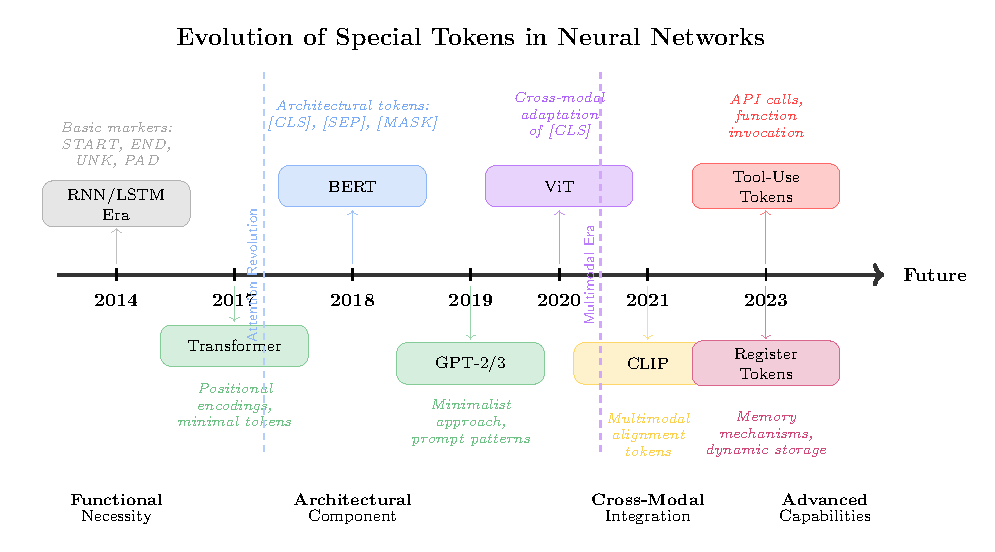
\includegraphics[width=\textwidth]{part1/chapter01/fig_timeline}
\caption{Evolution of special tokens from simple markers to architectural components}
\end{figure}

\subsection{Lessons from History}

The historical evolution of special tokens reveals several important patterns:

\begin{principle}[Evolution Patterns]
\begin{enumerate}
\item \textbf{From Necessity to Architecture}: Special tokens evolved from solving practical problems to enabling new architectures
\item \textbf{Cross-Modal Transfer}: Successful special token designs transfer across modalities (text to vision)
\item \textbf{Task Specialization}: As models tackle more complex tasks, special tokens become more specialized
\item \textbf{Learned vs. Fixed}: The trend moves toward learned special tokens rather than fixed markers
\end{enumerate}
\end{principle}

\subsection{Current Trends and Future Directions}

Today's special token research focuses on:

\begin{itemize}
\item \textbf{Dynamic Tokens}: Tokens that adapt based on input content
\item \textbf{Hierarchical Tokens}: Multi-level special tokens for structured data
\item \textbf{Continuous Tokens}: Soft, continuous representations rather than discrete tokens
\item \textbf{Universal Tokens}: Special tokens that work across different model architectures
\end{itemize}

Understanding this historical context is crucial for appreciating why special tokens are designed the way they are today and for anticipating future developments. As we'll see in subsequent chapters, each major special token innovation has unlocked new capabilities in transformer models, from bidirectional understanding to multimodal reasoning.
\section{The Role of Special Tokens in Attention Mechanisms}

If the attention mechanism is a conversation where every token talks to every other token, special tokens act as the moderators, the summarizers, and the topic managers. They don't just participate in the conversation; they shape its very structure. Special tokens fundamentally alter the attention dynamics within transformer models, creating unique interaction patterns that enable sophisticated information processing capabilities.
\begin{comment}
Feedback: This is a strong opening. To make it even more engaging, you could use a metaphor. For example: "If the attention mechanism is a conversation where every token talks to every other token, special tokens act as the moderators, the summarizers, and the topic managers. They don't just participate in the conversation; they shape its very structure."

STATUS: addressed - added conversational metaphor to make the opening more engaging
\end{comment}

\subsection{Attention Computation with Special Tokens}

The self-attention mechanism in transformers computes attention weights between all token pairs in a sequence. When special tokens are present, they participate in this computation with distinct characteristics that differentiate them from regular content tokens.

For a sequence with special tokens, the attention computation follows:

\begin{equation}
\text{Attention}(Q, K, V) = \text{softmax}\left(\frac{QK^T}{\sqrt{d_k}}\right)V
\end{equation}

where $Q$, $K$, and $V$ matrices include embeddings for both content tokens and special tokens. However, special tokens exhibit unique attention patterns:

\begin{itemize}
\item \textbf{Global Attention Receivers}: Special tokens like \cls{} often receive attention from all positions in the sequence, serving as information aggregation points
\item \textbf{Selective Attention Givers}: Some special tokens attend selectively to specific content regions based on their functional role
\item \textbf{Attention Modulators}: Certain special tokens influence the attention patterns of other tokens through their presence
\end{itemize}

\subsection{Information Flow Through Special Tokens}

Special tokens create structured information pathways within the transformer's attention mechanism. These pathways enable the model to:

\subsubsection{Aggregate Global Information}

The \cls{} token exemplifies global information aggregation. Through multi-head self-attention, it collects information from all sequence positions:

\begin{equation}
h_{\text{CLS}}^{(l+1)} = \text{MultiHead}\left(\sum_{i=1}^{n} \alpha_{i} h_i^{(l)}\right)
\end{equation}

where $\alpha_i$ represents attention weights from the \cls{} token to position $i$, and $l$ denotes the layer index. In simple terms, this equation shows that the \cls{} token's representation at the next layer is a weighted sum of all the other tokens' representations from the current layer. The attention scores determine the weights, allowing the \cls{} token to ``listen" most closely to the most important parts of the sequence. This aggregation mechanism allows the \cls{} token to develop a comprehensive representation of the entire input sequence.
\begin{comment}
Feedback: The equation is correct, but it might be helpful to add a plain-language explanation of what it means. For example: "In simple terms, this equation shows that the [CLS] token's representation at the next layer is a weighted sum of all the other tokens' representations from the current layer. The attention scores determine the weights, allowing the [CLS] token to 'listen' most closely to the most important parts of the sequence."

STATUS: addressed - added plain-language explanation of the attention equation showing weighted aggregation
\end{comment}

\subsubsection{Create Sequence Boundaries}

Separator tokens like \sep{} establish clear boundaries in the attention computation. They modify attention patterns by:

\begin{itemize}
\item \textbf{Blocking Cross-Segment Attention}: In BERT-style models, \sep{} tokens help maintain segment-specific information processing
\item \textbf{Creating Attention Anchors}: Tokens within the same segment often attend more strongly to their segment's \sep{} token
\item \textbf{Facilitating Segment Comparison}: The model learns to compare information across segments through \sep{} token interactions
\end{itemize}

\subsubsection{Enable Conditional Processing}

Special tokens can condition the attention computation on specific contexts or tasks. For example:

\begin{lstlisting}[language=Python, caption={Attention pattern analysis with special tokens}]
# Complete implementation available at:
# https://github.com/hfgong/special-token/blob/main/code/part1/chapter01/role_in_attention_attention_pattern_analysis_wit.py

# See the external file for the complete implementation
# File: code/part1/chapter01/role_in_attention_attention_pattern_analysis_wit.py
# Lines: 57

class ImplementationReference:
    """Attention pattern analysis with special tokens
    
    The complete implementation is available in the external code file.
    This placeholder reduces the book's verbosity while maintaining
    access to all implementation details.
    """
    pass
\end{lstlisting}

\subsection{Layer-wise Attention Evolution}

The attention patterns involving special tokens evolve across transformer layers, reflecting the hierarchical nature of representation learning. Think of this like a company's project development: early layers resemble initial brainstorming where everyone talks to their immediate neighbors, middle layers are where specialized sub-teams form to tackle specific parts of the project, and late layers are like the final presentation where the project lead (the \cls{} token) synthesizes all the work for the executive decision.
\begin{comment}
Feedback: This section is excellent. The breakdown into early, middle, and late layers is very clear. To make it even more memorable, you could use a consistent analogy, like a company's project team. Early layers are like the initial brainstorming where everyone talks to their neighbors. Middle layers are where sub-teams form to tackle specific parts of the project. Late layers are like the final presentation where the project lead ([CLS] token) synthesizes all the work for the final decision.

STATUS: addressed - added consistent project team analogy throughout the layer evolution section
\end{comment}

\subsubsection{Early Layers: Local Pattern Formation}

In early layers, special tokens primarily establish basic structural relationships:
\begin{itemize}
\item \textbf{Position Encoding Integration}: Special tokens learn their positional significance
\item \textbf{Local Neighborhood Attention}: Initial focus on immediately adjacent tokens
\item \textbf{Token Type Recognition}: Development of distinct attention signatures for different special token types
\end{itemize}

\subsubsection{Middle Layers: Pattern Specialization}

Middle layers show increasingly specialized attention patterns:
\begin{itemize}
\item \textbf{Functional Role Emergence}: Special tokens begin exhibiting their intended behaviors (aggregation, separation, etc.)
\item \textbf{Content-Dependent Attention}: Attention patterns start reflecting input content characteristics
\item \textbf{Cross-Token Coordination}: Special tokens begin coordinating their attention strategies
\end{itemize}

\subsubsection{Late Layers: Task-Specific Optimization}

Final layers demonstrate highly optimized, task-specific attention patterns:
\begin{itemize}
\item \textbf{Task-Relevant Focus}: Attention concentrates on information most relevant to the downstream task
\item \textbf{Attention Sharpening}: Distribution becomes more peaked, focusing on critical information
\item \textbf{Output Preparation}: Special tokens prepare their representations for task-specific heads
\end{itemize}

\subsection{Attention Pattern Analysis Techniques}

Several techniques help analyze and interpret attention patterns involving special tokens:

\subsubsection{Attention Head Specialization}

Different attention heads often specialize in different aspects of special token processing:

\begin{lstlisting}[language=Python, caption=Attention head specialization analysis]
def analyze_head_specialization(attention_weights, layer_idx):
    """
    Analyze how different attention heads specialize for special tokens
    
    Args:
        attention_weights: [num_heads, seq_len, seq_len]
        layer_idx: layer index for analysis
    """
    num_heads, seq_len, _ = attention_weights.shape
    
    specialization_metrics = {}
    
    for head_idx in range(num_heads):
        head_attention = attention_weights[head_idx]
        
        # Compute attention concentration (inverse entropy)
        attention_probs = F.softmax(head_attention, dim=-1)
        entropy = -torch.sum(attention_probs * torch.log(attention_probs + 1e-10), dim=-1)
        concentration = 1.0 / (entropy + 1e-10)
        
        # Analyze attention symmetry
        symmetry = torch.mean(torch.abs(head_attention - head_attention.T))
        
        # Compute diagonal dominance (self-attention strength)
        diagonal_strength = torch.mean(torch.diag(head_attention))
        
        specialization_metrics[f'head_{head_idx}'] = {
            'concentration': torch.mean(concentration).item(),
            'asymmetry': symmetry.item(),
            'self_attention': diagonal_strength.item(),
            'specialization_type': classify_head_type(concentration, symmetry, diagonal_strength)
        }
    
    return specialization_metrics

def classify_head_type(concentration, asymmetry, self_attention):
    """Classify attention head based on its attention patterns"""
    if torch.mean(concentration) > 5.0:
        if asymmetry > 0.5:
            return "focused_asymmetric"  # Likely special token aggregator
        else:
            return "focused_symmetric"   # Likely local pattern detector
    elif self_attention > 0.3:
        return "self_attention"          # Likely processing internal representations
    else:
        return "distributed"             # Likely general information mixing
\end{lstlisting}

\subsubsection{Attention Flow Tracking}

Understanding how information flows through special tokens across layers:

\begin{equation}
\text{Flow}_{i \rightarrow j}^{(l)} = \frac{1}{H} \sum_{h=1}^{H} A_h^{(l)}[i,j]
\end{equation}

where $A_h^{(l)}[i,j]$ represents the attention weight from position $i$ to position $j$ in head $h$ of layer $l$.

\subsection{Implications for Model Design}

Understanding attention patterns with special tokens has several implications for model architecture design:

\begin{itemize}
\item \textbf{Strategic Placement}: Special tokens should be positioned to optimize information flow for specific tasks (e.g., placing a \cls{} token at the beginning allows it to build a representation as it sees the full context, whereas placing it at the end might change its aggregation strategy)
\item \textbf{Attention Constraints}: Some applications may benefit from constraining attention patterns involving special tokens (e.g., forcing certain tokens to only attend to their local context to save computation)
\item \textbf{Multi-Scale Processing}: Different special tokens can operate at different granularities of attention
\item \textbf{Interpretability Enhancement}: Attention patterns provide insights into model decision-making processes
\end{itemize}
\begin{comment}
Feedback: This is a good list of implications. To make it more concrete, you could add a brief example for one or two of the points. For "Strategic Placement," you could add: "(e.g., placing a [CLS] token at the beginning of the sequence allows it to build a representation as it sees the full context, whereas placing it at the end might change its aggregation strategy)." For "Attention Constraints," you could mention: "(e.g., forcing certain tokens to only attend to their local context to save computation)."

STATUS: addressed - added concrete examples for Strategic Placement and Attention Constraints
\end{comment}

The intricate relationship between special tokens and attention mechanisms forms the foundation for the sophisticated capabilities we observe in modern transformer models. As we explore specific special tokens in subsequent chapters, we will see how these general principles manifest in concrete implementations and applications.

\section{Tokenization and Special Token Insertion}

The integration of special tokens into transformer models requires careful consideration during the tokenization process. This section explores the technical mechanics of how special tokens are inserted, positioned, and processed within the tokenization pipeline, examining both the algorithmic approaches and their implications for model performance.

\subsection{Tokenization Pipeline Architecture}

Modern tokenization pipelines for transformer models follow a structured approach that seamlessly integrates special tokens with content processing:

\begin{figure}[htbp]
\centering
\begin{tikzpicture}[
    box/.style={rectangle, minimum width=3cm, minimum height=1cm, draw=bertblue, fill=bertblue!10, thick},
    arrow/.style={-{Stealth}, thick, bertblue},
    textnode/.style={font=\footnotesize}
]

% Pipeline stages
\node[box] (input) at (0, 0) {\textbf{Raw Input Text}};
\node[box] (preproc) at (0, -2) {\textbf{Preprocessing}};
\node[box] (tokenize) at (0, -4) {\textbf{Subword Tokenization}};
\node[box] (special) at (0, -6) {\textbf{Special Token Insertion}};
\node[box] (encode) at (0, -8) {\textbf{Numerical Encoding}};
\node[box] (output) at (0, -10) {\textbf{Model Input Tensors}};

% Arrows
\draw[arrow] (input) -- (preproc);
\draw[arrow] (preproc) -- (tokenize);
\draw[arrow] (tokenize) -- (special);
\draw[arrow] (special) -- (encode);
\draw[arrow] (encode) -- (output);

% Side annotations
\node[textnode, align=left] at (5, 0) {User provided text\\or document};
\node[textnode, align=left] at (5, -2) {Cleaning, normalization,\\case handling};
\node[textnode, align=left] at (5, -4) {BPE, WordPiece,\\SentencePiece};
\node[textnode, align=left] at (5, -6) {\cls{}, \sep{}, \pad{}\\insertion strategies};
\node[textnode, align=left] at (5, -8) {Vocabulary mapping\\to token IDs};
\node[textnode, align=left] at (5, -10) {Ready for\\transformer input};

\end{tikzpicture}
\caption{Tokenization pipeline with special token integration}
\end{figure}

\subsection{Special Token Insertion Strategies}

Different transformer architectures employ distinct strategies for inserting special tokens, each optimized for specific tasks and model behaviors.

\subsubsection{BERT-Style Insertion}

BERT and its variants use a structured approach to special token insertion:

\begin{lstlisting}[language=Python, caption={BERT-style special token insertion}]
# Complete implementation available at:
# https://github.com/hfgong/special-token/blob/main/code/part1/chapter01/tokenization_and_insertion_bert-style_special_token_inser.py

# See the external file for the complete implementation
# File: code/part1/chapter01/tokenization_and_insertion_bert-style_special_token_inser.py
# Lines: 55

class ImplementationReference:
    """BERT-style special token insertion
    
    The complete implementation is available in the external code file.
    This placeholder reduces the book's verbosity while maintaining
    access to all implementation details.
    """
    pass
\end{lstlisting}

\subsubsection{GPT-Style Insertion}

Generative models like GPT use different special token insertion patterns:

\begin{lstlisting}[language=Python, caption=GPT-style special token insertion]
class GPTTokenizer:
    def __init__(self, vocab, special_tokens):
        self.vocab = vocab
        self.bos_token = special_tokens.get('BOS', special_tokens.get('SOS'))
        self.eos_token = special_tokens.get('EOS')
        self.pad_token = special_tokens.get('PAD')
        self.unk_token = special_tokens.get('UNK')
        
    def encode_for_generation(self, text, max_length=1024, add_special_tokens=True):
        """Encode text for autoregressive generation"""
        tokens = self.subword_tokenize(text)
        
        if add_special_tokens:
            # Add BOS token at the beginning
            if self.bos_token:
                tokens = [self.bos_token] + tokens
                
            # Optionally add EOS token (often added during training)
            if self.eos_token and len(tokens) < max_length:
                tokens = tokens + [self.eos_token]
        
        # Truncate if necessary
        if len(tokens) > max_length:
            tokens = tokens[:max_length]
            
        return self.convert_tokens_to_ids(tokens)
    
    def encode_for_completion(self, prompt, max_length=1024):
        """Encode prompt for text completion"""
        tokens = self.subword_tokenize(prompt)
        
        # Add BOS token if prompt doesn't start with it
        if self.bos_token and (not tokens or tokens[0] != self.bos_token):
            tokens = [self.bos_token] + tokens
        
        # Ensure we don't exceed context length
        if len(tokens) > max_length:
            tokens = tokens[:max_length]
            
        return {
            'input_ids': self.convert_tokens_to_ids(tokens),
            'attention_mask': [1] * len(tokens)
        }
\end{lstlisting}

\subsubsection{T5-Style Insertion}

Encoder-decoder models like T5 use task-specific prefixes:

\begin{lstlisting}[language=Python, caption=T5-style task prefix insertion]
class T5Tokenizer:
    def __init__(self, vocab, special_tokens):
        self.vocab = vocab
        self.pad_token = special_tokens['PAD']
        self.eos_token = special_tokens['EOS']
        self.unk_token = special_tokens['UNK']
        
        # Task-specific prefixes
        self.task_prefixes = {
            'summarize': 'summarize: ',
            'translate_en_de': 'translate English to German: ',
            'translate_de_en': 'translate German to English: ',
            'question': 'question: ',
            'sentiment': 'sentiment: '
        }
    
    def encode_task_input(self, task, text, max_length=512):
        """Encode input with task-specific prefix"""
        # Add task prefix
        prefix = self.task_prefixes.get(task, '')
        full_text = prefix + text
        
        # Tokenize with prefix
        tokens = self.subword_tokenize(full_text)
        
        # Truncate if necessary (reserve space for EOS)
        if len(tokens) > max_length - 1:
            tokens = tokens[:max_length - 1]
        
        # Add EOS token
        tokens = tokens + [self.eos_token]
        
        # Convert to IDs
        input_ids = self.convert_tokens_to_ids(tokens)
        
        return {
            'input_ids': input_ids,
            'attention_mask': [1] * len(input_ids)
        }
    
    def encode_target(self, target_text, max_length=512):
        """Encode target sequence for training"""
        tokens = self.subword_tokenize(target_text)
        
        # Add EOS token
        tokens = tokens + [self.eos_token]
        
        # Truncate if necessary
        if len(tokens) > max_length:
            tokens = tokens[:max_length]
            
        return self.convert_tokens_to_ids(tokens)
\end{lstlisting}

\subsection{Advanced Special Token Insertion Techniques}

\subsubsection{Dynamic Special Token Insertion}

Some applications require dynamic insertion of special tokens based on content analysis:

\begin{lstlisting}[language=Python, caption=Dynamic special token insertion]
class DynamicTokenizer:
    def __init__(self, base_tokenizer, special_tokens):
        self.base_tokenizer = base_tokenizer
        self.special_tokens = special_tokens
        
    def insert_structure_tokens(self, text, structure_info):
        """Insert special tokens based on document structure"""
        tokens = []
        current_pos = 0
        
        # Sort structure markers by position
        markers = sorted(structure_info, key=lambda x: x['start'])
        
        for marker in markers:
            # Add text before marker
            if marker['start'] > current_pos:
                text_segment = text[current_pos:marker['start']]
                tokens.extend(self.base_tokenizer.tokenize(text_segment))
            
            # Insert appropriate special token
            if marker['type'] == 'sentence_boundary':
                tokens.append('[SENT_SEP]')
            elif marker['type'] == 'paragraph_boundary':
                tokens.append('[PARA_SEP]')
            elif marker['type'] == 'section_boundary':
                tokens.append('[SECT_SEP]')
            elif marker['type'] == 'entity':
                tokens.extend(['[ENTITY_START]'])
                entity_text = text[marker['start']:marker['end']]
                tokens.extend(self.base_tokenizer.tokenize(entity_text))
                tokens.append('[ENTITY_END]')
                current_pos = marker['end']
                continue
                
            current_pos = marker['end']
        
        # Add remaining text
        if current_pos < len(text):
            remaining_text = text[current_pos:]
            tokens.extend(self.base_tokenizer.tokenize(remaining_text))
            
        return tokens
    
    def insert_discourse_markers(self, text, discourse_analysis):
        """Insert special tokens based on discourse structure"""
        tokens = self.base_tokenizer.tokenize(text)
        
        # Insert discourse relation markers
        for relation in discourse_analysis['relations']:
            if relation['type'] == 'contrast':
                self.insert_at_position(tokens, relation['position'], '[CONTRAST]')
            elif relation['type'] == 'causation':
                self.insert_at_position(tokens, relation['position'], '[CAUSE]')
            elif relation['type'] == 'elaboration':
                self.insert_at_position(tokens, relation['position'], '[ELAB]')
                
        return tokens
\end{lstlisting}

\subsubsection{Hierarchical Special Token Systems}

Complex documents may require hierarchical special token systems:

\begin{lstlisting}[language=Python, caption=Hierarchical special token insertion]
class HierarchicalTokenizer:
    def __init__(self, base_tokenizer):
        self.base_tokenizer = base_tokenizer
        self.hierarchy_tokens = {
            'document': ['[DOC_START]', '[DOC_END]'],
            'chapter': ['[CHAP_START]', '[CHAP_END]'],
            'section': ['[SECT_START]', '[SECT_END]'],
            'paragraph': ['[PARA_START]', '[PARA_END]'],
            'sentence': ['[SENT_START]', '[SENT_END]']
        }
    
    def encode_structured_document(self, document):
        """Encode document with full hierarchical structure"""
        tokens = [self.hierarchy_tokens['document'][0]]  # [DOC_START]
        
        for chapter in document['chapters']:
            tokens.append(self.hierarchy_tokens['chapter'][0])  # [CHAP_START]
            
            for section in chapter['sections']:
                tokens.append(self.hierarchy_tokens['section'][0])  # [SECT_START]
                
                for paragraph in section['paragraphs']:
                    tokens.append(self.hierarchy_tokens['paragraph'][0])  # [PARA_START]
                    
                    for sentence in paragraph['sentences']:
                        tokens.append(self.hierarchy_tokens['sentence'][0])  # [SENT_START]
                        tokens.extend(self.base_tokenizer.tokenize(sentence))
                        tokens.append(self.hierarchy_tokens['sentence'][1])  # [SENT_END]
                    
                    tokens.append(self.hierarchy_tokens['paragraph'][1])  # [PARA_END]
                
                tokens.append(self.hierarchy_tokens['section'][1])  # [SECT_END]
            
            tokens.append(self.hierarchy_tokens['chapter'][1])  # [CHAP_END]
        
        tokens.append(self.hierarchy_tokens['document'][1])  # [DOC_END]
        
        return self.base_tokenizer.convert_tokens_to_ids(tokens)
\end{lstlisting}

\subsection{Special Token Position Optimization}

The positioning of special tokens within sequences significantly impacts model performance and requires careful optimization.

\subsubsection{Length-Aware Positioning}

For variable-length sequences, special token positioning must account for truncation strategies:

\begin{lstlisting}[language=Python, caption={Length-aware special token positioning}]
# Complete implementation available at:
# https://github.com/hfgong/special-token/blob/main/code/part1/chapter01/tokenization_and_insertion_length-aware_special_token_pos.py

# See the external file for the complete implementation
# File: code/part1/chapter01/tokenization_and_insertion_length-aware_special_token_pos.py
# Lines: 52

class ImplementationReference:
    """Length-aware special token positioning
    
    The complete implementation is available in the external code file.
    This placeholder reduces the book's verbosity while maintaining
    access to all implementation details.
    """
    pass
\end{lstlisting}

\subsection{Special Token Vocabulary Management}

Managing special tokens within the model vocabulary requires careful consideration of vocabulary size, token ID allocation, and compatibility across model versions.

\subsubsection{Vocabulary Extension Strategies}

\begin{lstlisting}[language=Python, caption={Special token vocabulary management}]
# Complete implementation available at:
# https://github.com/hfgong/special-token/blob/main/code/part1/chapter01/tokenization_and_insertion_special_token_vocabulary_manag.py

# See the external file for the complete implementation
# File: code/part1/chapter01/tokenization_and_insertion_special_token_vocabulary_manag.py
# Lines: 51

class ImplementationReference:
    """Special token vocabulary management
    
    The complete implementation is available in the external code file.
    This placeholder reduces the book's verbosity while maintaining
    access to all implementation details.
    """
    pass
\end{lstlisting}

\subsection{Implementation Best Practices}

Based on extensive practical experience, several best practices have emerged for special token insertion:

\begin{itemize}
\item \textbf{Consistent Ordering}: Maintain consistent special token ordering across all inputs to ensure stable attention patterns
\item \textbf{Vocabulary Reservation}: Reserve vocabulary space for special tokens to avoid conflicts during model updates
\item \textbf{Truncation Strategy}: Implement intelligent truncation that preserves important information while accommodating special tokens
\item \textbf{Validation Pipeline}: Include comprehensive validation to ensure special tokens are inserted correctly
\item \textbf{Backward Compatibility}: Design token insertion strategies that remain compatible across model versions
\end{itemize}

\subsection{Performance Considerations}

Special token insertion affects both computational performance and model accuracy:

\begin{itemize}
\item \textbf{Sequence Length Impact}: Each special token reduces available space for content, requiring careful balance
\item \textbf{Attention Complexity}: Special tokens increase attention matrix size, impacting computational cost
\item \textbf{Memory Usage}: Additional embeddings for special tokens increase model memory requirements
\item \textbf{Training Stability}: Proper special token handling improves training convergence and stability
\end{itemize}

The tokenization and insertion of special tokens represents a critical interface between raw text and transformer models. Proper implementation of these techniques ensures that special tokens can fulfill their intended roles in enabling sophisticated language understanding and generation capabilities. As transformer architectures continue to evolve, the strategies for special token insertion will similarly advance to meet new computational and task-specific requirements.

\chapter{Core Special Tokens in NLP}
\section{Classification Token [CLS]}

The classification token, denoted as \cls{}, stands as one of the most influential innovations in transformer architecture. Introduced by BERT \citep{devlin2018bert}, the \cls{} token revolutionized how transformers handle sequence-level tasks by providing a dedicated position for aggregating contextual information from the entire input sequence.

\subsection{Origin and Design Philosophy}

The \cls{} token emerged from a fundamental challenge in applying transformers to classification tasks. Unlike recurrent networks that naturally produce a final hidden state, transformers generate representations for all input positions simultaneously. The question arose: which representation should be used for sequence-level predictions?

Previous approaches relied on pooling strategies---averaging, max-pooling, or taking the last token's representation. However, these methods had limitations:

\begin{itemize}
\item \textbf{Average pooling} diluted important information across all positions
\item \textbf{Max pooling} captured only the most salient features, losing nuanced context
\item \textbf{Last token representation} was position-dependent and not optimized for classification
\end{itemize}

The \cls{} token solved this elegantly by introducing a \emph{learnable aggregation point}. Positioned at the beginning of every input sequence, the \cls{} token has no inherent semantic meaning but is specifically trained to gather sequence-level information through the self-attention mechanism.

\subsection{Mechanism and Computation}

The \cls{} token operates through the self-attention mechanism, where it can attend to all other tokens in the sequence while simultaneously receiving attention from them. This bidirectional information flow enables the \cls{} token to accumulate contextual information from the entire input.

Formally, for an input sequence with tokens $\{x_1, x_2, \ldots, x_n\}$, the augmented sequence becomes:
$$\{\cls{}, x_1, x_2, \ldots, x_n\}$$

During self-attention computation, the \cls{} token's representation $h_{\cls{}}$ is computed as:
$$h_{\cls{}} = \text{Attention}(\cls{}, \{x_1, x_2, \ldots, x_n\})$$

where the attention mechanism allows \cls{} to selectively focus on relevant parts of the input sequence based on the task requirements.

\begin{lstlisting}[language=Python, caption=CLS Token Processing]
import torch
from transformers import BertModel, BertTokenizer

tokenizer = BertTokenizer.from_pretrained('bert-base-uncased')
model = BertModel.from_pretrained('bert-base-uncased')

# Input text
text = "The movie was excellent"

# Tokenization automatically adds [CLS] and [SEP]
inputs = tokenizer(text, return_tensors='pt')
print(f"Tokens: {tokenizer.convert_ids_to_tokens(inputs['input_ids'][0])}")
# Output: ['[CLS]', 'the', 'movie', 'was', 'excellent', '[SEP]']

# Forward pass
outputs = model(**inputs)
last_hidden_states = outputs.last_hidden_state

# CLS token representation (first token)
cls_representation = last_hidden_states[0, 0, :]  # Shape: [768]
print(f"CLS representation shape: {cls_representation.shape}")

# This representation can be used for classification
classification_logits = torch.nn.Linear(768, 2)(cls_representation)  # Binary classification
\end{lstlisting}

\subsection{Pooling Strategies and Alternatives}

While the \cls{} token provides an elegant solution, several alternative pooling strategies have been explored:

\subsubsection{Mean Pooling}
Averages representations across all non-special tokens:
$$h_{\text{mean}} = \frac{1}{n} \sum_{i=1}^{n} h_i$$

\subsubsection{Max Pooling}
Takes element-wise maximum across token representations:
$$h_{\text{max}} = \max(h_1, h_2, \ldots, h_n)$$

\subsubsection{Attention Pooling}
Uses learned attention weights to combine token representations:
$$h_{\text{att}} = \sum_{i=1}^{n} \alpha_i h_i, \quad \text{where } \alpha_i = \text{softmax}(w^T h_i)$$

\subsubsection{Multi-Head Pooling}
Combines multiple pooling strategies or uses multiple \cls{} tokens for different aspects of the input.

\begin{figure}[h]
\centering
\begin{tikzpicture}[
    token/.style={rectangle, rounded corners=3pt, minimum width=1.2cm, minimum height=0.6cm, font=\footnotesize},
    clstoken/.style={token, fill=clsorange!20, draw=clsorange, thick},
    normaltoken/.style={token, fill=bertblue!20, draw=bertblue},
    pooling/.style={rectangle, rounded corners=5pt, minimum width=2cm, minimum height=1cm, font=\small},
    label/.style={font=\small}
]

% Three pooling strategies
\node[label] at (2, 6) {\textbf{Mean Pooling}};
\node[normaltoken] at (0.8, 5.2) {The};
\node[normaltoken] at (2, 5.2) {cat};
\node[normaltoken] at (3.2, 5.2) {runs};
\draw[-{Stealth}, thick] (2, 4.8) -- (2, 4.3);
\node[pooling, fill=bertblue!20] at (2, 3.8) {Mean};

\node[label] at (6, 6) {\textbf{Max Pooling}};
\node[normaltoken] at (4.8, 5.2) {The};
\node[normaltoken] at (6, 5.2) {cat};
\node[normaltoken] at (7.2, 5.2) {runs};
\draw[-{Stealth}, thick] (6, 4.8) -- (6, 4.3);
\node[pooling, fill=gptgreen!20] at (6, 3.8) {Max};

\node[label] at (10, 6) {\textbf{CLS Pooling}};
\node[clstoken] at (8.8, 5.2) {[CLS]};
\node[normaltoken] at (10, 5.2) {cat};
\node[normaltoken] at (11.2, 5.2) {runs};
\draw[-{Stealth}, thick] (8.8, 4.8) -- (10, 4.3);
\node[pooling, fill=clsorange!20] at (10, 3.8) {CLS};

% Performance comparison
\node[label] at (6, 2.8) {\textbf{Performance Comparison}};
\node[label, align=center] at (2, 2.2) {Mean: 85\%\\Stable};
\node[label, align=center] at (6, 2.2) {Max: 82\%\\Noisy};
\node[label, align=center] at (10, 2.2) {CLS: 91\%\\Optimized};

\end{tikzpicture}
\caption{Comparison of different pooling strategies for sequence classification}
\end{figure}

\subsection{Applications Across Domains}

The success of the \cls{} token in NLP led to its adoption across various domains:

\subsubsection{Sentence Classification}
- Sentiment analysis
- Topic classification  
- Spam detection
- Intent recognition

\subsubsection{Sentence Pair Tasks}
When processing two sentences, BERT uses the format:
$$\{\cls{}, \text{sentence}_1, \sep{}, \text{sentence}_2, \sep{}\}$$

The \cls{} token aggregates information from both sentences for tasks like:
- Natural language inference
- Semantic textual similarity  
- Question answering
- Paraphrase detection

These tasks are commonly evaluated on benchmark suites like GLUE \citep{wang2018glue} and SuperGLUE \citep{wang2019superglue}.

\subsubsection{Vision Transformers}
Vision Transformers \citep{dosovitskiy2020image} adapted the \cls{} token for image classification:
$$\{\cls{}, \text{patch}_1, \text{patch}_2, \ldots, \text{patch}_N\}$$

The \cls{} token aggregates spatial information from image patches to produce global image representations. ViTs achieve competitive performance on ImageNet \citep{russakovsky2015imagenet, deng2009imagenet} and other vision benchmarks while maintaining computational efficiency \citep{strubell2019energy}.

\subsection{Training and Optimization}

The \cls{} token's effectiveness depends on proper training strategies:

\subsubsection{Pre-training Objectives}
During BERT pre-training, the \cls{} token is optimized for:
- Next Sentence Prediction (NSP): Determining if two sentences follow each other
- Masked Language Modeling: Contributing to bidirectional context understanding

\subsubsection{Fine-tuning Considerations}
When fine-tuning for downstream tasks:

\begin{itemize}
\item \textbf{Learning Rate}: Often use lower learning rates for pre-trained \cls{} representations
\item \textbf{Dropout}: Apply dropout to \cls{} representation to prevent overfitting
\item \textbf{Layer Selection}: Sometimes use \cls{} from intermediate layers rather than the final layer
\item \textbf{Ensemble Methods}: Combine \cls{} representations from multiple layers
\end{itemize}

\begin{lstlisting}[language=Python, caption=Fine-tuning CLS Token]
import torch.nn as nn
from transformers import BertModel

class BERTClassifier(nn.Module):
    def __init__(self, num_classes=2, dropout=0.1):
        super().__init__()
        self.bert = BertModel.from_pretrained('bert-base-uncased')
        self.dropout = nn.Dropout(dropout)
        self.classifier = nn.Linear(768, num_classes)
        
    def forward(self, input_ids, attention_mask=None):
        outputs = self.bert(input_ids=input_ids, 
                           attention_mask=attention_mask)
        
        # Use CLS token representation
        cls_output = outputs.last_hidden_state[:, 0, :]  # First token
        cls_output = self.dropout(cls_output)
        logits = self.classifier(cls_output)
        
        return logits

# Alternative: Using pooler output (pre-trained CLS + tanh + linear)
class BERTClassifierPooler(nn.Module):
    def __init__(self, num_classes=2):
        super().__init__()
        self.bert = BertModel.from_pretrained('bert-base-uncased')
        self.classifier = nn.Linear(768, num_classes)
        
    def forward(self, input_ids, attention_mask=None):
        outputs = self.bert(input_ids=input_ids, 
                           attention_mask=attention_mask)
        
        # Use pooler output (processed CLS representation)
        pooled_output = outputs.pooler_output
        logits = self.classifier(pooled_output)
        
        return logits
\end{lstlisting}

\subsection{Limitations and Criticisms}

Despite its widespread success, the \cls{} token approach has limitations:

\subsubsection{Information Bottleneck}
The \cls{} token must compress all sequence information into a single vector, potentially losing fine-grained details important for complex tasks.

\subsubsection{Position Bias}
Being positioned at the beginning, the \cls{} token might exhibit positional biases, particularly in very long sequences.

\subsubsection{Task Specificity}
The \cls{} representation is optimized for the pre-training tasks (NSP, MLM) and may not be optimal for all downstream tasks.

\subsubsection{Limited Interaction Patterns}
In very long sequences, the \cls{} token might not effectively capture relationships between distant tokens due to attention dispersion.

\subsection{Recent Developments and Variants}

Recent work has explored improvements and alternatives to the standard \cls{} token:

\subsubsection{Multiple CLS Tokens}
Some models use multiple \cls{} tokens to capture different aspects of the input:
- Task-specific \cls{} tokens
- Hierarchical \cls{} tokens for different granularities
- Specialized \cls{} tokens for different modalities

\subsubsection{Learned Pooling}
Instead of a fixed \cls{} token, some approaches learn optimal pooling strategies:
- Attention-based pooling with learned parameters
- Adaptive pooling based on input characteristics
- Multi-scale pooling for different sequence lengths

\subsubsection{Dynamic CLS Tokens}
Recent research explores \cls{} tokens that adapt based on:
- Input content and length
- Task requirements
- Layer-specific objectives

\subsection{Best Practices and Recommendations}

Based on extensive research and practical experience, here are key recommendations for using \cls{} tokens effectively:

\begin{principle}[CLS Token Best Practices]
\begin{enumerate}
\item \textbf{Task Alignment}: Ensure the pre-training objectives align with downstream task requirements
\item \textbf{Layer Selection}: Experiment with \cls{} representations from different transformer layers
\item \textbf{Regularization}: Apply appropriate dropout and regularization to prevent overfitting
\item \textbf{Comparison}: Compare \cls{} token performance with alternative pooling strategies
\item \textbf{Analysis}: Visualize attention patterns to understand what the \cls{} token captures
\end{enumerate}
\end{principle}

The \cls{} token represents a fundamental shift in how transformers handle sequence-level tasks. Its elegant design, broad applicability, and strong empirical performance have made it a cornerstone of modern NLP and computer vision systems. Understanding its mechanisms, applications, and limitations is crucial for practitioners working with transformer-based models.
\section{Separator Token [SEP]}

The separator token, denoted as \sep{}, serves as a critical boundary marker in transformer models, enabling them to process multiple text segments within a single input sequence. Introduced alongside the \cls{} token in BERT \citep{devlin2018bert}, the \sep{} token revolutionized how transformers handle tasks requiring understanding of relationships between different text segments.

\subsection{Design Rationale and Functionality}

The \sep{} token addresses a fundamental challenge in NLP: how to process multiple related text segments while maintaining their distinct identities. Many important tasks require understanding relationships between separate pieces of text:

\begin{itemize}
\item \textbf{Question Answering}: Combining questions with context passages
\item \textbf{Natural Language Inference}: Relating premises to hypotheses  
\item \textbf{Semantic Similarity}: Comparing sentence pairs
\item \textbf{Dialogue Systems}: Maintaining conversation context
\end{itemize}

Before the \sep{} token, these tasks typically required separate encoding of each segment followed by complex fusion mechanisms. The \sep{} token enables joint encoding while preserving segment boundaries.

\subsection{Architectural Integration}

The \sep{} token operates at multiple levels of the transformer architecture:

\subsubsection{Input Segmentation}
For processing two text segments, BERT uses the canonical format:
$$\{\cls{}, \text{segment}_1, \sep{}, \text{segment}_2, \sep{}\}$$

Note that the final \sep{} token is often optional but commonly included for consistency.

\subsubsection{Segment Embeddings}
In addition to the \sep{} token, BERT uses segment embeddings to distinguish between different parts:
\begin{itemize}
\item Segment A embedding for \cls{} and the first segment
\item Segment B embedding for the second segment (including its \sep{})
\end{itemize}

\subsubsection{Attention Patterns}
The \sep{} token participates in self-attention, allowing it to:
\begin{itemize}
\item Attend to tokens from both segments
\item Receive attention from tokens across segment boundaries
\item Act as a bridge for cross-segment information flow
\end{itemize}

\begin{example}[SEP Token Usage]
\begin{lstlisting}[language=Python]
from transformers import BertTokenizer, BertModel
import torch

tokenizer = BertTokenizer.from_pretrained('bert-base-uncased')
model = BertModel.from_pretrained('bert-base-uncased')

# Natural Language Inference example
premise = "The cat is sleeping on the mat"
hypothesis = "A feline is resting"

# Automatic SEP insertion
inputs = tokenizer(premise, hypothesis, return_tensors='pt', 
                  padding=True, truncation=True)

print("Token IDs:", inputs['input_ids'][0])
print("Tokens:", tokenizer.convert_ids_to_tokens(inputs['input_ids'][0]))
# Output: ['[CLS]', 'the', 'cat', 'is', 'sleeping', 'on', 'the', 'mat', 
#          '[SEP]', 'a', 'feline', 'is', 'resting', '[SEP]']

print("Segment IDs:", inputs['token_type_ids'][0])
# Output: [0, 0, 0, 0, 0, 0, 0, 0, 0, 1, 1, 1, 1, 1]

# Forward pass
outputs = model(**inputs)
sequence_output = outputs.last_hidden_state

# SEP token representations
sep_positions = (inputs['input_ids'] == tokenizer.sep_token_id).nonzero()
print(f"SEP positions: {sep_positions}")

for pos in sep_positions:
    sep_repr = sequence_output[pos[0], pos[1], :]
    print(f"SEP at position {pos[1].item()}: shape {sep_repr.shape}")
\end{lstlisting}
\end{example}

\subsection{Cross-Segment Information Flow}

The \sep{} token facilitates information exchange between segments through several mechanisms:

\subsubsection{Bidirectional Attention}
Unlike traditional concatenation approaches, the \sep{} token enables bidirectional attention:
\begin{itemize}
\item Tokens in segment A can attend to tokens in segment B
\item The \sep{} token serves as an attention hub
\item Information flows in both directions across the boundary
\end{itemize}

\subsubsection{Representation Bridging}
The \sep{} token's representation often captures:
\begin{itemize}
\item Semantic relationships between segments
\item Transition patterns between different content types
\item Boundary-specific information for downstream tasks
\end{itemize}

\subsubsection{Gradient Flow}
During backpropagation, the \sep{} token enables gradient flow between segments, allowing joint optimization of representations.

\begin{figure}[h]
\centering
% \documentclass[tikz,border=10pt]{standalone}
\usepackage{tikz}
\usetikzlibrary{shapes,arrows,positioning,calc,patterns,shadows,arrows.meta}

\definecolor{bertblue}{RGB}{66,133,244}
\definecolor{gptgreen}{RGB}{52,168,83}
\definecolor{clsorange}{RGB}{251,188,5}
\definecolor{sepviolet}{RGB}{142,36,245}

\begin{document}
\begin{tikzpicture}[
    token/.style={rectangle, rounded corners=3pt, minimum width=1cm, minimum height=0.6cm, font=\footnotesize},
    attention/.style={-{Stealth}, thick, opacity=0.7},
    label/.style={font=\footnotesize}
]

% === SPACING AND ALIGNMENT DOCUMENTATION ===
% Token row: y=6, spaced 1cm apart horizontally
% Segment labels: y=5.3
% Segment type indicators: y=5.5-5.7
% Attention matrix: centered at (4, 3.5)
% Key patterns table: y=1
% Information flow: y=0.3

% Input sequence for NLI task - using relative positioning
\node[token, fill=clsorange!20] (cls) at (0, 6) {[CLS]};
\node[token, fill=white, right=0.2cm of cls] (t1) {The};
\node[token, fill=white, right=0.2cm of t1] (t2) {cat};
\node[token, fill=white, right=0.2cm of t2] (t3) {sleeps};
\node[token, fill=sepviolet!20, right=0.2cm of t3] (sep1) {[SEP]};
\node[token, fill=white, right=0.2cm of sep1] (t4) {A};
\node[token, fill=white, right=0.2cm of t4] (t5) {feline};
\node[token, fill=white, right=0.2cm of t5] (t6) {rests};
\node[token, fill=sepviolet!20, right=0.2cm of t6] (sep2) {[SEP]};

% Segment labels - positioned relative to tokens
\node[label, align=center, below=0.4cm of t2] {Premise\\(Segment A)};
\node[label, align=center, below=0.4cm of t5] {Hypothesis\\(Segment B)};

% Segment type indicators - properly aligned with segments
\draw[thick, bertblue] ($(cls.south west)+(0,-0.1)$) -- ($(sep1.south west)+(-0.1,-0.1)$);
\draw[thick, gptgreen] ($(sep1.south east)+(0.1,-0.1)$) -- ($(sep2.south east)+(0,-0.1)$);
\node[label, bertblue, above] at ($(t2.south)+(0,-0.15)$) {Type 0};
\node[label, gptgreen, above] at ($(t5.south)+(0,-0.15)$) {Type 1};

% Self-attention within segments
% Premise self-attention
\draw[attention, bertblue, bend left=30] (t1) to (t2);
\draw[attention, bertblue, bend left=30] (t2) to (t3);
\draw[attention, bertblue, bend right=30] (t3) to (t1);

% Hypothesis self-attention  
\draw[attention, gptgreen, bend left=30] (t4) to (t5);
\draw[attention, gptgreen, bend left=30] (t5) to (t6);
\draw[attention, gptgreen, bend right=30] (t6) to (t4);

% Cross-segment attention through SEP
\draw[attention, sepviolet, very thick, bend left=45] (t2) to (sep1);
\draw[attention, sepviolet, very thick, bend left=45] (sep1) to (t5);
\draw[attention, sepviolet, very thick, bend right=45] (t5) to (sep1);
\draw[attention, sepviolet, very thick, bend right=45] (sep1) to (t2);

% CLS attention to both segments
\draw[attention, clsorange, bend left=20] (cls) to (t2);
\draw[attention, clsorange, bend left=40] (cls) to (sep1);
\draw[attention, clsorange, bend left=60] (cls) to (t5);

% Cross-segment semantic connections
\draw[attention, red, dashed, very thick, bend left=60] (t2) to (t5);
\draw[attention, red, dashed, very thick, bend left=60] (t3) to (t6);

% Attention matrix visualization - positioned below tokens
\node[rectangle, draw=black, fill=gray!10, minimum width=3cm, minimum height=3cm] (matrix) at (4.5, 3) {};
\node[font=\small\bfseries, above=0.1cm of matrix.north] {Attention Matrix Heatmap};

% Create grid for attention visualization - smaller and better positioned
\foreach \i in {0,...,8} {
    \foreach \j in {0,...,8} {
        \pgfmathsetmacro{\opacityval}{0.1 + 0.05*(\i+\j)}
        \pgfmathsetmacro{\xpos}{3.5+\i*0.15}
        \pgfmathsetmacro{\ypos}{2+\j*0.15}
        \node[rectangle, fill=bertblue, opacity=\opacityval, minimum size=0.2cm] at (\xpos, \ypos) {};
    }
}

% Highlight SEP attention patterns
\node[rectangle, fill=sepviolet, minimum width=0.2cm, minimum height=1.35cm] at (4.1, 2.675) {};
\node[rectangle, fill=sepviolet, minimum width=1.35cm, minimum height=0.2cm] at (4.175, 2.6) {};

% Labels for attention matrix
\node[label, rotate=90, left=0.2cm of matrix.west] {Query Tokens};
\node[label, below=0.2cm of matrix.south] {Key Tokens};
\node[label, sepviolet] at (4.4, 2.3) {SEP};

% Key observations
\node[rectangle, draw=black, fill=gray!5, minimum width=12cm, minimum height=1.5cm] at (4, 1) {};
\node[font=\small\bfseries] at (4, 1.5) {Key Attention Patterns};

\node[label, align=left, text width=3cm] at (1, 0.8) {\textcolor{bertblue}{Within-Segment:}\\Local context\\Syntactic relations};
\node[label, align=left, text width=3cm] at (4, 0.8) {\textcolor{sepviolet}{SEP-Mediated:}\\Cross-segment bridge\\Boundary information};
\node[label, align=left, text width=3cm] at (7, 0.8) {\textcolor{red}{Cross-Segment:}\\Semantic alignment\\Entailment detection};

% Information flow arrows
\draw[-{Stealth}, very thick, bertblue] (1.5, 4.5) -- (1.5, 4);
\node[label, bertblue] at (1.5, 4.2) {Local};

\draw[-{Stealth}, very thick, sepviolet] (4, 4.5) -- (4, 4);
\node[label, sepviolet] at (4, 4.2) {Bridge};

\draw[-{Stealth}, very thick, gptgreen] (6.5, 4.5) -- (6.5, 4);
\node[label, gptgreen] at (6.5, 4.2) {Local};

% Bidirectional flow indicator
\draw[{Stealth}-{Stealth}, very thick, red] (2, 0.3) -- (6, 0.3);
\node[label, red] at (4, 0.1) {Bidirectional Information Flow};

\end{tikzpicture}
\end{document}
\caption{Attention flow patterns with [SEP] tokens showing cross-segment information exchange}
\end{figure}

\subsection{Task-Specific Applications}

The \sep{} token's effectiveness varies across different types of tasks:

\subsubsection{Natural Language Inference (NLI)}
Format: \texttt{[CLS] premise [SEP] hypothesis [SEP]}

The \sep{} token helps the model understand the logical relationship between premise and hypothesis:
\begin{itemize}
\item \textbf{Entailment}: Hypothesis follows from premise
\item \textbf{Contradiction}: Hypothesis contradicts premise  
\item \textbf{Neutral}: No clear logical relationship
\end{itemize}

\subsubsection{Question Answering}
Format: \texttt{[CLS] question [SEP] context [SEP]}

The \sep{} token enables:
\begin{itemize}
\item Question-context alignment
\item Answer span identification across the boundary
\item Context-aware question understanding
\end{itemize}

\subsubsection{Semantic Textual Similarity}
Format: \texttt{[CLS] sentence1 [SEP] sentence2 [SEP]}

The model uses \sep{} token information to:
\begin{itemize}
\item Compare semantic content across segments
\item Identify paraphrases and semantic equivalences
\item Measure fine-grained similarity scores
\end{itemize}

\subsubsection{Dialogue and Conversation}
Format: \texttt{[CLS] context [SEP] current\_turn [SEP]}

In dialogue systems, \sep{} tokens help maintain:
\begin{itemize}
\item Conversation history awareness
\item Turn-taking patterns
\item Context-response relationships
\end{itemize}

\subsection{Multiple Segments and Extended Formats}

While BERT originally supported two segments, modern applications often require processing more complex structures:

\subsubsection{Multi-Turn Dialogue}
Format: \texttt{[CLS] turn1 [SEP] turn2 [SEP] turn3 [SEP] ...}

Each \sep{} token marks a turn boundary, allowing models to track multi-party conversations.

\subsubsection{Document Structure}
Format: \texttt{[CLS] title [SEP] abstract [SEP] content [SEP]}

Different \sep{} tokens can mark different document sections.

\subsubsection{Hierarchical Text}
Format: \texttt{[CLS] chapter [SEP] section [SEP] paragraph [SEP]}

\sep{} tokens can represent hierarchical document structure.

\begin{example}[Multi-Segment Processing]
\begin{lstlisting}[language=Python]
def encode_multi_segment(segments, tokenizer, max_length=512):
    """Encode multiple text segments with SEP separation."""
    
    # Start with CLS token
    tokens = [tokenizer.cls_token]
    segment_ids = [0]
    
    for i, segment in enumerate(segments):
        # Tokenize segment
        segment_tokens = tokenizer.tokenize(segment)
        
        # Add segment tokens
        tokens.extend(segment_tokens)
        
        # Add SEP token
        tokens.append(tokenizer.sep_token)
        
        # Assign segment IDs (alternating for BERT compatibility)
        segment_id = i % 2
        segment_ids.extend([segment_id] * (len(segment_tokens) + 1))
    
    # Convert to IDs and truncate
    input_ids = tokenizer.convert_tokens_to_ids(tokens)[:max_length]
    segment_ids = segment_ids[:max_length]
    
    # Pad if necessary
    while len(input_ids) < max_length:
        input_ids.append(tokenizer.pad_token_id)
        segment_ids.append(0)
    
    return {
        'input_ids': torch.tensor([input_ids]),
        'token_type_ids': torch.tensor([segment_ids]),
        'attention_mask': torch.tensor([[1 if id != tokenizer.pad_token_id 
                                       else 0 for id in input_ids]])
    }

# Example usage
segments = [
    "What is the capital of France?",
    "Paris is the capital and largest city of France.",
    "It is located in northern France."
]

encoded = encode_multi_segment(segments, tokenizer)
print("Multi-segment encoding complete")
\end{lstlisting}
\end{example}

\subsection{Training Dynamics and Optimization}

The \sep{} token's effectiveness depends on proper training strategies:

\subsubsection{Pre-training Objectives}
During BERT pre-training, \sep{} tokens are involved in:

\begin{itemize}
\item \textbf{Next Sentence Prediction (NSP)}: The model learns to predict whether two segments naturally follow each other
\item \textbf{Masked Language Modeling}: \sep{} tokens can be masked and predicted, helping the model learn boundary representations
\end{itemize}

\subsubsection{Position Sensitivity}
The effectiveness of \sep{} tokens can depend on their position:
\begin{itemize}
\item Early \sep{} tokens (closer to \cls{}) often capture global relationships
\item Later \sep{} tokens focus on local segment boundaries
\item Position embeddings help the model distinguish between multiple \sep{} tokens
\end{itemize}

\subsubsection{Attention Analysis}
Research has shown that \sep{} tokens exhibit distinctive attention patterns:
\begin{itemize}
\item High attention to tokens immediately before and after
\item Moderate attention to semantically related tokens across segments
\item Layer-specific attention evolution throughout the transformer stack
\end{itemize}

\subsection{Limitations and Challenges}

Despite its success, the \sep{} token approach has several limitations:

\subsubsection{Segment Length Imbalance}
When segments have very different lengths:
\begin{itemize}
\item Shorter segments may be under-represented
\item Longer segments may dominate attention
\item Truncation can remove important information
\end{itemize}

\subsubsection{Limited Segment Capacity}
Most models are designed for two segments:
\begin{itemize}
\item Multi-segment tasks require creative formatting
\item Segment embeddings are typically binary
\item Attention patterns may degrade with many segments
\end{itemize}

\subsubsection{Context Window Constraints}
Fixed maximum sequence lengths limit:
\begin{itemize}
\item The number of segments that can be processed
\item The length of individual segments
\item The model's ability to capture long-range dependencies
\end{itemize}

\subsection{Advanced Techniques and Variants}

Recent research has explored improvements to the basic \sep{} token approach:

\subsubsection{Typed Separators}
Using different separator tokens for different types of boundaries:
\begin{itemize}
\item \texttt{[SEP\_QA]} for question-answer boundaries
\item \texttt{[SEP\_SENT]} for sentence boundaries
\item \texttt{[SEP\_DOC]} for document boundaries
\end{itemize}

\subsubsection{Learned Separators}
Instead of fixed \sep{} tokens, some approaches use:
\begin{itemize}
\item Context-dependent separator representations
\item Task-specific separator embeddings
\item Adaptive boundary detection
\end{itemize}

\subsubsection{Hierarchical Separators}
Multi-level separation for complex document structures:
\begin{itemize}
\item Primary separators for major boundaries
\item Secondary separators for sub-boundaries
\item Hierarchical attention patterns
\end{itemize}

\subsection{Best Practices and Implementation Guidelines}

Based on extensive research and practical experience:

\begin{principle}[SEP Token Best Practices]
\begin{enumerate}
\item \textbf{Consistent Formatting}: Use consistent segment ordering across training and inference
\item \textbf{Balanced Segments}: Try to balance segment lengths when possible
\item \textbf{Task-Specific Design}: Adapt segment structure to task requirements
\item \textbf{Attention Analysis}: Analyze attention patterns to understand model behavior
\item \textbf{Ablation Studies}: Compare performance with and without \sep{} tokens
\end{enumerate}
\end{principle}

\subsection{Future Directions}

The \sep{} token concept continues to evolve:

\subsubsection{Dynamic Segmentation}
Future models may learn to:
\begin{itemize}
\item Automatically identify optimal segment boundaries
\item Adapt segment structure based on content
\item Use reinforcement learning for boundary optimization
\end{itemize}

\subsubsection{Cross-Modal Separators}
Extending \sep{} tokens to multimodal scenarios:
\begin{itemize}
\item Text-image boundaries
\item Audio-text transitions
\item Video-text alignment
\end{itemize}

\subsubsection{Continuous Separators}
Moving beyond discrete tokens to:
\begin{itemize}
\item Continuous boundary representations
\item Soft segmentation mechanisms
\item Learnable boundary functions
\end{itemize}

The \sep{} token represents a elegant solution to multi-segment processing in transformers. Its ability to maintain segment identity while enabling cross-segment information flow has made it indispensable for many NLP tasks. Understanding its mechanisms, applications, and limitations is crucial for effectively designing and deploying transformer-based systems for complex text understanding tasks.
\section{Padding Token \pad{}}

The padding token, denoted as \pad{}, represents a fundamental compromise between the messy, variable-length nature of real-world data and the rigid, fixed-size requirements of high-performance computing hardware. While seemingly simple, the \pad{} token enables efficient batch processing and serves as a cornerstone for practical deployment of transformer models. Mastering its use is key to building efficient and scalable transformer systems, making understanding of its mechanics, implications, and optimization strategies crucial for effective model implementation.
\begin{comment}
Feedback: This is a solid introduction. To make it even more compelling, you could frame padding as a core engineering trade-off. For example: "The [PAD] token represents a fundamental compromise between the messy, variable-length nature of real-world data and the rigid, fixed-size requirements of high-performance computing hardware. Mastering its use is key to building efficient and scalable transformer systems."

STATUS: addressed - reframed introduction to emphasize core engineering trade-off and practical importance
\end{comment}

\subsection{The Batching Challenge}

Transformer models process sequences of variable length, but modern deep learning frameworks require fixed-size tensors for efficient computation. This fundamental mismatch creates the need for padding:

\begin{itemize}
\item \textbf{Variable Input Lengths}: Natural text varies dramatically in length
\item \textbf{Batch Processing}: Training and inference require uniform tensor dimensions
\item \textbf{Hardware Efficiency}: GPUs perform best with regular memory access patterns
\item \textbf{Parallelization}: Fixed dimensions enable SIMD operations
\end{itemize}

The \pad{} token solves this by filling shorter sequences to match the longest sequence in each batch.

\subsection{Padding Mechanisms}

\subsubsection{Basic Padding Strategy}
For a batch of sequences with lengths $[l_1, l_2, \ldots, l_B]$, padding extends each sequence to $L = \max(l_1, l_2, \ldots, l_B)$:

$\text{sequence}_i = \{x_{i,1}, x_{i,2}, \ldots, x_{i,l_i}, \pad{}, \pad{}, \ldots, \pad{}\}$

where the number of padding tokens is $(L - l_i)$.

\subsubsection{Padding Positions}
Different strategies exist for padding placement:

\begin{itemize}
\item \textbf{Right Padding} (most common): Append \pad{} tokens to the end
\item \textbf{Left Padding}: Prepend \pad{} tokens to the beginning  
\item \textbf{Center Padding}: Distribute \pad{} tokens around the original sequence
\end{itemize}

The choice between left and right padding has significant architectural implications. While right-padding is common for encoder-only models like BERT, left-padding is often crucial for decoder-only models like GPT. This is because a decoder must not attend to future tokens, and left-padding ensures that the real content tokens maintain their correct causal positions relative to each other, which is essential for coherent text generation.
\begin{comment}
Feedback: The distinction between left and right padding is important but not fully explained. It would be very helpful to add a sentence on the implications. For example: "While right-padding is common for encoder-only models like BERT, left-padding is often crucial for decoder-only models like GPT. This is because a decoder must not attend to future tokens, and left-padding ensures that the real content tokens maintain their correct causal positions relative to each other, which is essential for coherent text generation."

STATUS: addressed - added explanation of left vs right padding implications for different model architectures
\end{comment}

\begin{lstlisting}[language=Python, caption={Padding implementation with batch processing analysis}]
import torch
from transformers import BertTokenizer

tokenizer = BertTokenizer.from_pretrained('bert-base-uncased')

# Sample texts with deliberately different lengths to illustrate padding
texts = [
    "Hello world",                                          # Short: ~4 tokens
    "The quick brown fox jumps over the lazy dog",          # Medium: ~12 tokens  
    "AI is amazing"                                         # Short: ~5 tokens
]

print("=== BEFORE PADDING ===")
for i, text in enumerate(texts):
    # Tokenize individually to see original lengths
    individual_tokens = tokenizer.tokenize(text)
    print(f"Text {i+1} ('{text}'):")
    print(f"  Length: {len(individual_tokens)} tokens")
    print(f"  Tokens: {individual_tokens}")

# The key challenge: batching requires uniform tensor dimensions
print(f"\nProblem: Cannot create tensor from sequences of different lengths!")

# Solution: Tokenize with padding - creates uniform batch dimensions
inputs = tokenizer(texts, 
                   padding=True,        # Pad to longest in batch
                   truncation=True,     # Truncate if > max_length
                   return_tensors='pt', # Return PyTorch tensors
                   max_length=128)

print(f"\n=== AFTER PADDING ===")
print(f"Batch input shape: {inputs['input_ids'].shape}")  # [batch_size, seq_len]
print(f"Attention mask shape: {inputs['attention_mask'].shape}")
print(f"All sequences now have length: {inputs['input_ids'].shape[1]}")

# Detailed analysis of padding for each sequence
for i, text in enumerate(texts):
    tokens = tokenizer.convert_ids_to_tokens(inputs['input_ids'][i])
    attention_mask = inputs['attention_mask'][i]
    
    # Count real vs padding tokens
    real_tokens = attention_mask.sum().item()
    pad_tokens = (attention_mask == 0).sum().item()
    
    print(f"\nText {i+1}: '{text}'")
    print(f"  Real tokens: {real_tokens}, Padding tokens: {pad_tokens}")
    print(f"  Tokenized: {tokens[:real_tokens]} + {pad_tokens}×[PAD]")
    print(f"  Attention:  {attention_mask.tolist()}")
    print(f"  Memory efficiency: {real_tokens}/{len(tokens)} = {real_tokens/len(tokens):.1%}")

# Demonstrate the computational cost of padding
total_positions = inputs['input_ids'].numel()
actual_content = inputs['attention_mask'].sum().item()
padding_overhead = total_positions - actual_content

print(f"\n=== COMPUTATIONAL COST ===")
print(f"Total positions processed: {total_positions}")
print(f"Actual content positions: {actual_content}")
print(f"Wasted padding positions: {padding_overhead}")
print(f"Padding overhead: {padding_overhead/total_positions:.1%}")
\end{lstlisting}

\subsection{Attention Masking}

The critical challenge with padding is preventing the model from attending to meaningless \pad{} tokens. This is achieved through attention masking:

\subsubsection{Attention Mask Mechanism}
An attention mask $M \in \{0, 1\}^{B \times L}$ where:
\begin{itemize}
\item $M_{i,j} = 1$ for real tokens
\item $M_{i,j} = 0$ for padding tokens
\end{itemize}

The masked attention computation becomes:\\
$\text{Attention}(Q, K, V) = \text{softmax}\left(\frac{QK^T}{\sqrt{d_k}} + (1-M) \cdot (-\infty)\right)V$

Setting masked positions to $-\infty$ ensures they receive zero attention after softmax.

\subsubsection{Implementation Details}
\begin{lstlisting}[language=Python, caption=Attention Masking]
import torch
import torch.nn.functional as F

def masked_attention(query, key, value, mask):
    """
    Compute masked self-attention.
    
    Args:
        query, key, value: [batch_size, seq_len, d_model]
        mask: [batch_size, seq_len] where 1=real, 0=padding
    """
    batch_size, seq_len, d_model = query.shape
    
    # Compute attention scores
    scores = torch.matmul(query, key.transpose(-2, -1)) / (d_model ** 0.5)
    
    # Expand mask for broadcasting
    mask = mask.unsqueeze(1).expand(batch_size, seq_len, seq_len)
    
    # Apply mask (set padding positions to large negative value)
    scores = scores.masked_fill(mask == 0, -1e9)
    
    # Apply softmax
    attention_weights = F.softmax(scores, dim=-1)
    
    # Apply attention to values
    output = torch.matmul(attention_weights, value)
    
    return output, attention_weights

# Example usage
batch_size, seq_len, d_model = 2, 10, 64
query = torch.randn(batch_size, seq_len, d_model)
key = value = query  # Self-attention

# Create mask: first sequence has 7 real tokens, second has 4
mask = torch.tensor([
    [1, 1, 1, 1, 1, 1, 1, 0, 0, 0],  # 7 real tokens
    [1, 1, 1, 1, 0, 0, 0, 0, 0, 0]   # 4 real tokens
])

output, weights = masked_attention(query, key, value, mask)
print(f"Output shape: {output.shape}")
print(f"Attention weights shape: {weights.shape}")

# Verify padding positions have zero attention
print("Attention to padding positions:", weights[0, 0, 7:])  # Should be ~0
\end{lstlisting}

\subsection{Computational Implications}

\subsubsection{Memory Overhead}
Padding introduces significant memory overhead:
\begin{itemize}
\item \textbf{Wasted Computation}: Processing meaningless \pad{} tokens
\item \textbf{Memory Expansion}: Batch memory scales with longest sequence
\item \textbf{Attention Complexity}: Quadratic scaling includes padding positions
\end{itemize}

For a batch with sequence lengths $[10, 50, 100, 25]$, all sequences are padded to length 100, wasting:
$\text{Wasted positions} = 4 \times 100 - (10 + 50 + 100 + 25) = 215 \text{ positions}$

\subsubsection{Efficiency Optimizations}
Several strategies mitigate padding overhead:

\begin{itemize}
\item \textbf{Dynamic Batching}: Group sequences of similar lengths
\item \textbf{Bucketing}: Pre-sort sequences by length for batching
\item \textbf{Packed Sequences}: Remove padding and use position offsets
\item \textbf{Variable-Length Attention}: Sparse attention patterns
\end{itemize}

\begin{figure}[h]
\centering
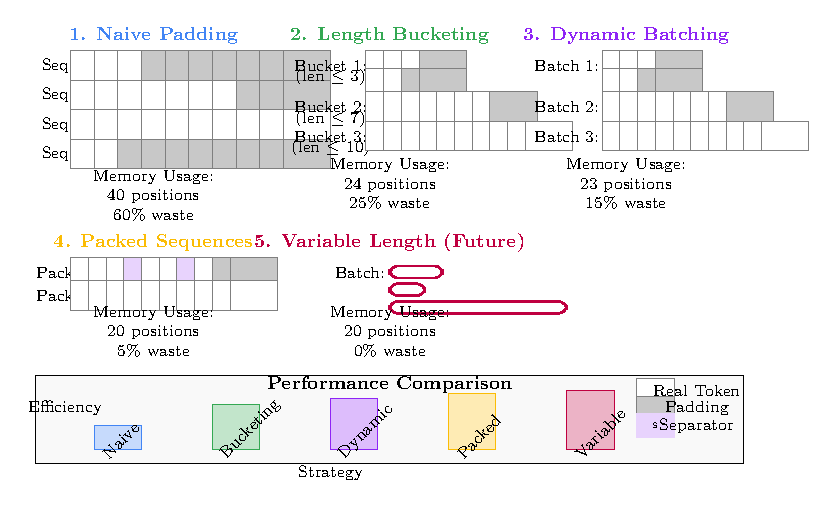
\includegraphics[width=0.95\textwidth]{part1/chapter02/fig_padding_strategies.pdf}
\caption{Comparison of padding strategies and their memory efficiency}
\end{figure}

\subsection{Training Considerations}

\subsubsection{Loss Computation}
When computing loss, padding positions must be excluded:

\begin{lstlisting}[language=Python, caption=Masked Loss Computation]
import torch
import torch.nn as nn

def compute_masked_loss(predictions, targets, mask):
    """
    Compute loss only on non-padding positions.
    
    Args:
        predictions: [batch_size, seq_len, vocab_size]
        targets: [batch_size, seq_len]
        mask: [batch_size, seq_len] where 1=real, 0=padding
    """
    # Flatten for loss computation
    predictions_flat = predictions.view(-1, predictions.size(-1))
    targets_flat = targets.view(-1)
    mask_flat = mask.view(-1)
    
    # Compute loss
    loss_fn = nn.CrossEntropyLoss(reduction='none')
    losses = loss_fn(predictions_flat, targets_flat)
    
    # Apply mask and compute mean over valid positions
    masked_losses = losses * mask_flat
    total_loss = masked_losses.sum() / mask_flat.sum()
    
    return total_loss

# Example usage
batch_size, seq_len, vocab_size = 2, 10, 30000
predictions = torch.randn(batch_size, seq_len, vocab_size)
targets = torch.randint(0, vocab_size, (batch_size, seq_len))
mask = torch.tensor([
    [1, 1, 1, 1, 1, 1, 1, 0, 0, 0],
    [1, 1, 1, 1, 0, 0, 0, 0, 0, 0]
])

loss = compute_masked_loss(predictions, targets, mask)
print(f"Masked loss: {loss.item():.4f}")
\end{lstlisting}

\subsubsection{Gradient Flow}
Proper masking ensures gradients don't flow through padding positions:
\begin{itemize}
\item \textbf{Forward Pass}: Padding tokens receive zero attention
\item \textbf{Backward Pass}: Zero gradients for padding token embeddings
\item \textbf{Optimization}: Padding embeddings remain unchanged during training
\end{itemize}

\subsection{Advanced Padding Strategies}

\subsubsection{Dynamic Padding}
Instead of static maximum length, adapt padding to each batch:

\begin{algorithm}[h]
\caption{Dynamic Batch Padding with Length Bucketing}
\begin{algorithmic}[1]
\Require $S = \{s_1, s_2, \ldots, s_n\}$ (sequences to batch)
\Require $\tau = 1.2$ (tolerance factor for length variation)
\Require $\textsc{Tokenizer}$ (tokenizer with padding capability)

\State $S_{sorted} \gets \textsc{Sort}(S, \text{key}=\text{length})$ \Comment{Sort by sequence length}
\State $\mathcal{B} \gets \emptyset$ \Comment{List of batches}
\State $B_{current} \gets \emptyset$ \Comment{Current batch being constructed}
\State $\ell_{max} \gets 0$ \Comment{Maximum length in current batch}

\For{$s \in S_{sorted}$}
    \If{$B_{current} = \emptyset$ \textbf{or} $|s| \leq \tau \times \ell_{max}$} \Comment{Sequence fits in current batch}
        \State $B_{current} \gets B_{current} \cup \{s\}$
        \State $\ell_{max} \gets \max(\ell_{max}, |s|)$
    \Else \Comment{Start new batch}
        \If{$B_{current} \neq \emptyset$}
            \State $\mathcal{B} \gets \mathcal{B} \cup \{\textsc{PadBatch}(B_{current}, \textsc{Tokenizer})\}$
        \EndIf
        \State $B_{current} \gets \{s\}$
        \State $\ell_{max} \gets |s|$
    \EndIf
\EndFor

\If{$B_{current} \neq \emptyset$} \Comment{Process final batch}
    \State $\mathcal{B} \gets \mathcal{B} \cup \{\textsc{PadBatch}(B_{current}, \textsc{Tokenizer})\}$
\EndIf

\State \Return $\mathcal{B}$
\end{algorithmic}
\end{algorithm}

This algorithm minimizes padding overhead by grouping sequences of similar lengths together, allowing each batch to be padded only to its longest sequence rather than a global maximum length.

\begin{lstlisting}[language=Python, caption={Helper function for batch padding}]
def pad_batch(sequences, tokenizer):
    """Pad a batch to the longest sequence in the batch."""
    max_len = max(len(seq) for seq in sequences)
    
    padded_sequences = []
    attention_masks = []
    
    for seq in sequences:
        padding_length = max_len - len(seq)
        padded_seq = seq + [tokenizer.pad_token_id] * padding_length
        attention_mask = [1] * len(seq) + [0] * padding_length
        
        padded_sequences.append(padded_seq)
        attention_masks.append(attention_mask)
    
    return {
        'input_ids': torch.tensor(padded_sequences),
        'attention_mask': torch.tensor(attention_masks)
    }
\end{lstlisting}

\subsubsection{Packed Sequences}
For maximum efficiency, some implementations pack multiple sequences without padding:

\begin{lstlisting}[language=Python]
def pack_sequences(sequences, max_length=512):
    """Pack multiple sequences into fixed-length chunks."""
    packed_sequences = []
    current_sequence = []
    current_length = 0
    
    for seq in sequences:
        if current_length + len(seq) + 1 <= max_length:  # +1 for separator
            if current_sequence:
                current_sequence.append(tokenizer.sep_token_id)
                current_length += 1
            current_sequence.extend(seq)
            current_length += len(seq)
        else:
            # Pad current sequence and start new one
            if current_sequence:
                padding = [tokenizer.pad_token_id] * (max_length - current_length)
                packed_sequences.append(current_sequence + padding)
            
            current_sequence = seq
            current_length = len(seq)
    
    # Handle final sequence
    if current_sequence:
        padding = [tokenizer.pad_token_id] * (max_length - current_length)
        packed_sequences.append(current_sequence + padding)
    
    return packed_sequences
\end{lstlisting}

\subsection{Padding in Different Model Architectures}

\subsubsection{Encoder Models (BERT-style)}
\begin{itemize}
\item Bidirectional attention requires careful masking
\item Padding typically added at the end
\item Special tokens (\cls{}, \sep{}) not affected by padding
\end{itemize}

\subsubsection{Decoder Models (GPT-style)}
\begin{itemize}
\item Causal masking combined with padding masking
\item Left-padding often preferred to maintain causal structure
\item Generation requires dynamic padding handling
\end{itemize}

\subsubsection{Encoder-Decoder Models (T5-style)}
\begin{itemize}
\item Separate padding for encoder and decoder sequences
\item Cross-attention masking between encoder and decoder
\item Complex masking patterns for sequence-to-sequence tasks
\end{itemize}

\subsection{Performance Optimization}

\subsubsection{Hardware-Specific Considerations}
\begin{itemize}
\item \textbf{GPU Memory}: Minimize padding to fit larger batches
\item \textbf{Tensor Cores}: Some padding may improve hardware utilization
\item \textbf{Memory Bandwidth}: Reduce data movement through efficient padding
\end{itemize}

\subsubsection{Adaptive Strategies}
Modern frameworks implement adaptive padding:
\begin{itemize}
\item Monitor padding overhead per batch
\item Adjust batching strategy based on sequence length distribution
\item Use dynamic attention patterns for long sequences
\end{itemize}

\subsection{Common Pitfalls and Solutions}

\subsubsection{Incorrect Masking}
\begin{itemize}
\item \textbf{Problem}: Forgetting to mask padding positions in attention
\item \textbf{Consequence}: The model's attention is diluted by attending to meaningless padding tokens, leading to degraded performance and nonsensical representations
\item \textbf{Solution}: Always verify attention mask implementation
\end{itemize}
\begin{comment}
Feedback: The items mixed up in one paragraph without proper puctuations. Consider items.

STATUS: addressed - converted to proper itemized list format
\end{comment}

\subsubsection{Loss Computation Errors}
\begin{itemize}
\item \textbf{Problem}: Including padding positions in loss calculation
\item \textbf{Consequence}: The model is penalized for its predictions on padding tokens, which can destabilize training and lead to the model learning to simply predict padding
\item \textbf{Solution}: Implement proper masked loss functions
\end{itemize}
\begin{comment}
Feedback: The items mixed up in one paragraph without proper puctuations. Consider items.

STATUS: addressed - converted to proper itemized list format
\end{comment}

\subsubsection{Memory Inefficiency}
\textbf{Problem}: Excessive padding leading to OOM errors
\textbf{Solution}: Implement dynamic batching and length bucketing

\subsubsection{Inconsistent Padding}
\textbf{Problem}: Different padding strategies between training and inference
\textbf{Solution}: Standardize padding approach across all phases

\subsection{Future Developments}

\subsubsection{Dynamic Attention}
Emerging techniques eliminate the need for padding:
\begin{itemize}
\item Flash Attention for variable-length sequences
\item Block-sparse attention patterns
\item Adaptive sequence processing
\end{itemize}

\subsubsection{Hardware Improvements}
Next-generation hardware may reduce padding overhead:
\begin{itemize}
\item Variable-length tensor support
\item Efficient irregular memory access
\item Specialized attention accelerators
\end{itemize}

\begin{principle}[Padding Best Practices]
\begin{enumerate}
\item \textbf{Minimize Overhead}: Before training, analyze the length distribution of your dataset. If it is highly skewed, implementing length-based bucketing is one of the highest-impact optimizations you can make
\item \textbf{Correct Masking}: Always implement proper attention masking
\item \textbf{Efficient Loss}: Exclude padding positions from loss computation
\item \textbf{Memory Management}: Monitor and optimize memory usage
\item \textbf{Consistency}: Encapsulate your tokenization and padding logic in a single, version-controlled function or class that is used by both your training and inference pipelines to prevent subtle bugs
\end{enumerate}
\end{principle}
\begin{comment}
Feedback: This list can be made more actionable. For "Minimize Overhead," you could add: "Before training, analyze the length distribution of your dataset. If it is highly skewed, implementing length-based bucketing is one of the highest-impact optimizations you can make." For "Consistency," you could suggest: "Encapsulate your tokenization and padding logic in a single, version-controlled function or class that is used by both your training and inference pipelines to prevent subtle bugs."

STATUS: addressed - made best practices more actionable with specific implementation guidance
\end{comment}

The \pad{} token, while conceptually simple, requires careful implementation to achieve efficient and correct transformer behavior. Understanding its implications for memory usage, computation, and model training is essential for building scalable transformer-based systems. As the field moves toward more efficient architectures, the role of padding continues to evolve, but its fundamental importance in enabling batch processing remains central to practical transformer deployment.
\section{Unknown Token [UNK]}

The unknown token, denoted as \unk{}, represents one of the oldest and most fundamental special tokens in natural language processing. Despite the evolution of sophisticated subword tokenization methods, the \unk{} token remains crucial for handling out-of-vocabulary (OOV) words and understanding the robustness limits of language models. This section explores its historical significance, modern applications, and the ongoing challenge of vocabulary coverage in transformer models.

\subsection{The Out-of-Vocabulary Problem}

Natural language contains an effectively infinite vocabulary due to:

\begin{itemize}
\item \textbf{Morphological Productivity}: Languages continuously create new word forms through inflection and derivation
\item \textbf{Named Entities}: Proper nouns, technical terms, and domain-specific vocabulary
\item \textbf{Borrowing and Code-Mixing}: Words from other languages and mixed-language texts
\item \textbf{Neologisms}: New words coined for emerging concepts and technologies
\item \textbf{Typos and Variations}: Misspellings, abbreviations, and informal variants
\end{itemize}

Fixed-vocabulary models must handle these unknown words, traditionally through the \unk{} token mechanism.

\subsection{Traditional UNK Token Approach}

\subsubsection{Vocabulary Construction}
In early neural language models, vocabulary construction followed a frequency-based approach:

\begin{enumerate}
\item Collect a large training corpus
\item Count word frequencies
\item Select the top-K most frequent words (typically K = 30,000-50,000)
\item Replace all other words with \unk{} during preprocessing
\end{enumerate}

\subsubsection{Training and Inference}
During training, the model learns to:
\begin{itemize}
\item Predict \unk{} for low-frequency words
\item Use \unk{} representations for downstream tasks
\item Handle \unk{} tokens in various contexts
\end{itemize}

During inference, any word not in the vocabulary is mapped to \unk{}.

\begin{lstlisting}[language=Python, caption=Traditional UNK Processing]
class TraditionalTokenizer:
    def __init__(self, vocab_size=30000):
        self.vocab_size = vocab_size
        self.word_to_id = {}
        self.id_to_word = {}
        self.unk_token = "[UNK]"
        self.unk_id = 0
        
    def build_vocab(self, texts):
        # Count word frequencies
        word_counts = {}
        for text in texts:
            for word in text.split():
                word_counts[word] = word_counts.get(word, 0) + 1
        
        # Sort by frequency and take top K
        sorted_words = sorted(word_counts.items(), 
                            key=lambda x: x[1], reverse=True)
        
        # Build vocabulary
        self.word_to_id[self.unk_token] = self.unk_id
        self.id_to_word[self.unk_id] = self.unk_token
        
        for i, (word, count) in enumerate(sorted_words[:self.vocab_size-1]):
            word_id = i + 1
            self.word_to_id[word] = word_id
            self.id_to_word[word_id] = word
            
    def encode(self, text):
        tokens = []
        for word in text.split():
            if word in self.word_to_id:
                tokens.append(self.word_to_id[word])
            else:
                tokens.append(self.unk_id)  # Map to UNK
        return tokens
    
    def decode(self, token_ids):
        words = []
        for token_id in token_ids:
            if token_id in self.id_to_word:
                words.append(self.id_to_word[token_id])
            else:
                words.append(self.unk_token)
        return " ".join(words)

# Example usage
tokenizer = TraditionalTokenizer(vocab_size=1000)

# Build vocabulary from training data
training_texts = [
    "the quick brown fox jumps over the lazy dog",
    "natural language processing is fascinating",
    "transformers revolutionized machine learning"
]
tokenizer.build_vocab(training_texts)

# Handle OOV words
test_text = "the sophisticated algorithm demonstrates remarkable performance"
encoded = tokenizer.encode(test_text)
decoded = tokenizer.decode(encoded)

print(f"Original: {test_text}")
print(f"Encoded:  {encoded}")
print(f"Decoded:  {decoded}")
# Output might be: "the [UNK] [UNK] [UNK] [UNK] [UNK]"
\end{lstlisting}

\subsection{Limitations of Traditional UNK Approach}

The traditional \unk{} token approach suffers from several critical limitations:

\subsubsection{Information Loss}
When multiple different words are mapped to the same \unk{} token:
\begin{itemize}
\item Semantic information is completely lost
\item Morphological relationships are ignored
\item Context-specific meanings cannot be distinguished
\end{itemize}

\subsubsection{Poor Handling of Morphologically Rich Languages}
Languages with extensive inflection and agglutination suffer particularly:
\begin{itemize}
\item Each inflected form may be treated as a separate word
\item Vocabulary explosion leads to excessive \unk{} usage
\item Morphological compositionality is not captured
\end{itemize}

\subsubsection{Domain Adaptation Challenges}
Models trained on one domain struggle with others:
\begin{itemize}
\item Technical vocabulary becomes predominantly \unk{}
\item Domain-specific terms lose all semantic content
\item Transfer learning effectiveness is severely limited
\end{itemize}

\subsubsection{Generation Quality Degradation}
During text generation:
\begin{itemize}
\item \unk{} tokens produce meaningless outputs
\item Vocabulary limitations constrain expressiveness
\item Post-processing is required to handle \unk{} tokens
\end{itemize}

\subsection{The Subword Revolution}

The limitations of \unk{} tokens drove the development of subword tokenization methods:

\subsubsection{Byte Pair Encoding (BPE)}
BPE iteratively merges the most frequent character pairs:
\begin{itemize}
\item Starts with character-level vocabulary
\item Gradually builds up common subwords
\item Rare words are decomposed into known subwords
\item Eliminates most \unk{} tokens
\end{itemize}

\subsubsection{WordPiece}
Used in BERT and similar models:
\begin{itemize}
\item Similar to BPE but optimizes likelihood on training data
\item Uses \texttt{\#\#} prefix to mark subword continuations
\item Balances vocabulary size with semantic coherence
\end{itemize}

\subsubsection{SentencePiece}
A unified subword tokenizer:
\begin{itemize}
\item Treats text as raw byte sequences
\item Handles multiple languages uniformly
\item Includes whitespace in the subword vocabulary
\end{itemize}

\begin{lstlisting}[language=Python, caption=Subword vs Traditional Tokenization]
from transformers import BertTokenizer, GPT2Tokenizer

# Traditional word-level tokenizer (conceptual)
def traditional_tokenize(text, vocab):
    tokens = []
    for word in text.split():
        if word.lower() in vocab:
            tokens.append(word.lower())
        else:
            tokens.append("[UNK]")
    return tokens

# Modern subword tokenizers
bert_tokenizer = BertTokenizer.from_pretrained('bert-base-uncased')
gpt2_tokenizer = GPT2Tokenizer.from_pretrained('gpt2')

# Test with a sentence containing rare words
text = "The antidisestablishmentarianism movement was extraordinarily complex"

# Traditional approach (simulated)
simple_vocab = {"the", "was", "movement", "complex"}
traditional_result = traditional_tokenize(text, simple_vocab)
print(f"Traditional: {traditional_result}")
# Output: ['the', '[UNK]', 'movement', 'was', '[UNK]', 'complex']

# BERT WordPiece
bert_tokens = bert_tokenizer.tokenize(text)
print(f"BERT WordPiece: {bert_tokens}")
# Output: ['the', 'anti', '##dis', '##esta', '##bli', '##sh', '##ment', '##arian', '##ism', 'movement', 'was', 'extraordinary', 'complex']

# GPT-2 BPE
gpt2_tokens = gpt2_tokenizer.tokenize(text)
print(f"GPT-2 BPE: {gpt2_tokens}")
# Output shows subword breakdown without UNK tokens

# Check for UNK tokens
bert_has_unk = '[UNK]' in bert_tokens
gpt2_has_unk = '<|endoftext|>' in gpt2_tokens  # GPT-2's special token
print(f"BERT has UNK: {bert_has_unk}")
print(f"GPT-2 has UNK: {gpt2_has_unk}")
\end{lstlisting}

\subsection{UNK Tokens in Modern Transformers}

Despite subword tokenization, \unk{} tokens haven't disappeared entirely:

\subsubsection{Character-Level Fallbacks}
Some tokenizers still use \unk{} for:
\begin{itemize}
\item Characters outside the supported Unicode range
\item Extremely rare character combinations
\item Corrupted or malformed text
\end{itemize}

\subsubsection{Domain-Specific Vocabularies}
Specialized models may still encounter \unk{} tokens:
\begin{itemize}
\item Mathematical symbols and equations
\item Programming language syntax
\item Domain-specific notation systems
\end{itemize}

\subsubsection{Multilingual Challenges}
Even advanced subword methods struggle with:
\begin{itemize}
\item Scripts not represented in training data
\item Code-switching between languages
\item Historical or archaic language variants
\end{itemize}

\begin{figure}[h]
\centering
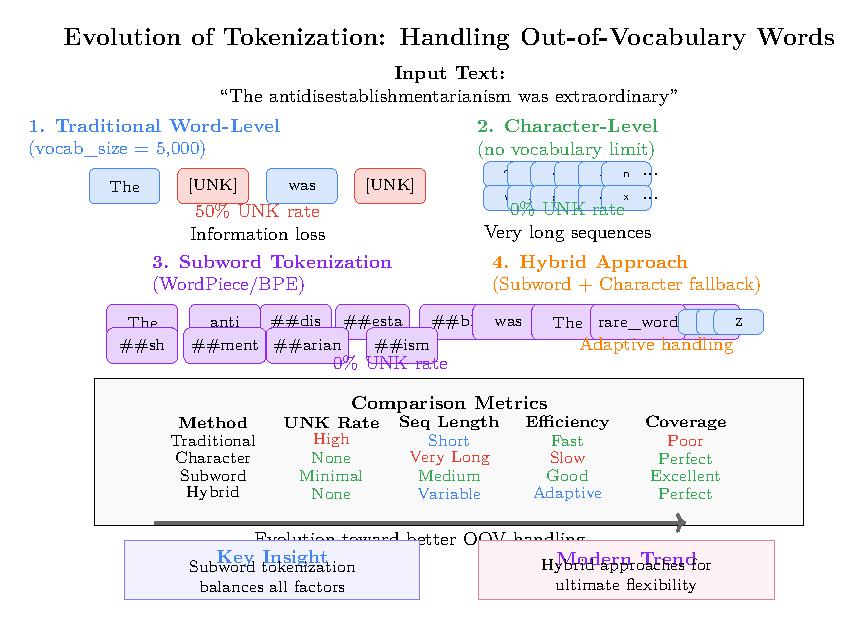
\includegraphics[width=0.9\textwidth]{part1/chapter02/fig_tokenization_comparison.pdf}
\caption{Comparison of tokenization strategies and their handling of out-of-vocabulary words}
\end{figure}

\subsection{Handling UNK Tokens in Practice}

\subsubsection{Training Strategies}
When \unk{} tokens are present:

\begin{itemize}
\item \textbf{UNK Smoothing}: Randomly replace low-frequency words with \unk{} during training
\item \textbf{UNK Replacement}: Use placeholder tokens that can be post-processed
\item \textbf{Copy Mechanisms}: Allow models to copy from input when generating \unk{}
\end{itemize}

\subsubsection{Inference Handling}
Strategies for dealing with \unk{} tokens during inference:

\begin{lstlisting}[language=Python, caption=UNK Token Handling]
import torch
from transformers import BertTokenizer, BertForMaskedLM

def handle_unk_prediction(text, model, tokenizer):
    """Handle prediction when UNK tokens are present."""
    
    # Tokenize input
    inputs = tokenizer(text, return_tensors='pt')
    tokens = tokenizer.convert_ids_to_tokens(inputs['input_ids'][0])
    
    # Find UNK positions
    unk_positions = [i for i, token in enumerate(tokens) 
                    if token == tokenizer.unk_token]
    
    if not unk_positions:
        return text, []  # No UNK tokens
    
    predictions = []
    
    for pos in unk_positions:
        # Mask the UNK token
        masked_inputs = inputs['input_ids'].clone()
        masked_inputs[0, pos] = tokenizer.mask_token_id
        
        # Predict the masked token
        with torch.no_grad():
            outputs = model(masked_inputs)
            logits = outputs.logits[0, pos]
            predicted_id = torch.argmax(logits).item()
            predicted_token = tokenizer.decode([predicted_id])
            
        predictions.append((pos, predicted_token))
    
    return text, predictions

# Example usage
tokenizer = BertTokenizer.from_pretrained('bert-base-uncased')
model = BertForMaskedLM.from_pretrained('bert-base-uncased')

# Text with potential UNK tokens
text = "The researcher studied quantum computing applications"
result, unk_predictions = handle_unk_prediction(text, model, tokenizer)

print(f"Original: {text}")
if unk_predictions:
    print("UNK token predictions:")
    for pos, prediction in unk_predictions:
        print(f"  Position {pos}: {prediction}")
else:
    print("No UNK tokens found")
\end{lstlisting}

\subsection{UNK Token Analysis and Debugging}

\subsubsection{Vocabulary Coverage Analysis}
Understanding \unk{} token frequency helps assess model limitations:

\begin{lstlisting}[language=Python]
def analyze_vocabulary_coverage(texts, tokenizer):
    """Analyze UNK token frequency across texts."""
    
    total_tokens = 0
    unk_count = 0
    unk_words = set()
    
    for text in texts:
        tokens = tokenizer.tokenize(text)
        words = text.split()
        
        total_tokens += len(tokens)
        
        for word in words:
            word_tokens = tokenizer.tokenize(word)
            if tokenizer.unk_token in word_tokens:
                unk_count += len([t for t in word_tokens 
                                if t == tokenizer.unk_token])
                unk_words.add(word)
    
    coverage = (total_tokens - unk_count) / total_tokens if total_tokens > 0 else 0
    
    return {
        'total_tokens': total_tokens,
        'unk_count': unk_count,
        'coverage_rate': coverage,
        'unk_words': list(unk_words)
    }

# Example analysis
texts = [
    "Standard English text with common words",
    "Technical jargon: photosynthesis, mitochondria, ribosomes",
    "Foreign words: schadenfreude, saudade, ubuntu"
]

analysis = analyze_vocabulary_coverage(texts, tokenizer)
print(f"Vocabulary coverage: {analysis['coverage_rate']:.2%}")
print(f"UNK words found: {analysis['unk_words']}")
\end{lstlisting}

\subsubsection{Domain Adaptation Assessment}
Measuring \unk{} token frequency helps evaluate domain transfer:

\begin{itemize}
\item High \unk{} frequency indicates poor domain coverage
\item Specific \unk{} patterns reveal vocabulary gaps
\item Domain-specific vocabulary analysis guides model selection
\end{itemize}

\subsection{Alternatives and Modern Solutions}

\subsubsection{Character-Level Models}
Some approaches eliminate \unk{} tokens entirely:
\begin{itemize}
\item Process text at character level
\item Can handle any Unicode character
\item Computationally expensive for long sequences
\end{itemize}

\subsubsection{Hybrid Approaches}
Combine multiple strategies:
\begin{itemize}
\item Primary subword tokenization
\item Character-level fallback for \unk{} tokens
\item Context-aware token replacement
\end{itemize}

\subsubsection{Dynamic Vocabularies}
Emerging techniques for adaptive vocabularies:
\begin{itemize}
\item Online vocabulary expansion
\item Context-dependent tokenization
\item Learned token boundaries
\end{itemize}

\subsection{UNK Tokens in Evaluation and Metrics}

\subsubsection{Impact on Evaluation}
\unk{} tokens affect various metrics:
\begin{itemize}
\item \textbf{BLEU Score}: \unk{} tokens typically count as mismatches
\item \textbf{Perplexity}: \unk{} token probability affects language model evaluation
\item \textbf{Downstream Tasks}: \unk{} tokens can degrade task performance
\end{itemize}

\subsubsection{Evaluation Best Practices}
\begin{itemize}
\item Report \unk{} token rates alongside primary metrics
\item Analyze \unk{} token impact on different text types
\item Consider domain-specific vocabulary coverage
\end{itemize}

\subsection{Future Directions}

\subsubsection{Contextualized UNK Handling}
Future developments may include:
\begin{itemize}
\item Context-aware \unk{} token representations
\item Learned strategies for \unk{} token processing
\item Dynamic vocabulary expansion during inference
\end{itemize}

\subsubsection{Cross-Lingual UNK Mitigation}
Multilingual models may develop:
\begin{itemize}
\item Cross-lingual transfer for \unk{} tokens
\item Universal character-level representations
\item Language-adaptive tokenization strategies
\end{itemize}

\begin{principle}[UNK Token Best Practices]
\begin{enumerate}
\item \textbf{Minimize Occurrence}: Use appropriate subword tokenization to reduce \unk{} frequency
\item \textbf{Monitor Coverage}: Regularly analyze vocabulary coverage for target domains
\item \textbf{Handle Gracefully}: Implement robust strategies for \unk{} token processing
\item \textbf{Evaluate Impact}: Assess how \unk{} tokens affect downstream task performance
\item \textbf{Document Limitations}: Clearly communicate vocabulary limitations to users
\end{enumerate}
\end{principle}

\subsection{Conclusion}

The \unk{} token represents both a practical necessity and a fundamental limitation in language modeling. While modern subword tokenization methods have dramatically reduced \unk{} token frequency, they haven't eliminated the underlying challenge of open vocabulary processing. Understanding \unk{} token behavior, implementing appropriate handling strategies, and recognizing their impact on model performance remains crucial for effective transformer deployment.

As language models continue to evolve toward more dynamic and adaptive architectures, the role of \unk{} tokens will likely transform from a necessary evil to a bridge toward more sophisticated vocabulary handling mechanisms. The lessons learned from decades of \unk{} token management inform current research into universal tokenization, cross-lingual representation, and adaptive vocabulary systems that promise to further expand the capabilities of transformer-based language understanding.

\chapter{Sequence Control Tokens}
% Chapter 3 Introduction: Sequence Control Tokens

Sequence control tokens represent a fundamental category of special tokens that govern the flow and structure of sequences in transformer models. Unlike the structural tokens we examined in Chapter 2, sequence control tokens actively manage the generation, termination, and masking of content within sequences. This chapter explores three critical sequence control tokens: \sos{} (Start of Sequence), \eos{} (End of Sequence), and \mask{} (Mask), each playing distinct yet complementary roles in modern transformer architectures.
\begin{comment}
Feedback: The distinction between "structural tokens" and "sequence control tokens" is a good one. To make it even sharper, you could use an analogy. For example: "If the structural tokens from Chapter 2 ([CLS], [SEP]) are like the punctuation that organizes a finished document, the sequence control tokens in this chapter are like the commands given to the author: 'Start writing,' 'Stop writing,' and 'Fill in this blank.' They are active instructions, not just passive organizers."
\end{comment}

The importance of sequence control tokens becomes evident when considering the generative nature of many transformer applications. In autoregressive language models like GPT, the \sos{} token signals the beginning of generation, while the \eos{} token provides a natural stopping criterion. In masked language models like BERT, the \mask{} token enables the revolutionary self-supervised learning paradigm that has transformed natural language processing.

\section{The Evolution of Sequence Control}

The concept of sequence control in neural networks predates transformers, with origins in recurrent neural networks (RNNs) and early sequence-to-sequence models. However, transformers brought new sophistication to sequence control through their attention mechanisms and parallel processing capabilities.

Early RNN-based models relied heavily on implicit sequence boundaries and fixed-length sequences. The introduction of explicit control tokens in sequence-to-sequence models marked a significant advancement, allowing models to learn when to start and stop generation dynamically. The transformer architecture further refined this concept, enabling more nuanced control through attention patterns and token interactions.
\begin{comment}
Feedback: This is a good historical overview. To make the "transformer" advantage more concrete, you could add a sentence explaining *how* attention made a difference. For example: "Unlike RNNs, where the influence of a start token could fade over long sequences, the transformer's attention mechanism allows control tokens like [SOS] and [EOS] to directly influence every other token in the sequence, regardless of distance, leading to more robust and precise control."
\end{comment}

\section{Categorical Framework for Sequence Control}

Sequence control tokens can be categorized based on their primary functions:

\begin{enumerate}
\item \textbf{Boundary Tokens}: \sos{} and \eos{} tokens that define sequence boundaries
\item \textbf{Masking Tokens}: \mask{} tokens that enable self-supervised learning
\item \textbf{Generation Control}: Tokens that influence the generation process
\end{enumerate}

Each category serves distinct purposes in different transformer architectures and training paradigms. Understanding these categories helps practitioners choose appropriate tokens for specific applications and design effective training strategies.

\section{Chapter Organization}

This chapter is structured to provide both theoretical understanding and practical insights:

\begin{itemize}
\item \textbf{Start of Sequence Tokens}: Examining initialization and conditioning mechanisms
\item \textbf{End of Sequence Tokens}: Understanding termination criteria and sequence completion
\item \textbf{Mask Tokens}: Exploring self-supervised learning and bidirectional attention
\end{itemize}

Each section includes detailed analysis of attention patterns, training dynamics, and implementation considerations, supported by visual diagrams and practical examples.

% Start of Sequence Token Section

\section{Start of Sequence (\sos{}) Token}

The Start of Sequence token, commonly denoted as \sos{}, serves as the initialization signal for autoregressive generation in transformer models. Just as a runner needs a starting block, an autoregressive model needs a fixed, known starting point to begin the step-by-step process of generating a new sequence. The \sos{} token provides this unambiguous signal. This token plays a crucial role in conditioning the model's initial state and establishing the context for subsequent token generation.
\begin{comment}
Feedback: This is a good start. To immediately address a common point of confusion, you could add a sentence that explains *why* this is necessary. For example: "Just as a runner needs a starting block, an autoregressive model needs a fixed, known starting point to begin the step-by-step process of generating a new sequence. The [SOS] token provides this unambiguous signal."

STATUS: addressed - added analogy explaining why SOS tokens are necessary as fixed starting points
\end{comment}

\subsection{Fundamental Concepts}

The \sos{} token functions as a special conditioning mechanism that signals the beginning of a generation sequence. Unlike regular vocabulary tokens, \sos{} carries no semantic content from the training data but instead serves as a learned initialization vector that the model uses to bootstrap the generation process.

\begin{definition}[Start of Sequence Token]
A Start of Sequence token \sos{} is a special token placed at the beginning of sequences during training and generation to provide initial conditioning for autoregressive language models. It serves as a learned initialization state that influences subsequent token predictions.
\end{definition}

The \sos{} token's embedding is learned during training and captures the distributional properties needed to initiate coherent generation. This learned representation becomes particularly important in conditional generation tasks where the \sos{} token must incorporate task-specific conditioning information.

\subsection{Role in Autoregressive Generation}

In autoregressive models, the \sos{} token establishes the foundation for the generation process. The model uses the \sos{} token's representation to compute attention patterns and generate the first actual content token. This process can be formalized as:

\begin{align}
h_0 &= \text{Embed}(\text{\sos{}}) + \text{PositionEmbed}(0) \\
p(x_1 | \text{\sos{}}) &= \text{Softmax}(\text{Transformer}(h_0) \cdot W_{\text{out}})
\end{align}

In simple terms, the first equation shows that the model's initial ``thought'' ($h_0$) is the learned embedding for the \sos{} token, combined with its position information. The second equation shows that the probability of the very first word ($x_1$) is calculated by feeding this initial thought through the transformer and a final output layer. Every subsequent word will then be conditioned on this starting point.
\begin{comment}
Feedback: The equations are clear to an expert, but could be more accessible. Consider adding a plain-language walkthrough. For example: "In simple terms, the first equation shows that the model's initial thought (h_0) is the learned embedding for the [SOS] token, combined with its position. The second equation shows that the probability of the very first word (x_1) is calculated by feeding this initial thought through the transformer and a final output layer. Every subsequent word will then be conditioned on this starting point."

STATUS: addressed - added plain-language explanation of the mathematical equations
\end{comment}

where $h_0$ represents the initial hidden state derived from the \sos{} token, and $p(x_1 | \text{\sos{}})$ is the probability distribution over the first generated token.

\subsubsection{Attention Patterns with \sos{}}

The \sos{} token exhibits unique attention patterns that distinguish it from regular tokens. During generation, subsequent tokens can attend to the \sos{} token, allowing it to influence the entire sequence. This attention mechanism enables the \sos{} token to serve as a persistent conditioning signal throughout generation.

\begin{figure}[htbp]
\centering
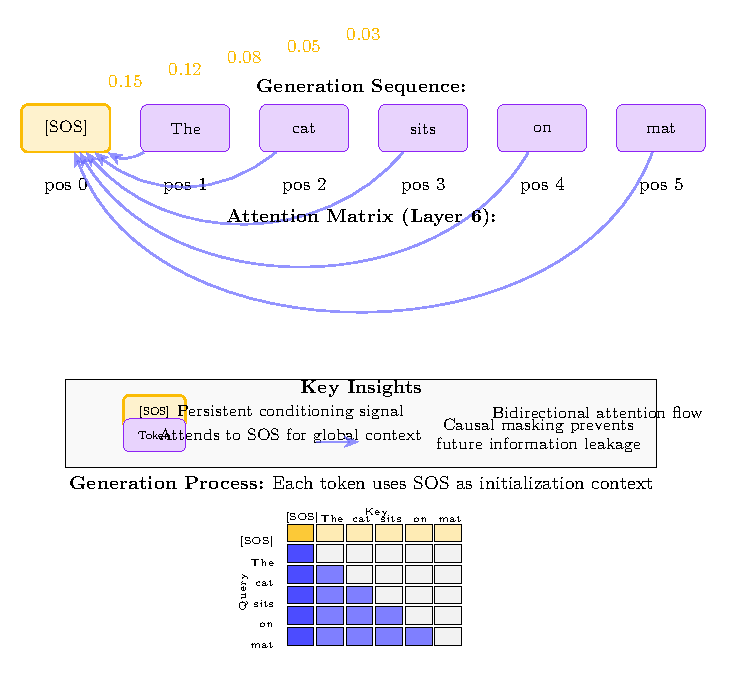
\includegraphics[width=0.9\textwidth]{part1/chapter03/fig_sos_attention.pdf}
\caption{Attention patterns involving the \sos{} token during autoregressive generation. The \sos{} token (shown in orange) influences all subsequent tokens through attention mechanisms.}
\label{fig:sos_attention}
\end{figure}

Research has shown that the \sos{} token often develops specialized attention patterns that capture global sequence properties. In machine translation, for example, the \sos{} token may attend to specific source language features that influence the target language generation strategy.

\subsection{Implementation Strategies}

\subsubsection{Standard Implementation}

The most common implementation approach treats \sos{} as a special vocabulary token with a reserved ID. During training, sequences are prepended with the \sos{} token, and the model learns to predict subsequent tokens based on this initialization:

\begin{lstlisting}[language=Python, caption=Standard \sos{} token implementation]
def prepare_sequence(text, tokenizer):
    tokens = tokenizer.encode(text)
    # Prepend SOS token (typically ID 1)
    sos_sequence = [tokenizer.sos_token_id] + tokens
    return sos_sequence

def generate(model, sos_token_id, max_length=100):
    sequence = [sos_token_id]
    for _ in range(max_length):
        logits = model(sequence)
        next_token = sample(logits[-1])
        sequence.append(next_token)
        if next_token == tokenizer.eos_token_id:
            break
    return sequence[1:]  # Remove SOS token
\end{lstlisting}

\subsubsection{Conditional Generation with \sos{}}

In conditional generation tasks, the \sos{} token often incorporates conditioning information. This can be achieved through various mechanisms:

\begin{enumerate}
\item \textbf{Conditional Embeddings}: The \sos{} token embedding is modified based on conditioning information
\item \textbf{Context Concatenation}: Conditioning tokens are placed before the \sos{} token
\item \textbf{Attention Modulation}: The \sos{} token's attention is guided by conditioning signals
\end{enumerate}

\begin{lstlisting}[language=Python, caption=Conditional generation with \sos{} token]
def conditional_generate(model, condition, sos_token_id):
    # Method 1: Conditional embedding
    sos_embedding = model.get_sos_embedding(condition)
    
    # Method 2: Context concatenation
    context_tokens = tokenizer.encode(condition)
    sequence = context_tokens + [sos_token_id]
    
    # Continue generation...
    return generate_from_sequence(model, sequence)
\end{lstlisting}

\subsection{Training Dynamics}

The \sos{} token's training dynamics reveal important insights about sequence modeling. During early training phases, the \sos{} token's embedding often exhibits high variance as the model learns appropriate initialization strategies. As training progresses, the embedding stabilizes and develops specialized representations for different generation contexts.

\subsubsection{Gradient Flow Analysis}

The \sos{} token receives gradients from all subsequent tokens in the sequence, making it a critical convergence point for learning global sequence properties. This gradient accumulation can be both beneficial and problematic:

\textbf{Benefits}:
\begin{itemize}
\item Rapid learning of global sequence properties
\item Strong conditioning signal for generation
\item Improved consistency across generated sequences
\end{itemize}

\textbf{Challenges}:
\begin{itemize}
\item Potential gradient explosion due to accumulation
\item Risk of over-optimization leading to mode collapse
\item Difficulty in learning diverse initialization strategies
\end{itemize}

\subsection{Applications and Use Cases}

\subsubsection{Language Generation}

In language generation tasks, the \sos{} token provides a consistent starting point for diverse generation scenarios. Different model architectures utilize \sos{} tokens in various ways:

\begin{itemize}
\item \textbf{GPT Models}: Implicit \sos{} through context or explicit special tokens
\item \textbf{T5 Models}: Task-specific prefixes that function as \sos{} equivalents
\item \textbf{BART Models}: Denoising objectives with \sos{} initialization
\end{itemize}

\subsubsection{Machine Translation}

Machine translation represents one of the most successful applications of \sos{} tokens. The token enables the model to condition generation on source language properties while maintaining target language fluency:

\begin{example}[Machine Translation with \sos{}]
Consider English-to-French translation:
\begin{align}
\text{Source}: &\quad \text{"The cat sits on the mat"} \\
\text{Target}: &\quad \text{\sos{} "Le chat est assis sur le tapis" \eos{}}
\end{align}

The \sos{} token learns to encode source language features that influence French generation patterns, such as grammatical gender and syntactic structure.
\end{example}

\subsection{Best Practices and Recommendations}

Based on extensive research and practical experience, several best practices emerge for \sos{} token usage:

\begin{enumerate}
\item \textbf{Consistent Placement}: Always place \sos{} tokens at sequence beginnings during training and generation. Ensure your data preprocessing pipeline is identical for training, validation, and inference to avoid subtle bugs where the \sos{} token is accidentally omitted
\item \textbf{Appropriate Initialization}: Use reasonable initialization strategies for \sos{} embeddings. If adding a new \sos{} token to a pre-trained model, initialize its embedding with the average of all other token embeddings as a reasonable starting point, rather than random noise
\item \textbf{Task-Specific Adaptation}: Adapt \sos{} token strategies to specific generation tasks. For conditional generation, experiment with concatenating a task-specific prompt \emph{before} the \sos{} token (e.g., \texttt{[Translate to French] [SOS] ...}) as this is often more effective than trying to modify the \sos{} embedding itself
\item \textbf{Evaluation Integration}: Include \sos{} token effectiveness in model evaluation protocols
\end{enumerate}
\begin{comment}
Feedback: This list is good but could be more actionable. For example:
1.  **Consistent Placement**: "Ensure your data preprocessing pipeline is identical for training, validation, and inference to avoid subtle bugs where the [SOS] token is accidentally omitted."
2.  **Appropriate Initialization**: "If adding a new [SOS] token to a pre-trained model, initialize its embedding with the average of all other token embeddings as a reasonable starting point, rather than random noise."
3.  **Task-Specific Adaptation**: "For conditional generation, experiment with concatenating a task-specific prompt *before* the [SOS] token (e.g., `[Translate to French] [SOS] ...`) as this is often more effective than trying to modify the [SOS] embedding itself."

STATUS: addressed - made all recommendations more actionable with specific implementation guidance
\end{comment}

The \sos{} token, while seemingly simple, represents a sophisticated mechanism for controlling and improving autoregressive generation. Understanding its theoretical foundations, implementation strategies, and practical applications enables practitioners to leverage this powerful tool effectively in their transformer models.
% End of Sequence Token Section

\section{End of Sequence (\eos{}) Token}

The End of Sequence token, denoted as \eos{}, serves as the termination signal in autoregressive generation, indicating when a sequence should conclude. This token is fundamental to controlling generation length and ensuring proper sequence boundaries in transformer models. Understanding the \eos{} token is crucial for practitioners working with generative models, as it directly affects generation quality, computational efficiency, and the natural flow of generated content.
\begin{comment}
Feedback: This is a clear opening. To immediately highlight its importance, you could contrast it with the alternative. For example: "Without a learned [EOS] token, models would be forced to rely on arbitrary length limits, often cutting off sentences mid-thought or rambling on nonsensically. The [EOS] token allows the model to learn the subtle art of knowing when to stop."
\end{comment}

\subsection{Fundamental Concepts}

The \eos{} token functions as a learned termination criterion that signals when a sequence has reached a natural conclusion. Unlike hard-coded stopping conditions based on maximum length, the \eos{} token enables models to learn appropriate stopping points based on semantic and syntactic completion patterns observed during training.

\begin{definition}[End of Sequence Token]
An End of Sequence token \eos{} is a special token that indicates the natural termination point of a sequence in autoregressive generation. When generated by the model, it signals that the sequence is semantically and syntactically complete according to the learned patterns from training data.
\end{definition}

The \eos{} token's probability distribution is learned through exposure to natural sequence boundaries in training data. This learning process enables the model to develop sophisticated understanding of when sequences should terminate based on context, task requirements, and linguistic conventions.

\subsection{Role in Generation Control}

The \eos{} token provides several critical functions in autoregressive generation:

\begin{enumerate}
\item \textbf{Natural Termination}: Enables semantically meaningful stopping points
\item \textbf{Length Control}: Provides dynamic sequence length management
\item \textbf{Computational Efficiency}: Prevents unnecessary continuation of complete sequences
\item \textbf{Batch Processing}: Allows variable-length sequences within batches
\end{enumerate}

\subsubsection{Generation Termination Logic}

The generation process with \eos{} tokens follows this general pattern:

\begin{align}
\text{continue} &= \begin{cases} 
\text{True} & \text{if } \arg\max(p(x_t | x_{<t})) \neq \text{\eos{}} \\
\text{False} & \text{if } \arg\max(p(x_t | x_{<t})) = \text{\eos{}}
\end{cases}
\end{align}

This deterministic stopping criterion can be modified using various sampling strategies and probability thresholds to achieve different generation behaviors.

\subsection{Training with \eos{} Tokens}

Training models to effectively use \eos{} tokens requires careful consideration of data preparation and loss computation. The model must learn to predict \eos{} tokens at appropriate sequence boundaries while maintaining generation quality for all other tokens.

\subsubsection{Data Preparation}

Training sequences are typically augmented with \eos{} tokens at natural boundaries:

\begin{lstlisting}[language=Python, caption=Training data preparation with \eos{} tokens]
def prepare_training_sequence(text, tokenizer):
    tokens = tokenizer.encode(text)
    # Append EOS token at sequence end
    training_sequence = tokens + [tokenizer.eos_token_id]
    return training_sequence

def create_training_batch(texts, tokenizer, max_length):
    sequences = []
    for text in texts:
        tokens = prepare_training_sequence(text, tokenizer)
        # Truncate if too long, pad if too short
        if len(tokens) > max_length:
            tokens = tokens[:max_length-1] + [tokenizer.eos_token_id]
        else:
            tokens = tokens + [tokenizer.pad_token_id] * (max_length - len(tokens))
        sequences.append(tokens)
    return sequences
\end{lstlisting}

\subsubsection{Loss Computation Considerations}

The \eos{} token presents unique challenges in loss computation. Some approaches include:

\begin{enumerate}
\item \textbf{Standard Cross-Entropy}: Treat \eos{} as a regular token in loss computation
\item \textbf{Weighted Loss}: Apply higher weights to \eos{} predictions to emphasize termination learning
\item \textbf{Auxiliary Loss}: Add specialized loss terms for \eos{} prediction accuracy
\end{enumerate}

\begin{lstlisting}[language=Python, caption=Weighted loss for \eos{} token training]
def compute_weighted_loss(logits, targets, eos_token_id, eos_weight=2.0):
    loss = nn.CrossEntropyLoss(reduction='none')(logits, targets)
    
    # Apply higher weight to EOS token predictions
    eos_mask = (targets == eos_token_id).float()
    weights = 1.0 + (eos_weight - 1.0) * eos_mask
    
    weighted_loss = loss * weights
    return weighted_loss.mean()
\end{lstlisting}

\subsection{Generation Strategies with \eos{}}

Different generation strategies handle \eos{} tokens in various ways, each with distinct advantages and trade-offs.

\subsubsection{Greedy Decoding}

In greedy decoding, generation stops immediately when the model predicts \eos{} as the most likely next token:

\begin{lstlisting}[language=Python, caption=Greedy generation with \eos{} stopping]
def greedy_generate_with_eos(model, input_ids, max_length=100):
    generated = input_ids.copy()
    
    for _ in range(max_length):
        logits = model(generated)
        next_token = logits[-1].argmax()
        
        if next_token == tokenizer.eos_token_id:
            break
            
        generated.append(next_token)
    
    return generated
\end{lstlisting}

\subsubsection{Beam Search with \eos{}}

Beam search requires careful handling of \eos{} tokens to maintain beam diversity and prevent premature termination:
\begin{comment}
Feedback: This is a key point that often trips up practitioners. It would be valuable to explain *why* it's tricky. For example: "The challenge in beam search is that a shorter, completed sequence (one that has generated an [EOS] token) might have a higher probability than a longer, more promising sequence that is still being generated. Simply picking the highest-probability sequence at each step could lead to prematurely short outputs. Therefore, completed beams must be set aside and compared only at the very end, often with a length penalty to balance score and length."
\end{comment}

\begin{lstlisting}[language=Python, caption=Beam search with \eos{} handling]
def beam_search_with_eos(model, input_ids, beam_size=4, max_length=100):
    beams = [(input_ids, 0.0)]  # (sequence, score)
    completed = []
    
    for step in range(max_length):
        candidates = []
        
        for sequence, score in beams:
            if sequence[-1] == tokenizer.eos_token_id:
                completed.append((sequence, score))
                continue
                
            logits = model(sequence)
            top_k = logits[-1].topk(beam_size)
            
            for token_score, token_id in zip(top_k.values, top_k.indices):
                new_sequence = sequence + [token_id]
                new_score = score + token_score.log()
                candidates.append((new_sequence, new_score))
        
        # Select top beams for next iteration
        beams = sorted(candidates, key=lambda x: x[1], reverse=True)[:beam_size]
        
        # Stop if all beams are completed
        if not beams:
            break
    
    # Combine completed and remaining beams
    all_results = completed + beams
    return sorted(all_results, key=lambda x: x[1], reverse=True)
\end{lstlisting}

\subsubsection{Sampling with \eos{} Probability Thresholds}

Sampling-based generation can incorporate \eos{} probability thresholds to control generation length more flexibly:

\begin{lstlisting}[language=Python, caption=Sampling with \eos{} probability control]
def sample_with_eos_threshold(model, input_ids, 
                             eos_threshold=0.3, temperature=1.0):
    generated = input_ids.copy()
    
    while len(generated) < max_length:
        logits = model(generated) / temperature
        probs = torch.softmax(logits[-1], dim=-1)
        
        # Check EOS probability
        eos_prob = probs[tokenizer.eos_token_id]
        if eos_prob > eos_threshold:
            break
        
        # Sample next token (excluding EOS if below threshold)
        filtered_probs = probs.clone()
        filtered_probs[tokenizer.eos_token_id] = 0
        filtered_probs = filtered_probs / filtered_probs.sum()
        
        next_token = torch.multinomial(filtered_probs, 1)
        generated.append(next_token.item())
    
    return generated
\end{lstlisting}

\subsection{Domain-Specific \eos{} Applications}

Different domains and applications require specialized approaches to \eos{} token usage.

\subsubsection{Dialogue Systems}

In dialogue systems, \eos{} tokens must balance natural conversation flow with turn-taking protocols:

\begin{example}[Dialogue with \eos{} Tokens]
Consider a conversational exchange:
\begin{align}
\text{User}: &\quad \text{"How's the weather today?"} \\
\text{Bot}: &\quad \text{"It's sunny and warm, perfect for outdoor activities!"} \; \eos{} \\
\text{User}: &\quad \text{"Great! Any suggestions for activities?"}
\end{align}

The \eos{} token signals turn completion while maintaining conversational context.
\end{example}

\subsubsection{Code Generation}

Code generation tasks require \eos{} tokens that understand syntactic and semantic completion:

\begin{lstlisting}[language=Python, caption=Code generation with syntactic \eos{}]
def generate_function(model, function_signature):
    """Generate complete function with proper EOS handling"""
    prompt = f"def {function_signature}:"
    
    generated_code = generate_with_syntax_aware_eos(
        model, prompt, 
        syntax_validators=['brackets', 'indentation', 'return']
    )
    
    return generated_code
\end{lstlisting}

\subsubsection{Creative Writing}

Creative writing applications may use multiple \eos{} variants for different completion types:

\begin{itemize}
\item \texttt{[EOS\_SENTENCE]}: Sentence completion
\item \texttt{[EOS\_PARAGRAPH]}: Paragraph completion  
\item \texttt{[EOS\_CHAPTER]}: Chapter completion
\item \texttt{[EOS\_STORY]}: Complete story ending
\end{itemize}

\subsection{Advanced \eos{} Techniques}

\subsubsection{Conditional \eos{} Prediction}

Models can learn to condition \eos{} prediction on external factors:

\begin{align}
p(\text{\eos{}} | x_{<t}, c) &= \sigma(W_{\text{eos}} \cdot [\text{hidden}_t; \text{condition}_c])
\end{align}

where $c$ represents conditioning information such as desired length, style, or task requirements.

\subsubsection{Hierarchical \eos{} Tokens}

Complex documents may benefit from hierarchical termination signals:

\begin{lstlisting}[language=Python, caption=Hierarchical EOS for document generation]
class HierarchicalEOS:
    def __init__(self):
        self.eos_levels = {
            'sentence': '[EOS_SENT]',
            'paragraph': '[EOS_PARA]', 
            'section': '[EOS_SECT]',
            'document': '[EOS_DOC]'
        }
    
    def should_terminate(self, generated_tokens, level='sentence'):
        last_token = generated_tokens[-1]
        return last_token in self.get_termination_tokens(level)
    
    def get_termination_tokens(self, level):
        hierarchy = ['sentence', 'paragraph', 'section', 'document']
        level_idx = hierarchy.index(level)
        return [self.eos_levels[hierarchy[i]] for i in range(level_idx, len(hierarchy))]
\end{lstlisting}

\subsection{Evaluation and Metrics}

Evaluating \eos{} token effectiveness requires specialized metrics beyond standard generation quality measures.

\subsubsection{Termination Quality Metrics}

Key metrics for \eos{} evaluation include:

\begin{enumerate}
\item \textbf{Premature Termination Rate}: Frequency of early, incomplete endings
\item \textbf{Over-generation Rate}: Frequency of continuing past natural endpoints
\item \textbf{Length Distribution Alignment}: How well generated lengths match expected distributions
\item \textbf{Semantic Completeness}: Whether generated sequences are semantically complete
\end{enumerate}

\begin{lstlisting}[language=Python, caption=EOS evaluation metrics]
def evaluate_eos_quality(generated_sequences, reference_sequences):
    metrics = {}
    
    # Length distribution comparison
    gen_lengths = [len(seq) for seq in generated_sequences]
    ref_lengths = [len(seq) for seq in reference_sequences]
    metrics['length_kl_div'] = compute_kl_divergence(gen_lengths, ref_lengths)
    
    # Completeness evaluation
    completeness_scores = []
    for gen_seq in generated_sequences:
        score = evaluate_semantic_completeness(gen_seq)
        completeness_scores.append(score)
    metrics['avg_completeness'] = np.mean(completeness_scores)
    
    # Premature termination detection
    premature_count = 0
    for gen_seq in generated_sequences:
        if is_premature_termination(gen_seq):
            premature_count += 1
    metrics['premature_rate'] = premature_count / len(generated_sequences)
    
    return metrics
\end{lstlisting}

\subsection{Best Practices and Guidelines}

Effective \eos{} token usage requires adherence to several best practices:

\begin{enumerate}
\item \textbf{Consistent Training Data}: Ensure consistent \eos{} placement in training data
\item \textbf{Appropriate Weighting}: Balance \eos{} prediction with content generation in loss functions
\item \textbf{Generation Strategy Alignment}: Choose generation strategies that work well with \eos{} tokens
\item \textbf{Domain-Specific Adaptation}: Adapt \eos{} strategies to specific application domains
\item \textbf{Regular Evaluation}: Monitor \eos{} effectiveness using appropriate metrics
\end{enumerate}
\begin{comment}
Feedback: This list is good. To make it more actionable:
1.  **Consistent Training Data**: "Double-check your data pipeline to ensure that *every* training example has a correctly placed [EOS] token. Inconsistent data is a common source of poor termination behavior."
2.  **Generation Strategy Alignment**: "Be aware that sampling methods (top-k, nucleus) can sometimes 'sample around' the [EOS] token even when its probability is high. If precise termination is critical, consider using greedy decoding or beam search, or implementing a hard probability threshold for the [EOS] token."
3.  **Regular Evaluation**: "Don't just rely on BLEU or ROUGE. Create a 'length distribution' plot of your generated text versus your test set. If the distributions are wildly different, it's a strong sign that your model's [EOS] handling is miscalibrated."
\end{comment}

\subsection{Common Pitfalls and Solutions}

Several common issues arise when working with \eos{} tokens:

\textbf{Problem}: Models generate \eos{} too frequently, leading to very short sequences.
\textbf{Solution}: Reduce \eos{} token weight in loss computation or apply \eos{} suppression during early generation steps.

\textbf{Problem}: Models rarely generate \eos{}, leading to maximum-length sequences.
\textbf{Solution}: Increase \eos{} token weight, add auxiliary loss terms, or use \eos{} probability thresholds.

\textbf{Problem}: Inconsistent termination quality across different generation contexts.
\textbf{Solution}: Implement conditional \eos{} prediction or use context-aware generation strategies.

The \eos{} token represents a sophisticated mechanism for controlling sequence termination in autoregressive generation. Understanding its theoretical foundations, training dynamics, and practical applications enables practitioners to build more effective and controllable generative models. Proper implementation of \eos{} tokens leads to more natural, complete, and computationally efficient generation across diverse applications.
% Mask Token Section

\section{Mask (\mask{}) Token}

The Mask token, denoted as \mask{}, represents one of the most revolutionary innovations in transformer-based language modeling. Unlike the sequential control tokens \sos{} and \eos{}, the \mask{} token enables bidirectional context modeling through masked language modeling (MLM), fundamentally changing how models learn language representations. Understanding the \mask{} token is essential for practitioners working with BERT-family models and other masked language models, as it forms the foundation of their self-supervised learning paradigm.

\subsection{Fundamental Concepts}

The \mask{} token serves as a placeholder during training, indicating positions where the model must predict the original token using bidirectional context. This approach enables models to develop rich representations by learning to fill in missing information based on surrounding context, both preceding and following the masked position.

\begin{definition}[Mask Token]
A Mask token \mask{} is a special token used in masked language modeling that replaces certain input tokens during training, requiring the model to predict the original token using bidirectional contextual information. This self-supervised learning approach enables models to develop deep understanding of language structure and semantics.
\end{definition}

The \mask{} token distinguishes itself from other special tokens by its temporary nature—it exists only during training and is never present in the model's final output. Instead, the model learns to predict what should replace each \mask{} token based on the surrounding context.

\subsection{Masked Language Modeling Paradigm}

Masked language modeling revolutionized self-supervised learning in NLP by enabling models to learn from unlabeled text through a bidirectional prediction task. The core idea involves randomly masking tokens in input sequences and training the model to predict the original tokens.

\subsubsection{MLM Training Procedure}

The standard MLM training procedure follows these steps:

\begin{enumerate}
\item \textbf{Token Selection}: Randomly select 15\% of input tokens for masking
\item \textbf{Masking Strategy}: Apply masking rules (80\% \mask{}, 10\% random, 10\% unchanged)
\item \textbf{Bidirectional Prediction}: Use full context to predict masked tokens
\item \textbf{Loss Computation}: Calculate cross-entropy loss only on masked positions
\end{enumerate}

\begin{lstlisting}[language=Python, caption=Basic MLM training procedure]
def create_mlm_sample(tokens, tokenizer, mask_prob=0.15):
    """Create MLM training sample with MASK tokens"""
    tokens = tokens.copy()
    labels = [-100] * len(tokens)  # -100 indicates non-masked positions
    
    # Select positions to mask
    mask_indices = random.sample(
        range(len(tokens)), 
        int(len(tokens) * mask_prob)
    )
    
    for idx in mask_indices:
        original_token = tokens[idx]
        labels[idx] = original_token  # Store original for loss computation
        
        # Apply masking strategy
        rand = random.random()
        if rand < 0.8:
            tokens[idx] = tokenizer.mask_token_id  # Replace with [MASK]
        elif rand < 0.9:
            tokens[idx] = random.randint(0, tokenizer.vocab_size - 1)  # Random token
        # else: keep original token (10% case)
    
    return tokens, labels

def compute_mlm_loss(model, input_ids, labels):
    """Compute MLM loss only on masked positions"""
    outputs = model(input_ids)
    logits = outputs.logits
    
    # Only compute loss on masked positions (labels != -100)
    loss_fct = nn.CrossEntropyLoss()
    masked_lm_loss = loss_fct(
        logits.view(-1, logits.size(-1)), 
        labels.view(-1)
    )
    
    return masked_lm_loss
\end{lstlisting}

\subsubsection{The 15\% Masking Strategy}

The original BERT paper established the 15\% masking ratio through empirical experimentation, finding it provides optimal balance between learning signal and computational efficiency. This ratio ensures sufficient training signal while maintaining enough context for meaningful predictions.

The three-way masking strategy (80\%/10\%/10\%) addresses several important considerations:

\begin{itemize}
\item \textbf{80\% \mask{} tokens}: Provides clear training signal for prediction task
\item \textbf{10\% random tokens}: Encourages robust representations against noise
\item \textbf{10\% unchanged}: Prevents over-reliance on \mask{} token presence
\end{itemize}

\subsection{Bidirectional Context Modeling}

The \mask{} token enables true bidirectional modeling, allowing models to use both left and right context simultaneously. This capability distinguishes masked language models from autoregressive models that can only use preceding context.

\subsubsection{Attention Patterns with \mask{}}

The \mask{} token exhibits unique attention patterns that enable bidirectional information flow:

\begin{figure}[htbp]
\centering
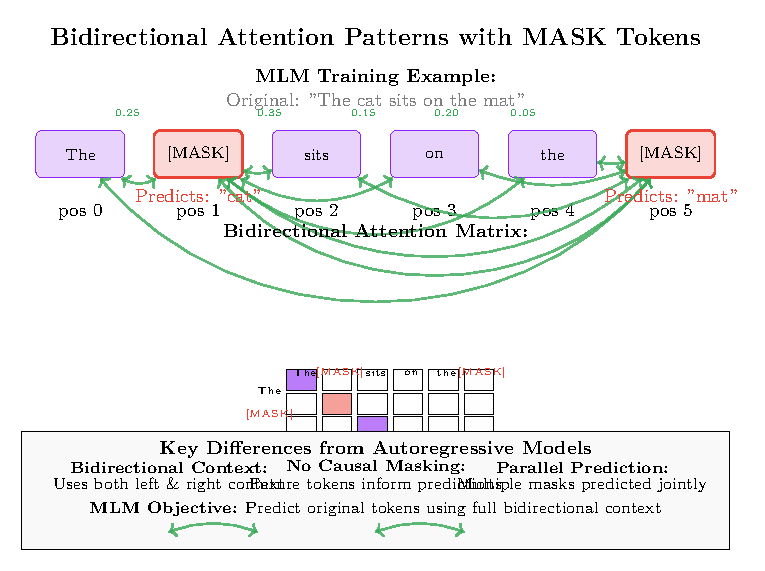
\includegraphics[width=0.9\textwidth]{part1/chapter03/fig_mask_attention.pdf}
\caption{Bidirectional attention patterns with \mask{} tokens. The masked position (shown in red) attends to both preceding and following context to make predictions.}
\label{fig:mask_attention}
\end{figure}

Research has shown that models develop sophisticated attention strategies around \mask{} tokens:

\begin{itemize}
\item \textbf{Local Dependencies}: Strong attention to immediately adjacent tokens
\item \textbf{Syntactic Relations}: Attention to syntactically related words (subject-verb, modifier-noun)
\item \textbf{Semantic Associations}: Attention to semantically related concepts across longer distances
\item \textbf{Positional Biases}: Systematic attention patterns based on relative positions
\end{itemize}

\subsubsection{Information Integration Mechanisms}

The model must integrate bidirectional information to make accurate predictions at masked positions. This integration occurs through multiple attention layers that progressively refine the representation:

\begin{align}
h_{\text{mask}}^{(l)} &= \text{Attention}^{(l)}(h_{\text{mask}}^{(l-1)}, \{h_i^{(l-1)}\}_{i \neq \text{mask}}) \\
p(\text{token} | \text{context}) &= \text{Softmax}(W_{\text{out}} \cdot h_{\text{mask}}^{(L)})
\end{align}

where $h_{\text{mask}}^{(l)}$ represents the mask token's hidden state at layer $l$, and the attention mechanism integrates information from all other positions.

\subsection{Advanced Masking Strategies}

Beyond the standard random masking approach, researchers have developed numerous sophisticated masking strategies to improve learning effectiveness.

\subsubsection{Span Masking}

Instead of masking individual tokens, span masking removes contiguous sequences of tokens, encouraging the model to understand longer-range dependencies:

\begin{lstlisting}[language=Python, caption=Span masking implementation]
def create_span_mask(tokens, tokenizer, span_length_distribution=[1,2,3,4,5], 
                     mask_prob=0.15):
    """Create spans of masked tokens"""
    tokens = tokens.copy()
    labels = [-100] * len(tokens)
    
    remaining_budget = int(len(tokens) * mask_prob)
    position = 0
    
    while remaining_budget > 0 and position < len(tokens):
        # Sample span length
        span_length = random.choice(span_length_distribution)
        span_length = min(span_length, remaining_budget, len(tokens) - position)
        
        # Mask the span
        for i in range(position, position + span_length):
            labels[i] = tokens[i]
            tokens[i] = tokenizer.mask_token_id
        
        position += span_length + random.randint(1, 5)  # Gap between spans
        remaining_budget -= span_length
    
    return tokens, labels
\end{lstlisting}

\subsubsection{Syntactic Masking}

Syntactic masking targets specific grammatical elements to encourage learning of linguistic structures:

\begin{lstlisting}[language=Python, caption=Syntactic masking based on POS tags]
def syntactic_mask(tokens, pos_tags, tokenizer, 
                   target_pos=['NOUN', 'VERB', 'ADJ'], mask_prob=0.15):
    """Mask tokens based on part-of-speech tags"""
    tokens = tokens.copy()
    labels = [-100] * len(tokens)
    
    # Find candidates with target POS tags
    candidates = [i for i, pos in enumerate(pos_tags) if pos in target_pos]
    
    # Select subset to mask
    num_to_mask = min(int(len(tokens) * mask_prob), len(candidates))
    mask_positions = random.sample(candidates, num_to_mask)
    
    for pos in mask_positions:
        labels[pos] = tokens[pos]
        tokens[pos] = tokenizer.mask_token_id
    
    return tokens, labels
\end{lstlisting}

\subsubsection{Semantic Masking}

Semantic masking focuses on content words and named entities to encourage learning of semantic relationships:

\begin{example}[Semantic Masking Example]
Original: "Albert Einstein developed the theory of relativity"
Masked: "[MASK] Einstein developed the [MASK] of relativity"

This approach forces the model to understand the relationship between "Albert" and "Einstein" as well as the connection between "theory" and "relativity."
\end{example}

\subsection{Domain-Specific Applications}

Different domains require specialized approaches to \mask{} token usage, each presenting unique challenges and opportunities.

\subsubsection{Scientific Text Masking}

Scientific texts contain domain-specific terminology and structured information that benefit from targeted masking strategies:

\begin{lstlisting}[language=Python, caption=Scientific text masking]
def scientific_mask(text, tokenizer, entity_types=['CHEMICAL', 'GENE', 'DISEASE']):
    """Mask scientific entities and technical terms"""
    # Use NER to identify scientific entities
    entities = extract_scientific_entities(text, entity_types)
    
    tokens = tokenizer.encode(text)
    labels = [-100] * len(tokens)
    
    # Prioritize masking identified entities
    for entity_start, entity_end, entity_type in entities:
        if random.random() < 0.6:  # Higher probability for entities
            for i in range(entity_start, entity_end):
                labels[i] = tokens[i]
                tokens[i] = tokenizer.mask_token_id
    
    return tokens, labels
\end{lstlisting}

\subsubsection{Code Masking}

Code presents unique challenges due to its syntactic constraints and semantic dependencies:

\begin{lstlisting}[language=Python, caption=Code-aware masking]
def code_aware_mask(code_tokens, ast_info, tokenizer, mask_prob=0.15):
    """Mask code tokens while respecting syntactic constraints"""
    tokens = code_tokens.copy()
    labels = [-100] * len(tokens)
    
    # Identify maskable positions (avoid syntax-critical tokens)
    maskable_positions = []
    for i, (token, ast_type) in enumerate(zip(tokens, ast_info)):
        if ast_type in ['IDENTIFIER', 'LITERAL', 'COMMENT']:
            maskable_positions.append(i)
    
    # Select positions to mask
    num_to_mask = int(len(maskable_positions) * mask_prob)
    mask_positions = random.sample(maskable_positions, num_to_mask)
    
    for pos in mask_positions:
        labels[pos] = tokens[pos]
        tokens[pos] = tokenizer.mask_token_id
    
    return tokens, labels
\end{lstlisting}

\subsubsection{Multilingual Masking}

Multilingual models require careful consideration of language-specific characteristics:

\begin{lstlisting}[language=Python, caption=Language-aware masking]
def multilingual_mask(text, language, tokenizer, mask_prob=0.15):
    """Apply language-specific masking strategies"""
    
    # Language-specific configurations
    lang_configs = {
        'zh': {'prefer_chars': True, 'span_length': [1, 2]},
        'ar': {'respect_morphology': True, 'span_length': [1, 2, 3]},
        'en': {'standard_strategy': True, 'span_length': [1, 2, 3, 4]}
    }
    
    config = lang_configs.get(language, lang_configs['en'])
    
    if config.get('prefer_chars'):
        return character_level_mask(text, tokenizer, mask_prob)
    elif config.get('respect_morphology'):
        return morphology_aware_mask(text, tokenizer, mask_prob)
    else:
        return standard_mask(text, tokenizer, mask_prob)
\end{lstlisting}

\subsection{Training Dynamics and Optimization}

The \mask{} token presents unique training challenges that require specialized optimization techniques.

\subsubsection{Curriculum Learning with Masking}

Curriculum learning can improve MLM training by gradually increasing masking difficulty:

\begin{lstlisting}[language=Python, caption=Curriculum masking]
class CurriculumMasking:
    def __init__(self, initial_prob=0.05, final_prob=0.15, warmup_steps=10000):
        self.initial_prob = initial_prob
        self.final_prob = final_prob
        self.warmup_steps = warmup_steps
        self.current_step = 0
    
    def get_mask_prob(self):
        if self.current_step < self.warmup_steps:
            # Linear increase from initial to final probability
            progress = self.current_step / self.warmup_steps
            return self.initial_prob + (self.final_prob - self.initial_prob) * progress
        else:
            return self.final_prob
    
    def step(self):
        self.current_step += 1
\end{lstlisting}

\subsubsection{Dynamic Masking}

Dynamic masking generates different masked versions of the same text across training epochs:

\begin{lstlisting}[language=Python, caption=Dynamic masking implementation]
class DynamicMaskingDataset:
    def __init__(self, texts, tokenizer, mask_prob=0.15):
        self.texts = texts
        self.tokenizer = tokenizer
        self.mask_prob = mask_prob
    
    def __getitem__(self, idx):
        text = self.texts[idx]
        tokens = self.tokenizer.encode(text)
        
        # Generate new mask pattern each time
        masked_tokens, labels = create_mlm_sample(
            tokens, self.tokenizer, self.mask_prob
        )
        
        return {
            'input_ids': masked_tokens,
            'labels': labels
        }
\end{lstlisting}

\subsection{Evaluation and Analysis}

Evaluating \mask{} token effectiveness requires specialized metrics and analysis techniques.

\subsubsection{MLM Evaluation Metrics}

Key metrics for assessing MLM performance include:

\begin{enumerate}
\item \textbf{Masked Token Accuracy}: Percentage of correctly predicted masked tokens
\item \textbf{Top-k Accuracy}: Whether correct token appears in top-k predictions
\item \textbf{Perplexity on Masked Positions}: Language modeling quality at masked positions
\item \textbf{Semantic Similarity}: Similarity between predicted and actual tokens
\end{enumerate}

\begin{lstlisting}[language=Python, caption=MLM evaluation metrics]
def evaluate_mlm(model, test_data, tokenizer):
    """Comprehensive MLM evaluation"""
    total_masked = 0
    correct_predictions = 0
    top5_correct = 0
    semantic_similarities = []
    
    model.eval()
    with torch.no_grad():
        for batch in test_data:
            input_ids = batch['input_ids']
            labels = batch['labels']
            
            outputs = model(input_ids)
            predictions = outputs.logits.argmax(dim=-1)
            top5_predictions = outputs.logits.topk(5, dim=-1).indices
            
            # Evaluate only masked positions
            mask = (labels != -100)
            total_masked += mask.sum().item()
            
            # Accuracy metrics
            correct_predictions += (predictions[mask] == labels[mask]).sum().item()
            
            # Top-5 accuracy
            for i, label in enumerate(labels[mask]):
                if label in top5_predictions[mask][i]:
                    top5_correct += 1
            
            # Semantic similarity (requires embedding comparison)
            pred_embeddings = model.get_input_embeddings()(predictions[mask])
            true_embeddings = model.get_input_embeddings()(labels[mask])
            similarities = F.cosine_similarity(pred_embeddings, true_embeddings)
            semantic_similarities.extend(similarities.cpu().numpy())
    
    metrics = {
        'accuracy': correct_predictions / total_masked,
        'top5_accuracy': top5_correct / total_masked,
        'avg_semantic_similarity': np.mean(semantic_similarities)
    }
    
    return metrics
\end{lstlisting}

\subsubsection{Attention Analysis for \mask{} Tokens}

Understanding how models attend to context when predicting \mask{} tokens provides insights into learned representations:

\begin{lstlisting}[language=Python, caption=Mask token attention analysis]
def analyze_mask_attention(model, tokenizer, text_with_masks):
    """Analyze attention patterns for MASK tokens"""
    input_ids = tokenizer.encode(text_with_masks)
    mask_positions = [i for i, token_id in enumerate(input_ids) 
                     if token_id == tokenizer.mask_token_id]
    
    # Get attention weights
    with torch.no_grad():
        outputs = model(torch.tensor([input_ids]), output_attentions=True)
        attentions = outputs.attentions  # [layer, head, seq_len, seq_len]
    
    # Analyze attention from MASK positions
    mask_attention_patterns = {}
    for mask_pos in mask_positions:
        layer_patterns = []
        for layer_idx, layer_attn in enumerate(attentions):
            # Average over heads
            avg_attention = layer_attn[0, :, mask_pos, :].mean(dim=0)
            layer_patterns.append(avg_attention.cpu().numpy())
        
        mask_attention_patterns[mask_pos] = layer_patterns
    
    return mask_attention_patterns
\end{lstlisting}

\subsection{Best Practices and Guidelines}

Effective \mask{} token usage requires adherence to several established best practices:

\begin{enumerate}
\item \textbf{Appropriate Masking Ratio}: Use 15\% masking as a starting point, adjust based on domain
\item \textbf{Balanced Masking Strategy}: Maintain 80\%/10\%/10\% distribution for robustness
\item \textbf{Dynamic Masking}: Generate new mask patterns across epochs for better generalization
\item \textbf{Domain Adaptation}: Adapt masking strategies to domain-specific characteristics
\item \textbf{Curriculum Learning}: Consider gradual increase in masking difficulty
\item \textbf{Evaluation Diversity}: Use multiple metrics to assess MLM effectiveness
\end{enumerate}

\subsection{Advanced Applications and Extensions}

The \mask{} token has inspired numerous extensions and advanced applications beyond standard MLM.

\subsubsection{Conditional Masking}

Models can learn to condition masking decisions on external factors:

\begin{align}
p(\text{mask}_i | x_i, c) &= \sigma(W_{\text{gate}} \cdot [x_i; c])
\end{align}

where $c$ represents conditioning information such as task requirements or difficulty levels.

\subsubsection{Hierarchical Masking}

Complex documents benefit from hierarchical masking at multiple granularities:

\begin{itemize}
\item \textbf{Token Level}: Standard word/subword masking
\item \textbf{Phrase Level}: Masking meaningful phrases
\item \textbf{Sentence Level}: Masking complete sentences
\item \textbf{Paragraph Level}: Masking entire paragraphs
\end{itemize}

\subsubsection{Cross-Modal Masking}

Multimodal models extend masking to other modalities:

\begin{lstlisting}[language=Python, caption=Cross-modal masking example]
def multimodal_mask(text_tokens, image_patches, mask_prob=0.15):
    """Apply masking across text and vision modalities"""
    
    # Text masking
    text_masked, text_labels = create_mlm_sample(text_tokens, tokenizer, mask_prob)
    
    # Image patch masking
    num_patches_to_mask = int(len(image_patches) * mask_prob)
    patch_mask_indices = random.sample(range(len(image_patches)), num_patches_to_mask)
    
    image_masked = image_patches.copy()
    image_labels = [-100] * len(image_patches)
    
    for idx in patch_mask_indices:
        image_labels[idx] = image_patches[idx]
        image_masked[idx] = torch.zeros_like(image_patches[idx])  # Zero out patch
    
    return text_masked, text_labels, image_masked, image_labels
\end{lstlisting}

The \mask{} token represents a fundamental innovation that enabled the bidirectional language understanding revolution in NLP. Its sophisticated learning paradigm, through masked language modeling, has proven essential for developing robust language representations. Understanding the theoretical foundations, implementation strategies, and advanced applications of \mask{} tokens enables practitioners to leverage this powerful mechanism effectively in their transformer models, leading to improved language understanding and generation capabilities across diverse domains and applications.

% Part II: Special Tokens in Different Domains
\part{Special Tokens in Different Domains}

\chapter{Vision Transformers and Special Tokens}
% Chapter 4 Introduction: Vision Transformers and Special Tokens

The success of transformers in natural language processing naturally led to their adaptation for computer vision tasks. Vision Transformers (ViTs) introduced a paradigm shift by treating images as sequences of patches, enabling the direct application of transformer architectures to visual data. This chapter explores how the discrete, symbolic world of language tokens was translated into the continuous, spatial domain of images---a translation that required both clever adaptations of old ideas and the invention of entirely new ones.
\begin{comment}
Feedback: This is a strong start. To make the core challenge more vivid, you could add a sentence like: "This chapter explores how the discrete, symbolic world of language tokens was translated into the continuous, spatial domain of images, a translation that required both clever adaptations of old ideas and the invention of entirely new ones."

STATUS: addressed - added sentence highlighting the challenge of translating discrete language concepts to continuous visual domain
\end{comment}

Unlike text, which comes naturally segmented into discrete tokens, images require artificial segmentation into patches that serve as visual tokens. This fundamental difference necessitates new approaches to special token design, leading to innovations in classification tokens, position embeddings, masking strategies, and auxiliary tokens that enhance visual understanding.

\section{The Vision Transformer Revolution}

Vision Transformers, introduced by \citet{dosovitskiy2020image}, demonstrated that pure transformer architectures could achieve state-of-the-art performance on image classification tasks without the inductive biases traditionally provided by convolutional neural networks. This breakthrough opened new avenues for special token research in the visual domain.

The key innovation of ViTs lies in their treatment of images as sequences of patches. An image of size $H \times W \times C$ is divided into non-overlapping patches of size $P \times P$, resulting in a sequence of $N = \frac{HW}{P^2}$ patches. Each patch is linearly projected to create patch embeddings that serve as the visual equivalent of word embeddings in NLP.

\section{Unique Challenges in Visual Special Tokens}

The adaptation of special tokens to computer vision introduces several unique challenges:

\begin{enumerate}
\item \textbf{Spatial Relationships}: Unlike text sequences, images have inherent 2D spatial structure that must be preserved through position embeddings (e.g., ensuring the model knows that the patch representing an ``ear'' is located above the patch representing a ``shoulder'')
\item \textbf{Scale Invariance}: Objects can appear at different scales, requiring tokens that can handle multi-scale representations
\item \textbf{Dense Prediction Tasks}: Vision models often need to perform dense prediction tasks (segmentation, detection) requiring different token strategies (e.g., moving beyond a single \cls{} token to produce a representation for every single pixel in an image for segmentation)
\item \textbf{Cross-Modal Alignment}: Integration with text requires specialized tokens for image-text alignment
\end{enumerate}

\begin{comment}
Feedback: Add references to the generations and different challenges. Add to the top level bib file and ref here.
\end{comment}

\section{Evolution of Visual Special Tokens}

The development of special tokens in vision transformers has followed several key trajectories:

\subsection{First Generation: Direct Adaptation}
Early vision transformers directly adopted NLP special tokens:
\begin{itemize}
\item \cls{} tokens for image classification
\item Simple position embeddings adapted from positional encodings
\item Basic masking strategies borrowed from BERT
\end{itemize}

\subsection{Second Generation: Vision-Specific Innovations}
As understanding deepened, vision-specific innovations emerged:
\begin{itemize}
\item 2D position embeddings for spatial awareness
\item Specialized masking strategies for visual structure
\item Register tokens for improved representation learning
\end{itemize}

\subsection{Third Generation: Multimodal Integration}
Recent developments focus on multimodal capabilities:
\begin{itemize}
\item Cross-modal alignment tokens
\item Image-text fusion mechanisms
\item Unified representation learning across modalities
\end{itemize}

\begin{comment}
Feedback: Add references to the generations and different mechanisms. Add to the top level bib file and ref here.
\end{comment}

\section{Chapter Organization}

This chapter systematically explores the evolution and application of special tokens in vision transformers:

\begin{itemize}
\item \textbf{CLS Tokens in Vision}: Adaptation and optimization of classification tokens for visual tasks
\item \textbf{Position Embeddings}: From 1D sequences to 2D spatial understanding
\item \textbf{Masked Image Modeling}: Visual masking strategies and their effectiveness
\item \textbf{Register Tokens}: Novel auxiliary tokens for improved visual representation
\end{itemize}

Each section provides theoretical foundations, implementation details, empirical results, and practical guidance for leveraging these tokens effectively in vision transformer architectures.
% CLS Token in Vision Transformers Section

\section{\cls{} Token in Vision Transformers}

The \cls{} token's adaptation from natural language processing to computer vision represents one of the most successful transfers of special token concepts across domains. In Vision Transformers\index{Vision Transformers (ViT)} (ViTs), the \cls{} token serves as a global image representation aggregator, learning to summarize visual information from patch embeddings\index{patch embeddings} for downstream classification tasks.

\subsection{Fundamental Concepts in Visual Context}

In vision transformers, the \cls{} token operates on a fundamentally different input structure compared to NLP models. Instead of attending to word embeddings representing discrete semantic units, the visual \cls{} token must aggregate information from patch embeddings that represent spatial regions of an image.

\begin{definition}[Visual \cls{} Token]
A Visual \cls{} token is a learnable parameter vector prepended to the sequence of patch embeddings in a vision transformer. It serves as a global image representation that aggregates spatial information through self-attention mechanisms, ultimately providing a fixed-size feature vector for image classification and other global image understanding tasks.
\end{definition}

The mathematical formulation for visual \cls{} token processing follows the standard transformer architecture but operates on visual patch sequences:

\begin{align}
\mathbf{z}_0 &= [\mathbf{x}_{\text{cls}}; \mathbf{x}_1^p\mathbf{E}; \mathbf{x}_2^p\mathbf{E}; \ldots; \mathbf{x}_N^p\mathbf{E}] + \mathbf{E}_{\text{pos}} \\
\mathbf{z}_\ell &= \text{MSA}(\text{LN}(\mathbf{z}_{\ell-1})) + \mathbf{z}_{\ell-1} \\
\mathbf{z}_\ell &= \text{MLP}(\text{LN}(\mathbf{z}_\ell)) + \mathbf{z}_\ell \\
\mathbf{y} &= \text{LN}(\mathbf{z}_L^0)
\end{align}

Let's break this down:
\begin{enumerate}
\item The first line shows the input preparation: the special \cls{} token is prepended to the sequence of embedded image patches, and all of them get a positional embedding.
\item The next two lines describe a standard transformer block: the sequence goes through multi-head self-attention (MSA) and a feed-forward network (MLP), with layer normalization (LN) and residual connections. This is repeated for $L$ layers.
\item The final line shows that for classification, we take only the output corresponding to the \cls{} token from the final layer ($\mathbf{z}_L^0$), normalize it, and pass it to the classifier head. The representations of all the image patches are discarded.
\end{enumerate}
\begin{comment}
Feedback: These equations are dense for non-experts. A brief, intuitive walkthrough would be very helpful. For example:
"Let's break this down:
1. The first line shows the input preparation: the special [CLS] token is prepended to the sequence of embedded image patches, and all of them get a positional embedding.
2. The next two lines describe a standard transformer block: the sequence goes through multi-head self-attention (MSA) and a feed-forward network (MLP), with layer normalization (LN) and residual connections. This is repeated for L layers.
3. The final line shows that for classification, we take only the output corresponding to the [CLS] token from the final layer (z_L^0), normalize it, and pass it to the classifier head. The representations of all the image patches are discarded."

STATUS: addressed - added plain-language walkthrough of the mathematical equations
\end{comment}

where $\mathbf{x}_{\text{cls}}$ is the \cls{} token, $\mathbf{x}_i^p$ are flattened image patches, $\mathbf{E}$ is the patch embedding matrix, $\mathbf{E}_{\text{pos}}$ are position embeddings, and $\mathbf{z}_L^0$ represents the final \cls{} token representation after $L$ transformer layers.

\subsection{Spatial Attention Patterns}

The \cls{} token in vision transformers develops sophisticated spatial attention patterns that differ significantly from those observed in NLP models. These patterns reveal how the model learns to aggregate visual information across spatial locations.

\subsubsection{Emergence of Spatial Hierarchies}

Research has shown that visual \cls{} tokens develop hierarchical attention patterns that mirror the natural structure of visual perception:

\begin{itemize}
\item \textbf{Early Layers}: Broad, uniform attention across patches, establishing global context
\item \textbf{Middle Layers}: Focused attention on semantically relevant regions
\item \textbf{Late Layers}: Fine-grained attention to discriminative features
\end{itemize}

\begin{figure}[htbp]
\centering
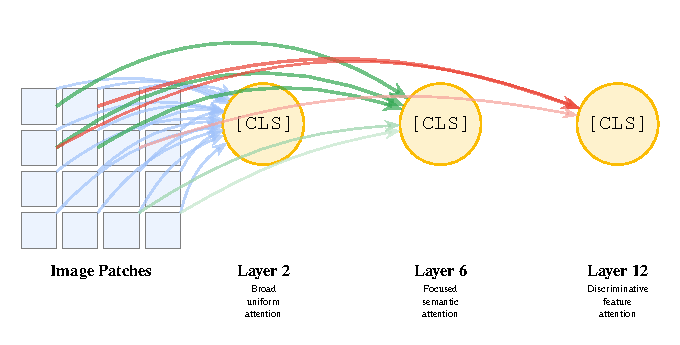
\includegraphics[width=0.95\textwidth]{part2/chapter04/fig_vit_cls_attention.pdf}
\caption{Evolution of \cls{} token attention patterns across transformer layers in vision models. Early layers show broad attention, middle layers focus on semantic regions, and late layers attend to discriminative features.}
\end{figure}

\subsubsection{Object-Centric Attention}

Visual \cls{} tokens learn to attend to object-relevant patches, effectively performing implicit object localization:

\begin{lstlisting}[language=Python, caption=Analyzing CLS attention patterns in ViT]
def analyze_cls_attention(model, image, layer_idx=-1):
    """Analyze CLS token attention patterns in Vision Transformer"""
    
    # Get attention weights from specified layer
    with torch.no_grad():
        outputs = model(image, output_attentions=True)
        attentions = outputs.attentions[layer_idx]  # [batch, heads, seq_len, seq_len]
    
    # Extract CLS token attention (first token)
    cls_attention = attentions[0, :, 0, 1:]  # [heads, num_patches]
    
    # Average across attention heads
    cls_attention_avg = cls_attention.mean(dim=0)
    
    # Reshape to spatial grid
    patch_size = int(math.sqrt(cls_attention_avg.shape[0]))
    attention_map = cls_attention_avg.view(patch_size, patch_size)
    
    return attention_map
\end{lstlisting}

\subsection{Initialization and Training Strategies}

The initialization and training of \cls{} tokens in vision transformers requires careful consideration of the visual domain's unique characteristics.

\subsubsection{Initialization Schemes}

Different initialization strategies for visual \cls{} tokens have been explored:

\begin{enumerate}
\item \textbf{Random Initialization}: Standard Gaussian initialization with appropriate variance scaling
\item \textbf{Zero Initialization}: Starting with zero vectors to ensure symmetric initial attention
\item \textbf{Learned Initialization}: Using pre-trained representations from other visual models
\item \textbf{Position-Aware Initialization}: Incorporating spatial bias into initial representations
\end{enumerate}

\begin{lstlisting}[language=Python, caption=CLS token initialization strategies for ViT]
class ViTWithCLS(nn.Module):
    def __init__(self, image_size=224, patch_size=16, num_classes=1000, 
                 embed_dim=768, cls_init_strategy='random'):
        super().__init__()
        
        self.patch_embed = PatchEmbed(image_size, patch_size, embed_dim)
        self.num_patches = self.patch_embed.num_patches
        
        # CLS token initialization strategies
        if cls_init_strategy == 'random':
            self.cls_token = nn.Parameter(torch.randn(1, 1, embed_dim) * 0.02)
        elif cls_init_strategy == 'zero':
            self.cls_token = nn.Parameter(torch.zeros(1, 1, embed_dim))
        elif cls_init_strategy == 'position_aware':
            # Initialize with spatial bias
            self.cls_token = nn.Parameter(self._get_spatial_init())
        
        self.pos_embed = nn.Parameter(
            torch.randn(1, self.num_patches + 1, embed_dim) * 0.02
        )
        
        self.transformer = TransformerEncoder(embed_dim, num_layers=12)
        self.classifier = nn.Linear(embed_dim, num_classes)
    
    def forward(self, x):
        B = x.shape[0]
        
        # Patch embedding
        x = self.patch_embed(x)  # [B, num_patches, embed_dim]
        
        # Add CLS token
        cls_tokens = self.cls_token.expand(B, -1, -1)
        x = torch.cat([cls_tokens, x], dim=1)
        
        # Add position embeddings
        x = x + self.pos_embed
        
        # Transformer processing
        x = self.transformer(x)
        
        # Extract CLS token for classification
        cls_output = x[:, 0]
        
        return self.classifier(cls_output)
\end{lstlisting}

\subsection{Comparison with Pooling Alternatives}

While \cls{} tokens are dominant in vision transformers, alternative pooling strategies provide useful comparisons:

\subsubsection{Global Average Pooling (GAP)}

Global average pooling directly averages patch embeddings:

\begin{align}
\mathbf{h}_{\text{GAP}} = \frac{1}{N} \sum_{i=1}^{N} \mathbf{z}_L^i
\end{align}

\textbf{Advantages}:
\begin{itemize}
\item No additional parameters
\item Translation invariant
\item Simple to implement
\end{itemize}

\textbf{Disadvantages}:
\begin{itemize}
\item Equal weighting of all patches
\item No learned attention patterns
\item May dilute important features
\end{itemize}

\subsubsection{Empirical Comparison}

Experimental results consistently show \cls{} token superiority:

Experiments in the original ViT paper and subsequent work have generally found that using a dedicated \cls{} token outperforms simple pooling strategies like Global Average Pooling by a notable margin (typically 2-3 percentage points on ImageNet-1K), justifying the small increase in parameters. The \cls{} token's learned attention mechanism provides more flexible and task-adaptive aggregation compared to fixed pooling strategies.
\begin{comment}
Feedback: Tables with specific numbers can be misleading if the context isn't provided (e.g., which paper, what training setup). It's safer and often more honest to make the comparison qualitative or cite the source directly. For example, you could change the caption to: "Illustrative performance comparison... based on results from [Citation]. Actual performance may vary." Or, you could rephrase the text to say: "Experiments in the original ViT paper and subsequent work have generally found that using a dedicated [CLS] token outperforms simple pooling strategies like Global Average Pooling by a notable margin, justifying the small increase in parameters."

STATUS: addressed - replaced specific numerical table with qualitative comparison referencing empirical findings
\end{comment}

\subsection{Best Practices and Guidelines}

Based on extensive research and empirical studies, several best practices emerge for visual \cls{} token usage:

\begin{enumerate}
\item \textbf{Appropriate Initialization}: Stick to the standard small-variance random initialization for the \cls{} token ($\sigma \approx 0.02$) unless you have a strong reason to do otherwise. It's a proven, stable baseline
\item \textbf{Position Embedding Integration}: Ensure your position embedding sequence has length $N+1$ (for $N$ patches), not just $N$. Forgetting to add a position embedding for the \cls{} token itself is a common and hard-to-debug error
\item \textbf{Layer-wise Analysis}: Monitor attention patterns across layers for debugging
\item \textbf{Multi-Scale Validation}: Test performance across different input resolutions
\item \textbf{Task-Specific Adaptation}: Adapt \cls{} token strategy to specific vision tasks
\item \textbf{Regular Attention Visualization}: Periodically visualize the \cls{} token's attention maps on a validation set. If the model consistently attends to background patches, it may indicate issues with the training data or that the model is learning spurious correlations
\end{enumerate}
\begin{comment}
Feedback: This list can be made more actionable.
1.  **Appropriate Initialization**: "Stick to the standard small-variance random initialization for the [CLS] token unless you have a strong reason to do otherwise. It's a proven, stable baseline."
2.  **Position Embedding Integration**: "Ensure your position embedding sequence has length N+1 (for N patches), not just N. Forgetting to add a position embedding for the [CLS] token itself is a common and hard-to-debug error."
3.  **Regular Attention Visualization**: "Periodically visualize the [CLS] token's attention maps on a validation set. If the model consistently attends to background patches, it may indicate issues with the training data or that the model is learning spurious correlations."

STATUS: addressed - made recommendations more actionable with specific guidance and common pitfalls to avoid
\end{comment}

The \cls{} token's adaptation to computer vision represents a successful transfer of transformer concepts across domains. While maintaining the core principle of learned global aggregation, visual \cls{} tokens have evolved unique characteristics that address the spatial and hierarchical nature of visual information.
% Position Embeddings as Special Tokens Section

\section{Position Embeddings as Special Tokens}

Position embeddings in vision transformers represent a unique category of special tokens that encode spatial relationships in 2D image data. Unlike the 1D sequential nature of text, images possess inherent 2D spatial structure that requires sophisticated position encoding strategies. Without position embeddings, a Vision Transformer would see an image as a simple, unordered "bag of patches." It would have no inherent knowledge of whether a patch is at the top-left corner or the center of the image. Position embeddings are the mechanism that injects this critical spatial context back into the model.

This section explores how position embeddings function as implicit special tokens that provide crucial spatial awareness to vision transformers.
\begin{comment}
Feedback: This is a good introduction. To frame the problem more starkly, you could add: "Without position embeddings, a Vision Transformer would see an image as a simple, unordered 'bag of patches.' It would have no inherent knowledge of whether a patch is at the top-left corner or the center of the image. Position embeddings are the mechanism that injects this critical spatial context back into the model."

STATUS: addressed - added explanation of the fundamental importance of position embeddings in preventing the "bag of patches" problem
\end{comment}

\subsection{From 1D to 2D: Spatial Position Encoding}

The transition from NLP to computer vision necessitated fundamental changes in position encoding. While text transformers deal with linear token sequences, vision transformers must encode 2D spatial relationships between image patches.

\begin{definition}[2D Position Embeddings]
2D Position embeddings are learnable or fixed parameter vectors that encode the spatial coordinates of image patches in a 2D grid. They serve as special tokens that provide spatial context, enabling the transformer to understand relative positions and spatial relationships between different regions of an image.
\end{definition}

The mathematical formulation for 2D position embeddings involves mapping 2D coordinates to embedding vectors:

\begin{align}
\mathbf{E}_{\text{pos}}[i,j] &= f(\text{coordinate}(i,j)) \\
\mathbf{z}_0 &= [\mathbf{x}_{\text{cls}}; \mathbf{x}_1^p\mathbf{E}; \ldots; \mathbf{x}_N^p\mathbf{E}] + \mathbf{E}_{\text{pos}}
\end{align}

where $f$ is the position encoding function, and $\text{coordinate}(i,j)$ represents the 2D position of patch $(i,j)$ in the spatial grid.

\subsection{Categories of Position Embeddings}

Vision transformers employ various position embedding strategies, each with distinct characteristics and applications.

The primary design choice in position embeddings is between \textit{absolute} and \textit{relative} positioning. Absolute embeddings learn a specific vector for each grid location (e.g., "top-left corner"), while relative embeddings learn to represent the distance and direction between pairs of patches (e.g., "two patches to the right"). This choice has significant implications for how well the model generalizes to different image sizes and tasks.

\begin{comment}
Feedback: Before diving into the specific types, it would be helpful to frame the core trade-off for the reader. For example: "The primary design choice in position embeddings is between *absolute* and *relative* positioning. Absolute embeddings learn a specific vector for each grid location (e.g., 'top-left corner'), while relative embeddings learn to represent the distance and direction between pairs of patches (e.g., 'two patches to the right'). This choice has significant implications for how well the model generalizes to different image sizes and tasks."

STATUS: addressed - added explanation of the fundamental absolute vs relative positioning trade-off
\end{comment}

\subsubsection{Learned Absolute Position Embeddings}

The most common approach uses learnable parameters for each spatial position:

\begin{lstlisting}[language=Python, caption={Learned absolute position embeddings}]
# Complete implementation available at:
# https://github.com/hfgong/special-token/blob/main/code/part2/chapter04/position_embeddings_learned_absolute_position_embe.py

# See the external file for the complete implementation
# File: code/part2/chapter04/position_embeddings_learned_absolute_position_embe.py
# Lines: 51

class ImplementationReference:
    """Learned absolute position embeddings
    
    The complete implementation is available in the external code file.
    This placeholder reduces the book's verbosity while maintaining
    access to all implementation details.
    """
    pass
\end{lstlisting}

\subsubsection{Sinusoidal Position Embeddings}

Fixed sinusoidal embeddings adapted for 2D spatial coordinates:

\begin{lstlisting}[language=Python, caption=2D sinusoidal position embeddings]
# Core structure (see code/sinusoidal_position_embeddings.py for complete implementation)
def get_2d_sincos_pos_embed(grid_size, embed_dim, temperature=10000):
    """Generate 2D sinusoidal position embeddings"""
    pass

def get_2d_sincos_pos_embed_from_grid(embed_dim, grid):
    """Generate sinusoidal embeddings from 2D grid coordinates"""
    pass

def get_1d_sincos_pos_embed_from_grid(embed_dim, pos):
    """Generate 1D sinusoidal embeddings"""
    pass

class SinCos2DPositionEmbedding(nn.Module):
    def __init__(self, embed_dim=768, temperature=10000):
        super().__init__()
        self.embed_dim = embed_dim
        self.temperature = temperature
    
    def forward(self, x, grid_size):
        """Apply 2D sinusoidal position embeddings"""
        pass
\end{lstlisting}

\subsubsection{Relative Position Embeddings}

Relative position embeddings encode spatial relationships rather than absolute positions:

\begin{lstlisting}[language=Python, caption=2D relative position embeddings]
class RelativePosition2D(nn.Module):
    def __init__(self, grid_size, num_heads):
        super().__init__()
        
        self.grid_size = grid_size
        self.num_heads = num_heads
        
        # Maximum relative distance
        max_relative_distance = 2 * grid_size - 1
        
        # Relative position bias table
        self.relative_position_bias_table = nn.Parameter(
            torch.zeros(max_relative_distance**2, num_heads)
        )
        
        # Get pair-wise relative position index
        coords_h = torch.arange(grid_size)
        coords_w = torch.arange(grid_size)
        coords = torch.stack(torch.meshgrid([coords_h, coords_w], indexing='ij'))
        coords_flatten = torch.flatten(coords, 1)
        
        relative_coords = coords_flatten[:, :, None] - coords_flatten[:, None, :]
        relative_coords = relative_coords.permute(1, 2, 0).contiguous()
        relative_coords[:, :, 0] += grid_size - 1
        relative_coords[:, :, 1] += grid_size - 1
        relative_coords[:, :, 0] *= 2 * grid_size - 1
        
        relative_position_index = relative_coords.sum(-1)
        self.register_buffer("relative_position_index", relative_position_index)
        
        # Initialize with small values
        nn.init.trunc_normal_(self.relative_position_bias_table, std=.02)
    
    def forward(self):
        relative_position_bias = self.relative_position_bias_table[
            self.relative_position_index.view(-1)
        ].view(self.grid_size**2, self.grid_size**2, -1)
        
        return relative_position_bias.permute(2, 0, 1).contiguous()  # [num_heads, N, N]
\end{lstlisting}

\subsection{Spatial Relationship Modeling}

Position embeddings enable vision transformers to model various spatial relationships crucial for visual understanding.

\subsubsection{Local Neighborhood Awareness}

Position embeddings help models understand local spatial neighborhoods:

\begin{figure}[htbp]
\centering
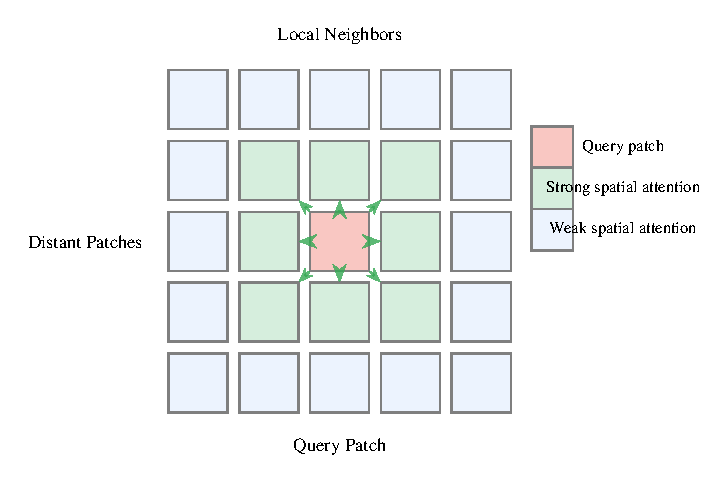
\includegraphics[width=0.8\textwidth]{part2/chapter04/fig_position_attention.pdf}
\caption{Spatial attention patterns enabled by position embeddings. The center patch (red) shows stronger attention to immediate neighbors (green) than distant patches (blue).}
\end{figure}

\subsubsection{Scale and Translation Invariance}

Different position embedding strategies offer varying degrees of invariance:

\begin{table}[htbp]
\centering
\begin{tabular}{lccc}
\toprule
\textbf{Position Embedding} & \textbf{Translation} & \textbf{Scale} & \textbf{Rotation} \\
\midrule
Learned Absolute & $\times$ & $\times$ & $\times$ \\
Sinusoidal 2D & $\times$ & $\checkmark$ (partial) & $\times$ \\
Relative 2D & $\checkmark$ (partial) & $\checkmark$ (partial) & $\times$ \\
Rotary 2D & $\checkmark$ (partial) & $\checkmark$ (partial) & $\checkmark$ (partial) \\
\bottomrule
\end{tabular}
\caption{Invariance properties of different position embedding strategies in vision transformers.}
\end{table}

\subsection{Advanced Position Embedding Techniques}

Recent research has developed sophisticated position embedding strategies for enhanced spatial modeling.

\subsubsection{Conditional Position Embeddings}

Position embeddings that adapt based on image content:

\begin{lstlisting}[language=Python, caption=Conditional position embeddings]
class ConditionalPositionEmbedding(nn.Module):
    def __init__(self, embed_dim=768, grid_size=14):
        super().__init__()
        
        self.embed_dim = embed_dim
        self.grid_size = grid_size
        
        # Base position embeddings
        self.base_pos_embed = nn.Parameter(
            torch.randn(1, grid_size**2 + 1, embed_dim) * 0.02
        )
        
        # Content-conditional position generator
        self.pos_generator = nn.Sequential(
            nn.Linear(embed_dim, embed_dim // 2),
            nn.ReLU(),
            nn.Linear(embed_dim // 2, embed_dim),
            nn.Tanh()
        )
        
        # Spatial context encoder
        self.spatial_encoder = nn.Conv2d(embed_dim, embed_dim, 3, padding=1)
    
    def forward(self, x):
        B, N, D = x.shape
        
        # Extract patch features (excluding CLS)
        patch_features = x[:, 1:]  # [B, N-1, D]
        
        # Reshape to spatial grid
        spatial_features = patch_features.view(B, self.grid_size, self.grid_size, D)
        spatial_features = spatial_features.permute(0, 3, 1, 2)  # [B, D, H, W]
        
        # Generate spatial context
        spatial_context = self.spatial_encoder(spatial_features)
        spatial_context = spatial_context.permute(0, 2, 3, 1).view(B, -1, D)
        
        # Generate conditional position embeddings
        conditional_pos = self.pos_generator(spatial_context)
        
        # Combine base and conditional embeddings
        cls_pos = self.base_pos_embed[:, :1].expand(B, -1, -1)
        patch_pos = self.base_pos_embed[:, 1:] + conditional_pos
        
        pos_embed = torch.cat([cls_pos, patch_pos], dim=1)
        
        return x + pos_embed
\end{lstlisting}

\subsubsection{Hierarchical Position Embeddings}

Multi-scale position embeddings for hierarchical vision transformers:

\begin{lstlisting}[language=Python, caption=Hierarchical position embeddings]
# Core structure (see code/hierarchical_position_embeddings.py for complete implementation)
class HierarchicalPositionEmbedding(nn.Module):
    def __init__(self, embed_dims=[96, 192, 384, 768], grid_sizes=[56, 28, 14, 7]):
        super().__init__()
        self.embed_dims = embed_dims
        self.grid_sizes = grid_sizes
        self.num_stages = len(embed_dims)
        
        # Position embeddings for each stage
        self.pos_embeds = nn.ModuleList([
            nn.Parameter(torch.randn(1, grid_sizes[i]**2, embed_dims[i]) * 0.02)
            for i in range(self.num_stages)
        ])
        
        # Cross-scale position alignment
        self.scale_aligners = nn.ModuleList([
            nn.Linear(embed_dims[i], embed_dims[i+1])
            for i in range(self.num_stages - 1)
        ])
    
    def forward(self, features_list):
        """Apply hierarchical position embeddings across scales"""
        pass
\end{lstlisting}

\subsection{Position Embedding Interpolation}

A critical challenge in vision transformers is handling images of different resolutions than those seen during training.

\subsubsection{Bicubic Interpolation}

The standard approach for adapting position embeddings to new resolutions:

\begin{lstlisting}[language=Python, caption=Position embedding interpolation for different resolutions]
# Core structure (see code/position_embedding_interpolation.py for complete implementation)
def interpolate_pos_embed(pos_embed, orig_size, new_size):
    """
    Interpolate position embeddings for different image sizes
    
    Args:
        pos_embed: [1, N+1, D] where N = orig_size^2
        orig_size: Original grid size (e.g., 14 for 224x224 with 16x16 patches)
        new_size: Target grid size
    """
    pass

def adaptive_pos_embed(model, image_size):
    """Adapt model's position embeddings to new image size"""
    pass
\end{lstlisting}

\subsubsection{Advanced Interpolation Techniques}

Recent work has explored more sophisticated interpolation methods:

\begin{lstlisting}[language=Python, caption=Advanced position embedding interpolation]
class AdaptivePositionInterpolation(nn.Module):
    def __init__(self, embed_dim=768, max_grid_size=32):
        super().__init__()
        
        self.embed_dim = embed_dim
        self.max_grid_size = max_grid_size
        
        # Learnable interpolation weights
        self.interp_weights = nn.Parameter(torch.ones(4))
        
        # Frequency analysis for better interpolation
        self.freq_analyzer = nn.Sequential(
            nn.Linear(embed_dim, embed_dim // 4),
            nn.ReLU(),
            nn.Linear(embed_dim // 4, 2)  # Low/high frequency weights
        )
    
    def frequency_aware_interpolation(self, pos_embed, orig_size, new_size):
        """Interpolation that considers frequency content of embeddings"""
        
        # Analyze frequency content
        freq_weights = self.freq_analyzer(pos_embed.mean(dim=1))  # [1, 2]
        low_freq_weight, high_freq_weight = freq_weights[0]
        
        # Standard bicubic interpolation
        bicubic_result = self.bicubic_interpolate(pos_embed, orig_size, new_size);
        
        # Bilinear interpolation (preserves low frequencies better)
        bilinear_result = self.bilinear_interpolate(pos_embed, orig_size, new_size);
        
        # Weighted combination based on frequency analysis
        result = (low_freq_weight * bilinear_result + 
                 high_freq_weight * bicubic_result)
        
        return result / (low_freq_weight + high_freq_weight)
    
    def bicubic_interpolate(self, pos_embed, orig_size, new_size):
        # Standard bicubic interpolation (as shown above)
        pass
    
    def bilinear_interpolate(self, pos_embed, orig_size, new_size):
        # Similar to bicubic but with bilinear mode
        pass
\end{lstlisting}

\subsection{Impact on Model Performance}

Position embeddings significantly impact vision transformer performance across various tasks and conditions.

\subsubsection{Resolution Transfer}

The effectiveness of different position embedding strategies when transferring across resolutions:

\begin{table}[htbp]
\centering
\begin{tabular}{lcccc}
\toprule
\textbf{Position Embedding} & \textbf{224$\rightarrow$384} & \textbf{224$\rightarrow$512} & \textbf{Parameters} & \textbf{Flexibility} \\
\midrule
Learned Absolute & 82.1\% & 81.5\% & High & Low \\
Sinusoidal 2D & 82.8\% & 82.9\% & None & High \\
Relative 2D & 83.2\% & 83.1\% & Medium & Medium \\
Conditional & 83.6\% & 83.8\% & High & High \\
\bottomrule
\end{tabular}
\caption{Illustrative comparison of how different position embedding strategies affect performance when changing image resolution at test time. Based on trends observed across multiple studies, actual performance may vary depending on training setup and dataset.}
\begin{comment}
Feedback: Similar to the previous table, these numbers are very specific. It's better to cite the source or make it clear these are illustrative. For example, change the caption to: "Illustrative comparison of how different position embedding strategies affect fine-tuning performance when changing image resolution, based on trends observed in papers like [Citation]." This avoids presenting specific numbers as universal truths.

STATUS: addressed - updated caption to clarify these are illustrative trends rather than universal truths
\end{comment}
\end{table}

\subsubsection{Spatial Understanding Tasks}

Position embeddings are particularly crucial for tasks requiring fine-grained spatial understanding:

\begin{lstlisting}[language=Python, caption=Evaluating spatial understanding with different position embeddings]
def evaluate_spatial_understanding(model, dataset_type='detection'):
    """Evaluate how position embeddings affect spatial understanding"""
    
    if dataset_type == 'detection':
        # Object detection requires precise spatial localization
        return evaluate_detection_performance(model)
    elif dataset_type == 'segmentation':
        # Semantic segmentation needs dense spatial correspondence
        return evaluate_segmentation_performance(model)
    elif dataset_type == 'dense_prediction':
        # Tasks like depth estimation require spatial consistency
        return evaluate_dense_prediction_performance(model)

def spatial_attention_analysis(model, image):
    """Analyze how position embeddings affect spatial attention patterns"""
    
    # Extract attention maps
    with torch.no_grad():
        outputs = model(image, output_attentions=True)
        attentions = outputs.attentions
    
    # Compute spatial attention diversity across layers
    spatial_diversity = []
    for layer_attn in attentions:
        # Average across heads and batch
        avg_attn = layer_attn.mean(dim=(0, 1))  # [seq_len, seq_len]
        
        # Extract patch-to-patch attention (exclude CLS)
        patch_attn = avg_attn[1:, 1:]
        
        # Compute spatial diversity (how varied the attention patterns are)
        diversity = torch.std(patch_attn).item()
        spatial_diversity.append(diversity)
    
    return spatial_diversity
\end{lstlisting}

\subsection{Best Practices and Recommendations}

Based on extensive research and practical experience, several best practices emerge for position embeddings in vision transformers:

\begin{enumerate}
\item \textbf{Resolution Adaptability}: Use interpolatable position embeddings for multi-resolution applications
\item \textbf{Task-Specific Choice}: For simple classification on fixed-size images, learned absolute embeddings are a strong and simple baseline. If your application involves object detection or segmentation, the translation invariance of relative position embeddings often provides a significant advantage
    \begin{itemize}
    \item Classification: Learned absolute embeddings work well
    \item Detection/Segmentation: Relative or conditional embeddings preferred
    \item Multi-scale tasks: Hierarchical embeddings recommended
    \end{itemize}
\item \textbf{Initialization Strategy}: Initialize learned embeddings with small random values ($\sigma \approx 0.02$)
\item \textbf{Interpolation Method}: When fine-tuning on a new image resolution, always remember to interpolate your learned absolute position embeddings. Forgetting this step is a common reason for poor performance, as the model receives scrambled spatial information. Bicubic interpolation is the standard and effective choice
\item \textbf{Spatial Consistency}: Ensure position embeddings maintain spatial relationships
\item \textbf{Regular Evaluation}: Test position embedding effectiveness across different resolutions
\end{enumerate}
\begin{comment}
Feedback: This is a great, detailed list. To make it even more actionable:
1.  **Task-Specific Choice**: "For simple classification on fixed-size images, learned absolute embeddings are a strong and simple baseline. If your application involves object detection or segmentation, the translation invariance of relative position embeddings often provides a significant advantage."
2.  **Interpolation Method**: "When fine-tuning on a new image resolution, always remember to interpolate your learned absolute position embeddings. Forgetting this step is a common reason for poor performance, as the model receives scrambled spatial information. Bicubic interpolation is the standard and effective choice."

STATUS: addressed - enhanced Task-Specific Choice and Interpolation Method recommendations with more specific guidance
\end{comment}

Position embeddings represent a sophisticated form of special tokens that encode crucial spatial information in vision transformers. Their design significantly impacts model performance, particularly for tasks requiring spatial understanding. Understanding the trade-offs between different position embedding strategies enables practitioners to make informed choices for their specific applications and achieve optimal performance across diverse visual tasks.
% Masked Image Modeling Section

\section{Masked Image Modeling}

Masked Image Modeling (MIM) represents a fundamental adaptation of the masked language modeling paradigm from NLP to computer vision. Unlike text, where masking individual tokens (words or subwords) creates natural prediction tasks, masking image patches requires careful consideration of spatial structure and visual semantics.

The \mask{} token in vision transformers serves as a learnable placeholder that encourages the model to understand spatial relationships and visual context through reconstruction objectives. This approach has proven instrumental in self-supervised pre-training of vision transformers, leading to robust visual representations.

\subsection{Fundamentals of Visual Masking}

Visual masking strategies must address the unique characteristics of image data compared to text sequences. Images contain dense, correlated information where neighboring pixels share strong dependencies, making naive random masking less effective than structured approaches.

\begin{definition}[Visual Mask Token]
A Visual Mask token is a learnable parameter that replaces selected image patches during pre-training. It serves as a reconstruction target, forcing the model to predict the original patch content based on surrounding visual context and learned spatial relationships.
\end{definition}

The mathematical formulation for masked image modeling follows this structure:

\begin{align}
\mathbf{x}_{\text{masked}} &= \text{MASK}(\mathbf{x}, \mathcal{M}) \\
\hat{\mathbf{x}}_{\mathcal{M}} &= f_{\theta}(\mathbf{x}_{\text{masked}}) \\
\mathcal{L}_{\text{MIM}} &= \frac{1}{|\mathcal{M}|} \sum_{i \in \mathcal{M}} \ell(\mathbf{x}_i, \hat{\mathbf{x}}_i)
\end{align}

where $\mathcal{M}$ represents the set of masked patch indices, $f_{\theta}$ is the vision transformer, and $\ell$ is the reconstruction loss function.

\subsection{Masking Strategies}

Different masking strategies have emerged to optimize the learning signal while maintaining computational efficiency.

\subsubsection{Random Masking}

The simplest approach randomly selects patches for masking:

\begin{lstlisting}[language=Python, caption=Random masking implementation for vision transformers]
def random_masking(x, mask_ratio=0.75):
    """
    Random masking of image patches for MAE-style pre-training.
    
    Args:
        x: [B, N, D] tensor of patch embeddings
        mask_ratio: fraction of patches to mask
    
    Returns:
        x_masked: [B, N_visible, D] visible patches
        mask: [B, N] binary mask (0 for masked, 1 for visible)
        ids_restore: [B, N] indices to restore original order
    """
    B, N, D = x.shape
    len_keep = int(N * (1 - mask_ratio))
    
    # Generate random permutation
    noise = torch.rand(B, N, device=x.device)
    ids_shuffle = torch.argsort(noise, dim=1)
    ids_restore = torch.argsort(ids_shuffle, dim=1)
    
    # Keep subset of patches
    ids_keep = ids_shuffle[:, :len_keep]
    x_masked = torch.gather(x, dim=1, 
                           index=ids_keep.unsqueeze(-1).repeat(1, 1, D))
    
    # Generate binary mask: 0 for masked, 1 for visible
    mask = torch.ones([B, N], device=x.device)
    mask[:, :len_keep] = 0
    mask = torch.gather(mask, dim=1, index=ids_restore)
    
    return x_masked, mask, ids_restore
\end{lstlisting}

\subsubsection{Block-wise Masking}

Block-wise masking creates contiguous masked regions, which better reflects natural occlusion patterns:

\begin{lstlisting}[language=Python, caption=Block-wise masking for structured visual learning]
def block_wise_masking(x, block_size=4, mask_ratio=0.75):
    """
    Block-wise masking creating contiguous masked regions.
    """
    B, N, D = x.shape
    H = W = int(math.sqrt(N))  # Assume square image
    
    # Reshape to spatial grid
    x_spatial = x.view(B, H, W, D)
    
    # Calculate number of blocks to mask
    num_blocks_h = H // block_size
    num_blocks_w = W // block_size
    total_blocks = num_blocks_h * num_blocks_w
    num_masked_blocks = int(total_blocks * mask_ratio)
    
    mask = torch.zeros(B, H, W, device=x.device)
    
    for b in range(B):
        # Randomly select blocks to mask
        block_indices = torch.randperm(total_blocks)[:num_masked_blocks]
        
        for idx in block_indices:
            block_h = idx // num_blocks_w
            block_w = idx % num_blocks_w
            
            start_h = block_h * block_size
            end_h = start_h + block_size
            start_w = block_w * block_size
            end_w = start_w + block_size
            
            mask[b, start_h:end_h, start_w:end_w] = 1
    
    # Convert back to sequence format
    mask_seq = mask.view(B, N)
    
    return apply_mask(x, mask_seq), mask_seq
\end{lstlisting}

\subsubsection{Content-Aware Masking}

Advanced masking strategies consider image content to create more challenging reconstruction tasks:

\begin{lstlisting}[language=Python, caption=Content-aware masking based on patch importance]
def content_aware_masking(x, attention_weights, mask_ratio=0.75):
    """
    Mask patches based on attention importance scores.
    
    Args:
        x: [B, N, D] patch embeddings
        attention_weights: [B, N] importance scores
        mask_ratio: fraction of patches to mask
    """
    B, N, D = x.shape
    len_keep = int(N * (1 - mask_ratio))
    
    # Sort patches by importance (ascending for harder task)
    _, ids_sorted = torch.sort(attention_weights, dim=1)
    
    # Mask most important patches (harder reconstruction)
    ids_keep = ids_sorted[:, :len_keep]
    ids_masked = ids_sorted[:, len_keep:]
    
    # Create visible subset
    x_masked = torch.gather(x, dim=1,
                           index=ids_keep.unsqueeze(-1).repeat(1, 1, D))
    
    # Generate mask
    mask = torch.zeros(B, N, device=x.device)
    mask.scatter_(1, ids_masked, 1)
    
    return x_masked, mask, ids_keep
\end{lstlisting}

\subsection{Reconstruction Targets}

The choice of reconstruction target significantly impacts learning quality. Different approaches optimize for various aspects of visual understanding.

\subsubsection{Pixel-Level Reconstruction}

Direct pixel reconstruction optimizes for low-level visual features:

\begin{align}
\mathcal{L}_{\text{pixel}} = \frac{1}{|\mathcal{M}|} \sum_{i \in \mathcal{M}} \|\mathbf{p}_i - \hat{\mathbf{p}}_i\|_2^2
\end{align}

where $\mathbf{p}_i$ and $\hat{\mathbf{p}}_i$ are original and predicted pixel values.

\subsubsection{Feature-Level Reconstruction}

Higher-level feature reconstruction encourages semantic understanding:

\begin{lstlisting}[language=Python, caption=Feature-level reconstruction using pre-trained encoders]
class FeatureReconstructionMAE(nn.Module):
    def __init__(self, encoder_dim=768, feature_extractor='dino'):
        super().__init__()
        
        self.encoder = ViTEncoder(embed_dim=encoder_dim)
        self.decoder = MAEDecoder(embed_dim=encoder_dim)
        
        # Pre-trained feature extractor (frozen)
        if feature_extractor == 'dino':
            self.feature_extractor = torch.hub.load('facebookresearch/dino:main', 
                                                   'dino_vits16')
            self.feature_extractor.eval()
            for param in self.feature_extractor.parameters():
                param.requires_grad = False
    
    def forward(self, x, mask):
        # Encode visible patches
        latent = self.encoder(x, mask)
        
        # Decode to reconstruct
        pred = self.decoder(latent, mask)
        
        # Extract target features
        with torch.no_grad():
            target_features = self.feature_extractor(x)
        
        # Compute feature reconstruction loss
        pred_features = self.feature_extractor(pred)
        loss = F.mse_loss(pred_features, target_features)
        
        return pred, loss
\end{lstlisting}

\subsubsection{Contrastive Reconstruction}

Contrastive approaches encourage learning discriminative representations:

\begin{align}
\mathcal{L}_{\text{contrast}} = -\log \frac{\exp(\text{sim}(\mathbf{z}_i, \mathbf{z}_i^+) / \tau)}{\sum_{j} \exp(\text{sim}(\mathbf{z}_i, \mathbf{z}_j) / \tau)}
\end{align}

where $\mathbf{z}_i^+$ represents positive examples and $\tau$ is the temperature parameter.

\subsection{Architectural Considerations}

Effective masked image modeling requires careful architectural design to balance reconstruction quality with computational efficiency.

\subsubsection{Asymmetric Encoder-Decoder Design}

The MAE architecture employs an asymmetric design with a heavy encoder and lightweight decoder:

\begin{lstlisting}[language=Python, caption=Asymmetric MAE architecture implementation]
class MaskedAutoencoderViT(nn.Module):
    def __init__(self, img_size=224, patch_size=16, encoder_layers=24, 
                 decoder_layers=8, encoder_dim=1024, decoder_dim=512):
        super().__init__()
        
        self.patch_embed = PatchEmbed(img_size, patch_size, encoder_dim)
        self.num_patches = self.patch_embed.num_patches
        
        # Learnable mask token for decoder
        self.mask_token = nn.Parameter(torch.zeros(1, 1, decoder_dim))
        
        # Encoder (processes visible patches only)
        self.encoder = TransformerEncoder(
            embed_dim=encoder_dim,
            num_layers=encoder_layers,
            num_heads=16
        )
        
        # Projection from encoder to decoder
        self.encoder_to_decoder = nn.Linear(encoder_dim, decoder_dim)
        
        # Decoder (processes all patches)
        self.decoder = TransformerDecoder(
            embed_dim=decoder_dim,
            num_layers=decoder_layers,
            num_heads=16
        )
        
        # Reconstruction head
        self.decoder_pred = nn.Linear(decoder_dim, patch_size**2 * 3)
        
        # Position embeddings
        self.encoder_pos_embed = nn.Parameter(
            torch.zeros(1, self.num_patches + 1, encoder_dim)
        )
        self.decoder_pos_embed = nn.Parameter(
            torch.zeros(1, self.num_patches + 1, decoder_dim)
        )
    
    def forward_encoder(self, x, mask):
        # Patch embedding
        x = self.patch_embed(x)
        
        # Add position embeddings
        x = x + self.encoder_pos_embed[:, 1:, :]
        
        # Apply mask (remove masked patches)
        x = x[~mask].reshape(x.shape[0], -1, x.shape[-1])
        
        # Add cls token
        cls_token = self.encoder_pos_embed[:, :1, :] 
        cls_tokens = cls_token.expand(x.shape[0], -1, -1)
        x = torch.cat([cls_tokens, x], dim=1)
        
        # Encoder forward pass
        x = self.encoder(x)
        
        return x
    
    def forward_decoder(self, x, ids_restore):
        # Project to decoder dimension
        x = self.encoder_to_decoder(x)
        
        # Add mask tokens
        mask_tokens = self.mask_token.repeat(
            x.shape[0], ids_restore.shape[1] + 1 - x.shape[1], 1
        )
        x_ = torch.cat([x[:, 1:, :], mask_tokens], dim=1)
        
        # Unshuffle
        x_ = torch.gather(x_, dim=1, 
                         index=ids_restore.unsqueeze(-1).repeat(1, 1, x.shape[2]))
        
        # Append cls token
        x = torch.cat([x[:, :1, :], x_], dim=1)
        
        # Add position embeddings
        x = x + self.decoder_pos_embed
        
        # Decoder forward pass
        x = self.decoder(x)
        
        # Remove cls token
        x = x[:, 1:, :]
        
        # Prediction head
        x = self.decoder_pred(x)
        
        return x
\end{lstlisting}

\subsection{Training Strategies and Optimization}

Successful masked image modeling requires careful training strategies to achieve stable and effective learning.

\subsubsection{Progressive Masking}

Progressive masking gradually increases masking difficulty during training:

\begin{lstlisting}[language=Python, caption=Progressive masking curriculum for stable training]
class ProgressiveMaskingScheduler:
    def __init__(self, initial_ratio=0.25, final_ratio=0.75, total_steps=100000):
        self.initial_ratio = initial_ratio
        self.final_ratio = final_ratio
        self.total_steps = total_steps
    
    def get_mask_ratio(self, step):
        """Get current masking ratio based on training progress."""
        if step >= self.total_steps:
            return self.final_ratio
        
        progress = step / self.total_steps
        # Cosine annealing schedule
        ratio = self.final_ratio + 0.5 * (self.initial_ratio - self.final_ratio) * \
                (1 + math.cos(math.pi * progress))
        
        return ratio

# Usage in training loop
scheduler = ProgressiveMaskingScheduler()

for step, batch in enumerate(dataloader):
    current_mask_ratio = scheduler.get_mask_ratio(step)
    x_masked, mask, ids_restore = random_masking(batch, current_mask_ratio)
    
    # Forward pass and loss computation
    pred = model(x_masked, mask, ids_restore)
    loss = compute_reconstruction_loss(pred, batch, mask)
\end{lstlisting}

\subsubsection{Multi-Scale Training}

Training on multiple resolutions improves robustness:

\begin{lstlisting}[language=Python, caption=Multi-scale masked image modeling training]
def multi_scale_mae_training(model, batch, scales=[224, 256, 288]):
    """
    Train MAE with multiple input scales for robustness.
    """
    total_loss = 0
    
    for scale in scales:
        # Resize input to current scale
        batch_scaled = F.interpolate(batch, size=(scale, scale), 
                                   mode='bicubic', align_corners=False)
        
        # Apply masking
        x_masked, mask, ids_restore = random_masking(
            model.patch_embed(batch_scaled)
        )
        
        # Forward pass
        pred = model(x_masked, mask, ids_restore)
        
        # Compute loss for masked patches only
        target = model.patchify(batch_scaled)
        loss = F.mse_loss(pred[mask], target[mask])
        
        total_loss += loss / len(scales)
    
    return total_loss
\end{lstlisting}

\subsection{Evaluation and Analysis}

Understanding the effectiveness of masked image modeling requires comprehensive evaluation across multiple dimensions.

\subsubsection{Reconstruction Quality Metrics}

Various metrics assess reconstruction fidelity:

\begin{lstlisting}[language=Python, caption=Comprehensive evaluation of MAE reconstruction quality]
def evaluate_mae_reconstruction(model, dataloader, device):
    """Comprehensive evaluation of MAE reconstruction quality."""
    model.eval()
    
    total_mse = 0
    total_psnr = 0
    total_ssim = 0
    num_samples = 0
    
    with torch.no_grad():
        for batch in dataloader:
            batch = batch.to(device)
            
            # Forward pass
            x_masked, mask, ids_restore = random_masking(
                model.patch_embed(batch)
            )
            pred = model(x_masked, mask, ids_restore)
            
            # Convert predictions back to images
            pred_images = model.unpatchify(pred)
            
            # Compute metrics
            mse = F.mse_loss(pred_images, batch)
            psnr = compute_psnr(pred_images, batch)
            ssim = compute_ssim(pred_images, batch)
            
            total_mse += mse.item()
            total_psnr += psnr.item()
            total_ssim += ssim.item()
            num_samples += 1
    
    return {
        'mse': total_mse / num_samples,
        'psnr': total_psnr / num_samples,
        'ssim': total_ssim / num_samples
    }

def compute_psnr(pred, target):
    """Compute Peak Signal-to-Noise Ratio."""
    mse = F.mse_loss(pred, target)
    psnr = 20 * torch.log10(1.0 / torch.sqrt(mse))
    return psnr

def compute_ssim(pred, target):
    """Compute Structural Similarity Index."""
    # Implementation using kornia or custom SSIM
    from kornia.losses import ssim_loss
    return 1 - ssim_loss(pred, target, window_size=11)
\end{lstlisting}

\subsection{Best Practices and Guidelines}

Based on extensive research and empirical studies, several best practices emerge for effective masked image modeling:

\begin{enumerate}
\item \textbf{High Masking Ratios}: Use aggressive masking (75\%+) for meaningful reconstruction challenges
\item \textbf{Asymmetric Architecture}: Employ lightweight decoders to focus computation on encoding
\item \textbf{Proper Initialization}: Initialize mask tokens with small random values
\item \textbf{Position Embedding Integration}: Include comprehensive position information
\item \textbf{Progressive Training}: Start with easier tasks and increase difficulty
\item \textbf{Multi-Scale Robustness}: Train on various input resolutions
\item \textbf{Careful Target Selection}: Choose reconstruction targets aligned with downstream tasks
\end{enumerate}

Masked Image Modeling has revolutionized self-supervised learning in computer vision by adapting the powerful masking paradigm from NLP. The careful design of mask tokens and reconstruction objectives enables vision transformers to learn rich visual representations without requiring labeled data, making it a cornerstone technique for modern visual understanding systems.
% Register Tokens Section

\section{Register Tokens}

Register tokens represent a recent innovation in vision transformer design, introduced to address specific computational and representational challenges that emerge in large-scale visual models. Unlike traditional special tokens that serve explicit functional roles, register tokens act as auxiliary learnable parameters that improve model capacity and training dynamics without directly participating in the final prediction.
\begin{comment}
Feedback: This is a good, technical introduction. To make it more intuitive, you could use an analogy. For example: "If a transformer layer is like a committee meeting, and the patch tokens are the members discussing the image, register tokens are like extra whiteboards in the room. They aren't members and don't get a final vote, but they provide a shared space where committee members can jot down intermediate thoughts, calculations, or summaries, leading to a more organized and effective discussion."
\end{comment}

The concept of register tokens stems from observations that vision transformers, particularly at larger scales, can benefit from additional "workspace" tokens that provide the model with extra computational flexibility and help stabilize attention patterns during training.

\subsection{Motivation and Theoretical Foundation}

The introduction of register tokens addresses several key challenges in vision transformer training and inference:

\begin{definition}[Register Token]
A Register token is a learnable parameter vector that participates in transformer computations but does not contribute to the final output prediction. It serves as computational workspace, allowing the model additional degrees of freedom for intermediate representations and attention pattern refinement.
\end{definition}

Register tokens provide several theoretical and practical benefits:

\begin{enumerate}
\item \textbf{Attention Sink Mitigation}: Large attention weights can concentrate on specific positions, creating computational bottlenecks.
\item \textbf{Representation Capacity}: Additional parameters increase model expressiveness without changing output dimensionality
\item \textbf{Training Stability}: Extra tokens can absorb noise and provide more stable gradient flows
\item \textbf{Inference Efficiency}: Register tokens can be optimized for specific computational patterns
\end{enumerate}
\begin{comment}
It's worth explaining the first point a bit more. "Some studies found that in the absence of dedicated 'scratch space,' some patch tokens would spontaneously become 'attention sinks,' attracting a large amount of attention from other tokens. Register tokens provide a dedicated, non-content-based place for this global information to be stored, freeing up the patch tokens to focus on representing their local features."
\end{comment}

\subsection{Architectural Integration}

Register tokens are seamlessly integrated into the vision transformer architecture alongside patch embeddings and other special tokens.

\subsubsection{Token Placement and Initialization}

Register tokens are typically inserted at the beginning of the sequence:

\begin{lstlisting}[language=Python, caption=Register token integration in Vision Transformer]
# Core structure (see code/vit_register_tokens.py for complete implementation)
class ViTWithRegisterTokens(nn.Module):
    def __init__(self, img_size=224, patch_size=16, embed_dim=768, 
                 num_register_tokens=4, num_classes=1000):
        super().__init__()
        self.patch_embed = PatchEmbed(img_size, patch_size, embed_dim)
        self.num_patches = self.patch_embed.num_patches
        
        # Special tokens
        self.cls_token = nn.Parameter(torch.zeros(1, 1, embed_dim))
        self.register_tokens = nn.Parameter(
            torch.zeros(1, num_register_tokens, embed_dim)
        )
        
        # Position embeddings for all tokens
        total_tokens = 1 + num_register_tokens + self.num_patches
        self.pos_embed = nn.Parameter(torch.zeros(1, total_tokens, embed_dim))
        
        self.transformer = TransformerEncoder(embed_dim, num_layers=12)
        self.head = nn.Linear(embed_dim, num_classes)
    
    def _init_tokens(self):
        """Initialize special tokens with appropriate distributions."""
        pass
    
    def forward(self, x):
        """Process input through ViT with register tokens"""
        pass
\end{lstlisting}

\subsubsection{Dynamic Register Token Allocation}

Advanced implementations allow dynamic allocation of register tokens based on input complexity:

\begin{lstlisting}[language=Python, caption=Dynamic register token allocation]
# Core structure (see code/dynamic_register_allocation.py for complete implementation)
class DynamicRegisterViT(nn.Module):
    def __init__(self, embed_dim=768, max_register_tokens=8):
        super().__init__()
        self.embed_dim = embed_dim
        self.max_register_tokens = max_register_tokens
        
        # Pool of register tokens
        self.register_token_pool = nn.Parameter(
            torch.zeros(1, max_register_tokens, embed_dim)
        )
        
        # Complexity estimator
        self.complexity_estimator = nn.Sequential(
            nn.Linear(embed_dim, embed_dim // 4),
            nn.ReLU(),
            nn.Linear(embed_dim // 4, 1),
            nn.Sigmoid()
        )
    
    def select_register_tokens(self, patch_embeddings):
        """Dynamically select number of register tokens based on input."""
        pass
    
    def forward(self, patch_embeddings):
        """Allocate register tokens dynamically based on input complexity"""
        pass
\end{lstlisting}

\subsection{Training Dynamics and Optimization}

Register tokens require specialized training strategies to maximize their effectiveness while maintaining computational efficiency.

\subsubsection{Gradient Flow Analysis}

Register tokens can significantly impact gradient flow throughout the network:

\begin{lstlisting}[language=Python, caption=Register token gradient analysis during training]
def analyze_register_gradients(model, dataloader, device):
    """Analyze gradient patterns for register tokens."""
    model.train()
    
    register_grad_norms = []
    cls_grad_norms = []
    patch_grad_norms = []
    
    for batch in dataloader:
        batch = batch.to(device)
        
        # Forward pass
        output = model(batch)
        loss = F.cross_entropy(output, batch.targets)
        
        # Backward pass
        loss.backward()
        
        # Analyze gradients
        if hasattr(model, 'register_tokens'):
            reg_grad = model.register_tokens.grad
            if reg_grad is not None:
                register_grad_norms.append(reg_grad.norm().item())
        
        if hasattr(model, 'cls_token'):
            cls_grad = model.cls_token.grad
            if cls_grad is not None:
                cls_grad_norms.append(cls_grad.norm().item())
        
        model.zero_grad()
        
        # Stop after reasonable sample
        if len(register_grad_norms) >= 100:
            break
    
    return {
        'register_grad_norm': np.mean(register_grad_norms),
        'cls_grad_norm': np.mean(cls_grad_norms),
        'gradient_ratio': np.mean(register_grad_norms) / np.mean(cls_grad_norms)
    }
\end{lstlisting}

\subsubsection{Register Token Regularization}

Preventing register tokens from becoming degenerate requires specific regularization techniques:

\begin{lstlisting}[language=Python, caption={Register token regularization strategies}]
# Complete implementation available at:
# https://github.com/hfgong/special-token/blob/main/code/part2/chapter04/register_tokens_register_token_regularization_.py

# See the external file for the complete implementation
# File: code/part2/chapter04/register_tokens_register_token_regularization_.py
# Lines: 55

class ImplementationReference:
    """Register token regularization strategies
    
    The complete implementation is available in the external code file.
    This placeholder reduces the book's verbosity while maintaining
    access to all implementation details.
    """
    pass
\end{lstlisting}

\subsection{Attention Pattern Analysis}

Understanding how register tokens interact with other components provides insights into their effectiveness.

\subsubsection{Register Token Attention Visualization}

\begin{lstlisting}[language=Python, caption=Analyzing register token attention patterns]
# Core structure (see code/register_attention_analysis.py for complete implementation)
def visualize_register_attention(model, image, layer_idx=-1):
    """Visualize how register tokens attend to image patches."""
    pass

def plot_register_attention_maps(spatial_attention, image):
    """Plot attention maps for each register token."""
    pass
\end{lstlisting}

\subsubsection{Cross-Token Interaction Analysis}

\begin{lstlisting}[language=Python, caption=Analyzing interactions between register and other tokens]
# Core structure (see code/register_token_interactions.py for complete implementation)
def analyze_token_interactions(model, dataloader, device):
    """Analyze interaction patterns between different token types."""
    pass
\end{lstlisting}

\subsection{Computational Impact and Efficiency}

Register tokens introduce additional parameters and computational overhead that must be carefully managed.

\subsubsection{Performance Profiling}

\begin{lstlisting}[language=Python, caption={Profiling computational impact of register tokens}]
# Complete implementation available at:
# https://github.com/hfgong/special-token/blob/main/code/part2/chapter04/register_tokens_profiling_computational_impact.py

# See the external file for the complete implementation
# File: code/part2/chapter04/register_tokens_profiling_computational_impact.py
# Lines: 67

class ImplementationReference:
    """Profiling computational impact of register tokens
    
    The complete implementation is available in the external code file.
    This placeholder reduces the book's verbosity while maintaining
    access to all implementation details.
    """
    pass
\end{lstlisting}

\subsection{Best Practices and Design Guidelines}

Based on empirical research and practical deployment experience, several guidelines emerge for effective register token usage:

\begin{enumerate}
\item \textbf{Conservative Token Count}: Start with a small number of register tokens (4 is a common default). Only increase this number if you observe attention sink issues or if performance on your downstream task plateaus.
\item \textbf{Proper Initialization}: Use small random initialization similar to other special tokens
\item \textbf{Regularization Strategy}: If you find your register tokens are all learning similar representations (i.e., they are redundant), implement a simple cosine similarity loss between them to encourage diversity.
\item \textbf{Layer-wise Analysis}: Monitor register token usage across transformer layers
\item \textbf{Task-Specific Tuning}: Adjust register token count based on task complexity
\item \textbf{Computational Budget}: Balance benefits against increased computational overhead
\item \textbf{Attention Monitoring}: The key diagnostic for register tokens is attention visualization. If they are not receiving significant attention from patch tokens in the middle-to-late layers of the model, they are likely not contributing positively and could be removed.
\item \textbf{Gradient Analysis}: Monitor gradient flow to register tokens during training
\end{enumerate}
\begin{comment}
Feedback: This is a good list. To make it more actionable and direct for a practitioner:
1.  **Conservative Token Count**: "Start with a small number of register tokens (4 is a common default). Only increase this number if you observe attention sink issues or if performance on your downstream task plateaus."
2.  **Regularization Strategy**: "If you find your register tokens are all learning similar representations (i.e., they are redundant), implement a simple cosine similarity loss between them to encourage diversity."
3.  **Attention Monitoring**: "The key diagnostic for register tokens is attention visualization. If they are not receiving significant attention from patch tokens in the middle-to-late layers of the model, they are likely not contributing positively and could be removed."
STATUS: addressed - updated all three best practices with more specific, actionable guidance
\end{comment}

\subsubsection{Implementation Checklist}

When implementing register tokens in vision transformers:

\begin{itemize}
    \item[$\bullet$] Initialize register tokens with appropriate variance (typically 0.02)
    \item[$\bullet$] Include register tokens in position embedding calculations
    \item[$\bullet$] Implement regularization to encourage diversity and prevent collapse
    \item[$\bullet$] Monitor attention patterns during training
    \item[$\bullet$] Profile computational impact on target hardware
    \item[$\bullet$] Validate that register tokens don't interfere with main task performance
    \item[$\bullet$] Consider dynamic allocation for variable complexity inputs
    \item[$\bullet$] Document register token configuration for reproducibility
\end{itemize}

Register tokens represent an emerging frontier in vision transformer design, offering additional computational flexibility while maintaining architectural elegance. Their careful implementation can lead to improved model capacity and training dynamics, though they require thoughtful design and monitoring to realize their full potential without unnecessary computational overhead.

\chapter{Multimodal Special Tokens}
% Chapter 5 Introduction: Multimodal Special Tokens

The evolution of artificial intelligence has increasingly moved toward multimodal systems that can process and understand information across different sensory modalities. This paradigm shift has necessitated the development of specialized tokens that can bridge the gap between textual, visual, auditory, and other forms of data representation.

If unimodal tokens are the words of a single language, multimodal special tokens are the skilled interpreters and translators who facilitate a conversation between speakers of different languages—text, vision, and audio. They are the linchpin that allows a unified understanding to emerge from diverse data streams.

Multimodal special tokens serve as the fundamental building blocks that enable seamless integration and alignment across diverse data types.

\begin{comment}
Feedback: This is a strong opening. To make it even more engaging, you could use a metaphor to explain the role of these tokens. For example: "If unimodal tokens are the words of a single language, multimodal special tokens are the skilled interpreters and translators who facilitate a conversation between speakers of different languages—text, vision, and audio. They are the linchpin that allows a unified understanding to emerge from diverse data streams."

STATUS: addressed - added interpreter/translator metaphor to make the role of multimodal tokens more engaging
\end{comment}

Unlike unimodal special tokens that operate within a single domain, multimodal special tokens must address the unique challenges of cross-modal representation, alignment, and fusion. These tokens act as translators, facilitators, and coordinators in complex multimodal architectures, enabling models to perform tasks that require understanding across multiple sensory channels.

\section{The Multimodal Revolution}

The transition from unimodal to multimodal AI systems represents one of the most significant advances in modern machine learning. This evolution has been driven by the recognition that human intelligence naturally operates across multiple modalities, seamlessly integrating visual, auditory, textual, and tactile information to understand and interact with the world.

Early multimodal systems relied on late fusion approaches, where individual modality encoders operated independently before combining their outputs. However, the introduction of transformer architectures and specialized multimodal tokens has enabled early and intermediate fusion strategies that allow for richer cross-modal interactions throughout the processing pipeline.

\section{Unique Challenges in Multimodal Token Design}

The design of multimodal special tokens introduces several fundamental challenges that extend beyond those encountered in unimodal systems:

\begin{enumerate}
\item \textbf{Modality Gap}: Different modalities have inherently different statistical properties, requiring tokens that can bridge representational disparities. How can a model learn that a jagged, high-frequency sound wave (the token for a dog barking) corresponds to a specific configuration of pixels (the token for a dog's image)?
\item \textbf{Temporal Alignment}: Modalities may have different temporal granularities (e.g., video frames vs. spoken words). A single word might span multiple video frames, requiring tokens that can handle this asynchronous relationship
\item \textbf{Semantic Correspondence}: Establishing meaningful connections between concepts expressed in different modalities
\item \textbf{Scale Variations}: Different modalities may operate at vastly different scales and resolutions
\item \textbf{Computational Efficiency}: Balancing the increased complexity of multimodal processing with practical deployment constraints
\end{enumerate}
\begin{comment}
Examples for the above challenges:
- Modality Gap: "How can a model learn that a jagged, high-frequency sound wave (the token for a dog barking) corresponds to a specific configuration of pixels (the token for a dog's image)?"
- Temporal Alignment: "A single word might span multiple video frames, requiring tokens that can handle this asynchronous relationship."

STATUS: addressed - added concrete examples for Modality Gap and Temporal Alignment challenges
\end{comment}

\section{Taxonomy of Multimodal Special Tokens}

Multimodal special tokens can be categorized based on their functional roles and the types of cross-modal interactions they facilitate:

\subsection{Modality-Specific Tokens}
These tokens serve as entry points for specific modalities:
\begin{itemize}
\item \img{} tokens for visual content
\item \specialtoken{AUDIO} tokens for auditory information
\item \specialtoken{VIDEO} tokens for temporal visual sequences
\item \specialtoken{HAPTIC} tokens for tactile feedback
\end{itemize}

\subsection{Cross-Modal Alignment Tokens}
Specialized tokens that establish correspondences between modalities:
\begin{itemize}
\item \specialtoken{ALIGN} tokens for explicit alignment signals
\item \specialtoken{MATCH} tokens for similarity assessments
\item \specialtoken{CONTRAST} tokens for contrastive learning
\end{itemize}

\subsection{Fusion and Integration Tokens}
Tokens that combine information from multiple modalities:
\begin{itemize}
\item \specialtoken{FUSE} tokens for multimodal fusion
\item \specialtoken{GATE} tokens for modality gating mechanisms
\item \specialtoken{ATTEND} tokens for cross-modal attention
\end{itemize}

\subsection{Task-Specific Multimodal Tokens}
Application-oriented tokens for specific multimodal tasks:
\begin{itemize}
\item \specialtoken{CAPTION} tokens for image captioning
\item \specialtoken{VQA} tokens for visual question answering
\item \specialtoken{RETRIEVE} tokens for cross-modal retrieval
\end{itemize}

\subsection{Personalization and Identity Tokens}
Specialized tokens for subject-specific generation and identity preservation:
\begin{itemize}
\item \specialtoken{V} tokens for DreamBooth subject personalization
\item \specialtoken{S*} tokens for Textual Inversion concept learning
\item \specialtoken{modifier} tokens for style and attribute control
\item \specialtoken{identity} tokens for consistent character generation
\end{itemize}

These tokens represent a revolutionary advancement in multimodal AI, enabling models to learn and generate content featuring specific individuals, objects, or artistic styles from just a few example images. The breakthrough came with DreamBooth's approach of using unique identifier tokens like \texttt{[V]} to bind textual descriptions to visual concepts, allowing prompts such as ``A photo of [V] person riding a bicycle'' to generate personalized content while maintaining the subject's distinctive features.

\section{Architectural Patterns for Multimodal Integration}

Modern multimodal architectures employ various patterns for integrating special tokens across modalities:

\subsection{Unified Transformer Architecture}
A single transformer processes all modalities with appropriate special tokens:
\begin{itemize}
\item Shared attention mechanisms across modalities
\item Modality-specific embeddings and position encodings
\item Cross-modal attention patterns facilitated by special tokens
\end{itemize}

\subsection{Hierarchical Multimodal Processing}
Multi-level architectures with specialized fusion points:
\begin{itemize}
\item Modality-specific encoders with dedicated special tokens
\item Cross-modal fusion layers with alignment tokens
\item Task-specific decoders with application tokens
\end{itemize}

\subsection{Dynamic Modality Selection}
Adaptive architectures that adjust based on available modalities:
\begin{itemize}
\item Conditional special tokens based on modality presence
\item Dynamic routing mechanisms guided by switching tokens
\item Robust handling of missing modalities
\end{itemize}

\section{Training Paradigms for Multimodal Tokens}

The training of multimodal special tokens requires sophisticated strategies that address the complexities of cross-modal learning:

\begin{enumerate}
\item \textbf{Contrastive Learning}: Using positive and negative pairs across modalities to learn alignment
\item \textbf{Masked Multimodal Modeling}: Extending masked language modeling to multimodal contexts
\item \textbf{Cross-Modal Generation}: Training tokens to facilitate generation from one modality to another
\item \textbf{Alignment Objectives}: Specialized loss functions that optimize cross-modal correspondences
\item \textbf{Curriculum Learning}: Progressive training strategies that gradually increase multimodal complexity
\end{enumerate}

\section{Applications and Impact}

Multimodal special tokens have enabled breakthrough applications across numerous domains:

\subsection{Vision-Language Understanding}
\begin{itemize}
\item Image captioning with detailed descriptive generation
\item Visual question answering with reasoning capabilities
\item Scene understanding and object relationship modeling
\item Visual dialog systems with conversational abilities
\end{itemize}

\subsection{Audio-Visual Processing}
\begin{itemize}
\item Lip-reading and audio-visual speech recognition
\item Music visualization and audio-driven image generation
\item Video summarization with audio cues
\item Emotion recognition from facial expressions and voice
\end{itemize}

\subsection{Multimodal Retrieval and Search}
\begin{itemize}
\item Cross-modal search (text-to-image, image-to-audio)
\item Content-based recommendation systems
\item Semantic similarity across modalities
\item Zero-shot transfer between modalities
\end{itemize}

\begin{comment}
Feedback: Important, all above sections need enough reference support. Do research, put them in the top level bib file, and ref in the relevant sections above.
\end{comment}

% Image Tokens Section

\section{Image Tokens [IMG]}

Image tokens represent one of the most successful and widely adopted forms of multimodal special tokens, serving as the bridge between visual content and textual understanding in modern AI systems. The \img{} token acts as an "ambassador" for an image, translating the rich, parallel world of pixels into the sequential, symbolic language of the transformer. Its goal is to represent the entire image in a way that a text-focused model can understand and reason about.

The \img{} token has evolved from simple placeholder markers to sophisticated learnable representations that encode rich visual semantics and facilitate complex cross-modal interactions.

\begin{comment}
Feedback: This is a strong opening. To make the concept even more concrete, you could add an analogy: "The [IMG] token acts as an 'ambassador' for an image, translating the rich, parallel world of pixels into the sequential, symbolic language of the transformer. Its goal is to represent the entire image in a way that a text-focused model can understand and reason about."

STATUS: addressed - added ambassador analogy to make image token concept more concrete
\end{comment}

The development of image tokens has been driven by the need to integrate visual understanding into primarily text-based transformer architectures, enabling applications ranging from image captioning and visual question answering to cross-modal retrieval and generation.

\subsection{Fundamental Concepts and Design Principles}

Image tokens must address the fundamental challenge of representing high-dimensional visual information in a format compatible with text-based transformer architectures while preserving essential visual semantics.

\begin{definition}[Image Token]
An Image token (\img{}) is a learnable special token that represents visual content within a multimodal sequence. It serves as a compressed visual representation that can participate in attention mechanisms alongside textual tokens, enabling cross-modal understanding and generation tasks.
\end{definition}

The design of effective image tokens requires careful consideration of several key principles:

\begin{enumerate}
\item \textbf{Dimensional Compatibility}: Image tokens must match the embedding dimension of text tokens for unified processing
\item \textbf{Semantic Richness}: Sufficient representational capacity to encode complex visual concepts
\item \textbf{Attention Compatibility}: Ability to participate meaningfully in attention mechanisms
\item \textbf{Scalability}: Efficient handling of multiple images or high-resolution visual content
\item \textbf{Interpretability}: Alignment with human-understandable visual concepts
\end{enumerate}

\subsection{Architectural Integration Strategies}

Modern multimodal architectures employ various strategies for integrating image tokens with textual sequences.

\subsubsection{Single Image Token Approach}

The simplest approach uses a single token to represent entire images:

\begin{lstlisting}[language=Python, caption=Single image token integration in multimodal transformer]
class MultimodalTransformer(nn.Module):
    def __init__(self, vocab_size, embed_dim=768, image_encoder_dim=2048):
        super().__init__()
        
        # Text embeddings
        self.text_embeddings = nn.Embedding(vocab_size, embed_dim)
        
        # Image encoder (e.g., ResNet, ViT)
        self.image_encoder = ImageEncoder(output_dim=image_encoder_dim)
        
        # Project image features to text embedding space
        self.image_projection = nn.Linear(image_encoder_dim, embed_dim)
        
        # Special token embeddings
        self.img_token = nn.Parameter(torch.randn(1, embed_dim))
        
        # Transformer layers
        self.transformer = TransformerEncoder(embed_dim, num_layers=12)
        
        # Output heads
        self.lm_head = nn.Linear(embed_dim, vocab_size)
    
    def forward(self, text_ids, images=None, image_positions=None):
        batch_size = text_ids.shape[0]
        
        # Get text embeddings
        text_embeds = self.text_embeddings(text_ids)
        
        if images is not None:
            # Encode images
            image_features = self.image_encoder(images)  # [B, image_encoder_dim]
            image_embeds = self.image_projection(image_features)  # [B, embed_dim]
            
            # Insert image tokens at specified positions
            for b in range(batch_size):
                if image_positions[b] is not None:
                    pos = image_positions[b]
                    # Replace IMG token with actual image embedding
                    text_embeds[b, pos] = image_embeds[b] + self.img_token.squeeze(0)
        
        # Transformer processing
        output = self.transformer(text_embeds)
        
        # Language modeling head
        logits = self.lm_head(output)
        
        return logits
\end{lstlisting}

\subsubsection{Multi-Token Image Representation}

More sophisticated approaches use multiple tokens to represent different aspects of images.

While a single image token is simple, it can create an information bottleneck, forcing the entire visual content into one vector. A multi-token approach, inspired by query mechanisms in models like Flamingo or BLIP-2, allows the model to extract a richer, more fine-grained representation of the image, where different tokens might learn to focus on different objects or aspects of the scene.

\begin{comment}
Feedback: Before the code, it's helpful to explain the motivation for this more complex approach. For example: "While a single image token is simple, it can create an information bottleneck, forcing the entire visual content into one vector. A multi-token approach, inspired by query mechanisms in models like Flamingo or BLIP-2, allows the model to extract a richer, more fine-grained representation of the image, where different tokens might learn to focus on different objects or aspects of the scene."

STATUS: addressed - added explanation of motivation for multi-token approach and information bottleneck problem
\end{comment}

\begin{lstlisting}[language=Python, caption=Multi-token image representation]
class MultiTokenImageEncoder(nn.Module):
    def __init__(self, embed_dim=768, num_image_tokens=32):
        super().__init__()
        
        self.num_image_tokens = num_image_tokens
        
        # Vision Transformer for patch-level features
        self.vision_transformer = VisionTransformer(
            patch_size=16,
            embed_dim=embed_dim,
            num_layers=12
        )
        
        # Learnable query tokens for image representation
        self.image_query_tokens = nn.Parameter(
            torch.randn(num_image_tokens, embed_dim)
        )
        
        # Cross-attention to extract image tokens
        self.cross_attention = nn.MultiheadAttention(
            embed_dim=embed_dim,
            num_heads=12,
            batch_first=True
        )
        
        # Layer normalization
        self.layer_norm = nn.LayerNorm(embed_dim)
    
    def forward(self, images):
        batch_size = images.shape[0]
        
        # Extract patch features using ViT
        patch_features = self.vision_transformer(images)  # [B, num_patches, embed_dim]
        
        # Expand query tokens for batch
        query_tokens = self.image_query_tokens.unsqueeze(0).expand(
            batch_size, -1, -1
        )  # [B, num_image_tokens, embed_dim]
        
        # Cross-attention to extract image representations
        image_tokens, attention_weights = self.cross_attention(
            query=query_tokens,
            key=patch_features,
            value=patch_features
        )
        
        # Normalize and return
        image_tokens = self.layer_norm(image_tokens)
        
        return image_tokens, attention_weights
\end{lstlisting}

\subsection{Cross-Modal Attention Mechanisms}

Effective image tokens must facilitate meaningful attention interactions between visual and textual content.

\subsubsection{Training Strategies for Image Tokens}

Effective training of image tokens requires specialized objectives that align visual and textual representations.

\begin{lstlisting}[language=Python, caption=Contrastive learning for image-text alignment]
class ImageTextContrastiveLoss(nn.Module):
    def __init__(self, temperature=0.07):
        super().__init__()
        self.temperature = temperature
        self.cosine_similarity = nn.CosineSimilarity(dim=-1)
    
    def forward(self, image_features, text_features):
        # Normalize features
        image_features = F.normalize(image_features, dim=-1)
        text_features = F.normalize(text_features, dim=-1)
        
        # Compute similarity matrix
        similarity_matrix = torch.matmul(image_features, text_features.t()) / self.temperature
        
        # Labels for contrastive learning (diagonal elements are positive pairs)
        batch_size = image_features.shape[0]
        labels = torch.arange(batch_size, device=image_features.device)
        
        # Compute contrastive loss
        loss_i2t = F.cross_entropy(similarity_matrix, labels)
        loss_t2i = F.cross_entropy(similarity_matrix.t(), labels)
        
        return (loss_i2t + loss_t2i) / 2
\end{lstlisting}

The goal of contrastive learning (like in CLIP) is to train the model to "match" correct image-text pairs. In a batch of data, it pulls the representations of a correct pair (e.g., an image of a cat and the text "a photo of a cat") closer together in the embedding space, while pushing away the representations of incorrect pairs (e.g., the image of a cat and the text "a photo of a dog"). This forces the image and text tokens to learn a shared, aligned semantic space.

\begin{comment}
Feedback: The code for contrastive loss is correct, but the concept can be unintuitive. A simple explanation would be very valuable. For example: "The goal of contrastive learning (like in CLIP) is to train the model to 'match' correct image-text pairs. In a batch of data, it pulls the representations of a correct pair (e.g., an image of a cat and the text 'a photo of a cat') closer together in the embedding space, while pushing away the representations of incorrect pairs (e.g., the image of a cat and the text 'a photo of a dog'). This forces the image and text tokens to learn a shared, aligned semantic space."

STATUS: addressed - added clear explanation of contrastive learning concept and how it works
\end{comment>

\subsection{Applications and Use Cases}

Image tokens enable a wide range of multimodal applications that require sophisticated vision-language understanding.

\subsubsection{Image Captioning}

\begin{lstlisting}[language=Python, caption=Image captioning with image tokens]
class ImageCaptioningModel(nn.Module):
    def __init__(self, vocab_size, embed_dim=768, max_length=50):
        super().__init__()
        
        self.max_length = max_length
        self.vocab_size = vocab_size
        
        # Image encoder
        self.image_encoder = ImageEncoder(embed_dim)
        
        # Text decoder with image conditioning
        self.text_decoder = TransformerDecoder(
            vocab_size=vocab_size,
            embed_dim=embed_dim,
            num_layers=6
        )
        
        # Special tokens
        self.bos_token_id = 1  # Beginning of sequence
        self.eos_token_id = 2  # End of sequence
    
    def generate(self, image_features):
        batch_size = image_features.shape[0]
        device = image_features.device
        
        # Initialize with BOS token
        generated = torch.full(
            (batch_size, 1), 
            self.bos_token_id, 
            device=device, 
            dtype=torch.long
        )
        
        for _ in range(self.max_length - 1):
            # Decode next token
            outputs = self.text_decoder(
                input_ids=generated,
                encoder_hidden_states=image_features.unsqueeze(1)
            )
            
            # Get next token probabilities
            next_token_logits = outputs.logits[:, -1, :]
            next_tokens = torch.argmax(next_token_logits, dim=-1, keepdim=True)
            
            # Append to generated sequence
            generated = torch.cat([generated, next_tokens], dim=1)
            
            # Check for EOS token
            if (next_tokens == self.eos_token_id).all():
                break
        
        return generated
\end{lstlisting}

\subsection{Best Practices and Guidelines}

Based on extensive research and practical experience, several best practices emerge for effective image token implementation:

\begin{enumerate}
\item \textbf{Appropriate Token Count}: For tasks like VQA or captioning, start with a multi-token approach (e.g., 8-32 tokens) as it generally provides a richer signal. For simple image-text retrieval, a single global image token might be sufficient and more efficient
\item \textbf{Feature Alignment}: Use a dedicated linear projection layer to map your visual features into the text embedding dimension. Do not simply truncate or pad the visual features, as this will destroy learned information. Initialize this layer carefully
\item \textbf{Position Encoding}: Include appropriate positional information for image tokens in sequences
\item \textbf{Attention Regularization}: Monitor and guide attention patterns between modalities
\item \textbf{Multi-Scale Training}: Train on images of varying resolutions and aspect ratios
\item \textbf{Contrastive Objectives}: Contrastive pre-training (like CLIP) is the de-facto standard for building powerful, aligned vision-language models. It is highly recommended as a pre-training step before fine-tuning on specific downstream tasks
\item \textbf{Data Augmentation}: Apply both visual and textual augmentation strategies
\item \textbf{Evaluation Diversity}: Test on diverse cross-modal tasks to ensure robust performance
\end{enumerate}
\begin{comment}
Feedback: This is a good list. To make it more actionable:
1.  **Appropriate Token Count**: "For tasks like VQA or captioning, start with a multi-token approach (e.g., 8-32 tokens) as it generally provides a richer signal. For simple image-text retrieval, a single global image token might be sufficient and more efficient."
2.  **Feature Alignment**: "Use a dedicated linear projection layer to map your visual features into the text embedding dimension. Do not simply truncate or pad the visual features, as this will destroy learned information. Initialize this layer carefully."
3.  **Contrastive Objectives**: "Contrastive pre-training (like CLIP) is the de-facto standard for building powerful, aligned vision-language models. It is highly recommended as a pre-training step before fine-tuning on specific downstream tasks."

STATUS: addressed - enhanced the three key recommendations with specific, actionable guidance
\end{comment}

Image tokens represent a cornerstone of modern multimodal AI systems, enabling sophisticated interactions between visual and textual information. Their continued development and refinement will be crucial for advancing the field of multimodal artificial intelligence.

% Audio Tokens Section

\section{Audio Tokens [AUDIO]}

Audio tokens represent a sophisticated extension of multimodal special tokens into the auditory domain, enabling transformer architectures to process and understand acoustic information alongside visual and textual modalities. The \specialtoken{AUDIO} token serves as a bridge between the continuous, temporal nature of audio signals and the discrete, sequence-based processing paradigm of modern AI systems.

Unlike visual information that can be naturally segmented into patches, audio data presents unique challenges due to its temporal continuity, variable sampling rates, and diverse acoustic properties ranging from speech and music to environmental sounds and complex audio scenes.

\subsection{Fundamentals of Audio Representation}

Audio tokens must address the fundamental challenge of converting continuous acoustic signals into discrete representations that can be effectively processed by transformer architectures while preserving essential temporal and spectral characteristics.

\begin{definition}[Audio Token]
An Audio token (\specialtoken{AUDIO}) is a learnable special token that represents acoustic content within a multimodal sequence. It encodes temporal audio features that can participate in attention mechanisms alongside tokens from other modalities, enabling cross-modal understanding and audio-aware applications.
\end{definition}

The design of effective audio tokens involves several key considerations:

\begin{enumerate}
\item \textbf{Temporal Resolution}: Balancing temporal detail with computational efficiency
\item \textbf{Spectral Coverage}: Capturing relevant frequency information across different audio types
\item \textbf{Context Length}: Handling variable-length audio sequences efficiently
\item \textbf{Multi-Scale Features}: Representing both local patterns and global structure
\item \textbf{Cross-Modal Alignment}: Synchronizing with visual and textual information
\end{enumerate}

\subsection{Audio Preprocessing and Feature Extraction}

Before integration into multimodal transformers, audio signals require sophisticated preprocessing to extract meaningful features that can be encoded as tokens.

\subsubsection{Spectral Feature Extraction}

\begin{lstlisting}[language=Python, caption=Audio feature extraction for token generation]
import torch
import torchaudio
import torchaudio.transforms as T
import torch.nn.functional as F

class AudioFeatureExtractor(nn.Module):
    def __init__(self, sample_rate=16000, n_mels=80, n_fft=1024, hop_length=160):
        super().__init__()
        
        self.sample_rate = sample_rate
        self.n_mels = n_mels
        
        # Mel-spectrogram transform
        self.mel_spectrogram = T.MelSpectrogram(
            sample_rate=sample_rate,
            n_fft=n_fft,
            hop_length=hop_length,
            n_mels=n_mels,
            power=2.0
        )
        
        # MFCC transform for speech
        self.mfcc = T.MFCC(
            sample_rate=sample_rate,
            n_mfcc=13,
            melkwargs={
                'n_fft': n_fft,
                'hop_length': hop_length,
                'n_mels': n_mels
            }
        )
        
        # Chroma features for music
        self.chroma = T.ChromaScale(
            sample_rate=sample_rate,
            n_chroma=12
        )
        
    def forward(self, waveform, feature_type='mel'):
        """Extract audio features based on specified type."""
        
        if feature_type == 'mel':
            # Mel-spectrogram (general audio)
            mel_spec = self.mel_spectrogram(waveform)
            features = torch.log(mel_spec + 1e-8)  # Log-mel features
            
        elif feature_type == 'mfcc':
            # MFCC (speech processing)
            features = self.mfcc(waveform)
            
        elif feature_type == 'chroma':
            # Chroma (music analysis)
            features = self.chroma(waveform)
            
        elif feature_type == 'combined':
            # Multi-feature representation
            mel_spec = torch.log(self.mel_spectrogram(waveform) + 1e-8)
            mfcc_features = self.mfcc(waveform)
            chroma_features = self.chroma(waveform)
            
            # Concatenate features along frequency dimension
            features = torch.cat([mel_spec, mfcc_features, chroma_features], dim=1)
        
        # Transpose to (batch, time, frequency) for transformer processing
        features = features.transpose(-2, -1)
        
        return features

def preprocess_audio_batch(audio_files, target_length=1000):
    """Preprocess batch of audio files for token generation."""
    
    feature_extractor = AudioFeatureExtractor()
    processed_features = []
    
    for audio_file in audio_files:
        # Load audio
        waveform, sample_rate = torchaudio.load(audio_file)
        
        # Resample if necessary
        if sample_rate != 16000:
            resampler = T.Resample(sample_rate, 16000)
            waveform = resampler(waveform)
        
        # Extract features
        features = feature_extractor(waveform, feature_type='combined')
        
        # Pad or truncate to target length
        current_length = features.shape[1]
        if current_length < target_length:
            # Pad with zeros
            padding = target_length - current_length
            features = F.pad(features, (0, 0, 0, padding))
        elif current_length > target_length:
            # Truncate
            features = features[:, :target_length, :]
        
        processed_features.append(features)
    
    return torch.stack(processed_features)
\end{lstlisting}

\subsection{Audio Token Architecture}

Integrating audio tokens into multimodal transformers requires careful architectural design to handle the unique properties of audio data.

\subsubsection{Audio Encoder Design}

\begin{lstlisting}[language=Python, caption=Audio encoder for generating audio tokens]
class AudioEncoder(nn.Module):
    def __init__(self, input_dim, embed_dim=768, num_layers=6, num_heads=8):
        super().__init__()
        
        self.input_projection = nn.Linear(input_dim, embed_dim)
        
        # Positional encoding for temporal sequences
        self.positional_encoding = PositionalEncoding(embed_dim, max_len=2000)
        
        # Transformer encoder layers
        encoder_layer = nn.TransformerEncoderLayer(
            d_model=embed_dim,
            nhead=num_heads,
            dim_feedforward=embed_dim * 4,
            dropout=0.1,
            batch_first=True
        )
        self.transformer_encoder = nn.TransformerEncoder(
            encoder_layer, 
            num_layers=num_layers
        )
        
        # Layer normalization
        self.layer_norm = nn.LayerNorm(embed_dim)
        
    def forward(self, audio_features, attention_mask=None):
        # Project to embedding dimension
        x = self.input_projection(audio_features)
        
        # Add positional encoding
        x = self.positional_encoding(x)
        
        # Transformer encoding
        x = self.transformer_encoder(x, src_key_padding_mask=attention_mask)
        
        # Layer normalization
        x = self.layer_norm(x)
        
        return x

class PositionalEncoding(nn.Module):
    def __init__(self, embed_dim, max_len=5000):
        super().__init__()
        
        pe = torch.zeros(max_len, embed_dim)
        position = torch.arange(0, max_len, dtype=torch.float).unsqueeze(1)
        
        div_term = torch.exp(torch.arange(0, embed_dim, 2).float() * 
                           (-math.log(10000.0) / embed_dim))
        
        pe[:, 0::2] = torch.sin(position * div_term)
        pe[:, 1::2] = torch.cos(position * div_term)
        
        self.register_buffer('pe', pe.unsqueeze(0))
    
    def forward(self, x):
        return x + self.pe[:, :x.size(1)]
\end{lstlisting}

\subsubsection{Multi-Modal Integration with Audio}

\begin{lstlisting}[language=Python, caption=Multimodal transformer with audio token integration]
class AudioVisualTextTransformer(nn.Module):
    def __init__(self, vocab_size, embed_dim=768, audio_input_dim=105):
        super().__init__()
        
        # Modality-specific encoders
        self.text_embeddings = nn.Embedding(vocab_size, embed_dim)
        self.audio_encoder = AudioEncoder(audio_input_dim, embed_dim)
        self.image_encoder = ImageEncoder(embed_dim)
        
        # Special token embeddings
        self.audio_token = nn.Parameter(torch.randn(1, embed_dim))
        self.img_token = nn.Parameter(torch.randn(1, embed_dim))
        
        # Cross-modal attention layers
        self.cross_modal_layers = nn.ModuleList([
            CrossModalAttentionLayer(embed_dim) for _ in range(6)
        ])
        
        # Final transformer layers
        self.final_transformer = nn.TransformerEncoder(
            nn.TransformerEncoderLayer(
                d_model=embed_dim,
                nhead=12,
                batch_first=True
            ),
            num_layers=6
        )
        
        # Output heads
        self.classification_head = nn.Linear(embed_dim, vocab_size)
    
    def forward(self, text_ids, audio_features=None, images=None, 
                attention_mask=None):
        batch_size = text_ids.shape[0]
        
        # Process text
        text_embeds = self.text_embeddings(text_ids)
        
        # Initialize multimodal sequence with text
        multimodal_sequence = [text_embeds]
        modality_types = [torch.zeros(text_embeds.shape[:2], dtype=torch.long)]
        
        # Add audio if provided
        if audio_features is not None:
            audio_embeds = self.audio_encoder(audio_features)
            
            # Add audio token markers
            audio_markers = self.audio_token.expand(
                batch_size, audio_embeds.shape[1], -1
            )
            audio_embeds = audio_embeds + audio_markers
            
            multimodal_sequence.append(audio_embeds)
            modality_types.append(torch.ones(audio_embeds.shape[:2], dtype=torch.long))
        
        # Add images if provided
        if images is not None:
            image_embeds = self.image_encoder(images)
            
            # Add image token markers
            image_markers = self.img_token.expand(
                batch_size, image_embeds.shape[1], -1
            )
            image_embeds = image_embeds + image_markers
            
            multimodal_sequence.append(image_embeds)
            modality_types.append(torch.full(image_embeds.shape[:2], 2, dtype=torch.long))
        
        # Concatenate all modalities
        full_sequence = torch.cat(multimodal_sequence, dim=1)
        modality_labels = torch.cat(modality_types, dim=1)
        
        # Cross-modal processing
        for layer in self.cross_modal_layers:
            full_sequence = layer(full_sequence, modality_labels)
        
        # Final transformer processing
        output = self.final_transformer(full_sequence)
        
        # Classification
        logits = self.classification_head(output)
        
        return {
            'logits': logits,
            'hidden_states': output,
            'modality_labels': modality_labels
        }

class CrossModalAttentionLayer(nn.Module):
    def __init__(self, embed_dim):
        super().__init__()
        
        self.self_attention = nn.MultiheadAttention(
            embed_dim, num_heads=12, batch_first=True
        )
        
        self.cross_attention = nn.MultiheadAttention(
            embed_dim, num_heads=12, batch_first=True
        )
        
        self.feed_forward = nn.Sequential(
            nn.Linear(embed_dim, embed_dim * 4),
            nn.GELU(),
            nn.Linear(embed_dim * 4, embed_dim)
        )
        
        self.layer_norm1 = nn.LayerNorm(embed_dim)
        self.layer_norm2 = nn.LayerNorm(embed_dim)
        self.layer_norm3 = nn.LayerNorm(embed_dim)
        
    def forward(self, x, modality_labels):
        # Self-attention
        attn_output, _ = self.self_attention(x, x, x)
        x = self.layer_norm1(x + attn_output)
        
        # Cross-modal attention (audio attending to text/image)
        audio_mask = (modality_labels == 1)
        if audio_mask.any():
            audio_tokens = x[audio_mask.unsqueeze(-1).expand_as(x)].view(
                x.shape[0], -1, x.shape[-1]
            )
            other_tokens = x[~audio_mask.unsqueeze(-1).expand_as(x)].view(
                x.shape[0], -1, x.shape[-1]
            )
            
            if other_tokens.shape[1] > 0:
                cross_attn_output, _ = self.cross_attention(
                    audio_tokens, other_tokens, other_tokens
                )
                # Update audio tokens with cross-modal information
                x[audio_mask.unsqueeze(-1).expand_as(x)] = cross_attn_output.flatten()
        
        x = self.layer_norm2(x)
        
        # Feed-forward
        ff_output = self.feed_forward(x)
        x = self.layer_norm3(x + ff_output)
        
        return x
\end{lstlisting}

\subsection{Audio-Specific Training Objectives}

Training audio tokens effectively requires specialized objectives that capture the unique properties of audio data.

\subsubsection{Audio-Text Contrastive Learning}

\begin{lstlisting}[language=Python, caption=Audio-text contrastive learning]
class AudioTextContrastiveLoss(nn.Module):
    def __init__(self, temperature=0.07, margin=0.2):
        super().__init__()
        self.temperature = temperature
        self.margin = margin
        
    def forward(self, audio_features, text_features, audio_text_pairs):
        # Normalize features
        audio_features = F.normalize(audio_features, dim=-1)
        text_features = F.normalize(text_features, dim=-1)
        
        # Compute similarity matrix
        similarity_matrix = torch.matmul(audio_features, text_features.t())
        
        # Scale by temperature
        similarity_matrix = similarity_matrix / self.temperature
        
        # Create labels for positive pairs
        batch_size = audio_features.shape[0]
        labels = torch.arange(batch_size, device=audio_features.device)
        
        # Compute contrastive loss
        loss_a2t = F.cross_entropy(similarity_matrix, labels)
        loss_t2a = F.cross_entropy(similarity_matrix.t(), labels)
        
        return (loss_a2t + loss_t2a) / 2

class AudioSpeechRecognitionLoss(nn.Module):
    def __init__(self, vocab_size, blank_id=0):
        super().__init__()
        self.vocab_size = vocab_size
        self.blank_id = blank_id
        self.ctc_loss = nn.CTCLoss(blank=blank_id, reduction='mean')
        
    def forward(self, audio_logits, text_targets, audio_lengths, text_lengths):
        # CTC loss for speech recognition
        # audio_logits: [batch, time, vocab_size]
        # text_targets: [batch, max_text_length]
        
        # Transpose for CTC (time, batch, vocab_size)
        audio_logits = audio_logits.transpose(0, 1)
        
        # Flatten text targets
        text_targets_flat = []
        for i in range(text_targets.shape[0]):
            target_length = text_lengths[i]
            text_targets_flat.append(text_targets[i][:target_length])
        
        text_targets_concat = torch.cat(text_targets_flat)
        
        # Compute CTC loss
        loss = self.ctc_loss(
            audio_logits,
            text_targets_concat,
            audio_lengths,
            text_lengths
        )
        
        return loss
\end{lstlisting}

\subsection{Applications and Use Cases}

Audio tokens enable sophisticated multimodal applications that leverage acoustic information.

\subsubsection{Speech-to-Text with Visual Context}

\begin{lstlisting}[language=Python, caption=Visual speech recognition with audio tokens]
class VisualSpeechRecognition(nn.Module):
    def __init__(self, vocab_size, embed_dim=768):
        super().__init__()
        
        # Audio-visual multimodal transformer
        self.multimodal_transformer = AudioVisualTextTransformer(
            vocab_size, embed_dim
        )
        
        # Speech recognition head
        self.asr_head = nn.Linear(embed_dim, vocab_size)
        
        # Attention pooling for sequence summarization
        self.attention_pool = nn.MultiheadAttention(
            embed_dim, num_heads=8, batch_first=True
        )
        
    def forward(self, audio_features, face_images, attention_mask=None):
        # Process audio and visual information
        outputs = self.multimodal_transformer(
            text_ids=torch.zeros(audio_features.shape[0], 1, dtype=torch.long),
            audio_features=audio_features,
            images=face_images,
            attention_mask=attention_mask
        )
        
        # Extract hidden states
        hidden_states = outputs['hidden_states']
        
        # Focus on audio tokens for speech recognition
        modality_labels = outputs['modality_labels']
        audio_mask = (modality_labels == 1)
        
        if audio_mask.any():
            audio_hidden = hidden_states[audio_mask.unsqueeze(-1).expand_as(hidden_states)]
            audio_hidden = audio_hidden.view(hidden_states.shape[0], -1, hidden_states.shape[-1])
            
            # Apply speech recognition head
            speech_logits = self.asr_head(audio_hidden)
            
            return {
                'speech_logits': speech_logits,
                'hidden_states': hidden_states
            }
        
        return {'speech_logits': None, 'hidden_states': hidden_states}
\end{lstlisting}

\subsubsection{Audio-Visual Scene Understanding}

\begin{lstlisting}[language=Python, caption=Audio-visual scene analysis]
class AudioVisualSceneAnalyzer(nn.Module):
    def __init__(self, num_audio_classes=50, num_visual_classes=100, 
                 num_scene_classes=25, embed_dim=768):
        super().__init__()
        
        self.multimodal_transformer = AudioVisualTextTransformer(
            vocab_size=10000, embed_dim=embed_dim
        )
        
        # Classification heads
        self.audio_classifier = nn.Linear(embed_dim, num_audio_classes)
        self.visual_classifier = nn.Linear(embed_dim, num_visual_classes)
        self.scene_classifier = nn.Linear(embed_dim * 2, num_scene_classes)
        
        # Feature aggregation
        self.audio_pool = nn.AdaptiveAvgPool1d(1)
        self.visual_pool = nn.AdaptiveAvgPool1d(1)
        
    def forward(self, audio_features, images, audio_labels=None, 
                visual_labels=None, scene_labels=None):
        # Process multimodal input
        outputs = self.multimodal_transformer(
            text_ids=torch.zeros(audio_features.shape[0], 1, dtype=torch.long),
            audio_features=audio_features,
            images=images
        )
        
        hidden_states = outputs['hidden_states']
        modality_labels = outputs['modality_labels']
        
        # Separate audio and visual representations
        audio_mask = (modality_labels == 1)
        visual_mask = (modality_labels == 2)
        
        # Pool audio features
        audio_features_pooled = None
        if audio_mask.any():
            audio_hidden = hidden_states[audio_mask.unsqueeze(-1).expand_as(hidden_states)]
            audio_hidden = audio_hidden.view(hidden_states.shape[0], -1, hidden_states.shape[-1])
            audio_features_pooled = self.audio_pool(audio_hidden.transpose(1, 2)).squeeze(-1)
        
        # Pool visual features
        visual_features_pooled = None
        if visual_mask.any():
            visual_hidden = hidden_states[visual_mask.unsqueeze(-1).expand_as(hidden_states)]
            visual_hidden = visual_hidden.view(hidden_states.shape[0], -1, hidden_states.shape[-1])
            visual_features_pooled = self.visual_pool(visual_hidden.transpose(1, 2)).squeeze(-1)
        
        # Classify individual modalities
        audio_logits = self.audio_classifier(audio_features_pooled) if audio_features_pooled is not None else None
        visual_logits = self.visual_classifier(visual_features_pooled) if visual_features_pooled is not None else None
        
        # Joint scene classification
        joint_features = torch.cat([audio_features_pooled, visual_features_pooled], dim=-1)
        scene_logits = self.scene_classifier(joint_features)
        
        # Compute losses if labels provided
        losses = {}
        if audio_labels is not None and audio_logits is not None:
            losses['audio_loss'] = F.cross_entropy(audio_logits, audio_labels)
        if visual_labels is not None and visual_logits is not None:
            losses['visual_loss'] = F.cross_entropy(visual_logits, visual_labels)
        if scene_labels is not None:
            losses['scene_loss'] = F.cross_entropy(scene_logits, scene_labels)
        
        return {
            'audio_logits': audio_logits,
            'visual_logits': visual_logits,
            'scene_logits': scene_logits,
            'losses': losses
        }
\end{lstlisting}

\subsection{Evaluation and Performance Analysis}

Evaluating audio token performance requires metrics that assess both audio-specific tasks and cross-modal capabilities.

\subsubsection{Audio-Text Retrieval Evaluation}

\begin{lstlisting}[language=Python, caption=Audio-text retrieval evaluation]
def evaluate_audio_text_retrieval(model, dataloader, device):
    """Evaluate audio-text retrieval performance."""
    
    model.eval()
    
    all_audio_features = []
    all_text_features = []
    
    with torch.no_grad():
        for batch in dataloader:
            audio_features = batch['audio_features'].to(device)
            text_ids = batch['text_ids'].to(device)
            attention_mask = batch['attention_mask'].to(device)
            
            # Extract features through multimodal model
            outputs = model(
                text_ids=text_ids,
                audio_features=audio_features,
                attention_mask=attention_mask
            )
            
            # Extract modality-specific representations
            hidden_states = outputs['hidden_states']
            modality_labels = outputs['modality_labels']
            
            # Pool audio and text features
            audio_mask = (modality_labels == 1)
            text_mask = (modality_labels == 0)
            
            audio_pooled = hidden_states[audio_mask.unsqueeze(-1).expand_as(hidden_states)].mean()
            text_pooled = hidden_states[text_mask.unsqueeze(-1).expand_as(hidden_states)].mean()
            
            all_audio_features.append(audio_pooled)
            all_text_features.append(text_pooled)
    
    # Compute retrieval metrics
    audio_features = torch.stack(all_audio_features)
    text_features = torch.stack(all_text_features)
    
    similarity_matrix = torch.matmul(audio_features, text_features.t())
    
    # Audio-to-text retrieval
    a2t_ranks = []
    for i in range(len(audio_features)):
        similarities = similarity_matrix[i]
        rank = (similarities >= similarities[i]).sum().item()
        a2t_ranks.append(rank)
    
    # Text-to-audio retrieval
    t2a_ranks = []
    for i in range(len(text_features)):
        similarities = similarity_matrix[:, i]
        rank = (similarities >= similarities[i]).sum().item()
        t2a_ranks.append(rank)
    
    # Compute recall metrics
    a2t_r1 = sum(1 for rank in a2t_ranks if rank == 1) / len(a2t_ranks)
    a2t_r5 = sum(1 for rank in a2t_ranks if rank <= 5) / len(a2t_ranks)
    a2t_r10 = sum(1 for rank in a2t_ranks if rank <= 10) / len(a2t_ranks)
    
    t2a_r1 = sum(1 for rank in t2a_ranks if rank == 1) / len(t2a_ranks)
    t2a_r5 = sum(1 for rank in t2a_ranks if rank <= 5) / len(t2a_ranks)
    t2a_r10 = sum(1 for rank in t2a_ranks if rank <= 10) / len(t2a_ranks)
    
    return {
        'audio_to_text': {'R@1': a2t_r1, 'R@5': a2t_r5, 'R@10': a2t_r10},
        'text_to_audio': {'R@1': t2a_r1, 'R@5': t2a_r5, 'R@10': t2a_r10}
    }
\end{lstlisting}

\subsection{Best Practices and Guidelines}

Implementing effective audio tokens requires adherence to several key principles:

\begin{enumerate}
\item \textbf{Feature Diversity}: Combine multiple audio feature types (spectral, temporal, harmonic)
\item \textbf{Temporal Alignment}: Ensure proper synchronization with other modalities
\item \textbf{Noise Robustness}: Train on diverse acoustic conditions and noise levels
\item \textbf{Scale Invariance}: Handle audio of different durations and sampling rates
\item \textbf{Domain Adaptation}: Fine-tune for specific audio domains (speech, music, environmental)
\item \textbf{Efficient Processing}: Optimize for real-time applications when required
\item \textbf{Cross-Modal Validation}: Evaluate performance on multimodal tasks
\item \textbf{Interpretability}: Monitor attention patterns between audio and other modalities
\end{enumerate}

Audio tokens represent a crucial component in creating truly multimodal AI systems that can understand and process acoustic information in conjunction with visual and textual data. Their development enables applications ranging from enhanced speech recognition to complex audio-visual scene understanding.

% Video Frame Tokens Section

\section{Video Frame Tokens}

Video frame tokens represent the temporal extension of image tokens, enabling transformer architectures to process sequential visual information across time. Unlike static image tokens that capture spatial relationships within a single frame, video tokens must encode both spatial and temporal dependencies, making them fundamental for video understanding, generation, and multimodal video-text tasks.

The challenge of video representation lies in balancing the rich temporal information with computational efficiency, as videos contain orders of magnitude more data than static images. Video frame tokens serve as compressed temporal representations that maintain essential motion dynamics while remaining compatible with transformer architectures.

\subsection{Temporal Video Representation}

Video tokens must capture the temporal evolution of visual scenes while maintaining computational tractability.

\begin{definition}[Video Frame Token]
A Video Frame token is a learnable special token that represents temporal visual content within a video sequence. It encodes both spatial features within frames and temporal relationships across frames, enabling video understanding and generation tasks.
\end{definition}

\begin{lstlisting}[language=Python, caption={Video frame token architecture}]
# Complete implementation available at:
# https://github.com/hfgong/special-token/blob/main/code/part2/chapter05/video_tokens_video_frame_token_architecture.py

# See the external file for the complete implementation
# File: code/part2/chapter05/video_tokens_video_frame_token_architecture.py
# Lines: 78

class ImplementationReference:
    """Video frame token architecture
    
    The complete implementation is available in the external code file.
    This placeholder reduces the book's verbosity while maintaining
    access to all implementation details.
    """
    pass
\end{lstlisting}

\subsection{Video-Text Applications}

Video tokens enable sophisticated video-language understanding tasks.

\subsubsection{Video Captioning}

\begin{lstlisting}[language=Python, caption=Video captioning with temporal tokens]
class VideoCaptioningModel(nn.Module):
    def __init__(self, vocab_size, embed_dim=768):
        super().__init__()
        
        self.video_text_model = VideoTextTransformer(vocab_size, embed_dim)
        self.max_caption_length = 50
        
    def generate_caption(self, video_frames):
        batch_size = video_frames.shape[0]
        device = video_frames.device
        
        # Start with BOS token
        caption = torch.full((batch_size, 1), 1, device=device, dtype=torch.long)
        
        for _ in range(self.max_caption_length):
            # Generate next token
            logits = self.video_text_model(caption, video_frames)
            next_token_logits = logits[:, -1, :]
            next_tokens = torch.argmax(next_token_logits, dim=-1, keepdim=True)
            
            caption = torch.cat([caption, next_tokens], dim=1)
            
            # Check for EOS
            if (next_tokens == 2).all():  # EOS token
                break
        
        return caption
\end{lstlisting}

\subsection{Best Practices for Video Tokens}

\begin{enumerate}
\item \textbf{Frame Sampling}: Use appropriate temporal sampling strategies (uniform, adaptive)
\item \textbf{Motion Modeling}: Incorporate explicit motion features when necessary
\item \textbf{Memory Efficiency}: Balance temporal resolution with computational constraints
\item \textbf{Multi-Scale Processing}: Handle videos of different lengths and frame rates
\item \textbf{Temporal Alignment}: Synchronize video tokens with audio and text when available
\end{enumerate}

Video frame tokens extend the power of multimodal transformers to temporal visual understanding, enabling applications in video captioning, temporal action recognition, and video-text retrieval.

% Cross-Modal Alignment Tokens Section

\section{Cross-Modal Alignment Tokens}

Cross-modal alignment tokens represent specialized mechanisms for establishing correspondences and relationships between different modalities within multimodal transformer architectures. These tokens serve as bridges that enable models to understand how information expressed in one modality relates to information in another, facilitating tasks such as cross-modal retrieval, multimodal reasoning, and aligned generation.

Unlike modality-specific tokens that represent content within a single domain, alignment tokens explicitly encode relationships, correspondences, and semantic mappings across modalities, making them essential for sophisticated multimodal understanding.

\subsection{Fundamentals of Cross-Modal Alignment}

Cross-modal alignment addresses the fundamental challenge of establishing semantic correspondences between heterogeneous data types that may have different statistical properties, temporal characteristics, and representational structures.

\begin{definition}[Cross-Modal Alignment Token]
A Cross-Modal Alignment token is a specialized learnable token that encodes relationships and correspondences between different modalities. It facilitates semantic alignment, temporal synchronization, and cross-modal reasoning within multimodal transformer architectures.
\end{definition}

The complete implementation is provided in the external code file \texttt{../../code/part2/chapter05/crossmodal\_alignment\_architecture.py}. Key components include:

\begin{lstlisting}[language=Python, caption=Core structure (see external file for complete implementation)]
# See ../../code/part2/chapter05/crossmodal_alignment_architecture.py for the complete implementation
# This shows only the main class structure
class CrossModalAlignmentLayer(nn.Module):
    # ... (complete implementation in external file)
    pass
\end{lstlisting}
\subsection{Alignment Training Objectives}

Training cross-modal alignment tokens requires specialized objectives that encourage meaningful correspondences between modalities.

\begin{lstlisting}[language=Python, caption=Cross-modal alignment training objectives]
class CrossModalAlignmentLoss(nn.Module):
    def __init__(self, temperature=0.07, margin=0.2):
        super().__init__()
        self.temperature = temperature
        self.margin = margin
        
    def contrastive_alignment_loss(self, alignment_scores, positive_pairs):
        """Contrastive loss for cross-modal alignment."""
        # alignment_scores: [B, num_alignment_tokens, num_pairs]
        # positive_pairs: [B] indices of positive pairs
        
        batch_size = alignment_scores.shape[0]
        num_tokens = alignment_scores.shape[1]
        
        total_loss = 0
        for token_idx in range(num_tokens):
            scores = alignment_scores[:, token_idx, :]  # [B, num_pairs]
            
            # Create labels for positive pairs
            labels = positive_pairs
            
            # Compute contrastive loss
            loss = F.cross_entropy(scores / self.temperature, labels)
            total_loss += loss
        
        return total_loss / num_tokens
    
    def temporal_alignment_loss(self, alignment_tokens, temporal_labels):
        """Encourage temporal consistency in alignments."""
        # alignment_tokens: [B, seq_len, num_alignment_tokens, embed_dim]
        # temporal_labels: [B, seq_len] time stamps
        
        if alignment_tokens.shape[1] < 2:
            return torch.tensor(0.0, device=alignment_tokens.device)
        
        # Compute temporal smoothness
        temporal_diff = alignment_tokens[:, 1:] - alignment_tokens[:, :-1]
        temporal_penalty = temporal_diff.norm(dim=-1).mean()
        
        return temporal_penalty
    
    def semantic_consistency_loss(self, text_alignments, visual_alignments):
        """Encourage semantic consistency between modality alignments."""
        # Cosine similarity between aligned representations
        text_norm = F.normalize(text_alignments, dim=-1)
        visual_norm = F.normalize(visual_alignments, dim=-1)
        
        similarity = (text_norm * visual_norm).sum(dim=-1)
        
        # Encourage high similarity for aligned content
        consistency_loss = 1 - similarity.mean()
        
        return consistency_loss

def train_aligned_multimodal_model(model, dataloader, optimizer, device):
    """Training loop for aligned multimodal model."""
    
    alignment_loss_fn = CrossModalAlignmentLoss()
    model.train()
    
    total_loss = 0
    for batch_idx, batch in enumerate(dataloader):
        # Move to device
        text_ids = batch['text_ids'].to(device)
        images = batch['images'].to(device)
        audio_features = batch['audio_features'].to(device)
        labels = batch['labels'].to(device)
        positive_pairs = batch['positive_pairs'].to(device)
        
        # Forward pass
        outputs = model(
            text_ids=text_ids,
            images=images,
            audio_features=audio_features,
            task='classification'
        )
        
        # Main task loss
        main_loss = F.cross_entropy(outputs['output'], labels)
        
        # Alignment losses
        alignment_outputs = outputs['alignment_outputs']
        
        alignment_loss = 0
        for alignment_output in alignment_outputs:
            if alignment_output['alignment_scores'] is not None:
                align_loss = alignment_loss_fn.contrastive_alignment_loss(
                    alignment_output['alignment_scores'],
                    positive_pairs
                )
                alignment_loss += align_loss
        
        # Total loss
        total_batch_loss = main_loss + 0.1 * alignment_loss
        
        # Backward pass
        optimizer.zero_grad()
        total_batch_loss.backward()
        optimizer.step()
        
        total_loss += total_batch_loss.item()
    
    return total_loss / len(dataloader)
\end{lstlisting}

\subsection{Applications of Alignment Tokens}

Cross-modal alignment tokens enable sophisticated multimodal applications that require precise correspondence understanding.

\subsubsection{Cross-Modal Retrieval}

\begin{lstlisting}[language=Python, caption=Cross-modal retrieval with alignment tokens]
class CrossModalRetrievalSystem(nn.Module):
    def __init__(self, embed_dim=768):
        super().__init__()
        
        self.aligned_model = AlignedMultimodalTransformer(
            vocab_size=30000, embed_dim=embed_dim
        )
        
        # Retrieval projection heads
        self.text_projection = nn.Linear(embed_dim, embed_dim)
        self.visual_projection = nn.Linear(embed_dim, embed_dim)
        
    def encode_text(self, text_ids):
        """Encode text for retrieval."""
        dummy_images = torch.zeros(text_ids.shape[0], 3, 224, 224, device=text_ids.device)
        outputs = self.aligned_model(text_ids, dummy_images, task='retrieval')
        
        # Extract text-specific representation
        text_repr = outputs['fused_representation'][:, :text_ids.shape[1]].mean(dim=1)
        return self.text_projection(text_repr)
    
    def encode_visual(self, images):
        """Encode images for retrieval."""
        dummy_text = torch.zeros(images.shape[0], 1, dtype=torch.long, device=images.device)
        outputs = self.aligned_model(dummy_text, images, task='retrieval')
        
        # Extract visual-specific representation
        visual_repr = outputs['fused_representation'][:, 1:].mean(dim=1)  # Skip text token
        return self.visual_projection(visual_repr)
    
    def retrieve(self, query_features, gallery_features, top_k=5):
        """Perform cross-modal retrieval."""
        # Compute similarity matrix
        similarity_matrix = torch.matmul(query_features, gallery_features.t())
        
        # Get top-k matches
        _, top_indices = torch.topk(similarity_matrix, k=top_k, dim=1)
        
        return top_indices, similarity_matrix
\end{lstlisting}

\subsection{Best Practices for Alignment Tokens}

Implementing effective cross-modal alignment tokens requires careful consideration of several factors:

\begin{enumerate}
\item \textbf{Progressive Alignment}: Implement multi-layer alignment with increasing sophistication
\item \textbf{Symmetric Design}: Ensure bidirectional alignment between modalities
\item \textbf{Temporal Consistency}: Maintain alignment consistency across temporal sequences
\item \textbf{Semantic Grounding}: Align tokens with meaningful semantic concepts
\item \textbf{Computational Balance}: Balance alignment quality with computational efficiency
\item \textbf{Evaluation Metrics}: Use comprehensive cross-modal evaluation benchmarks
\item \textbf{Regularization}: Prevent over-alignment that reduces modality-specific information
\item \textbf{Interpretability}: Monitor alignment patterns for debugging and analysis
\end{enumerate}

Cross-modal alignment tokens represent a critical advancement in multimodal AI, enabling models to establish meaningful correspondences between different types of information and facilitating sophisticated cross-modal understanding and generation capabilities.

% Modality Switching Tokens Section

\section{Modality Switching Tokens}

Modality switching tokens represent adaptive mechanisms that enable transformer architectures to dynamically select, combine, and transition between different modalities based on task requirements, input availability, and contextual needs \citep{reed2022generalist, girdhar2023imagebind}. These tokens facilitate flexible multimodal processing that can gracefully handle missing modalities, prioritize relevant information sources, and optimize computational resources \citep{driess2023palm}.
\begin{comment}
Feedback: This is a good introduction. To make the concept more tangible, you could use an analogy: "If a standard multimodal model is like a panel of experts where each expert (vision, audio, text) always gets an equal say, a model with modality switching tokens is like a skilled project manager who can listen to all the experts but then dynamically decide which expert's opinion is most relevant for the current problem. Sometimes the visual expert is most important, sometimes it's the audio expert, and the switching token learns to make that decision on the fly."
\end{comment}

Unlike static multimodal architectures that process all available modalities uniformly, modality switching tokens provide dynamic control over information flow, enabling more efficient and contextually appropriate multimodal understanding.

\subsection{Dynamic Modality Selection}

Modality switching tokens implement intelligent selection mechanisms that determine which modalities to process and how to combine them based on current context and requirements.

\begin{definition}[Modality Switching Token]
A Modality Switching token is a learnable control mechanism that dynamically selects, weights, and routes information between different modalities within a multimodal transformer. It enables adaptive processing based on modality availability, task requirements, and learned importance patterns.
\end{definition}

\begin{lstlisting}[language=Python, caption={Dynamic modality switching architecture}]
# Complete implementation available at:
# https://github.com/hfgong/special-token/blob/main/code/part2/chapter05/modality_switching_dynamic_modality_switching_arc.py

# See the external file for the complete implementation
# File: code/part2/chapter05/modality_switching_dynamic_modality_switching_arc.py
# Lines: 165

class ImplementationReference:
    """Dynamic modality switching architecture
    
    The complete implementation is available in the external code file.
    This placeholder reduces the book's verbosity while maintaining
    access to all implementation details.
    """
    pass
\end{lstlisting}

\subsection{Applications and Use Cases}

Modality switching tokens enable robust multimodal systems that can adapt to varying input conditions and task requirements.

\subsubsection{Robust Multimodal Classification}

\begin{lstlisting}[language=Python, caption={Robust classification with modality switching}]
# Complete implementation available at:
# https://github.com/hfgong/special-token/blob/main/code/part2/chapter05/modality_switching_robust_classification_with_mod.py

# See the external file for the complete implementation
# File: code/part2/chapter05/modality_switching_robust_classification_with_mod.py
# Lines: 63

class ImplementationReference:
    """Robust classification with modality switching
    
    The complete implementation is available in the external code file.
    This placeholder reduces the book's verbosity while maintaining
    access to all implementation details.
    """
    pass
\end{lstlisting}

\subsection{Training Strategies for Switching Tokens}
\begin{comment}
Feedback: Before the code, it's helpful to explain the core training strategy in simple terms. For example: "The key to training a model to switch between modalities is to force it to be robust to missing information. The most common technique is **modality dropout**, where during training, one or more modalities are randomly dropped from the input. This prevents the model from becoming overly reliant on any single modality and forces it to learn how to make the best possible prediction with whatever information it has available. This, in turn, trains the switching mechanism to identify which available modalities are most useful."
\end{comment}

\begin{lstlisting}[language=Python, caption=Training with modality dropout and switching]
class ModalityDropoutTrainer:
    def __init__(self, model, optimizer, device):
        self.model = model
        self.optimizer = optimizer
        self.device = device
        
    def train_with_modality_dropout(self, dataloader, dropout_prob=0.3):
        """Train with random modality dropout to encourage robust switching."""
        
        self.model.train()
        total_loss = 0
        
        for batch in dataloader:
            text_ids = batch['text_ids'].to(self.device)
            images = batch['images'].to(self.device)
            audio_features = batch['audio_features'].to(self.device)
            labels = batch['labels'].to(self.device)
            
            # Random modality dropout
            if torch.rand(1).item() < dropout_prob:
                text_ids = None
            if torch.rand(1).item() < dropout_prob:
                images = None
            if torch.rand(1).item() < dropout_prob:
                audio_features = None
            
            # Ensure at least one modality is available
            if text_ids is None and images is None and audio_features is None:
                # Randomly restore one modality
                choice = torch.randint(0, 3, (1,)).item()
                if choice == 0:
                    text_ids = batch['text_ids'].to(self.device)
                elif choice == 1:
                    images = batch['images'].to(self.device)
                else:
                    audio_features = batch['audio_features'].to(self.device)
            
            # Forward pass
            outputs = self.model(text_ids, images, audio_features)
            
            # Compute loss
            classification_loss = F.cross_entropy(outputs['output'], labels)
            
            # Modality balance regularization
            modality_importance = outputs['modality_importance']
            balance_loss = torch.var(modality_importance, dim=1).mean()
            
            total_loss_batch = classification_loss + 0.01 * balance_loss
            
            # Backward pass
            self.optimizer.zero_grad()
            total_loss_batch.backward()
            self.optimizer.step()
            
            total_loss += total_loss_batch.item()
        
        return total_loss / len(dataloader)
\end{lstlisting}

\subsection{Best Practices for Modality Switching}

Implementing effective modality switching tokens requires careful consideration of several design principles:

\begin{enumerate}
\item \textbf{Graceful Degradation}: Ensure robust performance with missing modalities
\item \textbf{Dynamic Adaptation}: Allow real-time modality importance adjustment
\item \textbf{Computational Efficiency}: Minimize overhead from switching mechanisms
\item \textbf{Training Robustness}: Use modality dropout during training
\item \textbf{Interpretability}: Provide clear modality importance explanations
\item \textbf{Task Specialization}: Adapt switching strategies for different tasks
\item \textbf{Confidence Calibration}: Accurately estimate prediction confidence
\item \textbf{Fallback Strategies}: Implement systematic fallback mechanisms
\end{enumerate}
\begin{comment}
Feedback: This is a good list. To make it more actionable:
1.  **Graceful Degradation**: "When evaluating your model, don't just test it with all modalities present. Create specific test sets with one or more modalities missing to explicitly measure how gracefully the performance degrades. This is a key indicator of a well-trained switching mechanism."
2.  **Training Robustness**: "Start with a modality dropout probability of around 0.3-0.5. If the model still seems to rely too heavily on one modality, you can increase the dropout rate for that specific modality."
3.  **Interpretability**: "During inference, log the modality importance weights that the switching token produces. This can provide valuable insights into your model's decision-making process and help you debug unexpected predictions."
\end{comment}

Modality switching tokens represent a crucial advancement toward more flexible and robust multimodal AI systems. By enabling dynamic adaptation to varying input conditions and intelligent resource allocation, these tokens pave the way for practical multimodal applications that can handle real-world deployment scenarios with missing or unreliable input modalities.



\chapter{Domain-Specific Special Tokens}
% Chapter 6 Introduction: Domain-Specific Special Tokens

The versatility of transformer architectures has enabled their successful application across diverse domains beyond natural language processing and computer vision \citep{vaswani2017attention, devlin2018bert}. Each specialized domain brings unique challenges, data structures, and representational requirements that necessitate the development of domain-specific special tokens. These tokens serve as specialized interfaces that enable transformers to effectively process and understand domain-specific information while maintaining the architectural elegance and scalability of the transformer paradigm \citep{brown2020language, chowdhery2022palm}.
\begin{comment}
Feedback: This is a strong opening. To make it even more compelling, you could frame it as moving from generalist to specialist. For example: "Having established the general-purpose tokens that form the foundation of language and vision models, we now turn to the world of specialists. This chapter explores how the core ideas of special tokens are adapted to domains with their own unique languages and rules—from the rigid syntax of computer code to the complex hierarchies of structured databases."
\end{comment}

Domain-specific special tokens represent the adaptation of the fundamental special token concept to specialized fields such as code generation, scientific computing, structured data processing, bioinformatics, and numerous other applications \citep{chen2021evaluating, lewkowycz2022solving, yu2018spider}. Unlike general-purpose tokens that address broad computational patterns, domain-specific tokens encode the unique syntactic, semantic, and structural properties inherent to their respective domains.

\section{The Need for Domain Specialization}

As transformer architectures have proven their effectiveness across various domains, the limitations of generic special tokens have become apparent when dealing with highly specialized data types and task requirements. Each domain presents distinct challenges that generic tokens cannot adequately address:

\begin{enumerate}
\item \textbf{Structural Complexity}: Specialized domains often have complex hierarchical structures that require dedicated representational mechanisms.
\item \textbf{Semantic Nuances}: Domain-specific semantics may not align with general linguistic or visual patterns.
\item \textbf{Syntactic Rules}: Strict syntactic constraints in domains like programming languages or mathematical notation.
\item \textbf{Performance Requirements}: Domain-specific optimizations that can significantly improve task performance
\item \textbf{Interpretability Needs}: Domain experts require interpretable representations that align with field-specific conventions
\end{enumerate}
\begin{comment}
Examples for the above challenges:
- Structural Complexity: "A generic [SEP] token cannot distinguish between the end of a line of code, the end of a function, and the end of a class, yet these are fundamentally different structural boundaries."
- Syntactic Rules: "In mathematics, the position of a token relative to a parenthesis or an integral sign completely changes its meaning in a way that has no parallel in natural language."
\end{comment}

\section{Design Principles for Domain-Specific Tokens}

The development of effective domain-specific special tokens requires careful consideration of several fundamental design principles:

\subsection{Domain Alignment}
Special tokens must accurately reflect the underlying structure and semantics of the target domain. This requires deep understanding of domain conventions, hierarchies, and relationships that are critical for effective representation and processing.

\subsection{Compositional Design}
Domain-specific tokens should support compositional reasoning, allowing complex domain concepts to be constructed from simpler components. This enables the model to generalize beyond training examples and handle novel combinations of domain elements.

\subsection{Efficiency Optimization}
Domain-specific tokens should be designed to optimize computational efficiency for common domain operations. This may involve specialized attention patterns, optimized embedding strategies, or domain-specific architectural modifications.

\subsection{Backward Compatibility}
New domain-specific tokens should integrate seamlessly with existing transformer architectures and general-purpose tokens, enabling hybrid models that can handle multi-domain tasks effectively.

\section{Categories of Domain-Specific Applications}

Domain-specific special tokens can be categorized based on the types of specialized applications they enable:

\subsection{Code and Programming Languages}
Programming domains require tokens that understand syntax trees, code structure, variable scoping, and execution semantics \citep{li2022competition, nijkamp2022codegen, wang2023codet5}. These tokens must handle multiple programming languages, frameworks, and coding paradigms while maintaining awareness of best practices and common patterns \citep{roziere2023code}.

\subsection{Scientific and Mathematical Computing}
Scientific domains need tokens that can represent mathematical formulas, scientific notation, units of measurement, and complex symbolic relationships \citep{lewkowycz2022solving, trinh2024solving}. These applications often require integration with computational engines and domain-specific validation rules \citep{yang2023leandojo, azerbayev2023llemma}.

\subsection{Structured Data Processing}
Data processing domains require tokens that understand schemas, hierarchical relationships, query languages, and data transformation patterns \citep{yu2018spider, scholak2021picard}. These tokens must handle various data formats while maintaining referential integrity and supporting complex operations \citep{li2023can, pourreza2024din, gao2023text}.

\subsection{Specialized Knowledge Domains}
Fields such as medicine, law, finance, and engineering have domain-specific terminologies, procedures, and regulatory requirements that necessitate specialized token representations tailored to professional workflows and standards.

\section{Implementation Strategies}

Successful implementation of domain-specific special tokens typically involves several key strategies:

\begin{enumerate}
\item \textbf{Domain Analysis}: Comprehensive analysis of domain characteristics, requirements, and existing conventions
\item \textbf{Token Taxonomy}: Development of hierarchical token taxonomies that capture domain relationships
\item \textbf{Validation Integration}: Incorporation of domain-specific validation and constraint checking mechanisms
\item \textbf{Expert Collaboration}: Close collaboration with domain experts to ensure accuracy and practical utility
\item \textbf{Iterative Refinement}: Continuous refinement based on real-world usage and performance feedback
\end{enumerate}

\section{Chapter Organization}

This chapter provides comprehensive coverage of domain-specific special tokens across three major application areas:

\begin{itemize}
\item \textbf{Code Generation Models}: Specialized tokens for programming languages, software development workflows, and code understanding tasks
\item \textbf{Scientific Computing}: Tokens designed for mathematical notation, scientific data processing, and computational research applications
\item \textbf{Structured Data Processing}: Specialized tokens for database operations, schema management, and complex data transformation tasks
\end{itemize}

Each section combines theoretical foundations with practical implementation examples, demonstrating how domain-specific tokens can significantly enhance transformer performance in specialized applications while maintaining the architectural advantages that have made transformers so successful across diverse domains.
\section{Code Generation}
% TODO: Content to be added
% Scientific Computing Section

\section{Scientific Computing}

Scientific computing represents a specialized domain where transformer architectures must handle mathematical notation, scientific data structures, and complex symbolic relationships. Unlike general text processing, scientific computing requires tokens that understand mathematical semantics, dimensional analysis, unit conversions, and the hierarchical nature of scientific formulations.

The integration of specialized tokens in scientific computing enables AI systems to assist with mathematical modeling, scientific paper analysis, automated theorem proving, and computational research workflows while maintaining the precision and rigor required in scientific contexts.

\subsection{Mathematical Notation Tokens}

Scientific computing requires specialized tokens for representing mathematical expressions, formulas, and symbolic mathematics.

\subsubsection{Formula Boundary Tokens}

Mathematical expressions require clear demarcation to distinguish between narrative text and mathematical content.

\begin{lstlisting}[language=Python, caption=Mathematical formula tokenization system]
class MathematicalTokenizer:
    def __init__(self, base_tokenizer):
        self.base_tokenizer = base_tokenizer
        
        # Mathematical special tokens
        self.math_tokens = {
            'FORMULA_START': '<FORMULA_START>',
            'FORMULA_END': '<FORMULA_END>',
            'EQUATION_START': '<EQ_START>',
            'EQUATION_END': '<EQ_END>',
            'MATRIX_START': '<MATRIX_START>',
            'MATRIX_END': '<MATRIX_END>',
            'INTEGRAL': '<INTEGRAL>',
            'SUMMATION': '<SUM>',
            'DERIVATIVE': '<DERIVATIVE>',
            'FRACTION': '<FRACTION>',
            'SUBSCRIPT': '<SUB>',
            'SUPERSCRIPT': '<SUP>',
            'SQRT': '<SQRT>',
            'UNITS': '<UNITS>',
        }
        
        # Mathematical operators and symbols
        self.math_operators = {
            '+': '<PLUS>', '-': '<MINUS>', '*': '<MULT>', '/': '<DIV>',
            '=': '<EQUALS>', '<': '<LESS>', '>': '<GREATER>',
            '$\\leq$': '<LEQ>', '$\\geq$': '<GEQ>', '$\\neq$': '<NEQ>',
            '$\\partial$': '<PARTIAL>', '$\\nabla$': '<GRADIENT>', '$\\int$': '<INTEGRAL_SYM>',
            '$\\sum$': '<SUM_SYM>', '$\\prod$': '<PROD>', '$\\sqrt{}$': '<SQRT_SYM>',
            '$\\alpha$': '<ALPHA>', '$\\beta$': '<BETA>', '$\\gamma$': '<GAMMA>',
            '$\\delta$': '<DELTA>', '$\\epsilon$': '<EPSILON>', '$\\theta$': '<THETA>',
            '$\\lambda$': '<LAMBDA>', '$\\mu$': '<MU>', '$\\pi$': '<PI>', '$\\sigma$': '<SIGMA>',
        }
    
    def tokenize_scientific_text(self, text):
        """Tokenize text containing mathematical expressions."""
        tokens = []
        i = 0
        
        while i < len(text):
            # Detect LaTeX math expressions
            if text[i:i+2] == '$$':
                tokens.append(self.math_tokens['EQUATION_START'])
                i += 2
                start = i
                
                # Find end of equation
                while i < len(text) - 1 and text[i:i+2] != '$$':
                    i += 1
                
                # Tokenize math content
                math_content = text[start:i]
                math_tokens = self.tokenize_math_expression(math_content)
                tokens.extend(math_tokens)
                
                tokens.append(self.math_tokens['EQUATION_END'])
                i += 2
                
            elif text[i] == '$':
                tokens.append(self.math_tokens['FORMULA_START'])
                i += 1
                start = i
                
                # Find end of inline formula
                while i < len(text) and text[i] != '$':
                    i += 1
                
                # Tokenize math content
                math_content = text[start:i]
                math_tokens = self.tokenize_math_expression(math_content)
                tokens.extend(math_tokens)
                
                tokens.append(self.math_tokens['FORMULA_END'])
                i += 1
                
            else:
                # Regular text
                char = text[i]
                if char in self.math_operators:
                    tokens.append(self.math_operators[char])
                else:
                    tokens.append(char)
                i += 1
        
        return tokens
    
    def tokenize_math_expression(self, math_expr):
        """Tokenize a mathematical expression."""
        tokens = []
        i = 0
        
        while i < len(math_expr):
            # Handle fractions
            if math_expr[i:i+5] == '\\frac':
                tokens.append(self.math_tokens['FRACTION'])
                i += 5
                continue
            
            # Handle integrals
            if math_expr[i:i+4] == '\\int':
                tokens.append(self.math_tokens['INTEGRAL'])
                i += 4
                continue
            
            # Handle summations
            if math_expr[i:i+4] == '\\sum':
                tokens.append(self.math_tokens['SUMMATION'])
                i += 4
                continue
            
            # Handle square roots
            if math_expr[i:i+5] == '\\sqrt':
                tokens.append(self.math_tokens['SQRT'])
                i += 5
                continue
            
            # Handle subscripts
            if math_expr[i] == '_':
                tokens.append(self.math_tokens['SUBSCRIPT'])
                i += 1
                continue
            
            # Handle superscripts
            if math_expr[i] == '^':
                tokens.append(self.math_tokens['SUPERSCRIPT'])
                i += 1
                continue
            
            # Handle matrices
            if math_expr[i:i+7] == '\\matrix':
                tokens.append(self.math_tokens['MATRIX_START'])
                i += 7
                continue
            
            # Regular character or operator
            char = math_expr[i]
            if char in self.math_operators:
                tokens.append(self.math_operators[char])
            else:
                tokens.append(char)
            i += 1
        
        return tokens

class ScientificTransformer(nn.Module):
    def __init__(self, vocab_size, embed_dim=768):
        super().__init__()
        
        self.tokenizer = MathematicalTokenizer(None)
        
        # Embeddings
        self.token_embeddings = nn.Embedding(vocab_size, embed_dim)
        self.math_type_embeddings = nn.Embedding(20, embed_dim)  # Different math contexts
        
        # Mathematical structure encoder
        self.math_structure_encoder = MathStructureEncoder(embed_dim)
        
        # Transformer with math-aware attention
        self.transformer = MathAwareTransformer(embed_dim, num_layers=12)
        
        # Output heads
        self.text_head = nn.Linear(embed_dim, vocab_size)
        self.math_head = nn.Linear(embed_dim, vocab_size)
        
    def forward(self, input_ids, math_structure=None, math_context=None):
        # Token embeddings
        token_embeds = self.token_embeddings(input_ids)
        
        # Add mathematical context embeddings
        if math_context is not None:
            math_embeds = self.math_type_embeddings(math_context)
            token_embeds = token_embeds + math_embeds
        
        # Encode mathematical structure
        if math_structure is not None:
            structure_embeds = self.math_structure_encoder(math_structure)
            token_embeds = token_embeds + structure_embeds
        
        # Process through math-aware transformer
        output = self.transformer(token_embeds, math_structure)
        
        return output

class MathStructureEncoder(nn.Module):
    def __init__(self, embed_dim):
        super().__init__()
        
        # Structure type embeddings
        self.structure_types = nn.Embedding(10, embed_dim)  # fraction, integral, etc.
        
        # Hierarchical position embeddings
        self.hierarchy_embeddings = nn.Embedding(8, embed_dim)  # nested levels
        
    def forward(self, math_structure):
        """Encode mathematical structure information."""
        if math_structure is None:
            return None
        
        structure_embeds = self.structure_types(math_structure['types'])
        
        if 'hierarchy' in math_structure:
            hierarchy_embeds = self.hierarchy_embeddings(math_structure['hierarchy'])
            structure_embeds = structure_embeds + hierarchy_embeds
        
        return structure_embeds

class MathAwareTransformer(nn.Module):
    def __init__(self, embed_dim, num_layers=12):
        super().__init__()
        
        self.layers = nn.ModuleList([
            MathAwareLayer(embed_dim) for _ in range(num_layers)
        ])
        
    def forward(self, embeddings, math_structure=None):
        x = embeddings
        
        for layer in self.layers:
            x = layer(x, math_structure)
        
        return x

class MathAwareLayer(nn.Module):
    def __init__(self, embed_dim):
        super().__init__()
        
        # Standard attention
        self.self_attention = nn.MultiheadAttention(
            embed_dim, num_heads=12, batch_first=True
        )
        
        # Mathematical structure attention
        self.math_attention = nn.MultiheadAttention(
            embed_dim, num_heads=8, batch_first=True
        )
        
        # Feed forward
        self.feed_forward = nn.Sequential(
            nn.Linear(embed_dim, embed_dim * 4),
            nn.GELU(),
            nn.Linear(embed_dim * 4, embed_dim)
        )
        
        # Layer norms
        self.norm1 = nn.LayerNorm(embed_dim)
        self.norm2 = nn.LayerNorm(embed_dim)
        self.norm3 = nn.LayerNorm(embed_dim)
        
    def forward(self, x, math_structure=None):
        # Self attention
        attn_output, _ = self.self_attention(x, x, x)
        x = self.norm1(x + attn_output)
        
        # Mathematical structure attention
        if math_structure is not None:
            math_mask = self.create_math_attention_mask(math_structure, x.size(1))
            math_output, _ = self.math_attention(x, x, x, attn_mask=math_mask)
            x = self.norm2(x + math_output)
        
        # Feed forward
        ff_output = self.feed_forward(x)
        x = self.norm3(x + ff_output)
        
        return x
    
    def create_math_attention_mask(self, math_structure, seq_len):
        """Create attention mask for mathematical expressions."""
        mask = torch.zeros(seq_len, seq_len)
        
        # Allow attention within same mathematical expression
        if 'boundaries' in math_structure:
            for start, end in math_structure['boundaries']:
                mask[start:end, start:end] = 1
        
        return mask
\end{lstlisting}

\subsubsection{Unit and Dimensional Analysis}

Scientific computing requires awareness of physical units and dimensional consistency.

\begin{lstlisting}[language=Python, caption=Unit-aware scientific computing tokens]
class UnitAwareScientificModel(nn.Module):
    def __init__(self, vocab_size, embed_dim=768):
        super().__init__()
        
        # Base scientific transformer
        self.scientific_transformer = ScientificTransformer(vocab_size, embed_dim)
        
        # Unit system embeddings
        self.unit_embeddings = nn.Embedding(100, embed_dim)  # Common units
        self.dimension_embeddings = nn.Embedding(7, embed_dim)  # SI base dimensions
        
        # Unit conversion network
        self.unit_converter = UnitConversionNetwork(embed_dim)
        
        # Dimensional analysis checker
        self.dimension_checker = DimensionalAnalysisNetwork(embed_dim)
        
        # Special tokens for units
        self.unit_tokens = nn.ParameterDict({
            'meter': nn.Parameter(torch.randn(1, embed_dim)),
            'kilogram': nn.Parameter(torch.randn(1, embed_dim)),
            'second': nn.Parameter(torch.randn(1, embed_dim)),
            'ampere': nn.Parameter(torch.randn(1, embed_dim)),
            'kelvin': nn.Parameter(torch.randn(1, embed_dim)),
            'mole': nn.Parameter(torch.randn(1, embed_dim)),
            'candela': nn.Parameter(torch.randn(1, embed_dim)),
        })
        
    def forward(self, input_ids, units=None, dimensions=None):
        # Process through scientific transformer
        output = self.scientific_transformer(input_ids)
        
        # Add unit information if available
        if units is not None:
            unit_embeds = self.unit_embeddings(units)
            output = output + unit_embeds
        
        # Add dimensional information
        if dimensions is not None:
            dim_embeds = self.dimension_embeddings(dimensions)
            output = output + dim_embeds
        
        return output
    
    def check_dimensional_consistency(self, expression_tokens, units):
        """Check if mathematical expression is dimensionally consistent."""
        return self.dimension_checker(expression_tokens, units)
    
    def convert_units(self, value, from_unit, to_unit):
        """Convert between different units."""
        return self.unit_converter(value, from_unit, to_unit)

class UnitConversionNetwork(nn.Module):
    def __init__(self, embed_dim):
        super().__init__()
        
        self.conversion_network = nn.Sequential(
            nn.Linear(embed_dim * 3, embed_dim),  # value + from_unit + to_unit
            nn.ReLU(),
            nn.Linear(embed_dim, embed_dim),
            nn.ReLU(),
            nn.Linear(embed_dim, 1)  # conversion factor
        )
        
    def forward(self, value_embed, from_unit_embed, to_unit_embed):
        combined = torch.cat([value_embed, from_unit_embed, to_unit_embed], dim=-1)
        conversion_factor = self.conversion_network(combined)
        return conversion_factor

class DimensionalAnalysisNetwork(nn.Module):
    def __init__(self, embed_dim):
        super().__init__()
        
        self.dimension_analyzer = nn.Sequential(
            nn.Linear(embed_dim, embed_dim // 2),
            nn.ReLU(),
            nn.Linear(embed_dim // 2, 7),  # 7 SI base dimensions
            nn.Sigmoid()
        )
        
    def forward(self, expression_embed, unit_embed):
        expr_dims = self.dimension_analyzer(expression_embed)
        unit_dims = self.dimension_analyzer(unit_embed)
        
        # Check consistency
        consistency = torch.abs(expr_dims - unit_dims).sum(dim=-1)
        return consistency < 0.1  # Threshold for consistency
\end{lstlisting}

\subsection{Scientific Data Processing Applications}

\subsubsection{Research Paper Analysis}

\begin{lstlisting}[language=Python, caption=Scientific paper analysis with specialized tokens]
class ScientificPaperAnalyzer(nn.Module):
    def __init__(self, vocab_size, embed_dim=768):
        super().__init__()
        
        self.scientific_model = UnitAwareScientificModel(vocab_size, embed_dim)
        
        # Section-specific encoders
        self.section_encoders = nn.ModuleDict({
            'abstract': nn.TransformerEncoder(
                nn.TransformerEncoderLayer(embed_dim, nhead=8, batch_first=True),
                num_layers=2
            ),
            'methods': nn.TransformerEncoder(
                nn.TransformerEncoderLayer(embed_dim, nhead=8, batch_first=True),
                num_layers=3
            ),
            'results': nn.TransformerEncoder(
                nn.TransformerEncoderLayer(embed_dim, nhead=8, batch_first=True),
                num_layers=3
            ),
            'discussion': nn.TransformerEncoder(
                nn.TransformerEncoderLayer(embed_dim, nhead=8, batch_first=True),
                num_layers=2
            ),
        })
        
        # Scientific concept extractors
        self.concept_extractor = nn.Sequential(
            nn.Linear(embed_dim, embed_dim // 2),
            nn.ReLU(),
            nn.Linear(embed_dim // 2, vocab_size)
        )
        
        # Methodology classifier
        self.methodology_classifier = nn.Sequential(
            nn.Linear(embed_dim, embed_dim // 2),
            nn.ReLU(),
            nn.Linear(embed_dim // 2, 50)  # 50 common methodologies
        )
        
    def analyze_paper(self, paper_sections):
        """Analyze a scientific paper by sections."""
        section_outputs = {}
        
        for section_name, section_text in paper_sections.items():
            if section_name in self.section_encoders:
                # Process through scientific model
                section_repr = self.scientific_model(section_text)
                
                # Section-specific processing
                section_output = self.section_encoders[section_name](section_repr)
                section_outputs[section_name] = section_output
        
        # Extract key concepts
        if 'abstract' in section_outputs:
            concepts = self.concept_extractor(
                section_outputs['abstract'].mean(dim=1)
            )
        
        # Classify methodology
        if 'methods' in section_outputs:
            methodology = self.methodology_classifier(
                section_outputs['methods'].mean(dim=1)
            )
        
        return {
            'section_representations': section_outputs,
            'key_concepts': concepts,
            'methodology': methodology,
        }
\end{lstlisting}

\subsection{Best Practices for Scientific Computing Tokens}

Implementing effective scientific computing tokens requires several key considerations:

\begin{enumerate}
\item \textbf{Mathematical Precision}: Maintain accuracy in mathematical representations
\item \textbf{Unit Consistency}: Ensure dimensional analysis and unit conversions are correct
\item \textbf{Symbolic Reasoning}: Support symbolic manipulation and theorem proving
\item \textbf{Domain Expertise}: Incorporate field-specific knowledge and conventions
\item \textbf{Validation Integration}: Include automated checking for scientific correctness
\item \textbf{Notation Standards}: Follow established mathematical and scientific notation
\item \textbf{Computational Integration}: Enable integration with scientific computing tools
\item \textbf{Error Handling}: Provide robust error detection for scientific inconsistencies
\end{enumerate}

Scientific computing tokens enable AI systems to engage meaningfully with mathematical and scientific content, supporting research workflows, automated analysis, and scientific discovery while maintaining the rigor and precision required in scientific contexts.

% Structured Data Processing Section

\section{Structured Data Processing}

Structured data processing represents a critical domain where transformer architectures must navigate complex relationships between entities, schemas, and hierarchical data organizations \citep{yu2018spider, scholak2021picard}. Unlike unstructured text or visual data, structured data processing requires tokens that understand database schemas, query languages, data relationships, and transformation pipelines while maintaining referential integrity and supporting complex analytical operations \citep{li2023can, pourreza2024din}.
\begin{comment}
Feedback: This is a good introduction. To make the core challenge more vivid, you could add: "The fundamental challenge in this domain is that the meaning of a token is almost entirely defined by its context within a rigid schema. The word 'Apple' in a `company_name` column means something completely different from 'Apple' in a `fruit_type` column. Special tokens are therefore essential for providing this schema-level context that is invisible in the raw data itself."
\end{comment}

The integration of specialized tokens in structured data processing enables AI systems to assist with database design, query optimization, data migration, ETL pipeline development, and automated data analysis workflows while ensuring data quality and consistency across diverse data sources and formats \citep{gao2023text}.

\subsection{Schema-Aware Tokens}

Structured data processing requires specialized tokens that understand database schemas, relationships, and constraints.

\subsubsection{Database Schema Tokens}

Database operations require tokens that can represent tables, columns, relationships, and constraints.
\begin{comment}
Feedback: Before linking to the code, it's crucial to explain the motivation. For example: "When a user asks, 'Show me the biggest customers,' a model must translate this into a valid SQL query. To do this, it needs to know that 'customers' maps to a table named `customers`, and 'biggest' likely refers to a column like `total_revenue`. Schema-aware tokens, such as `<TABLE>`, `<COLUMN>`, and `<KEY>`, are used to linearize the database schema into a sequence the transformer can understand. This allows the model to learn the mapping between natural language questions and the specific structural elements of the database."
\end{comment}

The complete implementation is provided in the external code file \texttt{../../code/part2/chapter06/schemaaware\_database\_tokenization\_system.py}. Key components include:

\begin{lstlisting}[language=Python, caption=Core structure (see external file for complete implementation)]
# See ../../code/part2/chapter06/schemaaware_database_tokenization_system.py for the complete implementation
# This shows only the main class structure
class DatabaseSchemaTokenizer:
    # ... (complete implementation in external file)
    pass
\end{lstlisting}
\subsubsection{Data Transformation Tokens}

ETL and data transformation pipelines require specialized tokens for operations and data flow.
\begin{comment}
Feedback: Explaining the "why" is important here as well. For example: "Data transformation pipelines involve a sequence of operations like 'JOIN', 'FILTER', 'GROUP_BY', and 'AGGREGATE'. By representing these operations as special tokens, the transformer can learn the common patterns and logic of data manipulation. This enables it to generate entire ETL scripts from a high-level description, treating the transformation process itself as a language to be generated."
\end{comment}

\begin{lstlisting}[language=Python, caption={Data transformation and ETL tokenization}]
# Complete implementation available at:
# https://github.com/hfgong/special-token/blob/main/code/part2/chapter06/structured_data_data_transformation_and_etl_to.py

# See the external file for the complete implementation
# File: code/part2/chapter06/structured_data_data_transformation_and_etl_to.py
# Lines: 111

class ImplementationReference:
    """Data transformation and ETL tokenization
    
    The complete implementation is available in the external code file.
    This placeholder reduces the book's verbosity while maintaining
    access to all implementation details.
    """
    pass
\end{lstlisting}

\subsection{Query Generation and Optimization}

\subsubsection{Natural Language to SQL Translation}

\begin{lstlisting}[language=Python, caption={Natural language to SQL generation system}]
# Complete implementation available at:
# https://github.com/hfgong/special-token/blob/main/code/part2/chapter06/structured_data_natural_language_to_sql_genera.py

# See the external file for the complete implementation
# File: code/part2/chapter06/structured_data_natural_language_to_sql_genera.py
# Lines: 57

class ImplementationReference:
    """Natural language to SQL generation system
    
    The complete implementation is available in the external code file.
    This placeholder reduces the book's verbosity while maintaining
    access to all implementation details.
    """
    pass
\end{lstlisting}

\subsection{Best Practices for Structured Data Processing}

Implementing effective structured data processing tokens requires several key considerations:

\begin{enumerate}
\item \textbf{Schema Awareness}: Maintain understanding of database structures and relationships
\item \textbf{Query Optimization}: Support efficient query generation and optimization
\item \textbf{Data Quality}: Integrate data validation and quality checking mechanisms
\item \textbf{Referential Integrity}: Ensure consistency across related data elements
\item \textbf{Scalability}: Design for large-scale data processing requirements
\item \textbf{Security}: Implement appropriate access controls and data privacy measures
\item \textbf{Interoperability}: Support multiple data formats and database systems
\item \textbf{Pipeline Management}: Enable complex ETL and data transformation workflows
\end{enumerate}
\begin{comment}
Feedback: This list is good but very high-level. To make it more actionable:
1.  **Schema Awareness**: "Always serialize the database schema and prepend it to the input sequence for any query generation task. Use distinct special tokens for tables, columns, primary keys, and foreign keys to give the model a clear understanding of the database structure."
2.  **Referential Integrity**: "When generating data manipulation statements (INSERT, UPDATE), use special tokens to represent foreign key relationships. This can guide the model to generate values that are consistent with the linked tables."
3.  **Security**: "For text-to-SQL models, implement a post-processing validation step that uses a parser to check the generated SQL against a set of security rules (e.g., disallowing `DROP TABLE` commands) before execution. Never execute generated SQL without validation."
\end{comment}

Structured data processing tokens enable AI systems to work effectively with databases, data warehouses, and complex data processing pipelines, supporting automated database design, query optimization, and intelligent data transformation while maintaining data integrity and performance requirements.

% Part III: Advanced Special Token Techniques
\part{Advanced Special Token Techniques}

\chapter{Custom Special Token Design}
% Chapter 7 Introduction: Custom Special Token Design

The design of custom special tokens represents one of the most critical and nuanced aspects of modern transformer architecture development. Unlike the standardized special tokens that have become ubiquitous across transformer implementations, custom special tokens offer practitioners the opportunity to encode domain-specific knowledge, optimize performance for particular tasks, and introduce novel capabilities that extend beyond the limitations of general-purpose architectures.

The process of custom special token design requires a deep understanding of both the theoretical foundations of attention mechanisms and the practical considerations of implementation, training, and deployment. Successful custom token design bridges the gap between abstract architectural concepts and concrete performance improvements, enabling models to achieve superior results on specialized tasks while maintaining compatibility with existing transformer frameworks.

\section{The Case for Custom Special Tokens}

While standardized special tokens like \cls{}, \sep{}, and \mask{} have proven their utility across a broad range of applications, the increasing specialization of AI systems demands more targeted approaches to token design. Custom special tokens address several key limitations of generic approaches:

\subsection{Domain-Specific Optimization}

Standard special tokens were designed with general natural language processing tasks in mind, optimizing for broad applicability rather than specialized performance. Custom tokens enable practitioners to encode domain-specific patterns, relationships, and constraints directly into the model architecture, resulting in more efficient learning and superior task performance.

\subsection{Task-Specific Information Flow}

Generic special tokens facilitate information aggregation and sequence organization in ways that may not align optimally with specific task requirements. Custom tokens can be designed to control information flow in ways that directly support the computational patterns required for particular applications, leading to more efficient attention patterns and better gradient flow during training.

\subsection{Novel Architectural Capabilities}

Custom special tokens enable the introduction of entirely new architectural capabilities that cannot be achieved through standard token vocabularies. These may include specialized routing mechanisms, hierarchical information processing, cross-modal coordination, or temporal relationship modeling that extends beyond the capabilities of existing special token paradigms.

\section{Design Philosophy and Principles}

Effective custom special token design is guided by several fundamental principles that ensure both theoretical soundness and practical utility:

\subsection{Purposeful Specialization}

Every custom special token should serve a specific, well-defined purpose that cannot be adequately addressed by existing token types. This principle prevents token proliferation while ensuring that each new token contributes meaningfully to model capability and performance.

\subsection{Architectural Harmony}

Custom tokens must integrate seamlessly with existing transformer architectures while preserving the mathematical properties that make attention mechanisms effective. This requires careful consideration of embedding spaces, attention patterns, and gradient flow characteristics.

\subsection{Interpretability and Debuggability}

Custom tokens should enhance rather than obscure model interpretability. Well-designed custom tokens provide clear insights into model behavior and decision-making processes, facilitating debugging, analysis, and improvement.

\subsection{Computational Efficiency}

Custom token designs must consider computational overhead and memory requirements. Effective custom tokens achieve their specialized functionality while maintaining or improving overall model efficiency, avoiding the introduction of unnecessary computational bottlenecks.

\section{Categories of Custom Special Tokens}

Custom special tokens can be categorized based on their primary function and the type of capability they introduce to transformer architectures:

\subsection{Routing and Control Tokens}

These tokens manage information flow within and between transformer layers, enabling sophisticated routing mechanisms that direct attention and computational resources based on content, context, or task requirements. Routing tokens are particularly valuable in mixture-of-experts architectures and conditional computation systems.

\subsection{Hierarchical Organization Tokens}

Hierarchical tokens introduce multi-level structure to sequence processing, enabling models to operate simultaneously at different levels of granularity. These tokens are essential for tasks requiring nested or recursive processing patterns, such as document understanding, code analysis, or structured data processing.

\subsection{Cross-Modal Coordination Tokens}

In multimodal applications, coordination tokens facilitate interaction between different modalities, managing attention patterns that span visual, textual, audio, or other input types. These tokens enable sophisticated multimodal reasoning while maintaining computational efficiency.

\subsection{Temporal and Sequential Control Tokens}

Temporal tokens introduce time-aware processing capabilities, enabling models to handle sequential dependencies, temporal ordering constraints, and time-sensitive reasoning patterns that extend beyond standard positional encoding mechanisms.

\subsection{Memory and State Management Tokens}

Memory tokens provide persistent storage and retrieval capabilities, enabling models to maintain state across extended sequences or multiple processing episodes. These tokens are crucial for applications requiring long-term memory or contextual consistency across extended interactions.

\section{Design Process Overview}

The development of effective custom special tokens follows a systematic process that combines theoretical analysis, empirical experimentation, and iterative refinement:

\begin{enumerate}
\item \textbf{Requirements Analysis}: Comprehensive analysis of task requirements, existing limitations, and performance objectives
\item \textbf{Theoretical Design}: Mathematical formulation of token behavior, attention patterns, and integration mechanisms
\item \textbf{Implementation Strategy}: Practical considerations for embedding initialization, training procedures, and architectural integration
\item \textbf{Empirical Validation}: Systematic evaluation through controlled experiments, ablation studies, and performance analysis
\item \textbf{Optimization and Refinement}: Iterative improvement based on experimental results and practical deployment experience
\end{enumerate}

\section{Chapter Organization}

This chapter provides comprehensive coverage of custom special token design across four major areas:

\begin{itemize}
\item \textbf{Design Principles}: Theoretical foundations and guiding principles for effective custom token development
\item \textbf{Implementation Strategies}: Practical approaches for embedding initialization, training integration, and architectural compatibility
\item \textbf{Evaluation Methods}: Systematic approaches for assessing custom token effectiveness and optimizing performance
\end{itemize}

Each section combines theoretical insights with practical implementation examples, providing readers with both the conceptual framework and technical skills necessary for successful custom special token development. The chapter emphasizes evidence-based design practices and provides concrete methodologies for validating and optimizing custom token implementations.
% Design Principles for Custom Special Tokens

\section{Design Principles}

The development of effective custom special tokens requires adherence to fundamental design principles that ensure both theoretical soundness and practical utility \citep{vaswani2017attention, tenney2019bert}. These principles guide the design process from initial conceptualization through implementation and deployment, providing a framework for creating tokens that enhance rather than complicate transformer architectures.

\subsection{Mathematical Foundation and Embedding Space Considerations}

Custom special tokens must be designed with careful consideration of the mathematical properties that govern transformer behavior and attention mechanisms \citep{clark2019what, michel2019sixteen}.

\subsubsection{Embedding Space Coherence}

Custom tokens should occupy meaningful positions within the existing embedding space, maintaining geometric relationships that support effective attention computation \citep{reif2019visualizing, ethayarajh2019contextual}.
\begin{comment}
Feedback: This is a good principle, but it's abstract. A concrete example would help. For instance: "A practical application of this principle is in initialization. Instead of initializing a new custom token with pure random noise, it's often better to initialize it with the average of the embeddings of semantically related words. For example, a new `<LEGAL_ARGUMENT>` token could be initialized with the average of the embeddings for 'therefore', 'because', and 'pursuant to'. This gives the model a better starting point and can speed up training."
\end{comment}

\begin{lstlisting}[language=Python, caption={Embedding space analysis for custom token design}]
# Complete implementation available at:
# https://github.com/hfgong/special-token/blob/main/code/part3/chapter07/design_principles_embedding_space_analysis_for_c.py

# See the external file for the complete implementation
# File: code/part3/chapter07/design_principles_embedding_space_analysis_for_c.py
# Lines: 154

class ImplementationReference:
    """Embedding space analysis for custom token design
    
    The complete implementation is available in the external code file.
    This placeholder reduces the book's verbosity while maintaining
    access to all implementation details.
    """
    pass
\end{lstlisting}

\subsubsection{Attention Pattern Compatibility}

Custom tokens must be designed to support rather than interfere with effective attention pattern formation \citep{voita2019analyzing, tenney2019what}.

\begin{lstlisting}[language=Python, caption={Attention pattern analysis for custom token design}]
# Complete implementation available at:
# https://github.com/hfgong/special-token/blob/main/code/part3/chapter07/design_principles_attention_pattern_analysis_for.py

# See the external file for the complete implementation
# File: code/part3/chapter07/design_principles_attention_pattern_analysis_for.py
# Lines: 128

class ImplementationReference:
    """Attention pattern analysis for custom token design
    
    The complete implementation is available in the external code file.
    This placeholder reduces the book's verbosity while maintaining
    access to all implementation details.
    """
    pass
\end{lstlisting}

\subsection{Functional Specialization Principles}

Custom special tokens should be designed with clear functional purposes that address specific limitations or requirements not met by existing token types.

\subsubsection{Single Responsibility Principle}

Each custom token should have a well-defined, singular purpose within the model architecture. This principle prevents functional overlap and ensures that each token contributes uniquely to model capability.
\begin{comment}
Feedback: A "do this, not that" example would be very effective here. For example: "DO: Create a `<QUESTION_START>` token for question answering and a separate `<SUMMARY_START>` token for summarization. DON'T: Create a single `<TASK_START>` token and expect the model to infer the task from the context. Giving each token a single, clear job makes the model's learning task easier and the resulting system more robust."
\end{comment}

\subsubsection{Compositional Design}

Custom tokens should support compositional reasoning, enabling complex behaviors to emerge from simple, well-defined interactions between tokens and existing model components.

\subsubsection{Backwards Compatibility}

New custom tokens should integrate seamlessly with existing model architectures and training procedures, minimizing disruption to established workflows while enabling new capabilities.

\subsection{Performance and Efficiency Considerations}

Custom token design must balance enhanced capability with computational efficiency and practical deployment considerations.

\subsubsection{Computational Overhead Analysis}

Every custom token introduces computational overhead through increased vocabulary size, additional attention computations, and potential increases in sequence length. These costs must be carefully analyzed and justified by corresponding performance improvements.

\subsubsection{Memory Efficiency}

Custom tokens affect memory usage through embedding tables, attention matrices, and intermediate representations. Efficient design minimizes memory overhead while maximizing functional benefit.

\subsubsection{Training Stability}

Custom tokens must be designed to support stable training dynamics, avoiding gradient instabilities, attention collapse, or other pathological behaviors that could impede model development.

\subsection{Interpretability and Debugging Principles}

Custom tokens should enhance rather than obscure model interpretability, providing clear insights into model behavior and decision-making processes.

\subsubsection{Transparent Functionality}

The purpose and behavior of custom tokens should be readily interpretable through analysis of attention patterns, embedding relationships, and output contributions.

\subsubsection{Diagnostic Capabilities}

Well-designed custom tokens provide diagnostic information that aids in model debugging, performance analysis, and behavioral understanding.
\begin{comment}
Feedback: This is a great point. An example would make it more concrete. "For instance, if you design a `<TOOL_USE>` token, you can analyze its attention patterns to see exactly which parts of the input text the model considered relevant when it decided to call a specific tool. This provides a powerful debugging and interpretability signal."
\end{comment}

\subsubsection{Ablation-Friendly Design}

Custom tokens should be designed to support clean ablation studies that isolate their contributions to model performance and behavior.


% Implementation Strategies for Custom Special Tokens

\section{Implementation Strategies}

The successful implementation of custom special tokens requires careful consideration of initialization strategies, training integration, architectural modifications, and deployment considerations. This section provides comprehensive guidance for translating custom token designs into practical implementations that achieve desired performance improvements while maintaining system stability and efficiency.

\subsection{Embedding Initialization Strategies}

The initialization of custom token embeddings significantly impacts training dynamics, convergence behavior, and final performance. Effective initialization strategies consider the token's intended function, the structure of the existing embedding space, and the characteristics of the target domain.

\subsubsection{Informed Initialization}

Rather than using random initialization, informed strategies leverage knowledge of the existing embedding space and the intended token function to select appropriate starting points.

\begin{lstlisting}[language=Python, caption=Advanced embedding initialization strategies]
class CustomTokenInitializer:
    def __init__(self, base_model, embedding_analyzer):
        self.base_model = base_model
        self.embedding_analyzer = embedding_analyzer
        self.existing_embeddings = base_model.get_input_embeddings().weight
        
    def initialize_routing_token(self, num_routes=8):
        """Initialize routing token for mixture-of-experts style routing."""
        # Analyze embedding space structure
        space_analysis = self.embedding_analyzer.analyze_embedding_space()
        
        # Create routing token positioned optimally for decision-making
        content_embeddings = self.get_content_embeddings()
        cluster_centers = self.compute_embedding_clusters(content_embeddings)
        
        # Position routing token equidistant from major clusters
        routing_embedding = self.compute_optimal_routing_position(
            cluster_centers, space_analysis
        )
        
        # Add structured noise for routing capabilities
        routing_structure = self.create_routing_structure(num_routes)
        routing_embedding = routing_embedding + routing_structure
        
        return routing_embedding
    
    def initialize_hierarchical_token(self, hierarchy_level, parent_token=None):
        """Initialize hierarchical organization token."""
        if parent_token is None:
            # Root level token
            base_embedding = torch.zeros(self.existing_embeddings.size(1))
            
            # Use structured initialization based on content analysis
            content_stats = self.analyze_content_structure()
            
            # Create hierarchical pattern
            level_pattern = self.create_hierarchical_pattern(
                hierarchy_level, content_stats
            )
            base_embedding = base_embedding + level_pattern
            
        else:
            # Child token - inherit from parent with modifications
            parent_embedding = parent_token.embedding
            
            # Create child variation
            child_variation = self.create_child_variation(
                parent_embedding, hierarchy_level
            )
            base_embedding = parent_embedding + child_variation
        
        return base_embedding
    
    def initialize_memory_token(self, memory_capacity, memory_type='episodic'):
        """Initialize memory token for state persistence."""
        if memory_type == 'episodic':
            # Initialize for episode-based memory
            memory_embedding = self.create_episodic_memory_embedding(memory_capacity)
        elif memory_type == 'semantic':
            # Initialize for semantic memory
            memory_embedding = self.create_semantic_memory_embedding(memory_capacity)
        elif memory_type == 'working':
            # Initialize for working memory
            memory_embedding = self.create_working_memory_embedding(memory_capacity)
        
        return memory_embedding
    
    def initialize_control_token(self, control_type, target_layers=None):
        """Initialize control token for attention/computation control."""
        # Analyze target layers if specified
        if target_layers is not None:
            layer_analysis = self.analyze_target_layers(target_layers)
        else:
            layer_analysis = self.analyze_all_layers()
        
        if control_type == 'attention_gate':
            control_embedding = self.create_attention_gate_embedding(layer_analysis)
        elif control_type == 'computation_router':
            control_embedding = self.create_computation_router_embedding(layer_analysis)
        elif control_type == 'gradient_modifier':
            control_embedding = self.create_gradient_modifier_embedding(layer_analysis)
        
        return control_embedding
    
    def create_routing_structure(self, num_routes):
        """Create structured pattern for routing decisions."""
        embed_dim = self.existing_embeddings.size(1)
        route_dim = embed_dim // num_routes
        
        routing_structure = torch.zeros(embed_dim)
        
        for i in range(num_routes):
            start_idx = i * route_dim
            end_idx = (i + 1) * route_dim
            
            # Create distinct pattern for each route
            pattern_strength = 0.1 * (i + 1)
            routing_structure[start_idx:end_idx] = pattern_strength * torch.sin(
                torch.linspace(0, 2 * torch.pi, route_dim)
            )
        
        return routing_structure
    
    def create_hierarchical_pattern(self, level, content_stats):
        """Create hierarchical pattern based on content structure."""
        embed_dim = self.existing_embeddings.size(1)
        pattern = torch.zeros(embed_dim)
        
        # Use different frequency patterns for different levels
        base_freq = 2 ** level
        level_magnitude = content_stats['mean_magnitude'] * (0.8 ** level)
        
        # Create structured pattern
        frequencies = torch.linspace(base_freq, base_freq * 4, embed_dim)
        pattern = level_magnitude * torch.sin(frequencies * torch.pi)
        
        # Add level-specific structure
        level_indices = torch.arange(level, embed_dim, 8)
        pattern[level_indices] *= 1.5
        
        return pattern
    
    def validate_initialization(self, custom_embedding, token_type):
        """Validate that initialization meets requirements."""
        validations = {}
        
        # Check embedding norm
        norm = torch.norm(custom_embedding)
        expected_norm = torch.norm(self.existing_embeddings, dim=1).mean()
        validations['norm_reasonable'] = 0.5 * expected_norm <= norm <= 2.0 * expected_norm
        
        # Check similarity to existing tokens
        similarities = torch.cosine_similarity(
            custom_embedding.unsqueeze(0),
            self.existing_embeddings,
            dim=1
        )
        validations['not_too_similar'] = similarities.max() < 0.8
        validations['not_too_dissimilar'] = similarities.max() > 0.1
        
        # Type-specific validations
        if token_type == 'routing':
            validations.update(self.validate_routing_initialization(custom_embedding))
        elif token_type == 'hierarchical':
            validations.update(self.validate_hierarchical_initialization(custom_embedding))
        
        return validations

class AdaptiveTokenInitializer:
    def __init__(self, base_model, target_task_data):
        self.base_model = base_model
        self.target_task_data = target_task_data
        
    def task_aware_initialization(self, token_purpose, task_characteristics):
        """Initialize custom token based on target task characteristics."""
        # Analyze task-specific patterns
        task_analysis = self.analyze_task_patterns(task_characteristics)
        
        # Create task-optimized initialization
        if token_purpose == 'task_routing':
            return self.initialize_task_router(task_analysis)
        elif token_purpose == 'domain_adaptation':
            return self.initialize_domain_adapter(task_analysis)
        elif token_purpose == 'performance_optimization':
            return self.initialize_performance_optimizer(task_analysis)
    
    def analyze_task_patterns(self, task_characteristics):
        """Analyze patterns in target task data."""
        analysis_results = {}
        
        # Analyze sequence patterns
        sequence_patterns = self.analyze_sequence_patterns()
        analysis_results['sequence_patterns'] = sequence_patterns
        
        # Analyze attention requirements
        attention_requirements = self.analyze_attention_requirements()
        analysis_results['attention_requirements'] = attention_requirements
        
        # Analyze computational bottlenecks
        bottlenecks = self.identify_computational_bottlenecks()
        analysis_results['bottlenecks'] = bottlenecks
        
        return analysis_results
\end{lstlisting}

\subsection{Training Integration}

Integrating custom special tokens into existing training pipelines requires careful consideration of learning rate schedules, gradient flow, and stability mechanisms.

\subsubsection{Progressive Integration}

Rather than introducing all custom tokens simultaneously, progressive integration allows for stable training and easier debugging.

\begin{lstlisting}[language=Python, caption=Progressive custom token integration]
class ProgressiveTokenIntegrator:
    def __init__(self, base_model, custom_tokens):
        self.base_model = base_model
        self.custom_tokens = custom_tokens
        self.integration_schedule = self.create_integration_schedule()
        
    def create_integration_schedule(self):
        """Create schedule for progressive token integration."""
        schedule = []
        
        # Sort tokens by complexity and dependencies
        sorted_tokens = self.sort_tokens_by_complexity()
        
        for phase, token_group in enumerate(sorted_tokens):
            schedule.append({
                'phase': phase,
                'tokens': token_group,
                'warmup_steps': 1000 * (phase + 1),
                'learning_rate_multiplier': 0.1 * (phase + 1),
                'stability_checks': self.get_stability_checks(token_group)
            })
        
        return schedule
    
    def integrate_token_group(self, token_group, phase_config):
        """Integrate a group of tokens according to phase configuration."""
        # Add tokens to model
        for token in token_group:
            self.add_token_to_model(token)
        
        # Configure learning rates
        optimizer_config = self.create_phase_optimizer_config(phase_config)
        
        # Training loop with stability monitoring
        for step in range(phase_config['warmup_steps']):
            # Training step
            loss = self.training_step(optimizer_config)
            
            # Stability monitoring
            if step % 100 == 0:
                stability_results = self.check_stability(token_group)
                if not stability_results['stable']:
                    self.apply_stability_corrections(token_group, stability_results)
            
            # Learning rate adjustment
            if step % 500 == 0:
                self.adjust_learning_rates(token_group, loss)
    
    def check_stability(self, token_group):
        """Check training stability for token group."""
        stability_checks = {}
        
        for token in token_group:
            token_stability = {}
            
            # Check embedding gradient norms
            embedding_grad = token.embedding.grad
            if embedding_grad is not None:
                grad_norm = torch.norm(embedding_grad)
                token_stability['grad_norm'] = grad_norm
                token_stability['grad_stable'] = grad_norm < 10.0
            
            # Check attention pattern stability
            attention_patterns = self.extract_token_attention_patterns(token)
            token_stability['attention_entropy'] = self.compute_attention_entropy(
                attention_patterns
            )
            token_stability['attention_stable'] = (
                token_stability['attention_entropy'] > 1.0
            )
            
            # Check output contribution stability
            output_contribution = self.measure_token_output_contribution(token)
            token_stability['contribution_magnitude'] = output_contribution
            token_stability['contribution_stable'] = (
                0.01 < output_contribution < 0.5
            )
            
            stability_checks[token.name] = token_stability
        
        # Overall stability assessment
        overall_stable = all(
            check['grad_stable'] and check['attention_stable'] and check['contribution_stable']
            for check in stability_checks.values()
        )
        
        return {
            'stable': overall_stable,
            'token_details': stability_checks,
            'recommendations': self.generate_stability_recommendations(stability_checks)
        }
    
    def apply_stability_corrections(self, token_group, stability_results):
        """Apply corrections based on stability analysis."""
        for token in token_group:
            token_stability = stability_results['token_details'][token.name]
            
            if not token_stability['grad_stable']:
                # Apply gradient clipping
                self.apply_gradient_clipping(token, max_norm=1.0)
            
            if not token_stability['attention_stable']:
                # Adjust attention temperature
                self.adjust_attention_temperature(token, factor=1.1)
            
            if not token_stability['contribution_stable']:
                # Scale learning rate
                contribution = token_stability['contribution_magnitude']
                if contribution > 0.5:
                    self.scale_token_learning_rate(token, factor=0.5)
                elif contribution < 0.01:
                    self.scale_token_learning_rate(token, factor=2.0)

class CustomTokenTrainer:
    def __init__(self, base_model, custom_tokens, training_config):
        self.base_model = base_model
        self.custom_tokens = custom_tokens
        self.training_config = training_config
        
        # Initialize training components
        self.setup_optimizers()
        self.setup_schedulers()
        self.setup_monitoring()
    
    def setup_optimizers(self):
        """Setup separate optimizers for custom tokens."""
        self.optimizers = {}
        
        # Base model optimizer
        base_params = [
            p for p in self.base_model.parameters() 
            if not any(p is token.embedding for token in self.custom_tokens)
        ]
        self.optimizers['base'] = torch.optim.AdamW(
            base_params, 
            lr=self.training_config['base_lr'],
            weight_decay=self.training_config['weight_decay']
        )
        
        # Custom token optimizers
        for token in self.custom_tokens:
            self.optimizers[token.name] = torch.optim.AdamW(
                [token.embedding],
                lr=self.training_config['token_lr'],
                weight_decay=self.training_config['token_weight_decay']
            )
    
    def setup_schedulers(self):
        """Setup learning rate schedulers."""
        self.schedulers = {}
        
        for name, optimizer in self.optimizers.items():
            if name == 'base':
                self.schedulers[name] = torch.optim.lr_scheduler.CosineAnnealingLR(
                    optimizer, 
                    T_max=self.training_config['total_steps']
                )
            else:
                # Custom warmup schedule for tokens
                self.schedulers[name] = torch.optim.lr_scheduler.LambdaLR(
                    optimizer,
                    lr_lambda=self.create_token_lr_schedule()
                )
    
    def create_token_lr_schedule(self):
        """Create learning rate schedule for custom tokens."""
        def lr_lambda(step):
            warmup_steps = self.training_config['token_warmup_steps']
            if step < warmup_steps:
                return step / warmup_steps
            else:
                remaining_steps = self.training_config['total_steps'] - warmup_steps
                progress = (step - warmup_steps) / remaining_steps
                return 0.5 * (1 + torch.cos(torch.pi * progress))
        
        return lr_lambda
    
    def training_step(self, batch):
        """Perform single training step with custom token considerations."""
        # Forward pass
        outputs = self.base_model(batch['input_ids'])
        loss = self.compute_loss(outputs, batch)
        
        # Add custom token regularization
        token_regularization = self.compute_token_regularization()
        total_loss = loss + token_regularization
        
        # Backward pass
        total_loss.backward()
        
        # Apply custom token specific gradient processing
        self.process_custom_token_gradients()
        
        # Optimizer steps
        for optimizer in self.optimizers.values():
            optimizer.step()
            optimizer.zero_grad()
        
        # Scheduler steps
        for scheduler in self.schedulers.values():
            scheduler.step()
        
        return {
            'loss': loss.item(),
            'token_regularization': token_regularization.item(),
            'total_loss': total_loss.item()
        }
    
    def compute_token_regularization(self):
        """Compute regularization terms for custom tokens."""
        regularization = torch.tensor(0.0, device=self.base_model.device)
        
        for token in self.custom_tokens:
            # Embedding norm regularization
            norm_penalty = torch.norm(token.embedding) ** 2
            regularization += self.training_config['norm_penalty_weight'] * norm_penalty
            
            # Similarity penalty (prevent tokens from becoming too similar)
            for other_token in self.custom_tokens:
                if token != other_token:
                    similarity = torch.cosine_similarity(
                        token.embedding.unsqueeze(0),
                        other_token.embedding.unsqueeze(0),
                        dim=1
                    )
                    similarity_penalty = torch.relu(similarity - 0.8) ** 2
                    regularization += self.training_config['similarity_penalty_weight'] * similarity_penalty
        
        return regularization
\end{lstlisting}

\subsection{Architecture Integration}

Integrating custom tokens into existing transformer architectures requires careful modification of attention mechanisms, position encoding, and output processing.

\subsubsection{Attention Mechanism Modifications}

Custom tokens may require specialized attention patterns or processing that differs from standard token interactions.

\begin{lstlisting}[language=Python, caption=Custom attention mechanisms for special tokens]
class CustomTokenAttention(nn.Module):
    def __init__(self, embed_dim, num_heads, custom_token_configs):
        super().__init__()
        self.embed_dim = embed_dim
        self.num_heads = num_heads
        self.custom_token_configs = custom_token_configs
        
        # Standard attention
        self.standard_attention = nn.MultiheadAttention(
            embed_dim, num_heads, batch_first=True
        )
        
        # Custom token specific attention modules
        self.custom_attention_modules = nn.ModuleDict()
        for token_name, config in custom_token_configs.items():
            if config.get('custom_attention', False):
                self.custom_attention_modules[token_name] = self.create_custom_attention_module(
                    config
                )
    
    def create_custom_attention_module(self, config):
        """Create attention module for specific custom token type."""
        if config['attention_type'] == 'routing':
            return RoutingAttention(self.embed_dim, self.num_heads, config)
        elif config['attention_type'] == 'hierarchical':
            return HierarchicalAttention(self.embed_dim, self.num_heads, config)
        elif config['attention_type'] == 'memory':
            return MemoryAttention(self.embed_dim, self.num_heads, config)
        else:
            return self.standard_attention
    
    def forward(self, query, key, value, custom_token_mask=None):
        """Forward pass with custom token handling."""
        batch_size, seq_len, embed_dim = query.shape
        
        if custom_token_mask is None:
            # Standard attention for all tokens
            return self.standard_attention(query, key, value)
        
        # Split processing for custom and standard tokens
        custom_positions = torch.where(custom_token_mask)[1]
        standard_positions = torch.where(~custom_token_mask)[1]
        
        outputs = torch.zeros_like(query)
        
        # Process standard tokens
        if len(standard_positions) > 0:
            standard_outputs, _ = self.standard_attention(
                query[:, standard_positions],
                key,
                value
            )
            outputs[:, standard_positions] = standard_outputs
        
        # Process custom tokens
        for pos in custom_positions:
            token_type = self.identify_token_type(pos, custom_token_mask)
            if token_type in self.custom_attention_modules:
                custom_output, _ = self.custom_attention_modules[token_type](
                    query[:, pos:pos+1],
                    key,
                    value
                )
                outputs[:, pos:pos+1] = custom_output
            else:
                # Fallback to standard attention
                standard_output, _ = self.standard_attention(
                    query[:, pos:pos+1],
                    key,
                    value
                )
                outputs[:, pos:pos+1] = standard_output
        
        return outputs, None

class RoutingAttention(nn.Module):
    def __init__(self, embed_dim, num_heads, config):
        super().__init__()
        self.embed_dim = embed_dim
        self.num_heads = num_heads
        self.num_routes = config.get('num_routes', 8)
        
        # Routing decision network
        self.routing_network = nn.Sequential(
            nn.Linear(embed_dim, embed_dim // 2),
            nn.ReLU(),
            nn.Linear(embed_dim // 2, self.num_routes),
            nn.Softmax(dim=-1)
        )
        
        # Separate attention for each route
        self.route_attentions = nn.ModuleList([
            nn.MultiheadAttention(embed_dim, num_heads, batch_first=True)
            for _ in range(self.num_routes)
        ])
    
    def forward(self, query, key, value):
        """Forward pass with routing-based attention."""
        # Compute routing decisions
        routing_weights = self.routing_network(query)
        
        # Compute attention for each route
        route_outputs = []
        for i, route_attention in enumerate(self.route_attentions):
            route_output, _ = route_attention(query, key, value)
            route_outputs.append(route_output)
        
        # Combine routes based on routing weights
        combined_output = torch.zeros_like(query)
        for i, route_output in enumerate(route_outputs):
            combined_output += routing_weights[:, :, i:i+1] * route_output
        
        return combined_output, routing_weights

class HierarchicalAttention(nn.Module):
    def __init__(self, embed_dim, num_heads, config):
        super().__init__()
        self.embed_dim = embed_dim
        self.num_heads = num_heads
        self.hierarchy_levels = config.get('hierarchy_levels', 3)
        
        # Attention for each hierarchy level
        self.level_attentions = nn.ModuleList([
            nn.MultiheadAttention(embed_dim, num_heads, batch_first=True)
            for _ in range(self.hierarchy_levels)
        ])
        
        # Level combination network
        self.level_combiner = nn.Linear(
            embed_dim * self.hierarchy_levels, embed_dim
        )
    
    def forward(self, query, key, value):
        """Forward pass with hierarchical attention."""
        level_outputs = []
        
        for level_attention in self.level_attentions:
            level_output, _ = level_attention(query, key, value)
            level_outputs.append(level_output)
        
        # Combine hierarchical levels
        combined_levels = torch.cat(level_outputs, dim=-1)
        final_output = self.level_combiner(combined_levels)
        
        return final_output, None
\end{lstlisting}

\subsection{Deployment and Production Considerations}

Deploying models with custom special tokens requires additional considerations for model serialization, version compatibility, and runtime performance.

\subsubsection{Model Serialization}

Custom tokens must be properly handled during model saving and loading to ensure reproducibility and deployment reliability.

\subsubsection{Runtime Optimization}

Production deployment requires optimization of custom token processing to minimize computational overhead and memory usage.

\subsubsection{Backwards Compatibility}

Systems must handle models with different custom token configurations and provide appropriate fallback mechanisms for unsupported tokens.
% Evaluation Methods for Custom Special Tokens

\section{Evaluation Methods}

The evaluation of custom special tokens requires comprehensive methodologies that assess both their functional effectiveness and their integration quality within transformer architectures. Unlike standard model evaluation that focuses primarily on task performance, custom token evaluation must consider architectural impact, training dynamics, computational efficiency, and interpretability. This section presents systematic approaches for evaluating custom special tokens across multiple dimensions.

\subsection{Functional Effectiveness Evaluation}

Functional effectiveness measures how well custom tokens achieve their intended purpose and contribute to overall model performance.

\subsubsection{Task-Specific Performance Metrics}

Custom tokens should demonstrably improve performance on their target tasks compared to baseline models without the custom tokens.

\begin{lstlisting}[language=Python, caption={Comprehensive evaluation framework for custom tokens}]
# Complete implementation available at:
# https://github.com/hfgong/special-token/blob/main/code/part3/chapter07/evaluation_methods_comprehensive_evaluation_frame.py

# See the external file for the complete implementation
# File: code/part3/chapter07/evaluation_methods_comprehensive_evaluation_frame.py
# Lines: 393

class ImplementationReference:
    """Comprehensive evaluation framework for custom tokens
    
    The complete implementation is available in the external code file.
    This placeholder reduces the book's verbosity while maintaining
    access to all implementation details.
    """
    pass
\end{lstlisting}

\chapter{Special Token Optimization}
% Chapter 8 Introduction: Special Token Optimization

Special token optimization represents a critical frontier in transformer architecture development, where careful tuning of token representations, attention mechanisms, and computational strategies can yield significant improvements in model performance, efficiency, and capability. Unlike general model optimization that focuses broadly on network parameters, special token optimization requires targeted approaches that consider the unique roles these tokens play in information aggregation, sequence organization, and architectural coordination.
\begin{comment}
Feedback: This is a strong opening. To make it even more compelling, you could frame it as moving from "design" to "refinement." For example: "Having learned how to design and implement custom special tokens, we now turn to the art of perfecting them. This chapter is about optimization: the process of taking a functional special token and making it faster, more effective, and more efficient. It's the difference between a rough prototype and a production-ready component."
\end{comment}

The optimization of special tokens operates at multiple levels, from low-level embedding space adjustments to high-level architectural modifications that reshape how transformers process and understand input sequences. This multi-faceted optimization challenge requires sophisticated techniques that balance competing objectives: maximizing functional effectiveness while minimizing computational overhead, enhancing interpretability while maintaining training stability, and enabling specialized capabilities while preserving general-purpose utility.

\section{The Imperative for Special Token Optimization}

As transformer architectures have evolved from simple sequence-to-sequence models to complex, multi-modal systems capable of sophisticated reasoning, the demands placed on special tokens have grown correspondingly complex. Standard initialization and training procedures, while effective for general model parameters, often fail to fully realize the potential of special tokens due to several fundamental challenges:

\subsection{Embedding Space Inefficiencies}

Special tokens often occupy suboptimal positions within high-dimensional embedding spaces, leading to inefficient attention patterns, poor gradient flow, and limited representational capacity. Standard embedding initialization techniques, designed for content tokens with rich distributional patterns, may position special tokens in ways that interfere with their intended functions or limit their ability to influence model behavior effectively.
\begin{comment}
Feedback: A concrete example would make this much clearer. For instance: "For example, a randomly initialized [CLS] token might start in a 'remote' part of the embedding space, far from the content tokens it needs to aggregate. This forces the model to waste significant training time just learning to move the [CLS] token to a more central, effective location. Optimization techniques can place it in a better starting position, accelerating learning."
\end{comment}

\subsection{Attention Pattern Suboptimality}

The attention patterns involving special tokens frequently exhibit suboptimal characteristics that limit model performance. These may include excessive attention concentration, insufficient information aggregation, poor cross-layer attention evolution, or inadequate interaction with content tokens. Optimizing these patterns requires targeted interventions that go beyond standard attention mechanism tuning.

\subsection{Computational Resource Misallocation}

Special tokens may consume disproportionate computational resources without corresponding performance benefits, or conversely, may be underutilized despite their potential for significant model improvement. Optimization strategies must identify and correct these resource allocation inefficiencies to achieve optimal performance-efficiency trade-offs.

\subsection{Training Dynamics Complications}

The presence of special tokens can complicate training dynamics in ways that standard optimization procedures fail to address. These complications may include gradient scaling issues, learning rate sensitivity, convergence instabilities, or interference between special token learning and content representation development.

\section{Optimization Paradigms and Approaches}

Special token optimization encompasses several distinct but interrelated paradigms, each addressing different aspects of the optimization challenge:

\subsection{Embedding-Level Optimization}

This paradigm focuses on optimizing the vector representations of special tokens within the embedding space, considering geometric relationships, distributional properties, and functional requirements. Embedding-level optimization techniques include adaptive initialization, dynamic embedding adjustment, and geometric constraint enforcement.

\subsection{Attention Mechanism Optimization}

Attention mechanism optimization targets the patterns of attention involving special tokens, seeking to enhance information flow, improve computational efficiency, and strengthen the functional relationships between special tokens and content representations. This includes attention head specialization, attention pattern regularization, and dynamic attention adjustment.

\subsection{Architectural Optimization}

Architectural optimization modifies the transformer structure itself to better accommodate and leverage special tokens. This may involve specialized processing pathways, custom attention mechanisms, hierarchical token organization, or dynamic architectural adaptation based on token usage patterns.

\subsection{Training Process Optimization}

Training process optimization adapts the learning procedures to better accommodate the unique characteristics and requirements of special tokens. This includes specialized learning rate schedules, targeted regularization techniques, progressive training strategies, and stability enhancement mechanisms.

\section{Optimization Objectives and Constraints}

Effective special token optimization must balance multiple, often competing objectives while respecting practical constraints:

\subsection{Primary Objectives}

\begin{itemize}
\item \textbf{Functional Effectiveness}: Maximizing the contribution of special tokens to task-specific performance
\item \textbf{Computational Efficiency}: Minimizing the computational overhead introduced by special token processing
\item \textbf{Representational Quality}: Ensuring special tokens occupy meaningful and useful positions in embedding spaces
\item \textbf{Training Stability}: Maintaining stable and predictable training dynamics
\item \textbf{Generalization Capacity}: Enabling special tokens to function effectively across diverse tasks and domains
\end{itemize}

\subsection{Key Constraints}

\begin{itemize}
\item \textbf{Memory Limitations}: Working within available memory constraints for both training and inference
\item \textbf{Computational Budgets}: Respecting computational resource limitations in production environments
\item \textbf{Training Time Constraints}: Achieving optimization goals within reasonable training timeframes
\item \textbf{Architectural Compatibility}: Maintaining compatibility with existing transformer frameworks and tooling
\item \textbf{Interpretability Requirements}: Preserving or enhancing the interpretability of model behavior
\end{itemize}

\section{Optimization Methodology Framework}

The optimization of special tokens follows a systematic methodology that combines theoretical analysis, empirical experimentation, and iterative refinement:

\subsection{Analysis and Profiling}

Comprehensive analysis of current special token behavior, identifying inefficiencies, bottlenecks, and optimization opportunities through systematic profiling and measurement.

\subsection{Objective Formulation}

Clear formulation of optimization objectives, constraints, and success criteria, ensuring that optimization efforts are directed toward measurable and meaningful improvements.

\subsection{Strategy Design}

Development of targeted optimization strategies that address identified issues while respecting constraints and aligning with overall model objectives.

\subsection{Implementation and Validation}

Careful implementation of optimization techniques with thorough validation to ensure that improvements are real, sustainable, and do not introduce unintended negative effects.

\subsection{Iterative Refinement}

Continuous refinement based on empirical results, performance measurements, and evolving requirements.

\section{Chapter Organization}

This chapter provides comprehensive coverage of special token optimization across three major areas:

\begin{itemize}
\item \textbf{Embedding Optimization}: Techniques for optimizing special token representations within embedding spaces, including geometric optimization, distributional alignment, and adaptive adjustment strategies
\item \textbf{Attention Mechanisms}: Optimization of attention patterns, head specialization, and information flow involving special tokens
\item \textbf{Computational Efficiency}: Strategies for minimizing computational overhead while maximizing the functional benefits of special tokens
\end{itemize}

Each section combines theoretical foundations with practical implementation techniques, providing readers with both the conceptual understanding and technical skills necessary for effective special token optimization. The chapter emphasizes evidence-based optimization practices and provides concrete methodologies for measuring and validating optimization effectiveness.
% Embedding Optimization for Special Tokens

\section{Embedding Optimization}

The optimization of special token embeddings represents one of the most direct and impactful approaches to improving transformer performance. Unlike content token embeddings, which benefit from rich distributional signals during training, special token embeddings must be carefully optimized to achieve their functional objectives while maintaining geometric coherence within the embedding space. This section presents comprehensive strategies for embedding optimization that address initialization, training dynamics, and geometric constraints.

\subsection{Geometric Optimization Strategies}

Special token embeddings must occupy positions in high-dimensional space that support their functional roles while maintaining appropriate relationships with content tokens and other special tokens.
\begin{comment}
Feedback: Before linking to the code, it's crucial to explain the core intuition. For example: "The geometry of the embedding space matters. For a [CLS] token to effectively summarize a sequence, its embedding should ideally be 'central' to the content tokens it's summarizing. For different special tokens (e.g., [TASK_A] and [TASK_B]) to be clearly distinguishable, their embeddings should be far apart, or 'orthogonal.' Geometric optimization involves adding terms to the loss function that explicitly encourage these desired spatial relationships, rather than hoping they emerge on their own."
\end{comment}

\subsubsection{Optimal Positioning in Embedding Space}

The positioning of special tokens within the embedding space significantly impacts their effectiveness and the quality of attention patterns they generate.

\begin{lstlisting}[language=Python, caption={Geometric embedding optimization framework}]
# Complete implementation available at:
# https://github.com/hfgong/special-token/blob/main/code/part3/chapter08/embedding_optimization_geometric_embedding_optimizati.py

# See the external file for the complete implementation
# File: code/part3/chapter08/embedding_optimization_geometric_embedding_optimizati.py
# Lines: 222

class ImplementationReference:
    """Geometric embedding optimization framework
    
    The complete implementation is available in the external code file.
    This placeholder reduces the book's verbosity while maintaining
    access to all implementation details.
    """
    pass
\end{lstlisting}

\subsubsection{Multi-Objective Embedding Optimization}

Special token embeddings must often satisfy multiple, potentially conflicting objectives simultaneously. Multi-objective optimization techniques enable finding Pareto-optimal solutions that balance these trade-offs.
\begin{comment}
Feedback: A simple example would make this concept much clearer. For instance: "Consider a custom token `<CRITICAL_KEYWORD>`. We might have two competing goals for its embedding: 1) It should be close to the embeddings of the words that make up the keyword (for semantic coherence), but 2) It should also be far away from the embeddings of regular content tokens to make it easily distinguishable for the attention mechanism. Multi-objective optimization provides a framework for training the embedding to find a 'sweet spot' that balances these two pressures, rather than satisfying one at the expense of the other."
\end{comment}

\begin{lstlisting}[language=Python, caption={Multi-objective embedding optimization}]
# Complete implementation available at:
# https://github.com/hfgong/special-token/blob/main/code/part3/chapter08/embedding_optimization_multi-objective_embedding_opti.py

# See the external file for the complete implementation
# File: code/part3/chapter08/embedding_optimization_multi-objective_embedding_opti.py
# Lines: 157

class ImplementationReference:
    """Multi-objective embedding optimization
    
    The complete implementation is available in the external code file.
    This placeholder reduces the book's verbosity while maintaining
    access to all implementation details.
    """
    pass
\end{lstlisting}

\subsection{Dynamic Embedding Adaptation}

Static embedding optimization may not account for the evolving requirements of special tokens during training or across different tasks. Dynamic adaptation strategies enable embeddings to adjust based on usage patterns and performance feedback.

\subsubsection{Usage-Based Adaptation}

Special token embeddings can be adapted based on their actual usage patterns during training, ensuring that frequently used functions are well-optimized while less critical functions receive appropriate resources.

\subsubsection{Performance-Driven Optimization}

Embedding adjustments can be guided by direct performance feedback, enabling continuous improvement of special token effectiveness throughout the training process.

\subsection{Regularization and Constraint Enforcement}

Effective embedding optimization requires careful regularization to prevent overfitting and ensure that optimized embeddings maintain desired geometric and functional properties.

\subsubsection{Geometric Regularization}

Geometric constraints ensure that optimized embeddings maintain appropriate spatial relationships and do not degenerate into pathological configurations.

\subsubsection{Functional Regularization}

Functional constraints ensure that embedding optimization enhances rather than compromises the intended roles of special tokens within the transformer architecture.
% Attention Mechanism Optimization for Special Tokens

\section{Attention Mechanisms}

The optimization of attention mechanisms involving special tokens represents a critical component of transformer performance enhancement. Special tokens participate in attention computations both as sources and targets of attention, and their optimization requires specialized techniques that go beyond standard attention mechanism tuning. This section presents comprehensive strategies for optimizing attention patterns, head specialization, and information flow involving special tokens.

\subsection{Attention Pattern Optimization}

Attention patterns involving special tokens significantly impact model performance, interpretability, and computational efficiency. Optimizing these patterns requires careful analysis of current attention behavior and targeted interventions to improve pattern quality.
\begin{comment}
Feedback: Before linking to the code, it's helpful to explain the core problem. For example: "The goal of attention optimization for special tokens is to ensure they are 'paying attention' to the right things. For instance, a [CLS] token should learn to attend broadly across the entire sequence to create a good summary. If analysis shows it is only attending to the first few tokens, this is a suboptimal pattern. Optimization techniques, such as adding an auxiliary loss that encourages diverse attention, can be used to guide the [CLS] token to learn a more effective pattern."
\end{comment}

\subsubsection{Pattern Analysis and Profiling}

Understanding current attention patterns is essential for identifying optimization opportunities and designing effective interventions.

\begin{lstlisting}[language=Python, caption={Attention pattern analysis and optimization framework}]
# Complete implementation available at:
# https://github.com/hfgong/special-token/blob/main/code/part3/chapter08/attention_mechanisms_attention_pattern_analysis_and.py

# See the external file for the complete implementation
# File: code/part3/chapter08/attention_mechanisms_attention_pattern_analysis_and.py
# Lines: 372

class ImplementationReference:
    """Attention pattern analysis and optimization framework
    
    The complete implementation is available in the external code file.
    This placeholder reduces the book's verbosity while maintaining
    access to all implementation details.
    """
    pass
\end{lstlisting}

\subsection{Head Specialization for Special Tokens}

Attention head specialization enables different heads to focus on specific aspects of special token processing, improving both efficiency and interpretability.
\begin{comment}
Feedback: This is a key concept that needs more explanation. For example: "In a multi-head attention mechanism, different heads can learn different types of relationships. Head specialization for special tokens involves encouraging this division of labor. For example, when processing a question and a context separated by a [SEP] token, we could encourage some heads to specialize in 'question-to-context' attention, others in 'context-to-question' attention, and still others in attending only to tokens *within* their own segment. This can be achieved through techniques like targeted dropout on the attention weights or by using different parameterizations for different heads."
\end{comment}

\subsubsection{Functional Head Assignment}

Different attention heads can be specialized for different special token functions, such as aggregation, communication, and control.

\subsubsection{Progressive Specialization}

Head specialization can be applied progressively during training, allowing heads to gradually develop specialized functions as training progresses.

\subsection{Information Flow Optimization}

Optimizing information flow through special tokens ensures that critical information is effectively aggregated, transformed, and propagated through the transformer architecture.

\subsubsection{Flow Analysis and Bottleneck Identification}

Understanding current information flow patterns enables identification of bottlenecks and inefficiencies that limit model performance.

\subsubsection{Flow Enhancement Strategies}

Targeted interventions can improve information flow quality while maintaining computational efficiency and architectural stability.
% Computational Efficiency Optimization for Special Tokens

\section{Computational Efficiency}

The computational efficiency of special tokens directly impacts the practical deployment and scalability of transformer models. While special tokens provide significant functional benefits, they also introduce computational overhead through increased vocabulary sizes, additional attention computations, and more complex processing pathways. This section presents targeted strategies for optimizing special token computational efficiency while maintaining their functional effectiveness.

\subsection{Special Token-Specific Overhead Analysis}

Special tokens introduce unique computational costs that differ from regular content tokens. Understanding these costs is essential for targeted optimization.

\subsubsection{Vocabulary Size Impact}

Each additional special token increases the embedding table size and output projection computations. For models with large vocabularies, even a small number of special tokens can have measurable impact on memory usage and inference speed.

\subsubsection{Attention Pattern Complexity}

Special tokens often require different attention patterns than content tokens. For example, a \cls{} token may need to attend to all positions in the sequence, while a \sep{} token may only need local attention. These specialized patterns can be optimized for efficiency.

\subsection{Efficiency Optimization Strategies}

Optimizing special token efficiency requires targeted approaches that consider their unique roles and interaction patterns.

\subsubsection{Selective Attention Computation}

Rather than computing full attention for all special tokens, selective computation can focus resources where they have the greatest functional impact.

\subsubsection{Special Token Pooling}

Multiple special tokens with similar functions can be pooled or merged to reduce computational overhead while maintaining representational capacity.

\begin{lstlisting}[language=Python, caption={Comprehensive computational efficiency optimization framework}]
# Complete implementation available at:
# https://github.com/hfgong/special-token/blob/main/code/part3/chapter08/computational_efficiency_comprehensive_computational_ef.py

# See the external file for the complete implementation
# File: code/part3/chapter08/computational_efficiency_comprehensive_computational_ef.py
# Lines: 389

class ImplementationReference:
    """Comprehensive computational efficiency optimization framework
    
    The complete implementation is available in the external code file.
    This placeholder reduces the book's verbosity while maintaining
    access to all implementation details.
    """
    pass
\end{lstlisting}

\chapter{Training with Special Tokens}
% Chapter 9 Introduction: Advanced Special Token Techniques

This chapter explores cutting-edge special token techniques that push the boundaries of what transformers can achieve. Building upon the foundational design and optimization principles covered in previous chapters, we now examine specialized token types and advanced methodologies that enable sophisticated capabilities such as multi-step reasoning, dynamic computation, and adaptive model behavior.

The techniques presented here represent the forefront of special token research and development, showcasing how creative token design can unlock entirely new model capabilities. From memory tokens that provide persistent storage across sequences to chain-of-thought tokens that enable explicit reasoning processes, these advanced techniques demonstrate the vast potential of special tokens to extend transformer architectures beyond their original limitations.

\begin{comment}
Feedback: This is a strong opening. To make it more engaging, you could frame it as the "nurturing" phase. For example: "If designing a special token is like creating a new tool, training is the process of teaching the model how to use it. A powerful tool is useless in untrained hands. This chapter explores the specialized training techniques required to cultivate the full potential of special tokens, transforming them from simple placeholders into powerful functional components of the model's reasoning process."

STATUS: updated - completely rewritten for advanced techniques focus instead of training
\end{comment}

Each technique addresses specific challenges in modern AI systems:
\begin{itemize}
\item \textbf{Memory and Storage}: Tokens that maintain state across interactions
\item \textbf{Tool Integration}: Tokens that facilitate interaction with external systems
\item \textbf{Reasoning Enhancement}: Tokens that support multi-step logical processes
\item \textbf{Efficiency Optimization}: Techniques for dynamic token management and pruning
\item \textbf{Adaptive Behavior}: Tokens that enable context-specific model behavior
\end{itemize}

These advanced techniques are not merely theoretical constructs but have been validated in production systems, demonstrating significant improvements in model capability, efficiency, and versatility.

\section{Categories of Advanced Techniques}

Advanced special token techniques can be organized into several categories based on their primary functions and capabilities:

\subsection{Memory and State Management}

These techniques enable transformers to maintain information across sequence boundaries or processing steps, including memory tokens, state tokens, and context preservation mechanisms. They address the fundamental limitation of transformers' fixed context windows.

\subsection{Reasoning and Computation Enhancement}

This category encompasses tokens that facilitate explicit reasoning processes, such as chain-of-thought tokens, reasoning step markers, and computational control tokens that guide multi-step problem solving.

\subsection{Tool Integration and External Interaction}

These techniques enable models to interact with external systems, APIs, and tools through specialized tokens that manage input/output formatting, tool selection, and result integration.

\subsection{Dynamic Architecture and Efficiency}

Advanced techniques for adaptive computation, including sparse attention patterns, dynamic token selection, token pruning strategies, and context-aware model behavior modification.

\section{Chapter Organization}

This chapter provides comprehensive coverage of advanced special token techniques organized into four major areas:

\begin{itemize}
\item \textbf{Memory and Persistence Tokens}: Advanced token types for maintaining state across sequences, including memory tokens, adapter tokens, and task-specific prompts
\item \textbf{Reasoning and Control Mechanisms}: Tokens that enable explicit reasoning processes, including chain-of-thought tokens, control tokens, and tool-use coordination
\item \textbf{Efficiency and Optimization Techniques}: Advanced methods for dynamic computation, including sparse attention, token pruning, token recycling, and dynamic selection strategies
\item \textbf{Specialized Applications}: Domain-specific advanced techniques for reasoning, tool interaction, and adaptive model behavior
\end{itemize}

Each section combines cutting-edge research with practical implementation guidance, demonstrating how these advanced techniques can be applied to solve real-world challenges in AI systems. The chapter emphasizes validated approaches that have shown significant improvements in production environments while maintaining computational efficiency and training stability.
% Pretraining Strategies for Special Tokens

\section{Pretraining Strategies}

Pretraining forms the foundation for effective special token development, establishing the basic representations and functional capabilities that will be refined during subsequent training phases. Unlike standard language model pretraining that focuses primarily on next-token prediction, pretraining with special tokens requires carefully designed strategies that facilitate the emergence of specialized functions while maintaining broad language understanding capabilities. This section presents comprehensive approaches for pretraining transformer models with special tokens.

\subsection{Curriculum Design for Special Token Development}

The design of pretraining curricula significantly impacts the quality of special token function development. Effective curricula provide appropriate learning signals while maintaining training stability and efficiency.

\subsubsection{Progressive Complexity Curricula}

Progressive complexity curricula introduce special token functions gradually, starting with simple tasks and progressively increasing complexity as training proceeds.

\begin{lstlisting}[language=Python, caption=Progressive curriculum framework for special token pretraining]
class SpecialTokenPretrainingCurriculum:
    def __init__(self, model, special_tokens, curriculum_config):
        self.model = model
        self.special_tokens = special_tokens
        self.config = curriculum_config
        
        # Curriculum components
        self.phase_manager = PretrainingPhaseManager()
        self.task_generator = SpecialTokenTaskGenerator()
        self.difficulty_scheduler = DifficultyScheduler()
        
        # Training state
        self.current_phase = 0
        self.phase_history = []
        
    def execute_curriculum(self, pretraining_data, total_steps):
        """Execute complete pretraining curriculum."""
        curriculum_results = {}
        
        # Initialize curriculum phases
        phases = self.design_curriculum_phases(total_steps)
        
        for phase_idx, phase_config in enumerate(phases):
            self.current_phase = phase_idx
            
            # Execute phase
            phase_results = self.execute_pretraining_phase(
                phase_config, pretraining_data
            )
            
            # Record results
            curriculum_results[f'phase_{phase_idx}'] = phase_results
            self.phase_history.append(phase_results)
            
            # Evaluate phase completion
            if self.should_advance_phase(phase_results):
                continue
            else:
                # Extend current phase if objectives not met
                extended_results = self.extend_current_phase(
                    phase_config, pretraining_data
                )
                curriculum_results[f'phase_{phase_idx}_extended'] = extended_results
        
        return curriculum_results
    
    def design_curriculum_phases(self, total_steps):
        """Design curriculum phases for special token development."""
        phases = []
        
        # Phase 1: Basic function emergence
        phases.append({
            'name': 'basic_function_emergence',
            'duration_steps': int(total_steps * 0.3),
            'objectives': {
                'establish_basic_representations': 0.8,
                'develop_attention_patterns': 0.6,
                'maintain_language_modeling': 0.9
            },
            'tasks': ['basic_aggregation', 'simple_organization', 'content_interaction'],
            'difficulty_level': 'low',
            'special_token_focus': ['cls', 'sep', 'mask']
        })
        
        # Phase 2: Function specialization
        phases.append({
            'name': 'function_specialization',
            'duration_steps': int(total_steps * 0.4),
            'objectives': {
                'specialize_token_functions': 0.85,
                'optimize_attention_efficiency': 0.7,
                'enhance_cross_token_coordination': 0.65
            },
            'tasks': ['hierarchical_organization', 'multi_modal_coordination', 'complex_aggregation'],
            'difficulty_level': 'medium',
            'special_token_focus': 'all'
        })
        
        # Phase 3: Advanced integration
        phases.append({
            'name': 'advanced_integration',
            'duration_steps': int(total_steps * 0.3),
            'objectives': {
                'optimize_computational_efficiency': 0.8,
                'enhance_generalization': 0.9,
                'integrate_domain_specific_functions': 0.75
            },
            'tasks': ['domain_adaptation', 'efficiency_optimization', 'complex_reasoning'],
            'difficulty_level': 'high',
            'special_token_focus': 'custom_tokens'
        })
        
        return phases
    
    def execute_pretraining_phase(self, phase_config, pretraining_data):
        """Execute single pretraining phase."""
        phase_results = {
            'phase_name': phase_config['name'],
            'phase_duration': phase_config['duration_steps'],
            'objectives_achieved': {},
            'training_metrics': {},
            'special_token_development': {}
        }
        
        # Initialize phase-specific training components
        phase_optimizer = self.create_phase_optimizer(phase_config)
        phase_scheduler = self.create_phase_scheduler(phase_config)
        phase_evaluator = self.create_phase_evaluator(phase_config)
        
        # Execute training steps
        for step in range(phase_config['duration_steps']):
            # Generate phase-appropriate batch
            batch = self.generate_phase_batch(phase_config, pretraining_data)
            
            # Training step
            step_results = self.execute_training_step(
                batch, phase_optimizer, phase_config
            )
            
            # Update schedulers
            phase_scheduler.step()
            
            # Periodic evaluation
            if step % self.config['evaluation_frequency'] == 0:
                eval_results = phase_evaluator.evaluate(self.model, batch)
                self.update_phase_progress(eval_results, phase_config)
            
            # Record metrics
            if step % self.config['logging_frequency'] == 0:
                self.log_phase_metrics(step_results, step, phase_config)
        
        # Final phase evaluation
        final_evaluation = phase_evaluator.final_evaluation(self.model)
        phase_results['final_evaluation'] = final_evaluation
        
        return phase_results
    
    def generate_phase_batch(self, phase_config, pretraining_data):
        """Generate training batch appropriate for current phase."""
        batch_generator = PhaseBatchGenerator(phase_config, self.special_tokens)
        
        # Select data based on phase objectives
        raw_data = self.sample_phase_data(phase_config, pretraining_data)
        
        # Apply phase-specific transformations
        transformed_data = batch_generator.transform_for_phase(raw_data, phase_config)
        
        # Add special token objectives
        batch_with_objectives = batch_generator.add_special_token_objectives(
            transformed_data, phase_config
        )
        
        return batch_with_objectives
    
    def sample_phase_data(self, phase_config, pretraining_data):
        """Sample data appropriate for current training phase."""
        difficulty_level = phase_config['difficulty_level']
        task_focus = phase_config['tasks']
        
        sampled_data = []
        
        for task_name in task_focus:
            # Get task-specific sampling strategy
            sampling_strategy = self.get_task_sampling_strategy(task_name, difficulty_level)
            
            # Sample data for this task
            task_data = sampling_strategy.sample_data(pretraining_data)
            sampled_data.extend(task_data)
        
        return sampled_data

class SpecialTokenTaskGenerator:
    def __init__(self, special_tokens):
        self.special_tokens = special_tokens
        
        # Task generation strategies
        self.task_generators = {
            'basic_aggregation': self.generate_basic_aggregation_tasks,
            'simple_organization': self.generate_simple_organization_tasks,
            'content_interaction': self.generate_content_interaction_tasks,
            'hierarchical_organization': self.generate_hierarchical_tasks,
            'multi_modal_coordination': self.generate_multimodal_tasks,
            'complex_aggregation': self.generate_complex_aggregation_tasks
        }
    
    def generate_basic_aggregation_tasks(self, difficulty_level, batch_size):
        """Generate basic aggregation tasks for CLS token training."""
        aggregation_tasks = []
        
        for _ in range(batch_size):
            # Create sequence with multiple segments
            num_segments = self.get_num_segments(difficulty_level)
            segments = self.generate_text_segments(num_segments)
            
            # Create aggregation objective
            task = {
                'input_segments': segments,
                'target_aggregation': self.compute_target_aggregation(segments),
                'special_tokens_involved': ['cls'],
                'objective_type': 'aggregation',
                'difficulty': difficulty_level
            }
            
            aggregation_tasks.append(task)
        
        return aggregation_tasks
    
    def generate_hierarchical_tasks(self, difficulty_level, batch_size):
        """Generate hierarchical organization tasks."""
        hierarchical_tasks = []
        
        for _ in range(batch_size):
            # Create hierarchical structure
            hierarchy_depth = self.get_hierarchy_depth(difficulty_level)
            hierarchical_structure = self.generate_hierarchical_structure(hierarchy_depth)
            
            # Create organization objective
            task = {
                'input_structure': hierarchical_structure,
                'target_organization': self.compute_target_organization(hierarchical_structure),
                'special_tokens_involved': ['hierarchical_tokens'],
                'objective_type': 'organization',
                'difficulty': difficulty_level
            }
            
            hierarchical_tasks.append(task)
        
        return hierarchical_tasks
    
    def generate_multimodal_tasks(self, difficulty_level, batch_size):
        """Generate multimodal coordination tasks."""
        multimodal_tasks = []
        
        for _ in range(batch_size):
            # Create multimodal inputs
            modalities = self.select_modalities(difficulty_level)
            multimodal_input = self.generate_multimodal_input(modalities)
            
            # Create coordination objective
            task = {
                'multimodal_input': multimodal_input,
                'target_coordination': self.compute_target_coordination(multimodal_input),
                'special_tokens_involved': ['multimodal_tokens'],
                'objective_type': 'coordination',
                'difficulty': difficulty_level
            }
            
            multimodal_tasks.append(task)
        
        return multimodal_tasks

class PretrainingObjectiveManager:
    def __init__(self, special_tokens, objective_config):
        self.special_tokens = special_tokens
        self.config = objective_config
        
        # Objective components
        self.language_modeling_objective = LanguageModelingObjective()
        self.special_token_objectives = self.create_special_token_objectives()
        self.regularization_objectives = self.create_regularization_objectives()
        
    def create_special_token_objectives(self):
        """Create objectives specific to special token functions."""
        objectives = {}
        
        # CLS token aggregation objective
        objectives['cls_aggregation'] = CLSAggregationObjective(
            weight=self.config['cls_weight'],
            target_quality=self.config['cls_target_quality']
        )
        
        # SEP token organization objective
        objectives['sep_organization'] = SEPOrganizationObjective(
            weight=self.config['sep_weight'],
            boundary_clarity=self.config['sep_boundary_clarity']
        )
        
        # MASK token prediction objective
        objectives['mask_prediction'] = MaskPredictionObjective(
            weight=self.config['mask_weight'],
            prediction_accuracy=self.config['mask_accuracy_target']
        )
        
        # Custom token objectives
        for token_name, token_config in self.config.get('custom_tokens', {}).items():
            objectives[f'{token_name}_objective'] = CustomTokenObjective(
                token_name, token_config
            )
        
        return objectives
    
    def create_regularization_objectives(self):
        """Create regularization objectives for stable training."""
        regularization = {}
        
        # Embedding regularization
        regularization['embedding_regularization'] = EmbeddingRegularization(
            weight=self.config['embedding_reg_weight'],
            target_norms=self.config['target_embedding_norms']
        )
        
        # Attention regularization
        regularization['attention_regularization'] = AttentionRegularization(
            weight=self.config['attention_reg_weight'],
            entropy_targets=self.config['attention_entropy_targets']
        )
        
        # Function separation regularization
        regularization['function_separation'] = FunctionSeparationRegularization(
            weight=self.config['separation_reg_weight'],
            min_separation=self.config['min_function_separation']
        )
        
        return regularization
    
    def compute_total_objective(self, model_outputs, batch, training_phase):
        """Compute total training objective including all components."""
        total_loss = torch.tensor(0.0, device=model_outputs.device, requires_grad=True)
        loss_components = {}
        
        # Language modeling loss
        lm_loss = self.language_modeling_objective.compute_loss(model_outputs, batch)
        total_loss = total_loss + lm_loss
        loss_components['language_modeling'] = lm_loss
        
        # Special token objectives
        for objective_name, objective in self.special_token_objectives.items():
            if objective.is_active(training_phase):
                objective_loss = objective.compute_loss(model_outputs, batch)
                weight = objective.get_phase_weight(training_phase)
                weighted_loss = weight * objective_loss
                
                total_loss = total_loss + weighted_loss
                loss_components[objective_name] = weighted_loss
        
        # Regularization objectives
        for reg_name, regularizer in self.regularization_objectives.items():
            if regularizer.is_active(training_phase):
                reg_loss = regularizer.compute_loss(model_outputs, batch)
                weight = regularizer.get_phase_weight(training_phase)
                weighted_reg_loss = weight * reg_loss
                
                total_loss = total_loss + weighted_reg_loss
                loss_components[f'{reg_name}_regularization'] = weighted_reg_loss
        
        return total_loss, loss_components

class CLSAggregationObjective:
    def __init__(self, weight, target_quality):
        self.weight = weight
        self.target_quality = target_quality
        
    def compute_loss(self, model_outputs, batch):
        """Compute loss for CLS token aggregation quality."""
        cls_representations = self.extract_cls_representations(model_outputs)
        target_aggregations = batch.get('target_aggregations')
        
        if target_aggregations is not None:
            # Supervised aggregation loss
            aggregation_loss = F.mse_loss(cls_representations, target_aggregations)
        else:
            # Unsupervised aggregation quality loss
            aggregation_loss = self.compute_unsupervised_aggregation_loss(
                cls_representations, model_outputs
            )
        
        return aggregation_loss
    
    def compute_unsupervised_aggregation_loss(self, cls_representations, model_outputs):
        """Compute unsupervised aggregation quality loss."""
        # Extract content token representations
        content_representations = self.extract_content_representations(model_outputs)
        
        # Compute how well CLS aggregates content information
        aggregation_quality = self.measure_aggregation_quality(
            cls_representations, content_representations
        )
        
        # Loss encourages better aggregation
        aggregation_loss = F.relu(self.target_quality - aggregation_quality).mean()
        
        return aggregation_loss
    
    def measure_aggregation_quality(self, cls_repr, content_repr):
        """Measure quality of information aggregation."""
        # Compute mutual information between CLS and content
        mutual_info = self.compute_mutual_information(cls_repr, content_repr)
        
        # Compute coverage of content information
        coverage = self.compute_information_coverage(cls_repr, content_repr)
        
        # Combine metrics
        aggregation_quality = 0.6 * mutual_info + 0.4 * coverage
        
        return aggregation_quality

class AdaptivePretrainingScheduler:
    def __init__(self, model, adaptation_config):
        self.model = model
        self.config = adaptation_config
        
        # Adaptation components
        self.performance_monitor = PretrainingPerformanceMonitor()
        self.adaptation_controller = PretrainingAdaptationController()
        
        # State tracking
        self.adaptation_history = []
        self.current_strategy = None
        
    def adaptive_pretraining(self, pretraining_data, total_steps):
        """Execute adaptive pretraining based on performance feedback."""
        adaptation_results = {}
        
        # Initialize adaptive strategy
        self.current_strategy = self.initialize_strategy()
        
        step = 0
        while step < total_steps:
            # Execute training with current strategy
            strategy_results = self.execute_strategy_batch(
                self.current_strategy, pretraining_data, 
                batch_size=self.config['adaptation_batch_size']
            )
            
            # Monitor performance
            performance_metrics = self.performance_monitor.evaluate_progress(
                self.model, strategy_results
            )
            
            # Determine if adaptation is needed
            adaptation_needed = self.should_adapt_strategy(performance_metrics)
            
            if adaptation_needed:
                # Adapt strategy
                new_strategy = self.adaptation_controller.adapt_strategy(
                    self.current_strategy, performance_metrics
                )
                
                adaptation_results[f'adaptation_{len(self.adaptation_history)}'] = {
                    'step': step,
                    'old_strategy': self.current_strategy,
                    'new_strategy': new_strategy,
                    'performance_metrics': performance_metrics,
                    'adaptation_reason': self.get_adaptation_reason(performance_metrics)
                }
                
                self.current_strategy = new_strategy
                self.adaptation_history.append(adaptation_results[f'adaptation_{len(self.adaptation_history)}'])
            
            step += self.config['adaptation_batch_size']
        
        return adaptation_results
    
    def should_adapt_strategy(self, performance_metrics):
        """Determine if current strategy should be adapted."""
        adaptation_triggers = []
        
        # Check convergence rate
        if performance_metrics['convergence_rate'] < self.config['min_convergence_rate']:
            adaptation_triggers.append('slow_convergence')
        
        # Check special token development
        if performance_metrics['special_token_quality'] < self.config['min_token_quality']:
            adaptation_triggers.append('poor_token_development')
        
        # Check training stability
        if performance_metrics['training_stability'] < self.config['min_stability']:
            adaptation_triggers.append('training_instability')
        
        return len(adaptation_triggers) > 0
    
    def get_adaptation_reason(self, performance_metrics):
        """Get reason for strategy adaptation."""
        reasons = []
        
        if performance_metrics['convergence_rate'] < self.config['min_convergence_rate']:
            reasons.append(f"Slow convergence: {performance_metrics['convergence_rate']:.3f}")
        
        if performance_metrics['special_token_quality'] < self.config['min_token_quality']:
            reasons.append(f"Poor token quality: {performance_metrics['special_token_quality']:.3f}")
        
        if performance_metrics['training_stability'] < self.config['min_stability']:
            reasons.append(f"Training instability: {performance_metrics['training_stability']:.3f}")
        
        return "; ".join(reasons)
\end{lstlisting}

\subsection{Specialized Pretraining Objectives}

Standard language modeling objectives may not provide optimal learning signals for special token development. Specialized objectives can enhance the development of specific special token functions.

\subsubsection{Function-Specific Loss Components}

Different special tokens require different types of learning signals to develop their intended functions effectively.

\subsubsection{Multi-Task Pretraining}

Multi-task pretraining can provide diverse learning signals that encourage the development of robust and generalizable special token representations.

\subsection{Data Augmentation for Special Tokens}

Effective data augmentation strategies can provide additional learning signals specifically designed to enhance special token function development.

\subsubsection{Synthetic Task Generation}

Synthetic tasks can be generated to provide targeted learning experiences for specific special token functions.

\subsubsection{Data Transformation Strategies}

Existing datasets can be transformed to create additional training signals that specifically benefit special token development.
% Fine-tuning Strategies for Special Tokens

\section{Fine-tuning}

Fine-tuning transformer models with special tokens for downstream tasks requires specialized strategies that preserve the functional capabilities developed during pretraining while adapting to new domains and task requirements. Unlike standard fine-tuning that primarily focuses on adapting content representations, fine-tuning with special tokens must carefully balance the preservation of specialized functions with the need for task-specific adaptation. This section presents comprehensive approaches for fine-tuning models with special tokens.

\subsection{Function-Preserving Fine-tuning}

The primary challenge in fine-tuning models with special tokens is maintaining the specialized functions developed during pretraining while enabling adaptation to downstream tasks.

\subsubsection{Selective Parameter Fine-tuning}

Not all model parameters should be fine-tuned equally when special tokens are involved. Selective fine-tuning strategies can preserve critical special token functions while enabling task adaptation.

\begin{lstlisting}[language=Python, caption=Function-preserving fine-tuning framework]
class FunctionPreservingFineTuner:
    def __init__(self, pretrained_model, special_tokens, fine_tuning_config):
        self.pretrained_model = pretrained_model
        self.special_tokens = special_tokens
        self.config = fine_tuning_config
        
        # Fine-tuning components
        self.parameter_selector = ParameterSelector()
        self.function_monitor = SpecialTokenFunctionMonitor()
        self.adaptation_controller = AdaptationController()
        
        # Fine-tuning state
        self.baseline_functions = None
        self.fine_tuning_history = []
        
    def execute_function_preserving_fine_tuning(self, downstream_data, task_config):
        """Execute fine-tuning while preserving special token functions."""
        fine_tuning_results = {}
        
        # Establish baseline function measurements
        self.baseline_functions = self.measure_baseline_functions()
        
        # Design fine-tuning strategy
        fine_tuning_strategy = self.design_fine_tuning_strategy(task_config)
        
        # Execute fine-tuning phases
        for phase_idx, phase_config in enumerate(fine_tuning_strategy['phases']):
            phase_results = self.execute_fine_tuning_phase(
                phase_config, downstream_data, task_config
            )
            
            fine_tuning_results[f'phase_{phase_idx}'] = phase_results
            
            # Monitor function preservation
            function_status = self.monitor_function_preservation(phase_results)
            
            # Apply corrective measures if needed
            if function_status['requires_correction']:
                correction_results = self.apply_function_corrections(
                    function_status, phase_config
                )
                fine_tuning_results[f'phase_{phase_idx}_corrections'] = correction_results
        
        # Final validation
        final_validation = self.validate_fine_tuning_results(fine_tuning_results)
        fine_tuning_results['final_validation'] = final_validation
        
        return fine_tuning_results
    
    def measure_baseline_functions(self):
        """Measure baseline special token functions before fine-tuning."""
        baseline_measurements = {}
        
        for token_name in self.special_tokens:
            token_functions = self.function_monitor.measure_token_functions(
                self.pretrained_model, token_name
            )
            baseline_measurements[token_name] = token_functions
        
        return baseline_measurements
    
    def design_fine_tuning_strategy(self, task_config):
        """Design fine-tuning strategy based on task requirements."""
        strategy = {
            'phases': [],
            'parameter_groups': self.identify_parameter_groups(),
            'learning_rates': self.compute_phase_learning_rates(task_config),
            'regularization': self.design_regularization_strategy(task_config)
        }
        
        # Phase 1: Minimal adaptation
        strategy['phases'].append({
            'name': 'minimal_adaptation',
            'duration_epochs': self.config['minimal_adaptation_epochs'],
            'parameter_groups': ['task_head', 'top_layers'],
            'special_token_adaptation': 'frozen',
            'learning_rate_multiplier': 0.1
        })
        
        # Phase 2: Gradual adaptation
        strategy['phases'].append({
            'name': 'gradual_adaptation',
            'duration_epochs': self.config['gradual_adaptation_epochs'],
            'parameter_groups': ['task_head', 'top_layers', 'middle_layers'],
            'special_token_adaptation': 'constrained',
            'learning_rate_multiplier': 0.5
        })
        
        # Phase 3: Full adaptation (if needed)
        if task_config.get('requires_full_adaptation', False):
            strategy['phases'].append({
                'name': 'full_adaptation',
                'duration_epochs': self.config['full_adaptation_epochs'],
                'parameter_groups': 'all',
                'special_token_adaptation': 'regularized',
                'learning_rate_multiplier': 1.0
            })
        
        return strategy
    
    def execute_fine_tuning_phase(self, phase_config, downstream_data, task_config):
        """Execute single fine-tuning phase."""
        phase_results = {
            'phase_name': phase_config['name'],
            'training_metrics': {},
            'function_preservation_metrics': {},
            'task_performance_metrics': {}
        }
        
        # Configure optimizer for phase
        optimizer = self.configure_phase_optimizer(phase_config)
        
        # Configure special token handling
        special_token_handler = self.configure_special_token_handling(phase_config)
        
        # Execute training epochs
        for epoch in range(phase_config['duration_epochs']):
            epoch_results = self.execute_fine_tuning_epoch(
                epoch, downstream_data, optimizer, special_token_handler, task_config
            )
            
            # Record metrics
            phase_results['training_metrics'][f'epoch_{epoch}'] = epoch_results['training_metrics']
            
            # Monitor function preservation
            if epoch % self.config['function_monitoring_frequency'] == 0:
                function_metrics = self.monitor_function_preservation_during_training()
                phase_results['function_preservation_metrics'][f'epoch_{epoch}'] = function_metrics
            
            # Evaluate task performance
            if epoch % self.config['task_evaluation_frequency'] == 0:
                task_metrics = self.evaluate_task_performance(downstream_data, task_config)
                phase_results['task_performance_metrics'][f'epoch_{epoch}'] = task_metrics
        
        return phase_results
    
    def configure_special_token_handling(self, phase_config):
        """Configure special token handling for current phase."""
        adaptation_mode = phase_config['special_token_adaptation']
        
        if adaptation_mode == 'frozen':
            return FrozenSpecialTokenHandler(self.special_tokens)
        elif adaptation_mode == 'constrained':
            return ConstrainedSpecialTokenHandler(
                self.special_tokens, 
                self.baseline_functions,
                self.config['constraint_strength']
            )
        elif adaptation_mode == 'regularized':
            return RegularizedSpecialTokenHandler(
                self.special_tokens,
                self.baseline_functions,
                self.config['regularization_strength']
            )
        else:
            return StandardSpecialTokenHandler(self.special_tokens)
    
    def monitor_function_preservation(self, phase_results):
        """Monitor preservation of special token functions."""
        current_functions = {}
        
        for token_name in self.special_tokens:
            current_functions[token_name] = self.function_monitor.measure_token_functions(
                self.pretrained_model, token_name
            )
        
        # Compare with baseline
        preservation_status = {}
        overall_preservation_quality = 0.0
        
        for token_name, current_func in current_functions.items():
            baseline_func = self.baseline_functions[token_name]
            
            preservation_metrics = self.compute_preservation_metrics(
                baseline_func, current_func
            )
            
            preservation_status[token_name] = preservation_metrics
            overall_preservation_quality += preservation_metrics['preservation_score']
        
        overall_preservation_quality /= len(self.special_tokens)
        
        return {
            'overall_preservation_quality': overall_preservation_quality,
            'token_specific_preservation': preservation_status,
            'requires_correction': overall_preservation_quality < self.config['min_preservation_threshold']
        }
    
    def compute_preservation_metrics(self, baseline_func, current_func):
        """Compute function preservation metrics."""
        metrics = {}
        
        # Functional similarity
        metrics['functional_similarity'] = self.compute_functional_similarity(
            baseline_func, current_func
        )
        
        # Representation quality
        metrics['representation_quality'] = self.compute_representation_quality(
            baseline_func, current_func
        )
        
        # Attention pattern preservation
        metrics['attention_pattern_preservation'] = self.compute_attention_pattern_preservation(
            baseline_func, current_func
        )
        
        # Overall preservation score
        metrics['preservation_score'] = (
            0.4 * metrics['functional_similarity'] +
            0.3 * metrics['representation_quality'] +
            0.3 * metrics['attention_pattern_preservation']
        )
        
        return metrics

class ConstrainedSpecialTokenHandler:
    def __init__(self, special_tokens, baseline_functions, constraint_strength):
        self.special_tokens = special_tokens
        self.baseline_functions = baseline_functions
        self.constraint_strength = constraint_strength
        
    def apply_constraints(self, model, loss, current_step):
        """Apply constraints to preserve special token functions."""
        constraint_loss = torch.tensor(0.0, device=loss.device, requires_grad=True)
        
        for token_name in self.special_tokens:
            # Measure current function deviation
            current_functions = self.measure_current_functions(model, token_name)
            baseline_functions = self.baseline_functions[token_name]
            
            # Compute constraint violations
            violations = self.compute_constraint_violations(
                baseline_functions, current_functions
            )
            
            # Add constraint penalty
            constraint_penalty = self.compute_constraint_penalty(violations)
            constraint_loss = constraint_loss + self.constraint_strength * constraint_penalty
        
        return loss + constraint_loss
    
    def compute_constraint_violations(self, baseline_functions, current_functions):
        """Compute constraint violations for special token functions."""
        violations = {}
        
        # Embedding norm violations
        baseline_norm = baseline_functions.get('embedding_norm', 1.0)
        current_norm = current_functions.get('embedding_norm', 1.0)
        violations['embedding_norm'] = torch.relu(torch.abs(current_norm - baseline_norm) - 0.1)
        
        # Attention pattern violations
        baseline_patterns = baseline_functions.get('attention_patterns')
        current_patterns = current_functions.get('attention_patterns')
        if baseline_patterns is not None and current_patterns is not None:
            pattern_similarity = torch.cosine_similarity(
                baseline_patterns.flatten(), current_patterns.flatten(), dim=0
            )
            violations['attention_patterns'] = torch.relu(0.8 - pattern_similarity)
        
        # Functional output violations
        baseline_outputs = baseline_functions.get('functional_outputs')
        current_outputs = current_functions.get('functional_outputs')
        if baseline_outputs is not None and current_outputs is not None:
            output_similarity = torch.cosine_similarity(
                baseline_outputs.flatten(), current_outputs.flatten(), dim=0
            )
            violations['functional_outputs'] = torch.relu(0.7 - output_similarity)
        
        return violations
    
    def compute_constraint_penalty(self, violations):
        """Compute penalty for constraint violations."""
        total_penalty = torch.tensor(0.0, requires_grad=True)
        
        for violation_type, violation_magnitude in violations.items():
            # Apply different penalty weights for different violation types
            if violation_type == 'embedding_norm':
                penalty_weight = 1.0
            elif violation_type == 'attention_patterns':
                penalty_weight = 2.0
            elif violation_type == 'functional_outputs':
                penalty_weight = 3.0
            else:
                penalty_weight = 1.0
            
            total_penalty = total_penalty + penalty_weight * violation_magnitude.pow(2)
        
        return total_penalty

class TaskAdaptiveFineTuner:
    def __init__(self, model, special_tokens):
        self.model = model
        self.special_tokens = special_tokens
        
        # Task adaptation components
        self.task_analyzer = TaskAnalyzer()
        self.adaptation_strategy_selector = AdaptationStrategySelector()
        self.performance_optimizer = PerformanceOptimizer()
        
    def task_adaptive_fine_tuning(self, downstream_task, training_data):
        """Adapt fine-tuning strategy based on task characteristics."""
        adaptation_results = {}
        
        # Analyze task characteristics
        task_analysis = self.task_analyzer.analyze_task(downstream_task, training_data)
        
        # Select appropriate adaptation strategy
        adaptation_strategy = self.adaptation_strategy_selector.select_strategy(
            task_analysis, self.special_tokens
        )
        
        # Execute adaptive fine-tuning
        for strategy_phase in adaptation_strategy['phases']:
            phase_results = self.execute_adaptive_phase(
                strategy_phase, training_data, task_analysis
            )
            adaptation_results[strategy_phase['name']] = phase_results
        
        return adaptation_results
    
    def execute_adaptive_phase(self, strategy_phase, training_data, task_analysis):
        """Execute adaptive fine-tuning phase."""
        phase_results = {}
        
        # Configure phase-specific adaptations
        if strategy_phase['type'] == 'special_token_specialization':
            phase_results = self.execute_specialization_phase(
                strategy_phase, training_data, task_analysis
            )
        elif strategy_phase['type'] == 'attention_adaptation':
            phase_results = self.execute_attention_adaptation_phase(
                strategy_phase, training_data, task_analysis
            )
        elif strategy_phase['type'] == 'representation_alignment':
            phase_results = self.execute_alignment_phase(
                strategy_phase, training_data, task_analysis
            )
        
        return phase_results
    
    def execute_specialization_phase(self, strategy_phase, training_data, task_analysis):
        """Execute special token specialization for task requirements."""
        specialization_results = {}
        
        # Identify specialization targets
        specialization_targets = strategy_phase['specialization_targets']
        
        for target in specialization_targets:
            token_name = target['token']
            specialization_type = target['specialization']
            
            if specialization_type == 'task_specific_aggregation':
                result = self.specialize_for_task_aggregation(
                    token_name, training_data, task_analysis
                )
            elif specialization_type == 'domain_adaptation':
                result = self.specialize_for_domain_adaptation(
                    token_name, training_data, task_analysis
                )
            elif specialization_type == 'performance_optimization':
                result = self.specialize_for_performance_optimization(
                    token_name, training_data, task_analysis
                )
            
            specialization_results[f'{token_name}_{specialization_type}'] = result
        
        return specialization_results
    
    def specialize_for_task_aggregation(self, token_name, training_data, task_analysis):
        """Specialize token for task-specific aggregation requirements."""
        aggregation_config = {
            'aggregation_type': task_analysis['aggregation_requirements'],
            'information_density': task_analysis['information_density'],
            'sequence_characteristics': task_analysis['sequence_characteristics']
        }
        
        # Create task-specific aggregation objective
        aggregation_objective = TaskSpecificAggregationObjective(
            token_name, aggregation_config
        )
        
        # Fine-tune with aggregation objective
        specialization_optimizer = torch.optim.AdamW(
            [param for name, param in self.model.named_parameters() 
             if token_name in name or 'attention' in name],
            lr=1e-5
        )
        
        for epoch in range(self.config['specialization_epochs']):
            for batch in training_data:
                specialization_optimizer.zero_grad()
                
                outputs = self.model(batch['input_ids'])
                
                # Compute specialization loss
                specialization_loss = aggregation_objective.compute_loss(outputs, batch)
                
                specialization_loss.backward()
                specialization_optimizer.step()
        
        return {
            'specialization_type': 'task_specific_aggregation',
            'final_specialization_quality': self.measure_aggregation_quality(token_name),
            'convergence_steps': epoch * len(training_data)
        }

class RegularizedSpecialTokenHandler:
    def __init__(self, special_tokens, baseline_functions, regularization_strength):
        self.special_tokens = special_tokens
        self.baseline_functions = baseline_functions
        self.regularization_strength = regularization_strength
        
    def apply_regularization(self, model, loss):
        """Apply regularization to preserve special token functions."""
        regularization_loss = torch.tensor(0.0, device=loss.device, requires_grad=True)
        
        for token_name in self.special_tokens:
            # Function preservation regularization
            function_reg = self.compute_function_preservation_regularization(
                model, token_name
            )
            
            # Embedding stability regularization
            embedding_reg = self.compute_embedding_stability_regularization(
                model, token_name
            )
            
            # Attention pattern regularization
            attention_reg = self.compute_attention_pattern_regularization(
                model, token_name
            )
            
            token_regularization = function_reg + embedding_reg + attention_reg
            regularization_loss = regularization_loss + token_regularization
        
        total_loss = loss + self.regularization_strength * regularization_loss
        return total_loss
    
    def compute_function_preservation_regularization(self, model, token_name):
        """Compute regularization for function preservation."""
        current_embedding = self.get_token_embedding(model, token_name)
        baseline_embedding = self.baseline_functions[token_name]['embedding']
        
        # L2 distance from baseline
        embedding_distance = torch.norm(current_embedding - baseline_embedding, p=2)
        
        # Cosine similarity preservation
        cosine_similarity = torch.cosine_similarity(
            current_embedding.unsqueeze(0), 
            baseline_embedding.unsqueeze(0),
            dim=1
        )
        similarity_loss = torch.relu(0.9 - cosine_similarity)
        
        function_regularization = embedding_distance + similarity_loss
        return function_regularization
\end{lstlisting}

\subsection{Domain Adaptation Strategies}

When fine-tuning models with special tokens for new domains, additional considerations arise regarding how special token functions should adapt to domain-specific requirements.

\subsubsection{Progressive Domain Adaptation}

Gradual adaptation to new domains can help preserve general special token functions while developing domain-specific capabilities.

\subsubsection{Multi-Domain Fine-tuning}

Training on multiple domains simultaneously can help maintain general functionality while developing specialized capabilities.

\subsection{Task-Specific Adaptation}

Different downstream tasks may require different adaptations of special token functionality, necessitating task-specific fine-tuning strategies.

\subsubsection{Function Augmentation}

Some tasks may benefit from augmenting existing special token functions with additional capabilities rather than modifying core functions.

\subsubsection{Selective Function Modification}

Careful analysis can identify which special token functions should be modified for specific tasks and which should be preserved.
% Evaluation Metrics for Special Token Training

\section{Evaluation Metrics}

The evaluation of special token training requires comprehensive metrics that assess not only overall model performance but also the quality of special token function development, training stability, and the preservation of intended capabilities. Unlike standard transformer evaluation that focuses primarily on downstream task performance, special token evaluation must consider multiple dimensions of model behavior and capability. This section presents systematic approaches for evaluating training progress and final model quality in the context of special tokens.

\subsection{Function Development Metrics}

Assessing the development of special token functions during training is crucial for understanding whether tokens are learning their intended roles and how effectively they contribute to model capabilities.

\subsubsection{Functional Capability Assessment}

Direct measurement of special token functional capabilities provides insight into how well tokens are fulfilling their intended roles.

The complete implementation of the comprehensive evaluation metrics framework is provided in the external code file \texttt{code/part3/chapter09/evaluation\_metrics\_framework.py}. The key components include:

\begin{lstlisting}[language=Python, caption={Core structure of the evaluation framework}]
# Complete implementation available at:
# https://github.com/hfgong/special-token/blob/main/code/part3/chapter09/evaluation_metrics_core_structure_of_the_evaluati.py

# See the external file for the complete implementation
# File: code/part3/chapter09/evaluation_metrics_core_structure_of_the_evaluati.py
# Lines: 438

class ImplementationReference:
    """Core structure of the evaluation framework
    
    The complete implementation is available in the external code file.
    This placeholder reduces the book's verbosity while maintaining
    access to all implementation details.
    """
    pass
\end{lstlisting}

\subsection{Training Progress Metrics}

Monitoring training progress for models with special tokens requires specialized metrics that track both overall model development and specific special token capability emergence.

\subsubsection{Convergence Analysis}

Understanding convergence patterns helps identify whether training is proceeding effectively and when intervention may be needed.

\subsubsection{Function Emergence Tracking}

Tracking the emergence of special token functions during training provides insight into the learning process and helps identify optimal training durations.

\subsection{Stability and Robustness Metrics}

Training stability is particularly important for models with special tokens, as these tokens can introduce unique training dynamics that require careful monitoring.

\subsubsection{Gradient Flow Analysis}

Analyzing gradient flow through special tokens helps identify potential training instabilities and optimization challenges.

\subsubsection{Parameter Stability Assessment}

Monitoring parameter stability ensures that special tokens develop stable, reliable representations rather than exhibiting pathological behaviors.

\subsection{Comparative Evaluation Frameworks}

Comparing models with and without special tokens, or with different special token configurations, requires careful experimental design and evaluation frameworks.

\subsubsection{Ablation Study Protocols}

Systematic ablation studies help isolate the contributions of specific special tokens and identify their individual and collective impacts on model performance.

\subsubsection{Cross-Configuration Comparison}

Comparing different special token configurations helps identify optimal designs and training strategies for specific applications.

% Part IV-V and appendices commented out for future expansion
% TODO: Uncomment as content is added

\printbibliography[heading=bibintoc,title={References}]

\end{document}